\section{Verificações Preditivas}

\subsection{Leituras Recomendadas}
\begin{frame}{Verificações Preditivas - Leituras Recomendadas}
    \begin{vfilleditems}
        \item \textcite{gelman2013bayesian} - Capítulo 6: Model checking
        \item \textcite{mcelreath2020statistical} - Capítulo 5: Geocentric Models
        \item \textcite{gelman2020regression}:
        \begin{vfilleditems}
            \item Capítulo 6: Background on regression modeling
            \item Capítulo 11: Assumptions, diagnostics, and model evaluation
        \end{vfilleditems}
        \item \textcite{gelmanBayesianWorkflow2020}
    \end{vfilleditems}
\end{frame}

\subsection{All models are wrong}
\begin{frame}{\textit{All models are wrong}}
    \begin{columns}
        \begin{column}{0.8\textwidth}
            \begin{quotation}
                All models are wrong but some are useful
            \end{quotation}
            \vfill
            \textcite{boxScienceStatistics1976}
        \end{column}
        \begin{column}{0.2\textwidth}
            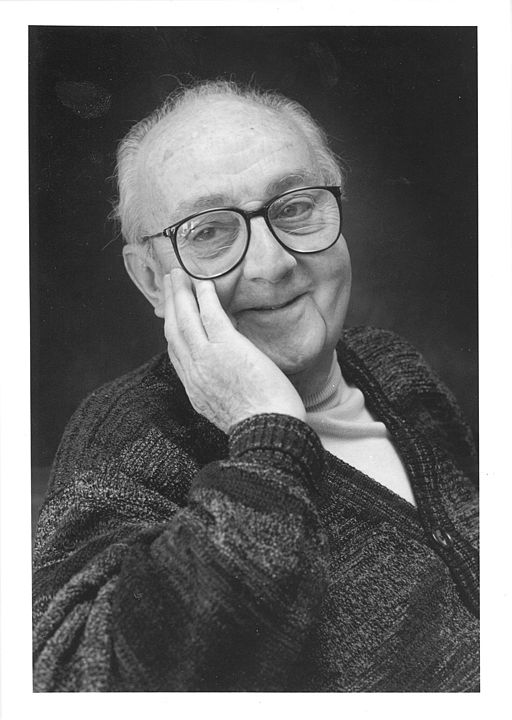
\includegraphics[width=0.9\columnwidth]{george_box.jpg}
        \end{column}
    \end{columns}
\end{frame}

\subsection{Fluxo de Trabalho Bayesiano (\textit{Workflow})\footnote{baseado em \textcite{gelmanBayesianWorkflow2020}}}
\begin{frame}{Fluxo de Trabalho Bayesiano (\textit{Workflow})\footnote{baseado em \textcite{gelmanBayesianWorkflow2020}}}
    \centering
    \begin{tikzpicture}[
        scale=0.8,
        transform shape, thick,
        every node/.style={text width=3.5cm, align=center},
        constructs/.style = {draw,
                            ellipse,
                            minimum width=4cm,
                            minimum height=2cm}
        ]
        \node[constructs] (Modelo) {Especificação do Modelo};
        \node[constructs] [right = of Modelo] (Priori) {Elicitação das \textit{Prioris}};
        \node[constructs] [right = of Priori] (Posterior) {Inferência da Posterior};
        \draw [<->, line width=1pt] (Modelo) to [out=45,in=135] node[above] {\textit{Prior Predictive Check}} (Priori);
        %\draw [->, line width=1pt] (Priori) to [out=225,in=315] {} (Modelo);
        \draw [<->, line width=1pt] (Priori) to [out=45,in=135] node[above] {\textit{Posterior Predictive Check}} (Posterior);
        %\draw [->, line width=1pt] (Posterior) to [out=225,in=315] {} (Priori);
    \end{tikzpicture}
\end{frame}

\subsection{Verificação Preditiva da \textit{Priori} (\textit{Prior Predictive Check})}
\begin{frame}{Verificação Preditiva da \textit{Priori} (\textit{Prior Predictive Check})}
    Em especial, antes de começar a alimentar o modelo com dados precisamos fazer uma
    checagem de todas as nossas \textit{prioris}.
    \vfill
    De maneira muito simples, consiste em simular parâmetros com base nas suas distribuições
    especificadas \textit{a priori} no modelo sem qualquer condicionamento aos dados e
    sem envolvimento nenhum da função de verossimilhança.
    \vfill
    Independentemente do nível de informação especificada na \textit{priori},
    é sempre importante realizar uma análise de sensibilidade prévia para entender completamente
    a influência que as \textit{prioris} têm na posterior.
\end{frame}

\begin{frame}{Verificação Preditiva da \textit{Priori} no \href{http://mc-stan.org/rstanarm/}{\texttt{rstanarm}} e \href{https://paul-buerkner.github.io/brms/}{\texttt{brms}}}
    \begin{vfilleditems}
        \item \texttt{rstanarm}: em qualquer função \text6t{stan\_*()} usar o argumento \texttt{prior\_PD = TRUE}
        \item \texttt{brms}: na função \textit{brm()} usar o argumento \texttt{sample\_prior = "only"}
    \end{vfilleditems}
\end{frame}

\subsubsection{Verificação Preditiva da \textit{Priori} no \texttt{rstanarm}}
\begin{frame}[fragile]{Verificação Preditiva da \textit{Priori} no \href{http://mc-stan.org/rstanarm/}{\texttt{rstanarm}}}
    \begin{lstlisting}
    stan_glm(y ~ ...,
        prior = normal(c(0, 0), c(5, 6)),
        prior_intercept = student_t(4, 0, 10),
        prior_aux = cauchy(0, 3),
        @prior_PD = TRUE@)
    \end{lstlisting}
\end{frame}
\subsubsection{Verificação Preditiva da \textit{Priori} no \texttt{brms}}
\begin{frame}[fragile]{Verificação Preditiva da \textit{Priori} no \href{https://paul-buerkner.github.io/brms/}{\texttt{brms}}}
    \begin{lstlisting}
    brm(y ~ x1 + x2,
        prior = c(
          prior(normal(0, 5), class = b, coef = x1),
          prior(normal(0, 6), class = b, coef = x2),
          prior(student_t(4, 0, 10), class = Intercept),
          prior(cauchy(0, 3), class = sigma)
        ),
        @sample_prior = "only"@)
    \end{lstlisting}
\end{frame}

\begin{frame}{Verificação Preditiva da \textit{Priori} no \href{https://paul-buerkner.github.io/brms/}{\texttt{brms}}}
    O interessante do \href{https://paul-buerkner.github.io/brms/}{\texttt{brms}} é
    que conseguimos naturalmente visualizar hipóteses sobre os valores do parâmetros de modelos
    estimados pela função \lstinline!brm()!
% library(brms)
% library(ggplot2)
% library(ggdark)
% library(bayesplot)
% library(tikzDevice)
% theme_set(dark_theme_light())
% bayesplot_theme_set(dark_theme_light())
% brms_custom_prior <- brm(mpg ~ wt + am, data = mtcars, chains = 1,
%  prior = c(
%    prior(normal(0, 5), class = b, coef = wt),
%    prior(normal(0, 6), class = b, coef = am),
%    prior(student_t(4, 0, 10), class = Intercept),
%    prior(cauchy(0, 3), class = sigma)
%  ),
%  sample_prior = "only")
% tikz(file = "slides/images/brms_prior_check.tex")
% plot(hypothesis(brms_custom_prior, "Intercept = 0"))
% dev.off()
    \begin{figure}
    \centering
        \resizebox{.35\linewidth}{!}{% Created by tikzDevice version 0.12.3.1 on 2021-05-29 18:08:38
% !TEX encoding = UTF-8 Unicode
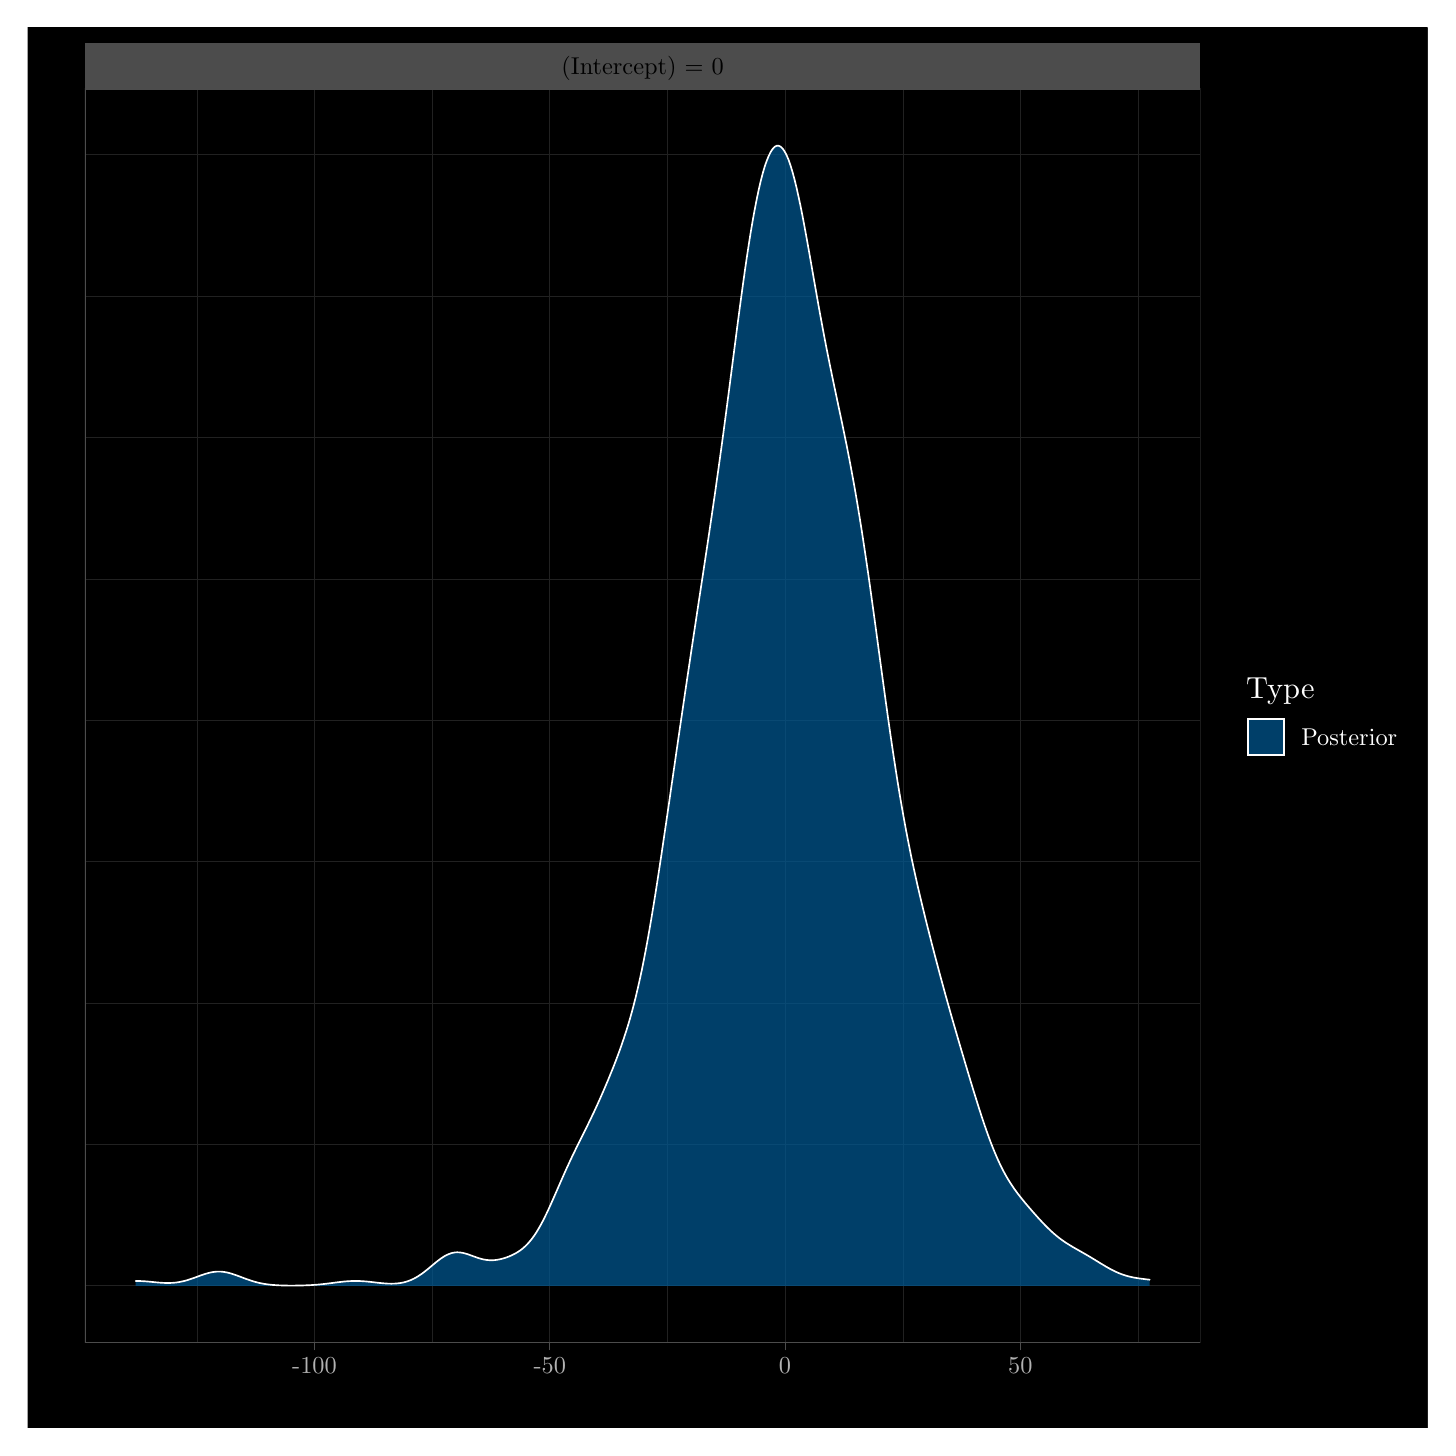
\begin{tikzpicture}[x=1pt,y=1pt]
\definecolor{fillColor}{RGB}{255,255,255}
\path[use as bounding box,fill=fillColor,fill opacity=0.00] (0,0) rectangle (505.89,505.89);
\begin{scope}
\path[clip] (  0.00,  0.00) rectangle (505.89,505.89);
\definecolor{drawColor}{RGB}{0,0,0}
\definecolor{fillColor}{RGB}{0,0,0}

\path[draw=drawColor,line width= 0.6pt,line join=round,line cap=round,fill=fillColor] (  0.00,  0.00) rectangle (505.89,505.89);
\end{scope}
\begin{scope}
\path[clip] ( 20.71, 30.69) rectangle (423.76,483.82);
\definecolor{fillColor}{RGB}{0,0,0}

\path[fill=fillColor] ( 20.71, 30.69) rectangle (423.76,483.82);
\definecolor{drawColor}{gray}{0.13}

\path[draw=drawColor,line width= 0.1pt,line join=round] ( 20.71,102.37) --
	(423.76,102.37);

\path[draw=drawColor,line width= 0.1pt,line join=round] ( 20.71,204.55) --
	(423.76,204.55);

\path[draw=drawColor,line width= 0.1pt,line join=round] ( 20.71,306.73) --
	(423.76,306.73);

\path[draw=drawColor,line width= 0.1pt,line join=round] ( 20.71,408.90) --
	(423.76,408.90);

\path[draw=drawColor,line width= 0.1pt,line join=round] ( 61.13, 30.69) --
	( 61.13,483.82);

\path[draw=drawColor,line width= 0.1pt,line join=round] (146.15, 30.69) --
	(146.15,483.82);

\path[draw=drawColor,line width= 0.1pt,line join=round] (231.17, 30.69) --
	(231.17,483.82);

\path[draw=drawColor,line width= 0.1pt,line join=round] (316.19, 30.69) --
	(316.19,483.82);

\path[draw=drawColor,line width= 0.1pt,line join=round] (401.21, 30.69) --
	(401.21,483.82);

\path[draw=drawColor,line width= 0.3pt,line join=round] ( 20.71, 51.28) --
	(423.76, 51.28);

\path[draw=drawColor,line width= 0.3pt,line join=round] ( 20.71,153.46) --
	(423.76,153.46);

\path[draw=drawColor,line width= 0.3pt,line join=round] ( 20.71,255.64) --
	(423.76,255.64);

\path[draw=drawColor,line width= 0.3pt,line join=round] ( 20.71,357.81) --
	(423.76,357.81);

\path[draw=drawColor,line width= 0.3pt,line join=round] ( 20.71,459.99) --
	(423.76,459.99);

\path[draw=drawColor,line width= 0.3pt,line join=round] (103.64, 30.69) --
	(103.64,483.82);

\path[draw=drawColor,line width= 0.3pt,line join=round] (188.66, 30.69) --
	(188.66,483.82);

\path[draw=drawColor,line width= 0.3pt,line join=round] (273.68, 30.69) --
	(273.68,483.82);

\path[draw=drawColor,line width= 0.3pt,line join=round] (358.70, 30.69) --
	(358.70,483.82);
\definecolor{fillColor}{RGB}{0,91,150}

\path[fill=fillColor,fill opacity=0.70] ( 39.03, 53.02) --
	( 39.75, 53.01) --
	( 40.47, 52.99) --
	( 41.19, 52.96) --
	( 41.90, 52.92) --
	( 42.62, 52.87) --
	( 43.34, 52.81) --
	( 44.05, 52.75) --
	( 44.77, 52.68) --
	( 45.49, 52.61) --
	( 46.20, 52.54) --
	( 46.92, 52.47) --
	( 47.64, 52.41) --
	( 48.36, 52.36) --
	( 49.07, 52.32) --
	( 49.79, 52.29) --
	( 50.51, 52.28) --
	( 51.22, 52.29) --
	( 51.94, 52.31) --
	( 52.66, 52.36) --
	( 53.38, 52.42) --
	( 54.09, 52.51) --
	( 54.81, 52.63) --
	( 55.53, 52.77) --
	( 56.24, 52.93) --
	( 56.96, 53.11) --
	( 57.68, 53.31) --
	( 58.39, 53.53) --
	( 59.11, 53.77) --
	( 59.83, 54.02) --
	( 60.55, 54.28) --
	( 61.26, 54.54) --
	( 61.98, 54.81) --
	( 62.70, 55.07) --
	( 63.41, 55.32) --
	( 64.13, 55.55) --
	( 64.85, 55.76) --
	( 65.56, 55.95) --
	( 66.28, 56.11) --
	( 67.00, 56.24) --
	( 67.72, 56.33) --
	( 68.43, 56.39) --
	( 69.15, 56.40) --
	( 69.87, 56.38) --
	( 70.58, 56.31) --
	( 71.30, 56.21) --
	( 72.02, 56.08) --
	( 72.73, 55.91) --
	( 73.45, 55.71) --
	( 74.17, 55.49) --
	( 74.89, 55.25) --
	( 75.60, 54.99) --
	( 76.32, 54.73) --
	( 77.04, 54.46) --
	( 77.75, 54.18) --
	( 78.47, 53.91) --
	( 79.19, 53.65) --
	( 79.91, 53.40) --
	( 80.62, 53.16) --
	( 81.34, 52.93) --
	( 82.06, 52.72) --
	( 82.77, 52.53) --
	( 83.49, 52.35) --
	( 84.21, 52.19) --
	( 84.92, 52.05) --
	( 85.64, 51.93) --
	( 86.36, 51.82) --
	( 87.08, 51.73) --
	( 87.79, 51.65) --
	( 88.51, 51.58) --
	( 89.23, 51.53) --
	( 89.94, 51.48) --
	( 90.66, 51.44) --
	( 91.38, 51.41) --
	( 92.09, 51.38) --
	( 92.81, 51.37) --
	( 93.53, 51.35) --
	( 94.25, 51.34) --
	( 94.96, 51.34) --
	( 95.68, 51.34) --
	( 96.40, 51.34) --
	( 97.11, 51.35) --
	( 97.83, 51.36) --
	( 98.55, 51.37) --
	( 99.27, 51.39) --
	( 99.98, 51.41) --
	(100.70, 51.44) --
	(101.42, 51.47) --
	(102.13, 51.50) --
	(102.85, 51.55) --
	(103.57, 51.60) --
	(104.28, 51.65) --
	(105.00, 51.71) --
	(105.72, 51.78) --
	(106.44, 51.85) --
	(107.15, 51.93) --
	(107.87, 52.01) --
	(108.59, 52.10) --
	(109.30, 52.19) --
	(110.02, 52.28) --
	(110.74, 52.37) --
	(111.45, 52.47) --
	(112.17, 52.56) --
	(112.89, 52.64) --
	(113.61, 52.72) --
	(114.32, 52.80) --
	(115.04, 52.86) --
	(115.76, 52.92) --
	(116.47, 52.96) --
	(117.19, 52.99) --
	(117.91, 53.01) --
	(118.62, 53.01) --
	(119.34, 53.00) --
	(120.06, 52.98) --
	(120.78, 52.94) --
	(121.49, 52.89) --
	(122.21, 52.84) --
	(122.93, 52.77) --
	(123.64, 52.70) --
	(124.36, 52.62) --
	(125.08, 52.54) --
	(125.80, 52.45) --
	(126.51, 52.37) --
	(127.23, 52.29) --
	(127.95, 52.22) --
	(128.66, 52.16) --
	(129.38, 52.11) --
	(130.10, 52.06) --
	(130.81, 52.04) --
	(131.53, 52.03) --
	(132.25, 52.05) --
	(132.97, 52.08) --
	(133.68, 52.14) --
	(134.40, 52.23) --
	(135.12, 52.34) --
	(135.83, 52.49) --
	(136.55, 52.68) --
	(137.27, 52.90) --
	(137.98, 53.15) --
	(138.70, 53.45) --
	(139.42, 53.79) --
	(140.14, 54.16) --
	(140.85, 54.58) --
	(141.57, 55.04) --
	(142.29, 55.53) --
	(143.00, 56.05) --
	(143.72, 56.60) --
	(144.44, 57.18) --
	(145.16, 57.77) --
	(145.87, 58.37) --
	(146.59, 58.98) --
	(147.31, 59.57) --
	(148.02, 60.15) --
	(148.74, 60.70) --
	(149.46, 61.22) --
	(150.17, 61.70) --
	(150.89, 62.12) --
	(151.61, 62.49) --
	(152.33, 62.79) --
	(153.04, 63.04) --
	(153.76, 63.22) --
	(154.48, 63.33) --
	(155.19, 63.37) --
	(155.91, 63.34) --
	(156.63, 63.26) --
	(157.34, 63.13) --
	(158.06, 62.95) --
	(158.78, 62.74) --
	(159.50, 62.50) --
	(160.21, 62.24) --
	(160.93, 61.98) --
	(161.65, 61.72) --
	(162.36, 61.47) --
	(163.08, 61.23) --
	(163.80, 61.02) --
	(164.51, 60.84) --
	(165.23, 60.70) --
	(165.95, 60.59) --
	(166.67, 60.53) --
	(167.38, 60.50) --
	(168.10, 60.51) --
	(168.82, 60.56) --
	(169.53, 60.65) --
	(170.25, 60.77) --
	(170.97, 60.92) --
	(171.69, 61.11) --
	(172.40, 61.32) --
	(173.12, 61.56) --
	(173.84, 61.83) --
	(174.55, 62.13) --
	(175.27, 62.46) --
	(175.99, 62.83) --
	(176.70, 63.23) --
	(177.42, 63.68) --
	(178.14, 64.18) --
	(178.86, 64.73) --
	(179.57, 65.36) --
	(180.29, 66.05) --
	(181.01, 66.81) --
	(181.72, 67.65) --
	(182.44, 68.57) --
	(183.16, 69.58) --
	(183.87, 70.67) --
	(184.59, 71.85) --
	(185.31, 73.11) --
	(186.03, 74.45) --
	(186.74, 75.85) --
	(187.46, 77.32) --
	(188.18, 78.84) --
	(188.89, 80.41) --
	(189.61, 82.02) --
	(190.33, 83.65) --
	(191.05, 85.29) --
	(191.76, 86.94) --
	(192.48, 88.58) --
	(193.20, 90.22) --
	(193.91, 91.83) --
	(194.63, 93.43) --
	(195.35, 94.99) --
	(196.06, 96.53) --
	(196.78, 98.05) --
	(197.50, 99.54) --
	(198.22,101.02) --
	(198.93,102.47) --
	(199.65,103.91) --
	(200.37,105.35) --
	(201.08,106.79) --
	(201.80,108.23) --
	(202.52,109.69) --
	(203.23,111.16) --
	(203.95,112.65) --
	(204.67,114.17) --
	(205.39,115.71) --
	(206.10,117.28) --
	(206.82,118.87) --
	(207.54,120.50) --
	(208.25,122.15) --
	(208.97,123.83) --
	(209.69,125.53) --
	(210.40,127.27) --
	(211.12,129.04) --
	(211.84,130.84) --
	(212.56,132.68) --
	(213.27,134.58) --
	(213.99,136.54) --
	(214.71,138.56) --
	(215.42,140.67) --
	(216.14,142.86) --
	(216.86,145.15) --
	(217.58,147.56) --
	(218.29,150.11) --
	(219.01,152.81) --
	(219.73,155.66) --
	(220.44,158.67) --
	(221.16,161.85) --
	(221.88,165.19) --
	(222.59,168.73) --
	(223.31,172.45) --
	(224.03,176.33) --
	(224.75,180.37) --
	(225.46,184.56) --
	(226.18,188.89) --
	(226.90,193.35) --
	(227.61,197.93) --
	(228.33,202.61) --
	(229.05,207.37) --
	(229.76,212.19) --
	(230.48,217.06) --
	(231.20,221.96) --
	(231.92,226.90) --
	(232.63,231.84) --
	(233.35,236.80) --
	(234.07,241.74) --
	(234.78,246.68) --
	(235.50,251.60) --
	(236.22,256.50) --
	(236.94,261.38) --
	(237.65,266.24) --
	(238.37,271.07) --
	(239.09,275.87) --
	(239.80,280.66) --
	(240.52,285.42) --
	(241.24,290.16) --
	(241.95,294.89) --
	(242.67,299.61) --
	(243.39,304.32) --
	(244.11,309.04) --
	(244.82,313.77) --
	(245.54,318.53) --
	(246.26,323.31) --
	(246.97,328.15) --
	(247.69,333.04) --
	(248.41,338.00) --
	(249.12,343.03) --
	(249.84,348.14) --
	(250.56,353.32) --
	(251.28,358.59) --
	(251.99,363.95) --
	(252.71,369.38) --
	(253.43,374.86) --
	(254.14,380.38) --
	(254.86,385.92) --
	(255.58,391.46) --
	(256.29,396.97) --
	(257.01,402.41) --
	(257.73,407.77) --
	(258.45,413.01) --
	(259.16,418.10) --
	(259.88,423.02) --
	(260.60,427.74) --
	(261.31,432.21) --
	(262.03,436.43) --
	(262.75,440.37) --
	(263.47,444.05) --
	(264.18,447.43) --
	(264.90,450.52) --
	(265.62,453.30) --
	(266.33,455.70) --
	(267.05,457.78) --
	(267.77,459.53) --
	(268.48,460.96) --
	(269.20,462.06) --
	(269.92,462.82) --
	(270.64,463.21) --
	(271.35,463.22) --
	(272.07,462.89) --
	(272.79,462.21) --
	(273.50,461.19) --
	(274.22,459.84) --
	(274.94,458.16) --
	(275.65,456.11) --
	(276.37,453.73) --
	(277.09,451.07) --
	(277.81,448.14) --
	(278.52,444.96) --
	(279.24,441.57) --
	(279.96,437.97) --
	(280.67,434.19) --
	(281.39,430.29) --
	(282.11,426.29) --
	(282.83,422.23) --
	(283.54,418.14) --
	(284.26,414.05) --
	(284.98,409.97) --
	(285.69,405.95) --
	(286.41,401.99) --
	(287.13,398.10) --
	(287.84,394.30) --
	(288.56,390.57) --
	(289.28,386.94) --
	(290.00,383.38) --
	(290.71,379.90) --
	(291.43,376.47) --
	(292.15,373.07) --
	(292.86,369.69) --
	(293.58,366.31) --
	(294.30,362.91) --
	(295.01,359.45) --
	(295.73,355.93) --
	(296.45,352.32) --
	(297.17,348.61) --
	(297.88,344.79) --
	(298.60,340.84) --
	(299.32,336.76) --
	(300.03,332.52) --
	(300.75,328.13) --
	(301.47,323.61) --
	(302.18,318.95) --
	(302.90,314.16) --
	(303.62,309.26) --
	(304.34,304.24) --
	(305.05,299.12) --
	(305.77,293.93) --
	(306.49,288.69) --
	(307.20,283.41) --
	(307.92,278.11) --
	(308.64,272.82) --
	(309.36,267.57) --
	(310.07,262.36) --
	(310.79,257.23) --
	(311.51,252.19) --
	(312.22,247.26) --
	(312.94,242.44) --
	(313.66,237.76) --
	(314.37,233.24) --
	(315.09,228.88) --
	(315.81,224.67) --
	(316.53,220.60) --
	(317.24,216.69) --
	(317.96,212.92) --
	(318.68,209.29) --
	(319.39,205.81) --
	(320.11,202.43) --
	(320.83,199.16) --
	(321.54,195.98) --
	(322.26,192.88) --
	(322.98,189.85) --
	(323.70,186.88) --
	(324.41,183.96) --
	(325.13,181.09) --
	(325.85,178.25) --
	(326.56,175.44) --
	(327.28,172.67) --
	(328.00,169.92) --
	(328.72,167.21) --
	(329.43,164.52) --
	(330.15,161.86) --
	(330.87,159.23) --
	(331.58,156.63) --
	(332.30,154.06) --
	(333.02,151.51) --
	(333.73,148.98) --
	(334.45,146.48) --
	(335.17,144.00) --
	(335.89,141.54) --
	(336.60,139.09) --
	(337.32,136.65) --
	(338.04,134.23) --
	(338.75,131.81) --
	(339.47,129.41) --
	(340.19,127.02) --
	(340.90,124.65) --
	(341.62,122.29) --
	(342.34,119.96) --
	(343.06,117.66) --
	(343.77,115.40) --
	(344.49,113.17) --
	(345.21,111.00) --
	(345.92,108.88) --
	(346.64,106.82) --
	(347.36,104.82) --
	(348.07,102.91) --
	(348.79,101.08) --
	(349.51, 99.33) --
	(350.23, 97.65) --
	(350.94, 96.06) --
	(351.66, 94.55) --
	(352.38, 93.12) --
	(353.09, 91.78) --
	(353.81, 90.51) --
	(354.53, 89.31) --
	(355.25, 88.17) --
	(355.96, 87.09) --
	(356.68, 86.06) --
	(357.40, 85.07) --
	(358.11, 84.13) --
	(358.83, 83.21) --
	(359.55, 82.32) --
	(360.26, 81.45) --
	(360.98, 80.59) --
	(361.70, 79.75) --
	(362.42, 78.92) --
	(363.13, 78.10) --
	(363.85, 77.28) --
	(364.57, 76.48) --
	(365.28, 75.68) --
	(366.00, 74.90) --
	(366.72, 74.13) --
	(367.43, 73.38) --
	(368.15, 72.65) --
	(368.87, 71.94) --
	(369.59, 71.25) --
	(370.30, 70.59) --
	(371.02, 69.96) --
	(371.74, 69.35) --
	(372.45, 68.77) --
	(373.17, 68.22) --
	(373.89, 67.70) --
	(374.61, 67.20) --
	(375.32, 66.73) --
	(376.04, 66.27) --
	(376.76, 65.83) --
	(377.47, 65.40) --
	(378.19, 64.98) --
	(378.91, 64.57) --
	(379.62, 64.17) --
	(380.34, 63.76) --
	(381.06, 63.35) --
	(381.78, 62.94) --
	(382.49, 62.53) --
	(383.21, 62.11) --
	(383.93, 61.68) --
	(384.64, 61.25) --
	(385.36, 60.81) --
	(386.08, 60.37) --
	(386.79, 59.93) --
	(387.51, 59.49) --
	(388.23, 59.06) --
	(388.95, 58.63) --
	(389.66, 58.20) --
	(390.38, 57.79) --
	(391.10, 57.39) --
	(391.81, 57.01) --
	(392.53, 56.65) --
	(393.25, 56.31) --
	(393.96, 55.99) --
	(394.68, 55.69) --
	(395.40, 55.42) --
	(396.12, 55.17) --
	(396.83, 54.95) --
	(397.55, 54.74) --
	(398.27, 54.56) --
	(398.98, 54.40) --
	(399.70, 54.25) --
	(400.42, 54.12) --
	(401.14, 54.01) --
	(401.85, 53.90) --
	(402.57, 53.81) --
	(403.29, 53.72) --
	(404.00, 53.63) --
	(404.72, 53.55) --
	(405.44, 53.46) --
	(405.44, 51.28) --
	(404.72, 51.28) --
	(404.00, 51.28) --
	(403.29, 51.28) --
	(402.57, 51.28) --
	(401.85, 51.28) --
	(401.14, 51.28) --
	(400.42, 51.28) --
	(399.70, 51.28) --
	(398.98, 51.28) --
	(398.27, 51.28) --
	(397.55, 51.28) --
	(396.83, 51.28) --
	(396.12, 51.28) --
	(395.40, 51.28) --
	(394.68, 51.28) --
	(393.96, 51.28) --
	(393.25, 51.28) --
	(392.53, 51.28) --
	(391.81, 51.28) --
	(391.10, 51.28) --
	(390.38, 51.28) --
	(389.66, 51.28) --
	(388.95, 51.28) --
	(388.23, 51.28) --
	(387.51, 51.28) --
	(386.79, 51.28) --
	(386.08, 51.28) --
	(385.36, 51.28) --
	(384.64, 51.28) --
	(383.93, 51.28) --
	(383.21, 51.28) --
	(382.49, 51.28) --
	(381.78, 51.28) --
	(381.06, 51.28) --
	(380.34, 51.28) --
	(379.62, 51.28) --
	(378.91, 51.28) --
	(378.19, 51.28) --
	(377.47, 51.28) --
	(376.76, 51.28) --
	(376.04, 51.28) --
	(375.32, 51.28) --
	(374.61, 51.28) --
	(373.89, 51.28) --
	(373.17, 51.28) --
	(372.45, 51.28) --
	(371.74, 51.28) --
	(371.02, 51.28) --
	(370.30, 51.28) --
	(369.59, 51.28) --
	(368.87, 51.28) --
	(368.15, 51.28) --
	(367.43, 51.28) --
	(366.72, 51.28) --
	(366.00, 51.28) --
	(365.28, 51.28) --
	(364.57, 51.28) --
	(363.85, 51.28) --
	(363.13, 51.28) --
	(362.42, 51.28) --
	(361.70, 51.28) --
	(360.98, 51.28) --
	(360.26, 51.28) --
	(359.55, 51.28) --
	(358.83, 51.28) --
	(358.11, 51.28) --
	(357.40, 51.28) --
	(356.68, 51.28) --
	(355.96, 51.28) --
	(355.25, 51.28) --
	(354.53, 51.28) --
	(353.81, 51.28) --
	(353.09, 51.28) --
	(352.38, 51.28) --
	(351.66, 51.28) --
	(350.94, 51.28) --
	(350.23, 51.28) --
	(349.51, 51.28) --
	(348.79, 51.28) --
	(348.07, 51.28) --
	(347.36, 51.28) --
	(346.64, 51.28) --
	(345.92, 51.28) --
	(345.21, 51.28) --
	(344.49, 51.28) --
	(343.77, 51.28) --
	(343.06, 51.28) --
	(342.34, 51.28) --
	(341.62, 51.28) --
	(340.90, 51.28) --
	(340.19, 51.28) --
	(339.47, 51.28) --
	(338.75, 51.28) --
	(338.04, 51.28) --
	(337.32, 51.28) --
	(336.60, 51.28) --
	(335.89, 51.28) --
	(335.17, 51.28) --
	(334.45, 51.28) --
	(333.73, 51.28) --
	(333.02, 51.28) --
	(332.30, 51.28) --
	(331.58, 51.28) --
	(330.87, 51.28) --
	(330.15, 51.28) --
	(329.43, 51.28) --
	(328.72, 51.28) --
	(328.00, 51.28) --
	(327.28, 51.28) --
	(326.56, 51.28) --
	(325.85, 51.28) --
	(325.13, 51.28) --
	(324.41, 51.28) --
	(323.70, 51.28) --
	(322.98, 51.28) --
	(322.26, 51.28) --
	(321.54, 51.28) --
	(320.83, 51.28) --
	(320.11, 51.28) --
	(319.39, 51.28) --
	(318.68, 51.28) --
	(317.96, 51.28) --
	(317.24, 51.28) --
	(316.53, 51.28) --
	(315.81, 51.28) --
	(315.09, 51.28) --
	(314.37, 51.28) --
	(313.66, 51.28) --
	(312.94, 51.28) --
	(312.22, 51.28) --
	(311.51, 51.28) --
	(310.79, 51.28) --
	(310.07, 51.28) --
	(309.36, 51.28) --
	(308.64, 51.28) --
	(307.92, 51.28) --
	(307.20, 51.28) --
	(306.49, 51.28) --
	(305.77, 51.28) --
	(305.05, 51.28) --
	(304.34, 51.28) --
	(303.62, 51.28) --
	(302.90, 51.28) --
	(302.18, 51.28) --
	(301.47, 51.28) --
	(300.75, 51.28) --
	(300.03, 51.28) --
	(299.32, 51.28) --
	(298.60, 51.28) --
	(297.88, 51.28) --
	(297.17, 51.28) --
	(296.45, 51.28) --
	(295.73, 51.28) --
	(295.01, 51.28) --
	(294.30, 51.28) --
	(293.58, 51.28) --
	(292.86, 51.28) --
	(292.15, 51.28) --
	(291.43, 51.28) --
	(290.71, 51.28) --
	(290.00, 51.28) --
	(289.28, 51.28) --
	(288.56, 51.28) --
	(287.84, 51.28) --
	(287.13, 51.28) --
	(286.41, 51.28) --
	(285.69, 51.28) --
	(284.98, 51.28) --
	(284.26, 51.28) --
	(283.54, 51.28) --
	(282.83, 51.28) --
	(282.11, 51.28) --
	(281.39, 51.28) --
	(280.67, 51.28) --
	(279.96, 51.28) --
	(279.24, 51.28) --
	(278.52, 51.28) --
	(277.81, 51.28) --
	(277.09, 51.28) --
	(276.37, 51.28) --
	(275.65, 51.28) --
	(274.94, 51.28) --
	(274.22, 51.28) --
	(273.50, 51.28) --
	(272.79, 51.28) --
	(272.07, 51.28) --
	(271.35, 51.28) --
	(270.64, 51.28) --
	(269.92, 51.28) --
	(269.20, 51.28) --
	(268.48, 51.28) --
	(267.77, 51.28) --
	(267.05, 51.28) --
	(266.33, 51.28) --
	(265.62, 51.28) --
	(264.90, 51.28) --
	(264.18, 51.28) --
	(263.47, 51.28) --
	(262.75, 51.28) --
	(262.03, 51.28) --
	(261.31, 51.28) --
	(260.60, 51.28) --
	(259.88, 51.28) --
	(259.16, 51.28) --
	(258.45, 51.28) --
	(257.73, 51.28) --
	(257.01, 51.28) --
	(256.29, 51.28) --
	(255.58, 51.28) --
	(254.86, 51.28) --
	(254.14, 51.28) --
	(253.43, 51.28) --
	(252.71, 51.28) --
	(251.99, 51.28) --
	(251.28, 51.28) --
	(250.56, 51.28) --
	(249.84, 51.28) --
	(249.12, 51.28) --
	(248.41, 51.28) --
	(247.69, 51.28) --
	(246.97, 51.28) --
	(246.26, 51.28) --
	(245.54, 51.28) --
	(244.82, 51.28) --
	(244.11, 51.28) --
	(243.39, 51.28) --
	(242.67, 51.28) --
	(241.95, 51.28) --
	(241.24, 51.28) --
	(240.52, 51.28) --
	(239.80, 51.28) --
	(239.09, 51.28) --
	(238.37, 51.28) --
	(237.65, 51.28) --
	(236.94, 51.28) --
	(236.22, 51.28) --
	(235.50, 51.28) --
	(234.78, 51.28) --
	(234.07, 51.28) --
	(233.35, 51.28) --
	(232.63, 51.28) --
	(231.92, 51.28) --
	(231.20, 51.28) --
	(230.48, 51.28) --
	(229.76, 51.28) --
	(229.05, 51.28) --
	(228.33, 51.28) --
	(227.61, 51.28) --
	(226.90, 51.28) --
	(226.18, 51.28) --
	(225.46, 51.28) --
	(224.75, 51.28) --
	(224.03, 51.28) --
	(223.31, 51.28) --
	(222.59, 51.28) --
	(221.88, 51.28) --
	(221.16, 51.28) --
	(220.44, 51.28) --
	(219.73, 51.28) --
	(219.01, 51.28) --
	(218.29, 51.28) --
	(217.58, 51.28) --
	(216.86, 51.28) --
	(216.14, 51.28) --
	(215.42, 51.28) --
	(214.71, 51.28) --
	(213.99, 51.28) --
	(213.27, 51.28) --
	(212.56, 51.28) --
	(211.84, 51.28) --
	(211.12, 51.28) --
	(210.40, 51.28) --
	(209.69, 51.28) --
	(208.97, 51.28) --
	(208.25, 51.28) --
	(207.54, 51.28) --
	(206.82, 51.28) --
	(206.10, 51.28) --
	(205.39, 51.28) --
	(204.67, 51.28) --
	(203.95, 51.28) --
	(203.23, 51.28) --
	(202.52, 51.28) --
	(201.80, 51.28) --
	(201.08, 51.28) --
	(200.37, 51.28) --
	(199.65, 51.28) --
	(198.93, 51.28) --
	(198.22, 51.28) --
	(197.50, 51.28) --
	(196.78, 51.28) --
	(196.06, 51.28) --
	(195.35, 51.28) --
	(194.63, 51.28) --
	(193.91, 51.28) --
	(193.20, 51.28) --
	(192.48, 51.28) --
	(191.76, 51.28) --
	(191.05, 51.28) --
	(190.33, 51.28) --
	(189.61, 51.28) --
	(188.89, 51.28) --
	(188.18, 51.28) --
	(187.46, 51.28) --
	(186.74, 51.28) --
	(186.03, 51.28) --
	(185.31, 51.28) --
	(184.59, 51.28) --
	(183.87, 51.28) --
	(183.16, 51.28) --
	(182.44, 51.28) --
	(181.72, 51.28) --
	(181.01, 51.28) --
	(180.29, 51.28) --
	(179.57, 51.28) --
	(178.86, 51.28) --
	(178.14, 51.28) --
	(177.42, 51.28) --
	(176.70, 51.28) --
	(175.99, 51.28) --
	(175.27, 51.28) --
	(174.55, 51.28) --
	(173.84, 51.28) --
	(173.12, 51.28) --
	(172.40, 51.28) --
	(171.69, 51.28) --
	(170.97, 51.28) --
	(170.25, 51.28) --
	(169.53, 51.28) --
	(168.82, 51.28) --
	(168.10, 51.28) --
	(167.38, 51.28) --
	(166.67, 51.28) --
	(165.95, 51.28) --
	(165.23, 51.28) --
	(164.51, 51.28) --
	(163.80, 51.28) --
	(163.08, 51.28) --
	(162.36, 51.28) --
	(161.65, 51.28) --
	(160.93, 51.28) --
	(160.21, 51.28) --
	(159.50, 51.28) --
	(158.78, 51.28) --
	(158.06, 51.28) --
	(157.34, 51.28) --
	(156.63, 51.28) --
	(155.91, 51.28) --
	(155.19, 51.28) --
	(154.48, 51.28) --
	(153.76, 51.28) --
	(153.04, 51.28) --
	(152.33, 51.28) --
	(151.61, 51.28) --
	(150.89, 51.28) --
	(150.17, 51.28) --
	(149.46, 51.28) --
	(148.74, 51.28) --
	(148.02, 51.28) --
	(147.31, 51.28) --
	(146.59, 51.28) --
	(145.87, 51.28) --
	(145.16, 51.28) --
	(144.44, 51.28) --
	(143.72, 51.28) --
	(143.00, 51.28) --
	(142.29, 51.28) --
	(141.57, 51.28) --
	(140.85, 51.28) --
	(140.14, 51.28) --
	(139.42, 51.28) --
	(138.70, 51.28) --
	(137.98, 51.28) --
	(137.27, 51.28) --
	(136.55, 51.28) --
	(135.83, 51.28) --
	(135.12, 51.28) --
	(134.40, 51.28) --
	(133.68, 51.28) --
	(132.97, 51.28) --
	(132.25, 51.28) --
	(131.53, 51.28) --
	(130.81, 51.28) --
	(130.10, 51.28) --
	(129.38, 51.28) --
	(128.66, 51.28) --
	(127.95, 51.28) --
	(127.23, 51.28) --
	(126.51, 51.28) --
	(125.80, 51.28) --
	(125.08, 51.28) --
	(124.36, 51.28) --
	(123.64, 51.28) --
	(122.93, 51.28) --
	(122.21, 51.28) --
	(121.49, 51.28) --
	(120.78, 51.28) --
	(120.06, 51.28) --
	(119.34, 51.28) --
	(118.62, 51.28) --
	(117.91, 51.28) --
	(117.19, 51.28) --
	(116.47, 51.28) --
	(115.76, 51.28) --
	(115.04, 51.28) --
	(114.32, 51.28) --
	(113.61, 51.28) --
	(112.89, 51.28) --
	(112.17, 51.28) --
	(111.45, 51.28) --
	(110.74, 51.28) --
	(110.02, 51.28) --
	(109.30, 51.28) --
	(108.59, 51.28) --
	(107.87, 51.28) --
	(107.15, 51.28) --
	(106.44, 51.28) --
	(105.72, 51.28) --
	(105.00, 51.28) --
	(104.28, 51.28) --
	(103.57, 51.28) --
	(102.85, 51.28) --
	(102.13, 51.28) --
	(101.42, 51.28) --
	(100.70, 51.28) --
	( 99.98, 51.28) --
	( 99.27, 51.28) --
	( 98.55, 51.28) --
	( 97.83, 51.28) --
	( 97.11, 51.28) --
	( 96.40, 51.28) --
	( 95.68, 51.28) --
	( 94.96, 51.28) --
	( 94.25, 51.28) --
	( 93.53, 51.28) --
	( 92.81, 51.28) --
	( 92.09, 51.28) --
	( 91.38, 51.28) --
	( 90.66, 51.28) --
	( 89.94, 51.28) --
	( 89.23, 51.28) --
	( 88.51, 51.28) --
	( 87.79, 51.28) --
	( 87.08, 51.28) --
	( 86.36, 51.28) --
	( 85.64, 51.28) --
	( 84.92, 51.28) --
	( 84.21, 51.28) --
	( 83.49, 51.28) --
	( 82.77, 51.28) --
	( 82.06, 51.28) --
	( 81.34, 51.28) --
	( 80.62, 51.28) --
	( 79.91, 51.28) --
	( 79.19, 51.28) --
	( 78.47, 51.28) --
	( 77.75, 51.28) --
	( 77.04, 51.28) --
	( 76.32, 51.28) --
	( 75.60, 51.28) --
	( 74.89, 51.28) --
	( 74.17, 51.28) --
	( 73.45, 51.28) --
	( 72.73, 51.28) --
	( 72.02, 51.28) --
	( 71.30, 51.28) --
	( 70.58, 51.28) --
	( 69.87, 51.28) --
	( 69.15, 51.28) --
	( 68.43, 51.28) --
	( 67.72, 51.28) --
	( 67.00, 51.28) --
	( 66.28, 51.28) --
	( 65.56, 51.28) --
	( 64.85, 51.28) --
	( 64.13, 51.28) --
	( 63.41, 51.28) --
	( 62.70, 51.28) --
	( 61.98, 51.28) --
	( 61.26, 51.28) --
	( 60.55, 51.28) --
	( 59.83, 51.28) --
	( 59.11, 51.28) --
	( 58.39, 51.28) --
	( 57.68, 51.28) --
	( 56.96, 51.28) --
	( 56.24, 51.28) --
	( 55.53, 51.28) --
	( 54.81, 51.28) --
	( 54.09, 51.28) --
	( 53.38, 51.28) --
	( 52.66, 51.28) --
	( 51.94, 51.28) --
	( 51.22, 51.28) --
	( 50.51, 51.28) --
	( 49.79, 51.28) --
	( 49.07, 51.28) --
	( 48.36, 51.28) --
	( 47.64, 51.28) --
	( 46.92, 51.28) --
	( 46.20, 51.28) --
	( 45.49, 51.28) --
	( 44.77, 51.28) --
	( 44.05, 51.28) --
	( 43.34, 51.28) --
	( 42.62, 51.28) --
	( 41.90, 51.28) --
	( 41.19, 51.28) --
	( 40.47, 51.28) --
	( 39.75, 51.28) --
	( 39.03, 51.28) --
	cycle;
\definecolor{drawColor}{RGB}{255,255,255}

\path[draw=drawColor,line width= 0.6pt,line join=round,line cap=round] ( 39.03, 53.02) --
	( 39.75, 53.01) --
	( 40.47, 52.99) --
	( 41.19, 52.96) --
	( 41.90, 52.92) --
	( 42.62, 52.87) --
	( 43.34, 52.81) --
	( 44.05, 52.75) --
	( 44.77, 52.68) --
	( 45.49, 52.61) --
	( 46.20, 52.54) --
	( 46.92, 52.47) --
	( 47.64, 52.41) --
	( 48.36, 52.36) --
	( 49.07, 52.32) --
	( 49.79, 52.29) --
	( 50.51, 52.28) --
	( 51.22, 52.29) --
	( 51.94, 52.31) --
	( 52.66, 52.36) --
	( 53.38, 52.42) --
	( 54.09, 52.51) --
	( 54.81, 52.63) --
	( 55.53, 52.77) --
	( 56.24, 52.93) --
	( 56.96, 53.11) --
	( 57.68, 53.31) --
	( 58.39, 53.53) --
	( 59.11, 53.77) --
	( 59.83, 54.02) --
	( 60.55, 54.28) --
	( 61.26, 54.54) --
	( 61.98, 54.81) --
	( 62.70, 55.07) --
	( 63.41, 55.32) --
	( 64.13, 55.55) --
	( 64.85, 55.76) --
	( 65.56, 55.95) --
	( 66.28, 56.11) --
	( 67.00, 56.24) --
	( 67.72, 56.33) --
	( 68.43, 56.39) --
	( 69.15, 56.40) --
	( 69.87, 56.38) --
	( 70.58, 56.31) --
	( 71.30, 56.21) --
	( 72.02, 56.08) --
	( 72.73, 55.91) --
	( 73.45, 55.71) --
	( 74.17, 55.49) --
	( 74.89, 55.25) --
	( 75.60, 54.99) --
	( 76.32, 54.73) --
	( 77.04, 54.46) --
	( 77.75, 54.18) --
	( 78.47, 53.91) --
	( 79.19, 53.65) --
	( 79.91, 53.40) --
	( 80.62, 53.16) --
	( 81.34, 52.93) --
	( 82.06, 52.72) --
	( 82.77, 52.53) --
	( 83.49, 52.35) --
	( 84.21, 52.19) --
	( 84.92, 52.05) --
	( 85.64, 51.93) --
	( 86.36, 51.82) --
	( 87.08, 51.73) --
	( 87.79, 51.65) --
	( 88.51, 51.58) --
	( 89.23, 51.53) --
	( 89.94, 51.48) --
	( 90.66, 51.44) --
	( 91.38, 51.41) --
	( 92.09, 51.38) --
	( 92.81, 51.37) --
	( 93.53, 51.35) --
	( 94.25, 51.34) --
	( 94.96, 51.34) --
	( 95.68, 51.34) --
	( 96.40, 51.34) --
	( 97.11, 51.35) --
	( 97.83, 51.36) --
	( 98.55, 51.37) --
	( 99.27, 51.39) --
	( 99.98, 51.41) --
	(100.70, 51.44) --
	(101.42, 51.47) --
	(102.13, 51.50) --
	(102.85, 51.55) --
	(103.57, 51.60) --
	(104.28, 51.65) --
	(105.00, 51.71) --
	(105.72, 51.78) --
	(106.44, 51.85) --
	(107.15, 51.93) --
	(107.87, 52.01) --
	(108.59, 52.10) --
	(109.30, 52.19) --
	(110.02, 52.28) --
	(110.74, 52.37) --
	(111.45, 52.47) --
	(112.17, 52.56) --
	(112.89, 52.64) --
	(113.61, 52.72) --
	(114.32, 52.80) --
	(115.04, 52.86) --
	(115.76, 52.92) --
	(116.47, 52.96) --
	(117.19, 52.99) --
	(117.91, 53.01) --
	(118.62, 53.01) --
	(119.34, 53.00) --
	(120.06, 52.98) --
	(120.78, 52.94) --
	(121.49, 52.89) --
	(122.21, 52.84) --
	(122.93, 52.77) --
	(123.64, 52.70) --
	(124.36, 52.62) --
	(125.08, 52.54) --
	(125.80, 52.45) --
	(126.51, 52.37) --
	(127.23, 52.29) --
	(127.95, 52.22) --
	(128.66, 52.16) --
	(129.38, 52.11) --
	(130.10, 52.06) --
	(130.81, 52.04) --
	(131.53, 52.03) --
	(132.25, 52.05) --
	(132.97, 52.08) --
	(133.68, 52.14) --
	(134.40, 52.23) --
	(135.12, 52.34) --
	(135.83, 52.49) --
	(136.55, 52.68) --
	(137.27, 52.90) --
	(137.98, 53.15) --
	(138.70, 53.45) --
	(139.42, 53.79) --
	(140.14, 54.16) --
	(140.85, 54.58) --
	(141.57, 55.04) --
	(142.29, 55.53) --
	(143.00, 56.05) --
	(143.72, 56.60) --
	(144.44, 57.18) --
	(145.16, 57.77) --
	(145.87, 58.37) --
	(146.59, 58.98) --
	(147.31, 59.57) --
	(148.02, 60.15) --
	(148.74, 60.70) --
	(149.46, 61.22) --
	(150.17, 61.70) --
	(150.89, 62.12) --
	(151.61, 62.49) --
	(152.33, 62.79) --
	(153.04, 63.04) --
	(153.76, 63.22) --
	(154.48, 63.33) --
	(155.19, 63.37) --
	(155.91, 63.34) --
	(156.63, 63.26) --
	(157.34, 63.13) --
	(158.06, 62.95) --
	(158.78, 62.74) --
	(159.50, 62.50) --
	(160.21, 62.24) --
	(160.93, 61.98) --
	(161.65, 61.72) --
	(162.36, 61.47) --
	(163.08, 61.23) --
	(163.80, 61.02) --
	(164.51, 60.84) --
	(165.23, 60.70) --
	(165.95, 60.59) --
	(166.67, 60.53) --
	(167.38, 60.50) --
	(168.10, 60.51) --
	(168.82, 60.56) --
	(169.53, 60.65) --
	(170.25, 60.77) --
	(170.97, 60.92) --
	(171.69, 61.11) --
	(172.40, 61.32) --
	(173.12, 61.56) --
	(173.84, 61.83) --
	(174.55, 62.13) --
	(175.27, 62.46) --
	(175.99, 62.83) --
	(176.70, 63.23) --
	(177.42, 63.68) --
	(178.14, 64.18) --
	(178.86, 64.73) --
	(179.57, 65.36) --
	(180.29, 66.05) --
	(181.01, 66.81) --
	(181.72, 67.65) --
	(182.44, 68.57) --
	(183.16, 69.58) --
	(183.87, 70.67) --
	(184.59, 71.85) --
	(185.31, 73.11) --
	(186.03, 74.45) --
	(186.74, 75.85) --
	(187.46, 77.32) --
	(188.18, 78.84) --
	(188.89, 80.41) --
	(189.61, 82.02) --
	(190.33, 83.65) --
	(191.05, 85.29) --
	(191.76, 86.94) --
	(192.48, 88.58) --
	(193.20, 90.22) --
	(193.91, 91.83) --
	(194.63, 93.43) --
	(195.35, 94.99) --
	(196.06, 96.53) --
	(196.78, 98.05) --
	(197.50, 99.54) --
	(198.22,101.02) --
	(198.93,102.47) --
	(199.65,103.91) --
	(200.37,105.35) --
	(201.08,106.79) --
	(201.80,108.23) --
	(202.52,109.69) --
	(203.23,111.16) --
	(203.95,112.65) --
	(204.67,114.17) --
	(205.39,115.71) --
	(206.10,117.28) --
	(206.82,118.87) --
	(207.54,120.50) --
	(208.25,122.15) --
	(208.97,123.83) --
	(209.69,125.53) --
	(210.40,127.27) --
	(211.12,129.04) --
	(211.84,130.84) --
	(212.56,132.68) --
	(213.27,134.58) --
	(213.99,136.54) --
	(214.71,138.56) --
	(215.42,140.67) --
	(216.14,142.86) --
	(216.86,145.15) --
	(217.58,147.56) --
	(218.29,150.11) --
	(219.01,152.81) --
	(219.73,155.66) --
	(220.44,158.67) --
	(221.16,161.85) --
	(221.88,165.19) --
	(222.59,168.73) --
	(223.31,172.45) --
	(224.03,176.33) --
	(224.75,180.37) --
	(225.46,184.56) --
	(226.18,188.89) --
	(226.90,193.35) --
	(227.61,197.93) --
	(228.33,202.61) --
	(229.05,207.37) --
	(229.76,212.19) --
	(230.48,217.06) --
	(231.20,221.96) --
	(231.92,226.90) --
	(232.63,231.84) --
	(233.35,236.80) --
	(234.07,241.74) --
	(234.78,246.68) --
	(235.50,251.60) --
	(236.22,256.50) --
	(236.94,261.38) --
	(237.65,266.24) --
	(238.37,271.07) --
	(239.09,275.87) --
	(239.80,280.66) --
	(240.52,285.42) --
	(241.24,290.16) --
	(241.95,294.89) --
	(242.67,299.61) --
	(243.39,304.32) --
	(244.11,309.04) --
	(244.82,313.77) --
	(245.54,318.53) --
	(246.26,323.31) --
	(246.97,328.15) --
	(247.69,333.04) --
	(248.41,338.00) --
	(249.12,343.03) --
	(249.84,348.14) --
	(250.56,353.32) --
	(251.28,358.59) --
	(251.99,363.95) --
	(252.71,369.38) --
	(253.43,374.86) --
	(254.14,380.38) --
	(254.86,385.92) --
	(255.58,391.46) --
	(256.29,396.97) --
	(257.01,402.41) --
	(257.73,407.77) --
	(258.45,413.01) --
	(259.16,418.10) --
	(259.88,423.02) --
	(260.60,427.74) --
	(261.31,432.21) --
	(262.03,436.43) --
	(262.75,440.37) --
	(263.47,444.05) --
	(264.18,447.43) --
	(264.90,450.52) --
	(265.62,453.30) --
	(266.33,455.70) --
	(267.05,457.78) --
	(267.77,459.53) --
	(268.48,460.96) --
	(269.20,462.06) --
	(269.92,462.82) --
	(270.64,463.21) --
	(271.35,463.22) --
	(272.07,462.89) --
	(272.79,462.21) --
	(273.50,461.19) --
	(274.22,459.84) --
	(274.94,458.16) --
	(275.65,456.11) --
	(276.37,453.73) --
	(277.09,451.07) --
	(277.81,448.14) --
	(278.52,444.96) --
	(279.24,441.57) --
	(279.96,437.97) --
	(280.67,434.19) --
	(281.39,430.29) --
	(282.11,426.29) --
	(282.83,422.23) --
	(283.54,418.14) --
	(284.26,414.05) --
	(284.98,409.97) --
	(285.69,405.95) --
	(286.41,401.99) --
	(287.13,398.10) --
	(287.84,394.30) --
	(288.56,390.57) --
	(289.28,386.94) --
	(290.00,383.38) --
	(290.71,379.90) --
	(291.43,376.47) --
	(292.15,373.07) --
	(292.86,369.69) --
	(293.58,366.31) --
	(294.30,362.91) --
	(295.01,359.45) --
	(295.73,355.93) --
	(296.45,352.32) --
	(297.17,348.61) --
	(297.88,344.79) --
	(298.60,340.84) --
	(299.32,336.76) --
	(300.03,332.52) --
	(300.75,328.13) --
	(301.47,323.61) --
	(302.18,318.95) --
	(302.90,314.16) --
	(303.62,309.26) --
	(304.34,304.24) --
	(305.05,299.12) --
	(305.77,293.93) --
	(306.49,288.69) --
	(307.20,283.41) --
	(307.92,278.11) --
	(308.64,272.82) --
	(309.36,267.57) --
	(310.07,262.36) --
	(310.79,257.23) --
	(311.51,252.19) --
	(312.22,247.26) --
	(312.94,242.44) --
	(313.66,237.76) --
	(314.37,233.24) --
	(315.09,228.88) --
	(315.81,224.67) --
	(316.53,220.60) --
	(317.24,216.69) --
	(317.96,212.92) --
	(318.68,209.29) --
	(319.39,205.81) --
	(320.11,202.43) --
	(320.83,199.16) --
	(321.54,195.98) --
	(322.26,192.88) --
	(322.98,189.85) --
	(323.70,186.88) --
	(324.41,183.96) --
	(325.13,181.09) --
	(325.85,178.25) --
	(326.56,175.44) --
	(327.28,172.67) --
	(328.00,169.92) --
	(328.72,167.21) --
	(329.43,164.52) --
	(330.15,161.86) --
	(330.87,159.23) --
	(331.58,156.63) --
	(332.30,154.06) --
	(333.02,151.51) --
	(333.73,148.98) --
	(334.45,146.48) --
	(335.17,144.00) --
	(335.89,141.54) --
	(336.60,139.09) --
	(337.32,136.65) --
	(338.04,134.23) --
	(338.75,131.81) --
	(339.47,129.41) --
	(340.19,127.02) --
	(340.90,124.65) --
	(341.62,122.29) --
	(342.34,119.96) --
	(343.06,117.66) --
	(343.77,115.40) --
	(344.49,113.17) --
	(345.21,111.00) --
	(345.92,108.88) --
	(346.64,106.82) --
	(347.36,104.82) --
	(348.07,102.91) --
	(348.79,101.08) --
	(349.51, 99.33) --
	(350.23, 97.65) --
	(350.94, 96.06) --
	(351.66, 94.55) --
	(352.38, 93.12) --
	(353.09, 91.78) --
	(353.81, 90.51) --
	(354.53, 89.31) --
	(355.25, 88.17) --
	(355.96, 87.09) --
	(356.68, 86.06) --
	(357.40, 85.07) --
	(358.11, 84.13) --
	(358.83, 83.21) --
	(359.55, 82.32) --
	(360.26, 81.45) --
	(360.98, 80.59) --
	(361.70, 79.75) --
	(362.42, 78.92) --
	(363.13, 78.10) --
	(363.85, 77.28) --
	(364.57, 76.48) --
	(365.28, 75.68) --
	(366.00, 74.90) --
	(366.72, 74.13) --
	(367.43, 73.38) --
	(368.15, 72.65) --
	(368.87, 71.94) --
	(369.59, 71.25) --
	(370.30, 70.59) --
	(371.02, 69.96) --
	(371.74, 69.35) --
	(372.45, 68.77) --
	(373.17, 68.22) --
	(373.89, 67.70) --
	(374.61, 67.20) --
	(375.32, 66.73) --
	(376.04, 66.27) --
	(376.76, 65.83) --
	(377.47, 65.40) --
	(378.19, 64.98) --
	(378.91, 64.57) --
	(379.62, 64.17) --
	(380.34, 63.76) --
	(381.06, 63.35) --
	(381.78, 62.94) --
	(382.49, 62.53) --
	(383.21, 62.11) --
	(383.93, 61.68) --
	(384.64, 61.25) --
	(385.36, 60.81) --
	(386.08, 60.37) --
	(386.79, 59.93) --
	(387.51, 59.49) --
	(388.23, 59.06) --
	(388.95, 58.63) --
	(389.66, 58.20) --
	(390.38, 57.79) --
	(391.10, 57.39) --
	(391.81, 57.01) --
	(392.53, 56.65) --
	(393.25, 56.31) --
	(393.96, 55.99) --
	(394.68, 55.69) --
	(395.40, 55.42) --
	(396.12, 55.17) --
	(396.83, 54.95) --
	(397.55, 54.74) --
	(398.27, 54.56) --
	(398.98, 54.40) --
	(399.70, 54.25) --
	(400.42, 54.12) --
	(401.14, 54.01) --
	(401.85, 53.90) --
	(402.57, 53.81) --
	(403.29, 53.72) --
	(404.00, 53.63) --
	(404.72, 53.55) --
	(405.44, 53.46);
\definecolor{drawColor}{RGB}{76,76,76}

\path[draw=drawColor,line width= 0.6pt,line join=round,line cap=round] ( 20.71, 30.69) rectangle (423.76,483.82);
\end{scope}
\begin{scope}
\path[clip] ( 20.71,483.82) rectangle (423.76,500.39);
\definecolor{fillColor}{RGB}{76,76,76}

\path[fill=fillColor] ( 20.71,483.82) rectangle (423.76,500.39);
\definecolor{drawColor}{RGB}{0,0,0}

\node[text=drawColor,anchor=base,inner sep=0pt, outer sep=0pt, scale=  0.88] at (222.24,489.07) {(Intercept) = 0};
\end{scope}
\begin{scope}
\path[clip] (  0.00,  0.00) rectangle (505.89,505.89);
\definecolor{drawColor}{RGB}{76,76,76}

\path[draw=drawColor,line width= 0.3pt,line join=round] (103.64, 27.94) --
	(103.64, 30.69);

\path[draw=drawColor,line width= 0.3pt,line join=round] (188.66, 27.94) --
	(188.66, 30.69);

\path[draw=drawColor,line width= 0.3pt,line join=round] (273.68, 27.94) --
	(273.68, 30.69);

\path[draw=drawColor,line width= 0.3pt,line join=round] (358.70, 27.94) --
	(358.70, 30.69);
\end{scope}
\begin{scope}
\path[clip] (  0.00,  0.00) rectangle (505.89,505.89);
\definecolor{drawColor}{RGB}{178,178,178}

\node[text=drawColor,anchor=base,inner sep=0pt, outer sep=0pt, scale=  0.88] at (103.64, 19.68) {-100};

\node[text=drawColor,anchor=base,inner sep=0pt, outer sep=0pt, scale=  0.88] at (188.66, 19.68) {-50};

\node[text=drawColor,anchor=base,inner sep=0pt, outer sep=0pt, scale=  0.88] at (273.68, 19.68) {0};

\node[text=drawColor,anchor=base,inner sep=0pt, outer sep=0pt, scale=  0.88] at (358.70, 19.68) {50};
\end{scope}
\begin{scope}
\path[clip] (  0.00,  0.00) rectangle (505.89,505.89);
\definecolor{fillColor}{RGB}{0,0,0}

\path[fill=fillColor] (434.76,236.92) rectangle (500.39,277.59);
\end{scope}
\begin{scope}
\path[clip] (  0.00,  0.00) rectangle (505.89,505.89);
\definecolor{drawColor}{RGB}{255,255,255}

\node[text=drawColor,anchor=base west,inner sep=0pt, outer sep=0pt, scale=  1.10] at (440.26,263.44) {Type};
\end{scope}
\begin{scope}
\path[clip] (  0.00,  0.00) rectangle (505.89,505.89);
\definecolor{fillColor}{RGB}{0,0,0}

\path[fill=fillColor] (440.26,242.42) rectangle (454.71,256.87);
\end{scope}
\begin{scope}
\path[clip] (  0.00,  0.00) rectangle (505.89,505.89);
\definecolor{drawColor}{RGB}{255,255,255}
\definecolor{fillColor}{RGB}{0,91,150}

\path[draw=drawColor,line width= 0.6pt,line cap=rect,fill=fillColor,fill opacity=0.70] (440.97,243.13) rectangle (454.00,256.16);
\end{scope}
\begin{scope}
\path[clip] (  0.00,  0.00) rectangle (505.89,505.89);
\definecolor{drawColor}{RGB}{255,255,255}

\node[text=drawColor,anchor=base west,inner sep=0pt, outer sep=0pt, scale=  0.88] at (460.21,246.61) {Posterior};
\end{scope}
\end{tikzpicture}
}
    \end{figure}
\end{frame}

\subsection{Verificação Preditiva da Posterior (\textit{Posterior Predictive Check})}
\begin{frame}{Verificação Preditiva da Posterior (\textit{Posterior Predictive Check})}
    Precisamos nos certificar que a nossa distribuição posterior de $\boldsymbol{y}$
    consegue capturar todas as nuanças da densidade real de $\boldsymbol{y}$.
    \vfill
    Isto é um procedimento chamado de Verificação Preditiva da Posterior
    (\textit{Posterior Predictive Check}) e é geralmente auferido com uma inspeção
    visual\footnote{também fazemos inspeções matemáticas probabilísticas,
    veja a seção de Comparação de Modelos} da densidade real de $\boldsymbol{y}$
    contrastada com amostragens da densidade
    posterior de $\boldsymbol{y}$ estimada pelo modelo Bayesiano.
    \vfill
    O propósito é comparar o histograma da variável dependente $\boldsymbol{y}$ contra o histograma variáveis dependentes simuladas
    pelo modelo $\boldsymbol{y}_{\text{rep}}$ após a estimação dos parâmetros. A ideia é
    que os histogramas reais e simulados se misturem e não haja divergências.
\end{frame}

\begin{frame}{Verificação Preditiva da Posterior no \href{http://mc-stan.org/rstanarm/}{\texttt{rstanarm}} e \href{https://paul-buerkner.github.io/brms/}{\texttt{brms}}}
    \begin{vfilleditems}
        \item \texttt{rstanarm}: função \lstinline!pp_check()! em qualquer modelo oriundo das funções \lstinline!stan_*()!
        \item \texttt{brms}: função \lstinline!pp_check()! em qualquer modelo oriundo da função \lstinline!brm()!
    \end{vfilleditems}
\end{frame}

\subsubsection{Verificação Preditiva da Posterior no \texttt{rstanarm}}
\begin{frame}[fragile]{Verificação Preditiva da Posterior no \href{http://mc-stan.org/rstanarm/}{\texttt{rstanarm}}}
    \begin{lstlisting}
    rstanarm_fit <- stan_glm(mpg ~ wt + am, data = mtcars)
    @pp_check(rstanarm_fit)@
    \end{lstlisting}
\end{frame}

\begin{frame}{Verificação Preditiva da Posterior no \href{http://mc-stan.org/rstanarm/}{\texttt{rstanarm}}}
% library(rstanarm)
% library(ggplot2)
% library(ggdark)
% library(bayesplot)
% library(tikzDevice)
% theme_set(dark_theme_light())
% bayesplot_theme_set(dark_theme_light())
% rstanarm_fit <- stan_glm(mpg ~ wt + am, data = mtcars)
% tikz(file = "slides/images/pp_check_rstanarm.tex")
% pp_check(rstanarm_fit, nreps = 10, seed = 123, type = "dens_overlay")
% dev.off()
    \begin{columns}
        \begin{column}{0.5\textwidth}
            \begin{figure}
                \centering
                \resizebox{0.8\columnwidth}{!}{% Created by tikzDevice version 0.12.3.1 on 2021-06-01 06:51:52
% !TEX encoding = UTF-8 Unicode
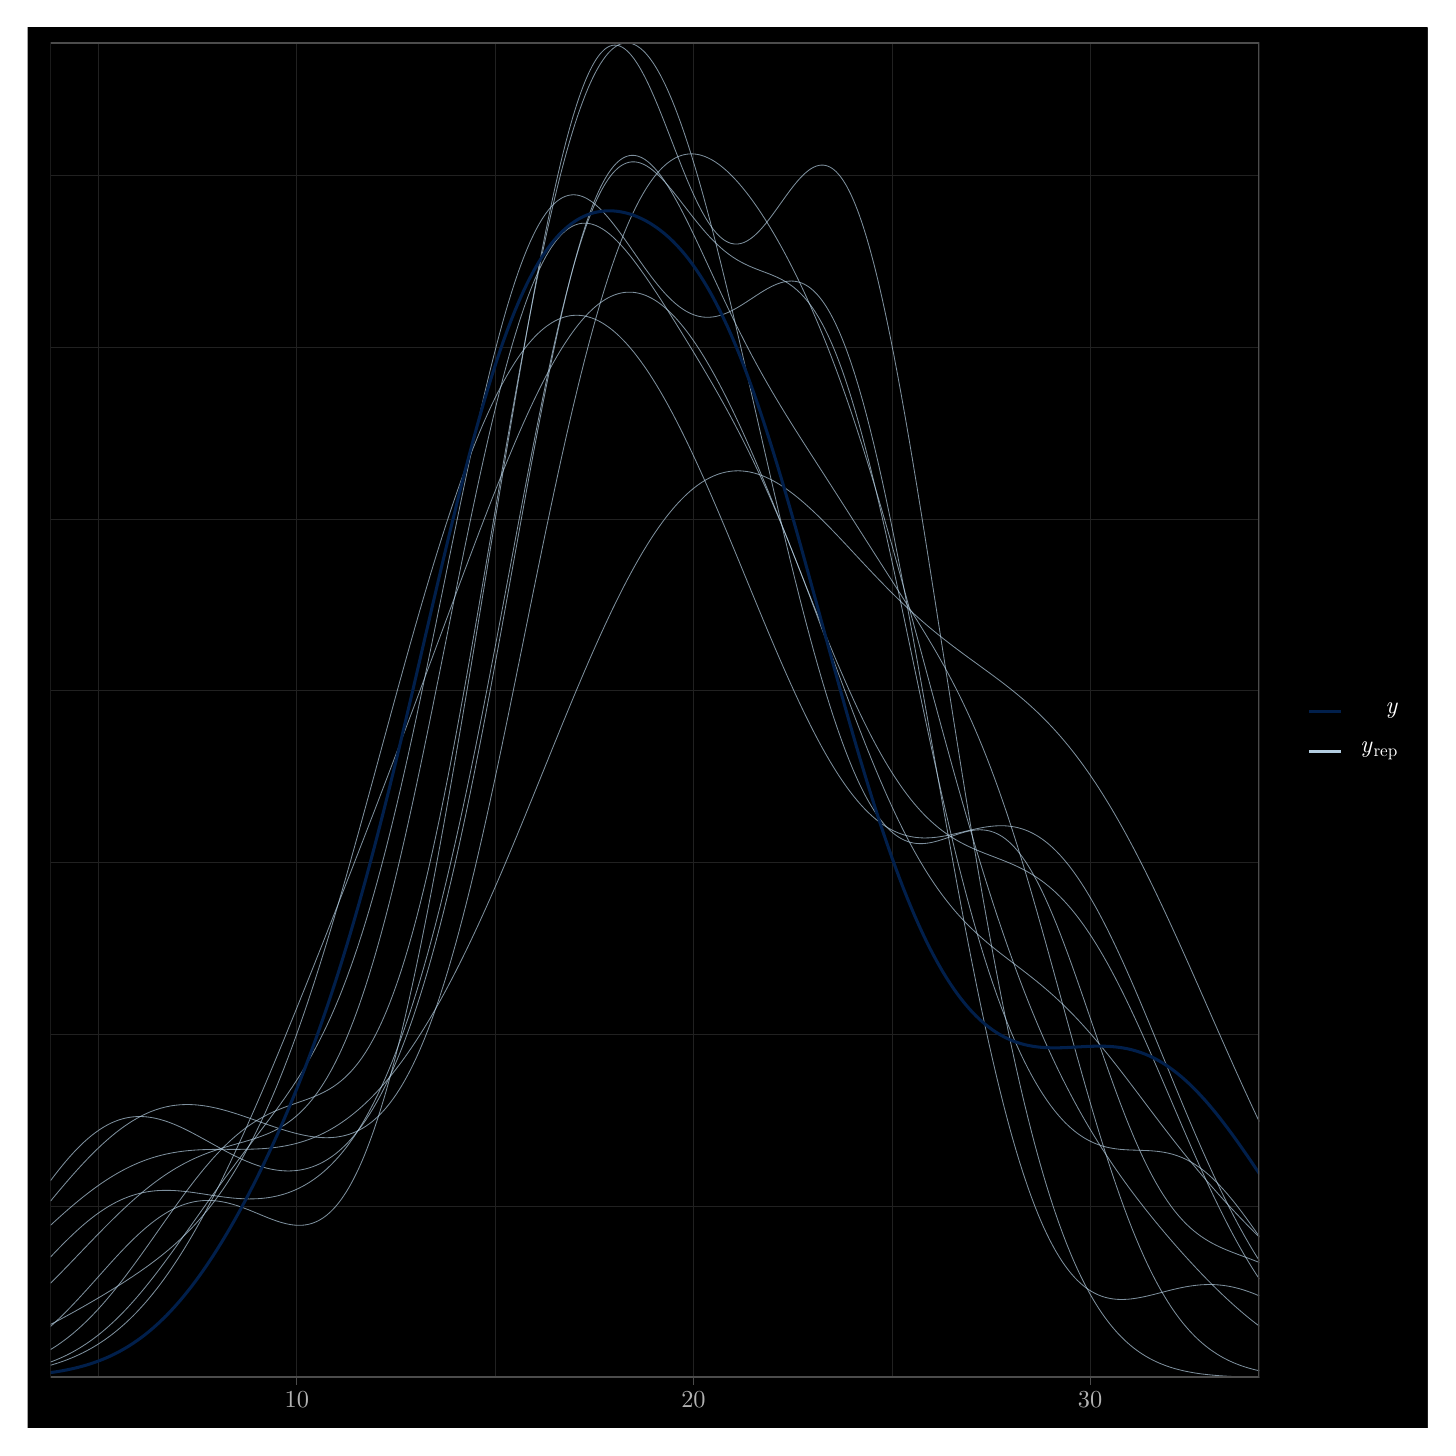
\begin{tikzpicture}[x=1pt,y=1pt]
\definecolor{fillColor}{RGB}{255,255,255}
\path[use as bounding box,fill=fillColor,fill opacity=0.00] (0,0) rectangle (505.89,505.89);
\begin{scope}
\path[clip] (  0.00,  0.00) rectangle (505.89,505.89);
\definecolor{drawColor}{RGB}{0,0,0}
\definecolor{fillColor}{RGB}{0,0,0}

\path[draw=drawColor,line width= 0.6pt,line join=round,line cap=round,fill=fillColor] (  0.00,  0.00) rectangle (505.89,505.89);
\end{scope}
\begin{scope}
\path[clip] (  8.25, 18.22) rectangle (445.03,500.39);
\definecolor{fillColor}{RGB}{0,0,0}

\path[fill=fillColor] (  8.25, 18.22) rectangle (445.03,500.39);
\definecolor{drawColor}{gray}{0.13}

\path[draw=drawColor,line width= 0.1pt,line join=round] (  8.25, 80.15) --
	(445.03, 80.15);

\path[draw=drawColor,line width= 0.1pt,line join=round] (  8.25,204.29) --
	(445.03,204.29);

\path[draw=drawColor,line width= 0.1pt,line join=round] (  8.25,328.43) --
	(445.03,328.43);

\path[draw=drawColor,line width= 0.1pt,line join=round] (  8.25,452.57) --
	(445.03,452.57);

\path[draw=drawColor,line width= 0.1pt,line join=round] ( 25.56, 18.22) --
	( 25.56,500.39);

\path[draw=drawColor,line width= 0.1pt,line join=round] (168.91, 18.22) --
	(168.91,500.39);

\path[draw=drawColor,line width= 0.1pt,line join=round] (312.26, 18.22) --
	(312.26,500.39);

\path[draw=drawColor,line width= 0.3pt,line join=round] (  8.25,142.22) --
	(445.03,142.22);

\path[draw=drawColor,line width= 0.3pt,line join=round] (  8.25,266.36) --
	(445.03,266.36);

\path[draw=drawColor,line width= 0.3pt,line join=round] (  8.25,390.50) --
	(445.03,390.50);

\path[draw=drawColor,line width= 0.3pt,line join=round] ( 97.24, 18.22) --
	( 97.24,500.39);

\path[draw=drawColor,line width= 0.3pt,line join=round] (240.58, 18.22) --
	(240.58,500.39);

\path[draw=drawColor,line width= 0.3pt,line join=round] (383.93, 18.22) --
	(383.93,500.39);
\definecolor{drawColor}{RGB}{179,205,224}

\path[draw=drawColor,draw opacity=0.70,line width= 0.3pt,line join=round] (  8.25, 81.87) --
	(  8.68, 82.38) --
	(  9.10, 82.90) --
	(  9.53, 83.42) --
	(  9.96, 83.93) --
	( 10.38, 84.44) --
	( 10.81, 84.96) --
	( 11.24, 85.47) --
	( 11.67, 85.97) --
	( 12.09, 86.48) --
	( 12.52, 86.98) --
	( 12.95, 87.49) --
	( 13.37, 87.99) --
	( 13.80, 88.48) --
	( 14.23, 88.98) --
	( 14.65, 89.47) --
	( 15.08, 89.97) --
	( 15.51, 90.45) --
	( 15.94, 90.94) --
	( 16.36, 91.42) --
	( 16.79, 91.91) --
	( 17.22, 92.38) --
	( 17.64, 92.86) --
	( 18.07, 93.33) --
	( 18.50, 93.80) --
	( 18.92, 94.27) --
	( 19.35, 94.73) --
	( 19.78, 95.19) --
	( 20.20, 95.65) --
	( 20.63, 96.10) --
	( 21.06, 96.55) --
	( 21.49, 97.00) --
	( 21.91, 97.44) --
	( 22.34, 97.88) --
	( 22.77, 98.32) --
	( 23.19, 98.75) --
	( 23.62, 99.18) --
	( 24.05, 99.60) --
	( 24.47,100.02) --
	( 24.90,100.44) --
	( 25.33,100.85) --
	( 25.76,101.26) --
	( 26.18,101.66) --
	( 26.61,102.06) --
	( 27.04,102.46) --
	( 27.46,102.85) --
	( 27.89,103.23) --
	( 28.32,103.61) --
	( 28.74,103.99) --
	( 29.17,104.36) --
	( 29.60,104.73) --
	( 30.02,105.09) --
	( 30.45,105.45) --
	( 30.88,105.80) --
	( 31.31,106.15) --
	( 31.73,106.49) --
	( 32.16,106.83) --
	( 32.59,107.16) --
	( 33.01,107.49) --
	( 33.44,107.81) --
	( 33.87,108.12) --
	( 34.29,108.44) --
	( 34.72,108.74) --
	( 35.15,109.04) --
	( 35.58,109.34) --
	( 36.00,109.62) --
	( 36.43,109.91) --
	( 36.86,110.19) --
	( 37.28,110.46) --
	( 37.71,110.73) --
	( 38.14,110.99) --
	( 38.56,111.24) --
	( 38.99,111.49) --
	( 39.42,111.74) --
	( 39.84,111.98) --
	( 40.27,112.21) --
	( 40.70,112.43) --
	( 41.13,112.66) --
	( 41.55,112.87) --
	( 41.98,113.08) --
	( 42.41,113.28) --
	( 42.83,113.48) --
	( 43.26,113.67) --
	( 43.69,113.86) --
	( 44.11,114.04) --
	( 44.54,114.21) --
	( 44.97,114.38) --
	( 45.40,114.54) --
	( 45.82,114.70) --
	( 46.25,114.85) --
	( 46.68,114.99) --
	( 47.10,115.13) --
	( 47.53,115.26) --
	( 47.96,115.39) --
	( 48.38,115.51) --
	( 48.81,115.62) --
	( 49.24,115.73) --
	( 49.66,115.84) --
	( 50.09,115.94) --
	( 50.52,116.03) --
	( 50.95,116.11) --
	( 51.37,116.20) --
	( 51.80,116.27) --
	( 52.23,116.34) --
	( 52.65,116.41) --
	( 53.08,116.46) --
	( 53.51,116.52) --
	( 53.93,116.56) --
	( 54.36,116.61) --
	( 54.79,116.65) --
	( 55.22,116.68) --
	( 55.64,116.70) --
	( 56.07,116.73) --
	( 56.50,116.74) --
	( 56.92,116.75) --
	( 57.35,116.76) --
	( 57.78,116.76) --
	( 58.20,116.76) --
	( 58.63,116.75) --
	( 59.06,116.74) --
	( 59.48,116.72) --
	( 59.91,116.70) --
	( 60.34,116.67) --
	( 60.77,116.64) --
	( 61.19,116.60) --
	( 61.62,116.56) --
	( 62.05,116.52) --
	( 62.47,116.47) --
	( 62.90,116.42) --
	( 63.33,116.36) --
	( 63.75,116.30) --
	( 64.18,116.24) --
	( 64.61,116.17) --
	( 65.04,116.10) --
	( 65.46,116.02) --
	( 65.89,115.94) --
	( 66.32,115.86) --
	( 66.74,115.77) --
	( 67.17,115.68) --
	( 67.60,115.59) --
	( 68.02,115.50) --
	( 68.45,115.40) --
	( 68.88,115.30) --
	( 69.30,115.19) --
	( 69.73,115.08) --
	( 70.16,114.97) --
	( 70.59,114.86) --
	( 71.01,114.74) --
	( 71.44,114.63) --
	( 71.87,114.51) --
	( 72.29,114.38) --
	( 72.72,114.26) --
	( 73.15,114.13) --
	( 73.57,114.00) --
	( 74.00,113.87) --
	( 74.43,113.74) --
	( 74.86,113.61) --
	( 75.28,113.47) --
	( 75.71,113.33) --
	( 76.14,113.19) --
	( 76.56,113.05) --
	( 76.99,112.91) --
	( 77.42,112.77) --
	( 77.84,112.62) --
	( 78.27,112.48) --
	( 78.70,112.33) --
	( 79.12,112.19) --
	( 79.55,112.04) --
	( 79.98,111.89) --
	( 80.41,111.74) --
	( 80.83,111.59) --
	( 81.26,111.44) --
	( 81.69,111.29) --
	( 82.11,111.14) --
	( 82.54,110.99) --
	( 82.97,110.84) --
	( 83.39,110.68) --
	( 83.82,110.53) --
	( 84.25,110.38) --
	( 84.68,110.23) --
	( 85.10,110.08) --
	( 85.53,109.93) --
	( 85.96,109.78) --
	( 86.38,109.63) --
	( 86.81,109.48) --
	( 87.24,109.33) --
	( 87.66,109.19) --
	( 88.09,109.04) --
	( 88.52,108.89) --
	( 88.94,108.75) --
	( 89.37,108.61) --
	( 89.80,108.46) --
	( 90.23,108.32) --
	( 90.65,108.18) --
	( 91.08,108.05) --
	( 91.51,107.91) --
	( 91.93,107.77) --
	( 92.36,107.64) --
	( 92.79,107.51) --
	( 93.21,107.38) --
	( 93.64,107.25) --
	( 94.07,107.13) --
	( 94.49,107.01) --
	( 94.92,106.88) --
	( 95.35,106.77) --
	( 95.78,106.65) --
	( 96.20,106.53) --
	( 96.63,106.42) --
	( 97.06,106.32) --
	( 97.48,106.21) --
	( 97.91,106.11) --
	( 98.34,106.01) --
	( 98.76,105.91) --
	( 99.19,105.82) --
	( 99.62,105.73) --
	(100.05,105.64) --
	(100.47,105.56) --
	(100.90,105.48) --
	(101.33,105.40) --
	(101.75,105.33) --
	(102.18,105.26) --
	(102.61,105.20) --
	(103.03,105.14) --
	(103.46,105.08) --
	(103.89,105.03) --
	(104.31,104.98) --
	(104.74,104.94) --
	(105.17,104.90) --
	(105.60,104.87) --
	(106.02,104.84) --
	(106.45,104.82) --
	(106.88,104.80) --
	(107.30,104.79) --
	(107.73,104.79) --
	(108.16,104.79) --
	(108.58,104.79) --
	(109.01,104.80) --
	(109.44,104.82) --
	(109.87,104.84) --
	(110.29,104.87) --
	(110.72,104.91) --
	(111.15,104.95) --
	(111.57,105.00) --
	(112.00,105.06) --
	(112.43,105.13) --
	(112.85,105.20) --
	(113.28,105.28) --
	(113.71,105.36) --
	(114.13,105.46) --
	(114.56,105.56) --
	(114.99,105.67) --
	(115.42,105.79) --
	(115.84,105.92) --
	(116.27,106.05) --
	(116.70,106.20) --
	(117.12,106.35) --
	(117.55,106.51) --
	(117.98,106.69) --
	(118.40,106.87) --
	(118.83,107.06) --
	(119.26,107.26) --
	(119.69,107.47) --
	(120.11,107.70) --
	(120.54,107.93) --
	(120.97,108.17) --
	(121.39,108.43) --
	(121.82,108.69) --
	(122.25,108.97) --
	(122.67,109.26) --
	(123.10,109.55) --
	(123.53,109.87) --
	(123.95,110.19) --
	(124.38,110.52) --
	(124.81,110.87) --
	(125.24,111.23) --
	(125.66,111.61) --
	(126.09,111.99) --
	(126.52,112.39) --
	(126.94,112.80) --
	(127.37,113.23) --
	(127.80,113.67) --
	(128.22,114.12) --
	(128.65,114.59) --
	(129.08,115.07) --
	(129.51,115.57) --
	(129.93,116.08) --
	(130.36,116.61) --
	(130.79,117.15) --
	(131.21,117.70) --
	(131.64,118.28) --
	(132.07,118.86) --
	(132.49,119.46) --
	(132.92,120.08) --
	(133.35,120.71) --
	(133.77,121.37) --
	(134.20,122.03) --
	(134.63,122.71) --
	(135.06,123.41) --
	(135.48,124.13) --
	(135.91,124.86) --
	(136.34,125.61) --
	(136.76,126.38) --
	(137.19,127.17) --
	(137.62,127.97) --
	(138.04,128.78) --
	(138.47,129.62) --
	(138.90,130.47) --
	(139.33,131.35) --
	(139.75,132.24) --
	(140.18,133.14) --
	(140.61,134.08) --
	(141.03,135.02) --
	(141.46,135.98) --
	(141.89,136.96) --
	(142.31,137.96) --
	(142.74,138.98) --
	(143.17,140.02) --
	(143.59,141.07) --
	(144.02,142.15) --
	(144.45,143.24) --
	(144.88,144.35) --
	(145.30,145.48) --
	(145.73,146.63) --
	(146.16,147.80) --
	(146.58,148.98) --
	(147.01,150.19) --
	(147.44,151.41) --
	(147.86,152.65) --
	(148.29,153.92) --
	(148.72,155.20) --
	(149.15,156.49) --
	(149.57,157.81) --
	(150.00,159.15) --
	(150.43,160.50) --
	(150.85,161.87) --
	(151.28,163.26) --
	(151.71,164.67) --
	(152.13,166.10) --
	(152.56,167.54) --
	(152.99,169.01) --
	(153.41,170.49) --
	(153.84,171.99) --
	(154.27,173.51) --
	(154.70,175.03) --
	(155.12,176.59) --
	(155.55,178.16) --
	(155.98,179.74) --
	(156.40,181.35) --
	(156.83,182.96) --
	(157.26,184.60) --
	(157.68,186.25) --
	(158.11,187.92) --
	(158.54,189.61) --
	(158.97,191.30) --
	(159.39,193.02) --
	(159.82,194.75) --
	(160.25,196.49) --
	(160.67,198.26) --
	(161.10,200.03) --
	(161.53,201.82) --
	(161.95,203.63) --
	(162.38,205.44) --
	(162.81,207.27) --
	(163.23,209.12) --
	(163.66,210.97) --
	(164.09,212.85) --
	(164.52,214.73) --
	(164.94,216.62) --
	(165.37,218.53) --
	(165.80,220.45) --
	(166.22,222.38) --
	(166.65,224.32) --
	(167.08,226.27) --
	(167.50,228.24) --
	(167.93,230.21) --
	(168.36,232.19) --
	(168.79,234.18) --
	(169.21,236.18) --
	(169.64,238.19) --
	(170.07,240.21) --
	(170.49,242.24) --
	(170.92,244.27) --
	(171.35,246.31) --
	(171.77,248.36) --
	(172.20,250.41) --
	(172.63,252.47) --
	(173.05,254.54) --
	(173.48,256.61) --
	(173.91,258.69) --
	(174.34,260.77) --
	(174.76,262.86) --
	(175.19,264.95) --
	(175.62,267.05) --
	(176.04,269.14) --
	(176.47,271.24) --
	(176.90,273.35) --
	(177.32,275.45) --
	(177.75,277.56) --
	(178.18,279.67) --
	(178.61,281.78) --
	(179.03,283.89) --
	(179.46,286.00) --
	(179.89,288.11) --
	(180.31,290.22) --
	(180.74,292.33) --
	(181.17,294.44) --
	(181.59,296.55) --
	(182.02,298.65) --
	(182.45,300.75) --
	(182.87,302.85) --
	(183.30,304.95) --
	(183.73,307.04) --
	(184.16,309.13) --
	(184.58,311.22) --
	(185.01,313.30) --
	(185.44,315.37) --
	(185.86,317.44) --
	(186.29,319.51) --
	(186.72,321.57) --
	(187.14,323.62) --
	(187.57,325.67) --
	(188.00,327.70) --
	(188.43,329.74) --
	(188.85,331.76) --
	(189.28,333.78) --
	(189.71,335.78) --
	(190.13,337.78) --
	(190.56,339.77) --
	(190.99,341.75) --
	(191.41,343.72) --
	(191.84,345.69) --
	(192.27,347.64) --
	(192.69,349.58) --
	(193.12,351.51) --
	(193.55,353.42) --
	(193.98,355.33) --
	(194.40,357.23) --
	(194.83,359.11) --
	(195.26,360.98) --
	(195.68,362.84) --
	(196.11,364.69) --
	(196.54,366.52) --
	(196.96,368.34) --
	(197.39,370.14) --
	(197.82,371.93) --
	(198.25,373.71) --
	(198.67,375.48) --
	(199.10,377.22) --
	(199.53,378.96) --
	(199.95,380.68) --
	(200.38,382.38) --
	(200.81,384.07) --
	(201.23,385.74) --
	(201.66,387.40) --
	(202.09,389.04) --
	(202.51,390.66) --
	(202.94,392.27) --
	(203.37,393.86) --
	(203.80,395.43) --
	(204.22,397.00) --
	(204.65,398.53) --
	(205.08,400.06) --
	(205.50,401.56) --
	(205.93,403.05) --
	(206.36,404.52) --
	(206.78,405.97) --
	(207.21,407.41) --
	(207.64,408.82) --
	(208.07,410.22) --
	(208.49,411.60) --
	(208.92,412.96) --
	(209.35,414.30) --
	(209.77,415.63) --
	(210.20,416.93) --
	(210.63,418.21) --
	(211.05,419.48) --
	(211.48,420.73) --
	(211.91,421.96) --
	(212.33,423.16) --
	(212.76,424.35) --
	(213.19,425.53) --
	(213.62,426.67) --
	(214.04,427.80) --
	(214.47,428.91) --
	(214.90,430.00) --
	(215.32,431.08) --
	(215.75,432.13) --
	(216.18,433.16) --
	(216.60,434.17) --
	(217.03,435.16) --
	(217.46,436.14) --
	(217.89,437.09) --
	(218.31,438.02) --
	(218.74,438.94) --
	(219.17,439.82) --
	(219.59,440.70) --
	(220.02,441.55) --
	(220.45,442.38) --
	(220.87,443.20) --
	(221.30,443.99) --
	(221.73,444.76) --
	(222.15,445.52) --
	(222.58,446.25) --
	(223.01,446.97) --
	(223.44,447.66) --
	(223.86,448.33) --
	(224.29,448.99) --
	(224.72,449.63) --
	(225.14,450.24) --
	(225.57,450.84) --
	(226.00,451.42) --
	(226.42,451.98) --
	(226.85,452.52) --
	(227.28,453.04) --
	(227.71,453.54) --
	(228.13,454.02) --
	(228.56,454.48) --
	(228.99,454.93) --
	(229.41,455.35) --
	(229.84,455.76) --
	(230.27,456.15) --
	(230.69,456.52) --
	(231.12,456.88) --
	(231.55,457.21) --
	(231.97,457.52) --
	(232.40,457.82) --
	(232.83,458.10) --
	(233.26,458.37) --
	(233.68,458.61) --
	(234.11,458.84) --
	(234.54,459.05) --
	(234.96,459.24) --
	(235.39,459.42) --
	(235.82,459.58) --
	(236.24,459.72) --
	(236.67,459.85) --
	(237.10,459.95) --
	(237.53,460.05) --
	(237.95,460.13) --
	(238.38,460.19) --
	(238.81,460.23) --
	(239.23,460.26) --
	(239.66,460.27) --
	(240.09,460.28) --
	(240.51,460.26) --
	(240.94,460.23) --
	(241.37,460.18) --
	(241.79,460.12) --
	(242.22,460.04) --
	(242.65,459.95) --
	(243.08,459.85) --
	(243.50,459.73) --
	(243.93,459.59) --
	(244.36,459.45) --
	(244.78,459.29) --
	(245.21,459.11) --
	(245.64,458.93) --
	(246.06,458.73) --
	(246.49,458.51) --
	(246.92,458.29) --
	(247.35,458.05) --
	(247.77,457.80) --
	(248.20,457.54) --
	(248.63,457.26) --
	(249.05,456.97) --
	(249.48,456.67) --
	(249.91,456.36) --
	(250.33,456.04) --
	(250.76,455.70) --
	(251.19,455.36) --
	(251.61,455.00) --
	(252.04,454.63) --
	(252.47,454.26) --
	(252.90,453.87) --
	(253.32,453.47) --
	(253.75,453.06) --
	(254.18,452.64) --
	(254.60,452.21) --
	(255.03,451.77) --
	(255.46,451.31) --
	(255.88,450.86) --
	(256.31,450.39) --
	(256.74,449.91) --
	(257.17,449.42) --
	(257.59,448.92) --
	(258.02,448.41) --
	(258.45,447.90) --
	(258.87,447.37) --
	(259.30,446.84) --
	(259.73,446.30) --
	(260.15,445.75) --
	(260.58,445.19) --
	(261.01,444.62) --
	(261.43,444.04) --
	(261.86,443.46) --
	(262.29,442.86) --
	(262.72,442.26) --
	(263.14,441.65) --
	(263.57,441.04) --
	(264.00,440.41) --
	(264.42,439.78) --
	(264.85,439.14) --
	(265.28,438.49) --
	(265.70,437.83) --
	(266.13,437.17) --
	(266.56,436.50) --
	(266.98,435.82) --
	(267.41,435.13) --
	(267.84,434.44) --
	(268.27,433.74) --
	(268.69,433.03) --
	(269.12,432.31) --
	(269.55,431.59) --
	(269.97,430.86) --
	(270.40,430.12) --
	(270.83,429.37) --
	(271.25,428.62) --
	(271.68,427.86) --
	(272.11,427.09) --
	(272.54,426.32) --
	(272.96,425.54) --
	(273.39,424.75) --
	(273.82,423.95) --
	(274.24,423.14) --
	(274.67,422.33) --
	(275.10,421.51) --
	(275.52,420.69) --
	(275.95,419.85) --
	(276.38,419.01) --
	(276.80,418.16) --
	(277.23,417.31) --
	(277.66,416.44) --
	(278.09,415.57) --
	(278.51,414.69) --
	(278.94,413.80) --
	(279.37,412.91) --
	(279.79,412.00) --
	(280.22,411.09) --
	(280.65,410.18) --
	(281.07,409.25) --
	(281.50,408.31) --
	(281.93,407.37) --
	(282.36,406.42) --
	(282.78,405.46) --
	(283.21,404.50) --
	(283.64,403.52) --
	(284.06,402.54) --
	(284.49,401.55) --
	(284.92,400.55) --
	(285.34,399.54) --
	(285.77,398.52) --
	(286.20,397.50) --
	(286.62,396.47) --
	(287.05,395.43) --
	(287.48,394.38) --
	(287.91,393.32) --
	(288.33,392.25) --
	(288.76,391.18) --
	(289.19,390.09) --
	(289.61,389.00) --
	(290.04,387.90) --
	(290.47,386.79) --
	(290.89,385.67) --
	(291.32,384.54) --
	(291.75,383.41) --
	(292.18,382.26) --
	(292.60,381.10) --
	(293.03,379.94) --
	(293.46,378.77) --
	(293.88,377.59) --
	(294.31,376.40) --
	(294.74,375.20) --
	(295.16,374.00) --
	(295.59,372.78) --
	(296.02,371.55) --
	(296.44,370.32) --
	(296.87,369.08) --
	(297.30,367.83) --
	(297.73,366.57) --
	(298.15,365.30) --
	(298.58,364.03) --
	(299.01,362.74) --
	(299.43,361.45) --
	(299.86,360.14) --
	(300.29,358.83) --
	(300.71,357.51) --
	(301.14,356.19) --
	(301.57,354.85) --
	(302.00,353.51) --
	(302.42,352.15) --
	(302.85,350.80) --
	(303.28,349.43) --
	(303.70,348.05) --
	(304.13,346.67) --
	(304.56,345.28) --
	(304.98,343.88) --
	(305.41,342.47) --
	(305.84,341.06) --
	(306.26,339.64) --
	(306.69,338.21) --
	(307.12,336.77) --
	(307.55,335.33) --
	(307.97,333.88) --
	(308.40,332.43) --
	(308.83,330.97) --
	(309.25,329.50) --
	(309.68,328.02) --
	(310.11,326.54) --
	(310.53,325.05) --
	(310.96,323.56) --
	(311.39,322.06) --
	(311.82,320.56) --
	(312.24,319.05) --
	(312.67,317.54) --
	(313.10,316.02) --
	(313.52,314.49) --
	(313.95,312.96) --
	(314.38,311.43) --
	(314.80,309.89) --
	(315.23,308.35) --
	(315.66,306.81) --
	(316.08,305.26) --
	(316.51,303.70) --
	(316.94,302.15) --
	(317.37,300.59) --
	(317.79,299.02) --
	(318.22,297.46) --
	(318.65,295.89) --
	(319.07,294.32) --
	(319.50,292.74) --
	(319.93,291.17) --
	(320.35,289.59) --
	(320.78,288.01) --
	(321.21,286.43) --
	(321.64,284.85) --
	(322.06,283.27) --
	(322.49,281.68) --
	(322.92,280.10) --
	(323.34,278.52) --
	(323.77,276.93) --
	(324.20,275.34) --
	(324.62,273.76) --
	(325.05,272.17) --
	(325.48,270.59) --
	(325.90,269.01) --
	(326.33,267.42) --
	(326.76,265.84) --
	(327.19,264.26) --
	(327.61,262.68) --
	(328.04,261.10) --
	(328.47,259.53) --
	(328.89,257.95) --
	(329.32,256.38) --
	(329.75,254.81) --
	(330.17,253.25) --
	(330.60,251.68) --
	(331.03,250.12) --
	(331.46,248.56) --
	(331.88,247.01) --
	(332.31,245.46) --
	(332.74,243.91) --
	(333.16,242.36) --
	(333.59,240.82) --
	(334.02,239.29) --
	(334.44,237.76) --
	(334.87,236.23) --
	(335.30,234.71) --
	(335.72,233.19) --
	(336.15,231.68) --
	(336.58,230.17) --
	(337.01,228.66) --
	(337.43,227.17) --
	(337.86,225.67) --
	(338.29,224.19) --
	(338.71,222.71) --
	(339.14,221.23) --
	(339.57,219.76) --
	(339.99,218.30) --
	(340.42,216.84) --
	(340.85,215.39) --
	(341.28,213.94) --
	(341.70,212.51) --
	(342.13,211.07) --
	(342.56,209.65) --
	(342.98,208.23) --
	(343.41,206.82) --
	(343.84,205.42) --
	(344.26,204.02) --
	(344.69,202.63) --
	(345.12,201.25) --
	(345.54,199.87) --
	(345.97,198.50) --
	(346.40,197.14) --
	(346.83,195.79) --
	(347.25,194.44) --
	(347.68,193.10) --
	(348.11,191.77) --
	(348.53,190.45) --
	(348.96,189.13) --
	(349.39,187.83) --
	(349.81,186.53) --
	(350.24,185.23) --
	(350.67,183.95) --
	(351.10,182.68) --
	(351.52,181.41) --
	(351.95,180.15) --
	(352.38,178.90) --
	(352.80,177.66) --
	(353.23,176.42) --
	(353.66,175.19) --
	(354.08,173.98) --
	(354.51,172.77) --
	(354.94,171.56) --
	(355.36,170.37) --
	(355.79,169.18) --
	(356.22,168.01) --
	(356.65,166.84) --
	(357.07,165.67) --
	(357.50,164.52) --
	(357.93,163.38) --
	(358.35,162.24) --
	(358.78,161.11) --
	(359.21,159.99) --
	(359.63,158.88) --
	(360.06,157.77) --
	(360.49,156.68) --
	(360.92,155.59) --
	(361.34,154.51) --
	(361.77,153.44) --
	(362.20,152.38) --
	(362.62,151.32) --
	(363.05,150.27) --
	(363.48,149.23) --
	(363.90,148.20) --
	(364.33,147.18) --
	(364.76,146.16) --
	(365.18,145.15) --
	(365.61,144.15) --
	(366.04,143.16) --
	(366.47,142.17) --
	(366.89,141.20) --
	(367.32,140.22) --
	(367.75,139.26) --
	(368.17,138.31) --
	(368.60,137.36) --
	(369.03,136.42) --
	(369.45,135.49) --
	(369.88,134.56) --
	(370.31,133.64) --
	(370.74,132.73) --
	(371.16,131.83) --
	(371.59,130.93) --
	(372.02,130.04) --
	(372.44,129.16) --
	(372.87,128.28) --
	(373.30,127.42) --
	(373.72,126.55) --
	(374.15,125.70) --
	(374.58,124.85) --
	(375.00,124.01) --
	(375.43,123.17) --
	(375.86,122.35) --
	(376.29,121.52) --
	(376.71,120.71) --
	(377.14,119.90) --
	(377.57,119.09) --
	(377.99,118.30) --
	(378.42,117.50) --
	(378.85,116.72) --
	(379.27,115.94) --
	(379.70,115.17) --
	(380.13,114.40) --
	(380.56,113.64) --
	(380.98,112.89) --
	(381.41,112.14) --
	(381.84,111.39) --
	(382.26,110.65) --
	(382.69,109.92) --
	(383.12,109.19) --
	(383.54,108.47) --
	(383.97,107.75) --
	(384.40,107.04) --
	(384.82,106.33) --
	(385.25,105.63) --
	(385.68,104.93) --
	(386.11,104.24) --
	(386.53,103.55) --
	(386.96,102.87) --
	(387.39,102.19) --
	(387.81,101.52) --
	(388.24,100.85) --
	(388.67,100.19) --
	(389.09, 99.53) --
	(389.52, 98.87) --
	(389.95, 98.23) --
	(390.38, 97.58) --
	(390.80, 96.94) --
	(391.23, 96.30) --
	(391.66, 95.66) --
	(392.08, 95.03) --
	(392.51, 94.41) --
	(392.94, 93.79) --
	(393.36, 93.17) --
	(393.79, 92.55) --
	(394.22, 91.94) --
	(394.64, 91.34) --
	(395.07, 90.73) --
	(395.50, 90.13) --
	(395.93, 89.54) --
	(396.35, 88.94) --
	(396.78, 88.35) --
	(397.21, 87.77) --
	(397.63, 87.18) --
	(398.06, 86.60) --
	(398.49, 86.02) --
	(398.91, 85.45) --
	(399.34, 84.88) --
	(399.77, 84.31) --
	(400.20, 83.75) --
	(400.62, 83.18) --
	(401.05, 82.62) --
	(401.48, 82.07) --
	(401.90, 81.51) --
	(402.33, 80.96) --
	(402.76, 80.41) --
	(403.18, 79.87) --
	(403.61, 79.32) --
	(404.04, 78.78) --
	(404.46, 78.24) --
	(404.89, 77.71) --
	(405.32, 77.17) --
	(405.75, 76.64) --
	(406.17, 76.11) --
	(406.60, 75.59) --
	(407.03, 75.06) --
	(407.45, 74.54) --
	(407.88, 74.02) --
	(408.31, 73.50) --
	(408.73, 72.98) --
	(409.16, 72.47) --
	(409.59, 71.96) --
	(410.02, 71.45) --
	(410.44, 70.94) --
	(410.87, 70.43) --
	(411.30, 69.93) --
	(411.72, 69.43) --
	(412.15, 68.93) --
	(412.58, 68.43) --
	(413.00, 67.94) --
	(413.43, 67.44) --
	(413.86, 66.95) --
	(414.28, 66.46) --
	(414.71, 65.97) --
	(415.14, 65.48) --
	(415.57, 65.00) --
	(415.99, 64.52) --
	(416.42, 64.03) --
	(416.85, 63.56) --
	(417.27, 63.08) --
	(417.70, 62.60) --
	(418.13, 62.13) --
	(418.55, 61.66) --
	(418.98, 61.19) --
	(419.41, 60.72) --
	(419.84, 60.25) --
	(420.26, 59.79) --
	(420.69, 59.33) --
	(421.12, 58.87) --
	(421.54, 58.41) --
	(421.97, 57.95) --
	(422.40, 57.50) --
	(422.82, 57.05) --
	(423.25, 56.59) --
	(423.68, 56.15) --
	(424.10, 55.70) --
	(424.53, 55.25) --
	(424.96, 54.81) --
	(425.39, 54.37) --
	(425.81, 53.93) --
	(426.24, 53.50) --
	(426.67, 53.06) --
	(427.09, 52.63) --
	(427.52, 52.20) --
	(427.95, 51.77) --
	(428.37, 51.34) --
	(428.80, 50.92) --
	(429.23, 50.50) --
	(429.66, 50.08) --
	(430.08, 49.66) --
	(430.51, 49.25) --
	(430.94, 48.84) --
	(431.36, 48.43) --
	(431.79, 48.02) --
	(432.22, 47.61) --
	(432.64, 47.21) --
	(433.07, 46.81) --
	(433.50, 46.41) --
	(433.92, 46.02) --
	(434.35, 45.63) --
	(434.78, 45.24) --
	(435.21, 44.85) --
	(435.63, 44.46) --
	(436.06, 44.08) --
	(436.49, 43.70) --
	(436.91, 43.32) --
	(437.34, 42.95) --
	(437.77, 42.58) --
	(438.19, 42.21) --
	(438.62, 41.84) --
	(439.05, 41.48) --
	(439.47, 41.12) --
	(439.90, 40.76) --
	(440.33, 40.41) --
	(440.76, 40.06) --
	(441.18, 39.71) --
	(441.61, 39.36) --
	(442.04, 39.02) --
	(442.46, 38.68) --
	(442.89, 38.35) --
	(443.32, 38.01) --
	(443.74, 37.68) --
	(444.17, 37.35) --
	(444.60, 37.03) --
	(445.03, 36.71);

\path[draw=drawColor,draw opacity=0.70,line width= 0.3pt,line join=round] (  8.25, 23.71) --
	(  8.68, 23.87) --
	(  9.10, 24.03) --
	(  9.53, 24.20) --
	(  9.96, 24.37) --
	( 10.38, 24.54) --
	( 10.81, 24.72) --
	( 11.24, 24.90) --
	( 11.67, 25.09) --
	( 12.09, 25.27) --
	( 12.52, 25.47) --
	( 12.95, 25.67) --
	( 13.37, 25.87) --
	( 13.80, 26.07) --
	( 14.23, 26.28) --
	( 14.65, 26.50) --
	( 15.08, 26.72) --
	( 15.51, 26.94) --
	( 15.94, 27.17) --
	( 16.36, 27.40) --
	( 16.79, 27.64) --
	( 17.22, 27.88) --
	( 17.64, 28.12) --
	( 18.07, 28.37) --
	( 18.50, 28.63) --
	( 18.92, 28.88) --
	( 19.35, 29.15) --
	( 19.78, 29.42) --
	( 20.20, 29.69) --
	( 20.63, 29.97) --
	( 21.06, 30.25) --
	( 21.49, 30.54) --
	( 21.91, 30.83) --
	( 22.34, 31.13) --
	( 22.77, 31.43) --
	( 23.19, 31.73) --
	( 23.62, 32.05) --
	( 24.05, 32.36) --
	( 24.47, 32.68) --
	( 24.90, 33.01) --
	( 25.33, 33.34) --
	( 25.76, 33.68) --
	( 26.18, 34.02) --
	( 26.61, 34.37) --
	( 27.04, 34.72) --
	( 27.46, 35.08) --
	( 27.89, 35.44) --
	( 28.32, 35.81) --
	( 28.74, 36.18) --
	( 29.17, 36.56) --
	( 29.60, 36.94) --
	( 30.02, 37.33) --
	( 30.45, 37.72) --
	( 30.88, 38.12) --
	( 31.31, 38.52) --
	( 31.73, 38.93) --
	( 32.16, 39.34) --
	( 32.59, 39.76) --
	( 33.01, 40.18) --
	( 33.44, 40.60) --
	( 33.87, 41.04) --
	( 34.29, 41.47) --
	( 34.72, 41.92) --
	( 35.15, 42.36) --
	( 35.58, 42.81) --
	( 36.00, 43.27) --
	( 36.43, 43.73) --
	( 36.86, 44.20) --
	( 37.28, 44.67) --
	( 37.71, 45.14) --
	( 38.14, 45.62) --
	( 38.56, 46.10) --
	( 38.99, 46.59) --
	( 39.42, 47.08) --
	( 39.84, 47.58) --
	( 40.27, 48.08) --
	( 40.70, 48.59) --
	( 41.13, 49.09) --
	( 41.55, 49.61) --
	( 41.98, 50.12) --
	( 42.41, 50.64) --
	( 42.83, 51.17) --
	( 43.26, 51.70) --
	( 43.69, 52.23) --
	( 44.11, 52.77) --
	( 44.54, 53.30) --
	( 44.97, 53.85) --
	( 45.40, 54.39) --
	( 45.82, 54.94) --
	( 46.25, 55.50) --
	( 46.68, 56.05) --
	( 47.10, 56.61) --
	( 47.53, 57.17) --
	( 47.96, 57.74) --
	( 48.38, 58.30) --
	( 48.81, 58.87) --
	( 49.24, 59.45) --
	( 49.66, 60.02) --
	( 50.09, 60.60) --
	( 50.52, 61.18) --
	( 50.95, 61.76) --
	( 51.37, 62.34) --
	( 51.80, 62.93) --
	( 52.23, 63.52) --
	( 52.65, 64.11) --
	( 53.08, 64.70) --
	( 53.51, 65.29) --
	( 53.93, 65.88) --
	( 54.36, 66.48) --
	( 54.79, 67.08) --
	( 55.22, 67.67) --
	( 55.64, 68.27) --
	( 56.07, 68.87) --
	( 56.50, 69.47) --
	( 56.92, 70.08) --
	( 57.35, 70.68) --
	( 57.78, 71.28) --
	( 58.20, 71.89) --
	( 58.63, 72.49) --
	( 59.06, 73.09) --
	( 59.48, 73.70) --
	( 59.91, 74.30) --
	( 60.34, 74.91) --
	( 60.77, 75.51) --
	( 61.19, 76.12) --
	( 61.62, 76.72) --
	( 62.05, 77.33) --
	( 62.47, 77.93) --
	( 62.90, 78.53) --
	( 63.33, 79.14) --
	( 63.75, 79.74) --
	( 64.18, 80.34) --
	( 64.61, 80.94) --
	( 65.04, 81.54) --
	( 65.46, 82.14) --
	( 65.89, 82.74) --
	( 66.32, 83.33) --
	( 66.74, 83.93) --
	( 67.17, 84.53) --
	( 67.60, 85.12) --
	( 68.02, 85.71) --
	( 68.45, 86.30) --
	( 68.88, 86.90) --
	( 69.30, 87.48) --
	( 69.73, 88.07) --
	( 70.16, 88.66) --
	( 70.59, 89.24) --
	( 71.01, 89.83) --
	( 71.44, 90.41) --
	( 71.87, 90.99) --
	( 72.29, 91.57) --
	( 72.72, 92.15) --
	( 73.15, 92.73) --
	( 73.57, 93.31) --
	( 74.00, 93.88) --
	( 74.43, 94.45) --
	( 74.86, 95.03) --
	( 75.28, 95.60) --
	( 75.71, 96.17) --
	( 76.14, 96.74) --
	( 76.56, 97.30) --
	( 76.99, 97.87) --
	( 77.42, 98.44) --
	( 77.84, 99.00) --
	( 78.27, 99.56) --
	( 78.70,100.13) --
	( 79.12,100.69) --
	( 79.55,101.25) --
	( 79.98,101.81) --
	( 80.41,102.37) --
	( 80.83,102.93) --
	( 81.26,103.49) --
	( 81.69,104.05) --
	( 82.11,104.61) --
	( 82.54,105.17) --
	( 82.97,105.73) --
	( 83.39,106.29) --
	( 83.82,106.85) --
	( 84.25,107.41) --
	( 84.68,107.97) --
	( 85.10,108.53) --
	( 85.53,109.10) --
	( 85.96,109.66) --
	( 86.38,110.23) --
	( 86.81,110.80) --
	( 87.24,111.36) --
	( 87.66,111.93) --
	( 88.09,112.51) --
	( 88.52,113.08) --
	( 88.94,113.66) --
	( 89.37,114.24) --
	( 89.80,114.82) --
	( 90.23,115.40) --
	( 90.65,115.99) --
	( 91.08,116.58) --
	( 91.51,117.18) --
	( 91.93,117.78) --
	( 92.36,118.38) --
	( 92.79,118.98) --
	( 93.21,119.59) --
	( 93.64,120.21) --
	( 94.07,120.83) --
	( 94.49,121.45) --
	( 94.92,122.08) --
	( 95.35,122.72) --
	( 95.78,123.36) --
	( 96.20,124.00) --
	( 96.63,124.66) --
	( 97.06,125.32) --
	( 97.48,125.98) --
	( 97.91,126.65) --
	( 98.34,127.33) --
	( 98.76,128.02) --
	( 99.19,128.71) --
	( 99.62,129.41) --
	(100.05,130.13) --
	(100.47,130.84) --
	(100.90,131.57) --
	(101.33,132.30) --
	(101.75,133.05) --
	(102.18,133.80) --
	(102.61,134.56) --
	(103.03,135.33) --
	(103.46,136.12) --
	(103.89,136.91) --
	(104.31,137.71) --
	(104.74,138.52) --
	(105.17,139.34) --
	(105.60,140.18) --
	(106.02,141.02) --
	(106.45,141.88) --
	(106.88,142.75) --
	(107.30,143.63) --
	(107.73,144.52) --
	(108.16,145.43) --
	(108.58,146.34) --
	(109.01,147.27) --
	(109.44,148.21) --
	(109.87,149.17) --
	(110.29,150.14) --
	(110.72,151.12) --
	(111.15,152.11) --
	(111.57,153.12) --
	(112.00,154.14) --
	(112.43,155.18) --
	(112.85,156.23) --
	(113.28,157.30) --
	(113.71,158.38) --
	(114.13,159.47) --
	(114.56,160.59) --
	(114.99,161.71) --
	(115.42,162.85) --
	(115.84,164.01) --
	(116.27,165.18) --
	(116.70,166.36) --
	(117.12,167.56) --
	(117.55,168.78) --
	(117.98,170.01) --
	(118.40,171.26) --
	(118.83,172.52) --
	(119.26,173.81) --
	(119.69,175.10) --
	(120.11,176.42) --
	(120.54,177.75) --
	(120.97,179.09) --
	(121.39,180.45) --
	(121.82,181.83) --
	(122.25,183.22) --
	(122.67,184.63) --
	(123.10,186.05) --
	(123.53,187.50) --
	(123.95,188.96) --
	(124.38,190.43) --
	(124.81,191.92) --
	(125.24,193.43) --
	(125.66,194.95) --
	(126.09,196.49) --
	(126.52,198.04) --
	(126.94,199.61) --
	(127.37,201.20) --
	(127.80,202.80) --
	(128.22,204.42) --
	(128.65,206.05) --
	(129.08,207.70) --
	(129.51,209.37) --
	(129.93,211.04) --
	(130.36,212.74) --
	(130.79,214.45) --
	(131.21,216.17) --
	(131.64,217.91) --
	(132.07,219.66) --
	(132.49,221.43) --
	(132.92,223.21) --
	(133.35,225.00) --
	(133.77,226.81) --
	(134.20,228.63) --
	(134.63,230.46) --
	(135.06,232.31) --
	(135.48,234.17) --
	(135.91,236.04) --
	(136.34,237.93) --
	(136.76,239.82) --
	(137.19,241.73) --
	(137.62,243.65) --
	(138.04,245.58) --
	(138.47,247.52) --
	(138.90,249.47) --
	(139.33,251.43) --
	(139.75,253.40) --
	(140.18,255.38) --
	(140.61,257.38) --
	(141.03,259.37) --
	(141.46,261.38) --
	(141.89,263.40) --
	(142.31,265.42) --
	(142.74,267.45) --
	(143.17,269.49) --
	(143.59,271.54) --
	(144.02,273.59) --
	(144.45,275.65) --
	(144.88,277.71) --
	(145.30,279.78) --
	(145.73,281.85) --
	(146.16,283.93) --
	(146.58,286.01) --
	(147.01,288.10) --
	(147.44,290.18) --
	(147.86,292.27) --
	(148.29,294.37) --
	(148.72,296.46) --
	(149.15,298.56) --
	(149.57,300.66) --
	(150.00,302.76) --
	(150.43,304.86) --
	(150.85,306.95) --
	(151.28,309.05) --
	(151.71,311.15) --
	(152.13,313.24) --
	(152.56,315.34) --
	(152.99,317.43) --
	(153.41,319.51) --
	(153.84,321.60) --
	(154.27,323.68) --
	(154.70,325.75) --
	(155.12,327.82) --
	(155.55,329.89) --
	(155.98,331.95) --
	(156.40,334.00) --
	(156.83,336.05) --
	(157.26,338.08) --
	(157.68,340.11) --
	(158.11,342.14) --
	(158.54,344.15) --
	(158.97,346.16) --
	(159.39,348.15) --
	(159.82,350.14) --
	(160.25,352.12) --
	(160.67,354.08) --
	(161.10,356.03) --
	(161.53,357.97) --
	(161.95,359.90) --
	(162.38,361.82) --
	(162.81,363.72) --
	(163.23,365.61) --
	(163.66,367.49) --
	(164.09,369.34) --
	(164.52,371.19) --
	(164.94,373.02) --
	(165.37,374.83) --
	(165.80,376.63) --
	(166.22,378.41) --
	(166.65,380.18) --
	(167.08,381.93) --
	(167.50,383.65) --
	(167.93,385.36) --
	(168.36,387.06) --
	(168.79,388.73) --
	(169.21,390.39) --
	(169.64,392.02) --
	(170.07,393.63) --
	(170.49,395.23) --
	(170.92,396.80) --
	(171.35,398.35) --
	(171.77,399.88) --
	(172.20,401.39) --
	(172.63,402.88) --
	(173.05,404.34) --
	(173.48,405.78) --
	(173.91,407.20) --
	(174.34,408.59) --
	(174.76,409.97) --
	(175.19,411.31) --
	(175.62,412.63) --
	(176.04,413.94) --
	(176.47,415.21) --
	(176.90,416.46) --
	(177.32,417.69) --
	(177.75,418.88) --
	(178.18,420.06) --
	(178.61,421.21) --
	(179.03,422.33) --
	(179.46,423.43) --
	(179.89,424.49) --
	(180.31,425.54) --
	(180.74,426.56) --
	(181.17,427.55) --
	(181.59,428.52) --
	(182.02,429.45) --
	(182.45,430.36) --
	(182.87,431.25) --
	(183.30,432.10) --
	(183.73,432.94) --
	(184.16,433.74) --
	(184.58,434.51) --
	(185.01,435.27) --
	(185.44,435.99) --
	(185.86,436.68) --
	(186.29,437.35) --
	(186.72,437.99) --
	(187.14,438.61) --
	(187.57,439.19) --
	(188.00,439.75) --
	(188.43,440.29) --
	(188.85,440.79) --
	(189.28,441.27) --
	(189.71,441.72) --
	(190.13,442.14) --
	(190.56,442.55) --
	(190.99,442.92) --
	(191.41,443.26) --
	(191.84,443.59) --
	(192.27,443.88) --
	(192.69,444.15) --
	(193.12,444.40) --
	(193.55,444.61) --
	(193.98,444.81) --
	(194.40,444.98) --
	(194.83,445.12) --
	(195.26,445.25) --
	(195.68,445.34) --
	(196.11,445.41) --
	(196.54,445.46) --
	(196.96,445.49) --
	(197.39,445.50) --
	(197.82,445.47) --
	(198.25,445.43) --
	(198.67,445.37) --
	(199.10,445.28) --
	(199.53,445.18) --
	(199.95,445.05) --
	(200.38,444.90) --
	(200.81,444.74) --
	(201.23,444.54) --
	(201.66,444.34) --
	(202.09,444.11) --
	(202.51,443.86) --
	(202.94,443.60) --
	(203.37,443.32) --
	(203.80,443.02) --
	(204.22,442.71) --
	(204.65,442.37) --
	(205.08,442.02) --
	(205.50,441.66) --
	(205.93,441.27) --
	(206.36,440.88) --
	(206.78,440.47) --
	(207.21,440.05) --
	(207.64,439.61) --
	(208.07,439.16) --
	(208.49,438.70) --
	(208.92,438.23) --
	(209.35,437.74) --
	(209.77,437.25) --
	(210.20,436.74) --
	(210.63,436.22) --
	(211.05,435.70) --
	(211.48,435.16) --
	(211.91,434.62) --
	(212.33,434.06) --
	(212.76,433.50) --
	(213.19,432.94) --
	(213.62,432.36) --
	(214.04,431.78) --
	(214.47,431.20) --
	(214.90,430.61) --
	(215.32,430.01) --
	(215.75,429.41) --
	(216.18,428.81) --
	(216.60,428.20) --
	(217.03,427.59) --
	(217.46,426.98) --
	(217.89,426.37) --
	(218.31,425.76) --
	(218.74,425.14) --
	(219.17,424.53) --
	(219.59,423.92) --
	(220.02,423.30) --
	(220.45,422.69) --
	(220.87,422.08) --
	(221.30,421.47) --
	(221.73,420.86) --
	(222.15,420.26) --
	(222.58,419.66) --
	(223.01,419.07) --
	(223.44,418.47) --
	(223.86,417.89) --
	(224.29,417.31) --
	(224.72,416.73) --
	(225.14,416.16) --
	(225.57,415.60) --
	(226.00,415.04) --
	(226.42,414.49) --
	(226.85,413.95) --
	(227.28,413.41) --
	(227.71,412.88) --
	(228.13,412.37) --
	(228.56,411.86) --
	(228.99,411.36) --
	(229.41,410.87) --
	(229.84,410.39) --
	(230.27,409.91) --
	(230.69,409.46) --
	(231.12,409.00) --
	(231.55,408.57) --
	(231.97,408.14) --
	(232.40,407.72) --
	(232.83,407.32) --
	(233.26,406.92) --
	(233.68,406.54) --
	(234.11,406.17) --
	(234.54,405.81) --
	(234.96,405.47) --
	(235.39,405.14) --
	(235.82,404.82) --
	(236.24,404.52) --
	(236.67,404.22) --
	(237.10,403.95) --
	(237.53,403.68) --
	(237.95,403.43) --
	(238.38,403.19) --
	(238.81,402.97) --
	(239.23,402.76) --
	(239.66,402.56) --
	(240.09,402.37) --
	(240.51,402.21) --
	(240.94,402.05) --
	(241.37,401.91) --
	(241.79,401.78) --
	(242.22,401.66) --
	(242.65,401.56) --
	(243.08,401.48) --
	(243.50,401.40) --
	(243.93,401.34) --
	(244.36,401.30) --
	(244.78,401.26) --
	(245.21,401.24) --
	(245.64,401.23) --
	(246.06,401.24) --
	(246.49,401.26) --
	(246.92,401.29) --
	(247.35,401.33) --
	(247.77,401.39) --
	(248.20,401.45) --
	(248.63,401.53) --
	(249.05,401.62) --
	(249.48,401.73) --
	(249.91,401.84) --
	(250.33,401.96) --
	(250.76,402.10) --
	(251.19,402.24) --
	(251.61,402.39) --
	(252.04,402.56) --
	(252.47,402.73) --
	(252.90,402.91) --
	(253.32,403.11) --
	(253.75,403.30) --
	(254.18,403.51) --
	(254.60,403.73) --
	(255.03,403.95) --
	(255.46,404.18) --
	(255.88,404.41) --
	(256.31,404.66) --
	(256.74,404.90) --
	(257.17,405.16) --
	(257.59,405.42) --
	(258.02,405.68) --
	(258.45,405.94) --
	(258.87,406.21) --
	(259.30,406.49) --
	(259.73,406.76) --
	(260.15,407.04) --
	(260.58,407.32) --
	(261.01,407.60) --
	(261.43,407.88) --
	(261.86,408.16) --
	(262.29,408.44) --
	(262.72,408.73) --
	(263.14,409.01) --
	(263.57,409.28) --
	(264.00,409.56) --
	(264.42,409.83) --
	(264.85,410.11) --
	(265.28,410.37) --
	(265.70,410.63) --
	(266.13,410.89) --
	(266.56,411.14) --
	(266.98,411.39) --
	(267.41,411.63) --
	(267.84,411.86) --
	(268.27,412.09) --
	(268.69,412.31) --
	(269.12,412.52) --
	(269.55,412.72) --
	(269.97,412.91) --
	(270.40,413.09) --
	(270.83,413.26) --
	(271.25,413.42) --
	(271.68,413.57) --
	(272.11,413.71) --
	(272.54,413.83) --
	(272.96,413.95) --
	(273.39,414.04) --
	(273.82,414.13) --
	(274.24,414.20) --
	(274.67,414.25) --
	(275.10,414.29) --
	(275.52,414.31) --
	(275.95,414.32) --
	(276.38,414.31) --
	(276.80,414.28) --
	(277.23,414.24) --
	(277.66,414.17) --
	(278.09,414.09) --
	(278.51,413.98) --
	(278.94,413.86) --
	(279.37,413.72) --
	(279.79,413.56) --
	(280.22,413.37) --
	(280.65,413.17) --
	(281.07,412.94) --
	(281.50,412.69) --
	(281.93,412.42) --
	(282.36,412.13) --
	(282.78,411.82) --
	(283.21,411.47) --
	(283.64,411.11) --
	(284.06,410.72) --
	(284.49,410.30) --
	(284.92,409.87) --
	(285.34,409.41) --
	(285.77,408.92) --
	(286.20,408.41) --
	(286.62,407.86) --
	(287.05,407.30) --
	(287.48,406.71) --
	(287.91,406.09) --
	(288.33,405.45) --
	(288.76,404.77) --
	(289.19,404.07) --
	(289.61,403.35) --
	(290.04,402.59) --
	(290.47,401.81) --
	(290.89,401.00) --
	(291.32,400.15) --
	(291.75,399.29) --
	(292.18,398.39) --
	(292.60,397.47) --
	(293.03,396.53) --
	(293.46,395.54) --
	(293.88,394.54) --
	(294.31,393.50) --
	(294.74,392.43) --
	(295.16,391.35) --
	(295.59,390.22) --
	(296.02,389.07) --
	(296.44,387.89) --
	(296.87,386.68) --
	(297.30,385.45) --
	(297.73,384.18) --
	(298.15,382.89) --
	(298.58,381.58) --
	(299.01,380.22) --
	(299.43,378.85) --
	(299.86,377.45) --
	(300.29,376.01) --
	(300.71,374.56) --
	(301.14,373.07) --
	(301.57,371.56) --
	(302.00,370.02) --
	(302.42,368.45) --
	(302.85,366.86) --
	(303.28,365.24) --
	(303.70,363.60) --
	(304.13,361.93) --
	(304.56,360.23) --
	(304.98,358.51) --
	(305.41,356.77) --
	(305.84,355.00) --
	(306.26,353.21) --
	(306.69,351.39) --
	(307.12,349.55) --
	(307.55,347.69) --
	(307.97,345.80) --
	(308.40,343.89) --
	(308.83,341.96) --
	(309.25,340.01) --
	(309.68,338.04) --
	(310.11,336.04) --
	(310.53,334.03) --
	(310.96,332.00) --
	(311.39,329.94) --
	(311.82,327.87) --
	(312.24,325.78) --
	(312.67,323.66) --
	(313.10,321.54) --
	(313.52,319.39) --
	(313.95,317.23) --
	(314.38,315.06) --
	(314.80,312.86) --
	(315.23,310.65) --
	(315.66,308.43) --
	(316.08,306.19) --
	(316.51,303.94) --
	(316.94,301.67) --
	(317.37,299.40) --
	(317.79,297.11) --
	(318.22,294.80) --
	(318.65,292.49) --
	(319.07,290.17) --
	(319.50,287.83) --
	(319.93,285.49) --
	(320.35,283.14) --
	(320.78,280.78) --
	(321.21,278.41) --
	(321.64,276.03) --
	(322.06,273.65) --
	(322.49,271.26) --
	(322.92,268.87) --
	(323.34,266.47) --
	(323.77,264.06) --
	(324.20,261.65) --
	(324.62,259.24) --
	(325.05,256.82) --
	(325.48,254.41) --
	(325.90,251.99) --
	(326.33,249.56) --
	(326.76,247.14) --
	(327.19,244.72) --
	(327.61,242.30) --
	(328.04,239.87) --
	(328.47,237.45) --
	(328.89,235.03) --
	(329.32,232.62) --
	(329.75,230.20) --
	(330.17,227.79) --
	(330.60,225.39) --
	(331.03,222.98) --
	(331.46,220.59) --
	(331.88,218.20) --
	(332.31,215.81) --
	(332.74,213.43) --
	(333.16,211.06) --
	(333.59,208.69) --
	(334.02,206.33) --
	(334.44,203.98) --
	(334.87,201.64) --
	(335.30,199.31) --
	(335.72,196.98) --
	(336.15,194.67) --
	(336.58,192.37) --
	(337.01,190.07) --
	(337.43,187.80) --
	(337.86,185.52) --
	(338.29,183.27) --
	(338.71,181.02) --
	(339.14,178.79) --
	(339.57,176.57) --
	(339.99,174.37) --
	(340.42,172.18) --
	(340.85,170.00) --
	(341.28,167.83) --
	(341.70,165.69) --
	(342.13,163.56) --
	(342.56,161.44) --
	(342.98,159.34) --
	(343.41,157.25) --
	(343.84,155.19) --
	(344.26,153.14) --
	(344.69,151.10) --
	(345.12,149.09) --
	(345.54,147.08) --
	(345.97,145.10) --
	(346.40,143.14) --
	(346.83,141.19) --
	(347.25,139.27) --
	(347.68,137.36) --
	(348.11,135.47) --
	(348.53,133.61) --
	(348.96,131.75) --
	(349.39,129.92) --
	(349.81,128.12) --
	(350.24,126.32) --
	(350.67,124.55) --
	(351.10,122.80) --
	(351.52,121.07) --
	(351.95,119.36) --
	(352.38,117.67) --
	(352.80,116.01) --
	(353.23,114.36) --
	(353.66,112.73) --
	(354.08,111.13) --
	(354.51,109.54) --
	(354.94,107.98) --
	(355.36,106.44) --
	(355.79,104.92) --
	(356.22,103.42) --
	(356.65,101.95) --
	(357.07,100.49) --
	(357.50, 99.06) --
	(357.93, 97.64) --
	(358.35, 96.25) --
	(358.78, 94.89) --
	(359.21, 93.53) --
	(359.63, 92.21) --
	(360.06, 90.91) --
	(360.49, 89.62) --
	(360.92, 88.37) --
	(361.34, 87.12) --
	(361.77, 85.91) --
	(362.20, 84.71) --
	(362.62, 83.53) --
	(363.05, 82.38) --
	(363.48, 81.25) --
	(363.90, 80.13) --
	(364.33, 79.05) --
	(364.76, 77.97) --
	(365.18, 76.93) --
	(365.61, 75.90) --
	(366.04, 74.89) --
	(366.47, 73.91) --
	(366.89, 72.94) --
	(367.32, 72.00) --
	(367.75, 71.08) --
	(368.17, 70.17) --
	(368.60, 69.29) --
	(369.03, 68.42) --
	(369.45, 67.58) --
	(369.88, 66.76) --
	(370.31, 65.95) --
	(370.74, 65.17) --
	(371.16, 64.40) --
	(371.59, 63.65) --
	(372.02, 62.93) --
	(372.44, 62.22) --
	(372.87, 61.52) --
	(373.30, 60.86) --
	(373.72, 60.20) --
	(374.15, 59.56) --
	(374.58, 58.95) --
	(375.00, 58.34) --
	(375.43, 57.77) --
	(375.86, 57.20) --
	(376.29, 56.65) --
	(376.71, 56.12) --
	(377.14, 55.61) --
	(377.57, 55.11) --
	(377.99, 54.63) --
	(378.42, 54.16) --
	(378.85, 53.72) --
	(379.27, 53.28) --
	(379.70, 52.87) --
	(380.13, 52.47) --
	(380.56, 52.07) --
	(380.98, 51.71) --
	(381.41, 51.35) --
	(381.84, 51.00) --
	(382.26, 50.68) --
	(382.69, 50.36) --
	(383.12, 50.06) --
	(383.54, 49.78) --
	(383.97, 49.50) --
	(384.40, 49.24) --
	(384.82, 49.00) --
	(385.25, 48.76) --
	(385.68, 48.54) --
	(386.11, 48.33) --
	(386.53, 48.13) --
	(386.96, 47.94) --
	(387.39, 47.77) --
	(387.81, 47.61) --
	(388.24, 47.45) --
	(388.67, 47.31) --
	(389.09, 47.18) --
	(389.52, 47.06) --
	(389.95, 46.95) --
	(390.38, 46.85) --
	(390.80, 46.76) --
	(391.23, 46.68) --
	(391.66, 46.60) --
	(392.08, 46.54) --
	(392.51, 46.49) --
	(392.94, 46.44) --
	(393.36, 46.40) --
	(393.79, 46.37) --
	(394.22, 46.35) --
	(394.64, 46.34) --
	(395.07, 46.33) --
	(395.50, 46.33) --
	(395.93, 46.33) --
	(396.35, 46.35) --
	(396.78, 46.37) --
	(397.21, 46.39) --
	(397.63, 46.42) --
	(398.06, 46.46) --
	(398.49, 46.50) --
	(398.91, 46.55) --
	(399.34, 46.61) --
	(399.77, 46.66) --
	(400.20, 46.73) --
	(400.62, 46.79) --
	(401.05, 46.86) --
	(401.48, 46.94) --
	(401.90, 47.02) --
	(402.33, 47.10) --
	(402.76, 47.18) --
	(403.18, 47.27) --
	(403.61, 47.36) --
	(404.04, 47.46) --
	(404.46, 47.55) --
	(404.89, 47.65) --
	(405.32, 47.75) --
	(405.75, 47.86) --
	(406.17, 47.96) --
	(406.60, 48.07) --
	(407.03, 48.17) --
	(407.45, 48.28) --
	(407.88, 48.39) --
	(408.31, 48.50) --
	(408.73, 48.61) --
	(409.16, 48.72) --
	(409.59, 48.83) --
	(410.02, 48.94) --
	(410.44, 49.05) --
	(410.87, 49.16) --
	(411.30, 49.27) --
	(411.72, 49.38) --
	(412.15, 49.49) --
	(412.58, 49.60) --
	(413.00, 49.70) --
	(413.43, 49.81) --
	(413.86, 49.91) --
	(414.28, 50.01) --
	(414.71, 50.11) --
	(415.14, 50.21) --
	(415.57, 50.31) --
	(415.99, 50.40) --
	(416.42, 50.49) --
	(416.85, 50.58) --
	(417.27, 50.67) --
	(417.70, 50.75) --
	(418.13, 50.83) --
	(418.55, 50.91) --
	(418.98, 50.99) --
	(419.41, 51.06) --
	(419.84, 51.13) --
	(420.26, 51.19) --
	(420.69, 51.25) --
	(421.12, 51.31) --
	(421.54, 51.37) --
	(421.97, 51.42) --
	(422.40, 51.47) --
	(422.82, 51.51) --
	(423.25, 51.55) --
	(423.68, 51.59) --
	(424.10, 51.62) --
	(424.53, 51.65) --
	(424.96, 51.67) --
	(425.39, 51.69) --
	(425.81, 51.70) --
	(426.24, 51.71) --
	(426.67, 51.72) --
	(427.09, 51.72) --
	(427.52, 51.72) --
	(427.95, 51.71) --
	(428.37, 51.70) --
	(428.80, 51.68) --
	(429.23, 51.66) --
	(429.66, 51.63) --
	(430.08, 51.60) --
	(430.51, 51.56) --
	(430.94, 51.52) --
	(431.36, 51.48) --
	(431.79, 51.43) --
	(432.22, 51.37) --
	(432.64, 51.31) --
	(433.07, 51.25) --
	(433.50, 51.18) --
	(433.92, 51.11) --
	(434.35, 51.03) --
	(434.78, 50.95) --
	(435.21, 50.86) --
	(435.63, 50.77) --
	(436.06, 50.67) --
	(436.49, 50.57) --
	(436.91, 50.46) --
	(437.34, 50.35) --
	(437.77, 50.24) --
	(438.19, 50.12) --
	(438.62, 49.99) --
	(439.05, 49.86) --
	(439.47, 49.73) --
	(439.90, 49.59) --
	(440.33, 49.45) --
	(440.76, 49.30) --
	(441.18, 49.15) --
	(441.61, 49.00) --
	(442.04, 48.84) --
	(442.46, 48.68) --
	(442.89, 48.51) --
	(443.32, 48.34) --
	(443.74, 48.17) --
	(444.17, 47.99) --
	(444.60, 47.81) --
	(445.03, 47.63);

\path[draw=drawColor,draw opacity=0.70,line width= 0.3pt,line join=round] (  8.25, 28.22) --
	(  8.68, 28.48) --
	(  9.10, 28.75) --
	(  9.53, 29.02) --
	(  9.96, 29.29) --
	( 10.38, 29.57) --
	( 10.81, 29.86) --
	( 11.24, 30.15) --
	( 11.67, 30.45) --
	( 12.09, 30.75) --
	( 12.52, 31.06) --
	( 12.95, 31.37) --
	( 13.37, 31.68) --
	( 13.80, 32.00) --
	( 14.23, 32.33) --
	( 14.65, 32.66) --
	( 15.08, 33.00) --
	( 15.51, 33.34) --
	( 15.94, 33.69) --
	( 16.36, 34.04) --
	( 16.79, 34.40) --
	( 17.22, 34.77) --
	( 17.64, 35.14) --
	( 18.07, 35.51) --
	( 18.50, 35.89) --
	( 18.92, 36.27) --
	( 19.35, 36.67) --
	( 19.78, 37.06) --
	( 20.20, 37.46) --
	( 20.63, 37.87) --
	( 21.06, 38.28) --
	( 21.49, 38.69) --
	( 21.91, 39.11) --
	( 22.34, 39.54) --
	( 22.77, 39.97) --
	( 23.19, 40.41) --
	( 23.62, 40.85) --
	( 24.05, 41.30) --
	( 24.47, 41.75) --
	( 24.90, 42.21) --
	( 25.33, 42.67) --
	( 25.76, 43.13) --
	( 26.18, 43.61) --
	( 26.61, 44.08) --
	( 27.04, 44.56) --
	( 27.46, 45.05) --
	( 27.89, 45.54) --
	( 28.32, 46.03) --
	( 28.74, 46.53) --
	( 29.17, 47.04) --
	( 29.60, 47.55) --
	( 30.02, 48.06) --
	( 30.45, 48.58) --
	( 30.88, 49.10) --
	( 31.31, 49.62) --
	( 31.73, 50.15) --
	( 32.16, 50.68) --
	( 32.59, 51.22) --
	( 33.01, 51.76) --
	( 33.44, 52.31) --
	( 33.87, 52.85) --
	( 34.29, 53.41) --
	( 34.72, 53.96) --
	( 35.15, 54.52) --
	( 35.58, 55.08) --
	( 36.00, 55.65) --
	( 36.43, 56.21) --
	( 36.86, 56.79) --
	( 37.28, 57.36) --
	( 37.71, 57.94) --
	( 38.14, 58.52) --
	( 38.56, 59.10) --
	( 38.99, 59.68) --
	( 39.42, 60.27) --
	( 39.84, 60.86) --
	( 40.27, 61.45) --
	( 40.70, 62.04) --
	( 41.13, 62.64) --
	( 41.55, 63.23) --
	( 41.98, 63.83) --
	( 42.41, 64.43) --
	( 42.83, 65.03) --
	( 43.26, 65.63) --
	( 43.69, 66.24) --
	( 44.11, 66.84) --
	( 44.54, 67.45) --
	( 44.97, 68.05) --
	( 45.40, 68.66) --
	( 45.82, 69.27) --
	( 46.25, 69.88) --
	( 46.68, 70.49) --
	( 47.10, 71.09) --
	( 47.53, 71.70) --
	( 47.96, 72.31) --
	( 48.38, 72.92) --
	( 48.81, 73.53) --
	( 49.24, 74.13) --
	( 49.66, 74.74) --
	( 50.09, 75.35) --
	( 50.52, 75.95) --
	( 50.95, 76.55) --
	( 51.37, 77.16) --
	( 51.80, 77.76) --
	( 52.23, 78.36) --
	( 52.65, 78.96) --
	( 53.08, 79.55) --
	( 53.51, 80.15) --
	( 53.93, 80.74) --
	( 54.36, 81.33) --
	( 54.79, 81.92) --
	( 55.22, 82.51) --
	( 55.64, 83.09) --
	( 56.07, 83.67) --
	( 56.50, 84.25) --
	( 56.92, 84.83) --
	( 57.35, 85.40) --
	( 57.78, 85.97) --
	( 58.20, 86.54) --
	( 58.63, 87.10) --
	( 59.06, 87.66) --
	( 59.48, 88.22) --
	( 59.91, 88.77) --
	( 60.34, 89.32) --
	( 60.77, 89.87) --
	( 61.19, 90.41) --
	( 61.62, 90.95) --
	( 62.05, 91.48) --
	( 62.47, 92.01) --
	( 62.90, 92.54) --
	( 63.33, 93.06) --
	( 63.75, 93.57) --
	( 64.18, 94.09) --
	( 64.61, 94.59) --
	( 65.04, 95.09) --
	( 65.46, 95.59) --
	( 65.89, 96.08) --
	( 66.32, 96.57) --
	( 66.74, 97.05) --
	( 67.17, 97.53) --
	( 67.60, 98.00) --
	( 68.02, 98.46) --
	( 68.45, 98.92) --
	( 68.88, 99.38) --
	( 69.30, 99.83) --
	( 69.73,100.27) --
	( 70.16,100.71) --
	( 70.59,101.14) --
	( 71.01,101.57) --
	( 71.44,101.99) --
	( 71.87,102.40) --
	( 72.29,102.81) --
	( 72.72,103.22) --
	( 73.15,103.61) --
	( 73.57,104.01) --
	( 74.00,104.39) --
	( 74.43,104.77) --
	( 74.86,105.14) --
	( 75.28,105.51) --
	( 75.71,105.87) --
	( 76.14,106.23) --
	( 76.56,106.57) --
	( 76.99,106.92) --
	( 77.42,107.25) --
	( 77.84,107.58) --
	( 78.27,107.91) --
	( 78.70,108.23) --
	( 79.12,108.54) --
	( 79.55,108.84) --
	( 79.98,109.14) --
	( 80.41,109.44) --
	( 80.83,109.73) --
	( 81.26,110.01) --
	( 81.69,110.29) --
	( 82.11,110.56) --
	( 82.54,110.82) --
	( 82.97,111.08) --
	( 83.39,111.34) --
	( 83.82,111.59) --
	( 84.25,111.83) --
	( 84.68,112.07) --
	( 85.10,112.30) --
	( 85.53,112.53) --
	( 85.96,112.75) --
	( 86.38,112.97) --
	( 86.81,113.19) --
	( 87.24,113.40) --
	( 87.66,113.60) --
	( 88.09,113.80) --
	( 88.52,114.00) --
	( 88.94,114.19) --
	( 89.37,114.38) --
	( 89.80,114.56) --
	( 90.23,114.74) --
	( 90.65,114.92) --
	( 91.08,115.09) --
	( 91.51,115.26) --
	( 91.93,115.43) --
	( 92.36,115.59) --
	( 92.79,115.76) --
	( 93.21,115.92) --
	( 93.64,116.07) --
	( 94.07,116.23) --
	( 94.49,116.38) --
	( 94.92,116.53) --
	( 95.35,116.68) --
	( 95.78,116.83) --
	( 96.20,116.98) --
	( 96.63,117.13) --
	( 97.06,117.28) --
	( 97.48,117.42) --
	( 97.91,117.57) --
	( 98.34,117.72) --
	( 98.76,117.87) --
	( 99.19,118.02) --
	( 99.62,118.17) --
	(100.05,118.32) --
	(100.47,118.47) --
	(100.90,118.62) --
	(101.33,118.78) --
	(101.75,118.94) --
	(102.18,119.10) --
	(102.61,119.27) --
	(103.03,119.44) --
	(103.46,119.61) --
	(103.89,119.79) --
	(104.31,119.97) --
	(104.74,120.15) --
	(105.17,120.34) --
	(105.60,120.54) --
	(106.02,120.74) --
	(106.45,120.95) --
	(106.88,121.16) --
	(107.30,121.38) --
	(107.73,121.61) --
	(108.16,121.84) --
	(108.58,122.08) --
	(109.01,122.33) --
	(109.44,122.59) --
	(109.87,122.86) --
	(110.29,123.13) --
	(110.72,123.41) --
	(111.15,123.71) --
	(111.57,124.02) --
	(112.00,124.33) --
	(112.43,124.66) --
	(112.85,124.99) --
	(113.28,125.34) --
	(113.71,125.70) --
	(114.13,126.07) --
	(114.56,126.45) --
	(114.99,126.85) --
	(115.42,127.26) --
	(115.84,127.68) --
	(116.27,128.12) --
	(116.70,128.57) --
	(117.12,129.04) --
	(117.55,129.52) --
	(117.98,130.01) --
	(118.40,130.53) --
	(118.83,131.05) --
	(119.26,131.59) --
	(119.69,132.15) --
	(120.11,132.73) --
	(120.54,133.32) --
	(120.97,133.93) --
	(121.39,134.56) --
	(121.82,135.20) --
	(122.25,135.87) --
	(122.67,136.55) --
	(123.10,137.25) --
	(123.53,137.97) --
	(123.95,138.71) --
	(124.38,139.47) --
	(124.81,140.25) --
	(125.24,141.05) --
	(125.66,141.87) --
	(126.09,142.70) --
	(126.52,143.57) --
	(126.94,144.45) --
	(127.37,145.35) --
	(127.80,146.27) --
	(128.22,147.22) --
	(128.65,148.18) --
	(129.08,149.18) --
	(129.51,150.19) --
	(129.93,151.22) --
	(130.36,152.28) --
	(130.79,153.36) --
	(131.21,154.46) --
	(131.64,155.59) --
	(132.07,156.73) --
	(132.49,157.90) --
	(132.92,159.10) --
	(133.35,160.31) --
	(133.77,161.56) --
	(134.20,162.82) --
	(134.63,164.10) --
	(135.06,165.42) --
	(135.48,166.75) --
	(135.91,168.11) --
	(136.34,169.50) --
	(136.76,170.90) --
	(137.19,172.33) --
	(137.62,173.79) --
	(138.04,175.26) --
	(138.47,176.76) --
	(138.90,178.29) --
	(139.33,179.83) --
	(139.75,181.41) --
	(140.18,183.01) --
	(140.61,184.62) --
	(141.03,186.27) --
	(141.46,187.93) --
	(141.89,189.62) --
	(142.31,191.33) --
	(142.74,193.07) --
	(143.17,194.82) --
	(143.59,196.60) --
	(144.02,198.40) --
	(144.45,200.23) --
	(144.88,202.08) --
	(145.30,203.94) --
	(145.73,205.83) --
	(146.16,207.74) --
	(146.58,209.67) --
	(147.01,211.63) --
	(147.44,213.60) --
	(147.86,215.59) --
	(148.29,217.61) --
	(148.72,219.64) --
	(149.15,221.69) --
	(149.57,223.77) --
	(150.00,225.86) --
	(150.43,227.97) --
	(150.85,230.10) --
	(151.28,232.24) --
	(151.71,234.41) --
	(152.13,236.59) --
	(152.56,238.78) --
	(152.99,241.00) --
	(153.41,243.23) --
	(153.84,245.47) --
	(154.27,247.74) --
	(154.70,250.01) --
	(155.12,252.30) --
	(155.55,254.61) --
	(155.98,256.93) --
	(156.40,259.26) --
	(156.83,261.60) --
	(157.26,263.96) --
	(157.68,266.33) --
	(158.11,268.71) --
	(158.54,271.10) --
	(158.97,273.51) --
	(159.39,275.92) --
	(159.82,278.34) --
	(160.25,280.77) --
	(160.67,283.21) --
	(161.10,285.66) --
	(161.53,288.11) --
	(161.95,290.58) --
	(162.38,293.05) --
	(162.81,295.52) --
	(163.23,298.00) --
	(163.66,300.49) --
	(164.09,302.98) --
	(164.52,305.47) --
	(164.94,307.97) --
	(165.37,310.47) --
	(165.80,312.98) --
	(166.22,315.48) --
	(166.65,317.99) --
	(167.08,320.50) --
	(167.50,323.00) --
	(167.93,325.51) --
	(168.36,328.02) --
	(168.79,330.53) --
	(169.21,333.03) --
	(169.64,335.53) --
	(170.07,338.03) --
	(170.49,340.53) --
	(170.92,343.02) --
	(171.35,345.51) --
	(171.77,347.99) --
	(172.20,350.46) --
	(172.63,352.94) --
	(173.05,355.40) --
	(173.48,357.86) --
	(173.91,360.31) --
	(174.34,362.75) --
	(174.76,365.18) --
	(175.19,367.60) --
	(175.62,370.02) --
	(176.04,372.42) --
	(176.47,374.82) --
	(176.90,377.19) --
	(177.32,379.56) --
	(177.75,381.92) --
	(178.18,384.27) --
	(178.61,386.60) --
	(179.03,388.92) --
	(179.46,391.22) --
	(179.89,393.51) --
	(180.31,395.79) --
	(180.74,398.05) --
	(181.17,400.29) --
	(181.59,402.52) --
	(182.02,404.73) --
	(182.45,406.92) --
	(182.87,409.09) --
	(183.30,411.25) --
	(183.73,413.39) --
	(184.16,415.51) --
	(184.58,417.61) --
	(185.01,419.69) --
	(185.44,421.75) --
	(185.86,423.80) --
	(186.29,425.81) --
	(186.72,427.81) --
	(187.14,429.79) --
	(187.57,431.74) --
	(188.00,433.67) --
	(188.43,435.59) --
	(188.85,437.47) --
	(189.28,439.33) --
	(189.71,441.17) --
	(190.13,442.99) --
	(190.56,444.78) --
	(190.99,446.55) --
	(191.41,448.28) --
	(191.84,450.01) --
	(192.27,451.69) --
	(192.69,453.36) --
	(193.12,455.00) --
	(193.55,456.61) --
	(193.98,458.20) --
	(194.40,459.76) --
	(194.83,461.29) --
	(195.26,462.80) --
	(195.68,464.28) --
	(196.11,465.72) --
	(196.54,467.15) --
	(196.96,468.54) --
	(197.39,469.91) --
	(197.82,471.25) --
	(198.25,472.56) --
	(198.67,473.84) --
	(199.10,475.09) --
	(199.53,476.31) --
	(199.95,477.50) --
	(200.38,478.67) --
	(200.81,479.80) --
	(201.23,480.91) --
	(201.66,481.99) --
	(202.09,483.03) --
	(202.51,484.05) --
	(202.94,485.03) --
	(203.37,485.98) --
	(203.80,486.91) --
	(204.22,487.80) --
	(204.65,488.67) --
	(205.08,489.51) --
	(205.50,490.30) --
	(205.93,491.07) --
	(206.36,491.82) --
	(206.78,492.53) --
	(207.21,493.21) --
	(207.64,493.86) --
	(208.07,494.47) --
	(208.49,495.07) --
	(208.92,495.62) --
	(209.35,496.14) --
	(209.77,496.65) --
	(210.20,497.11) --
	(210.63,497.54) --
	(211.05,497.95) --
	(211.48,498.31) --
	(211.91,498.65) --
	(212.33,498.97) --
	(212.76,499.24) --
	(213.19,499.49) --
	(213.62,499.72) --
	(214.04,499.90) --
	(214.47,500.06) --
	(214.90,500.19) --
	(215.32,500.28) --
	(215.75,500.35) --
	(216.18,500.39) --
	(216.60,500.39) --
	(217.03,500.37) --
	(217.46,500.31) --
	(217.89,500.23) --
	(218.31,500.12) --
	(218.74,499.97) --
	(219.17,499.80) --
	(219.59,499.60) --
	(220.02,499.37) --
	(220.45,499.11) --
	(220.87,498.82) --
	(221.30,498.50) --
	(221.73,498.16) --
	(222.15,497.78) --
	(222.58,497.38) --
	(223.01,496.96) --
	(223.44,496.49) --
	(223.86,496.00) --
	(224.29,495.49) --
	(224.72,494.95) --
	(225.14,494.38) --
	(225.57,493.78) --
	(226.00,493.16) --
	(226.42,492.51) --
	(226.85,491.83) --
	(227.28,491.13) --
	(227.71,490.40) --
	(228.13,489.64) --
	(228.56,488.86) --
	(228.99,488.06) --
	(229.41,487.23) --
	(229.84,486.37) --
	(230.27,485.49) --
	(230.69,484.58) --
	(231.12,483.65) --
	(231.55,482.70) --
	(231.97,481.72) --
	(232.40,480.72) --
	(232.83,479.70) --
	(233.26,478.65) --
	(233.68,477.58) --
	(234.11,476.49) --
	(234.54,475.37) --
	(234.96,474.24) --
	(235.39,473.08) --
	(235.82,471.90) --
	(236.24,470.70) --
	(236.67,469.48) --
	(237.10,468.24) --
	(237.53,466.98) --
	(237.95,465.69) --
	(238.38,464.39) --
	(238.81,463.07) --
	(239.23,461.73) --
	(239.66,460.37) --
	(240.09,459.00) --
	(240.51,457.60) --
	(240.94,456.19) --
	(241.37,454.76) --
	(241.79,453.31) --
	(242.22,451.85) --
	(242.65,450.37) --
	(243.08,448.87) --
	(243.50,447.36) --
	(243.93,445.84) --
	(244.36,444.30) --
	(244.78,442.74) --
	(245.21,441.17) --
	(245.64,439.58) --
	(246.06,437.98) --
	(246.49,436.37) --
	(246.92,434.75) --
	(247.35,433.11) --
	(247.77,431.45) --
	(248.20,429.79) --
	(248.63,428.12) --
	(249.05,426.43) --
	(249.48,424.74) --
	(249.91,423.03) --
	(250.33,421.31) --
	(250.76,419.58) --
	(251.19,417.84) --
	(251.61,416.10) --
	(252.04,414.34) --
	(252.47,412.58) --
	(252.90,410.81) --
	(253.32,409.02) --
	(253.75,407.24) --
	(254.18,405.44) --
	(254.60,403.64) --
	(255.03,401.83) --
	(255.46,400.02) --
	(255.88,398.19) --
	(256.31,396.37) --
	(256.74,394.54) --
	(257.17,392.70) --
	(257.59,390.86) --
	(258.02,389.01) --
	(258.45,387.16) --
	(258.87,385.31) --
	(259.30,383.45) --
	(259.73,381.59) --
	(260.15,379.73) --
	(260.58,377.87) --
	(261.01,376.00) --
	(261.43,374.14) --
	(261.86,372.27) --
	(262.29,370.40) --
	(262.72,368.53) --
	(263.14,366.66) --
	(263.57,364.78) --
	(264.00,362.91) --
	(264.42,361.04) --
	(264.85,359.17) --
	(265.28,357.31) --
	(265.70,355.44) --
	(266.13,353.58) --
	(266.56,351.71) --
	(266.98,349.85) --
	(267.41,347.99) --
	(267.84,346.14) --
	(268.27,344.29) --
	(268.69,342.44) --
	(269.12,340.60) --
	(269.55,338.76) --
	(269.97,336.92) --
	(270.40,335.09) --
	(270.83,333.26) --
	(271.25,331.44) --
	(271.68,329.63) --
	(272.11,327.82) --
	(272.54,326.01) --
	(272.96,324.22) --
	(273.39,322.43) --
	(273.82,320.64) --
	(274.24,318.87) --
	(274.67,317.10) --
	(275.10,315.34) --
	(275.52,313.58) --
	(275.95,311.84) --
	(276.38,310.10) --
	(276.80,308.37) --
	(277.23,306.65) --
	(277.66,304.94) --
	(278.09,303.24) --
	(278.51,301.55) --
	(278.94,299.86) --
	(279.37,298.19) --
	(279.79,296.53) --
	(280.22,294.88) --
	(280.65,293.24) --
	(281.07,291.61) --
	(281.50,289.99) --
	(281.93,288.39) --
	(282.36,286.80) --
	(282.78,285.21) --
	(283.21,283.64) --
	(283.64,282.09) --
	(284.06,280.54) --
	(284.49,279.01) --
	(284.92,277.49) --
	(285.34,275.99) --
	(285.77,274.50) --
	(286.20,273.02) --
	(286.62,271.55) --
	(287.05,270.11) --
	(287.48,268.67) --
	(287.91,267.25) --
	(288.33,265.85) --
	(288.76,264.45) --
	(289.19,263.08) --
	(289.61,261.72) --
	(290.04,260.37) --
	(290.47,259.05) --
	(290.89,257.73) --
	(291.32,256.44) --
	(291.75,255.16) --
	(292.18,253.89) --
	(292.60,252.65) --
	(293.03,251.42) --
	(293.46,250.20) --
	(293.88,249.01) --
	(294.31,247.83) --
	(294.74,246.67) --
	(295.16,245.53) --
	(295.59,244.40) --
	(296.02,243.29) --
	(296.44,242.21) --
	(296.87,241.13) --
	(297.30,240.08) --
	(297.73,239.05) --
	(298.15,238.03) --
	(298.58,237.03) --
	(299.01,236.06) --
	(299.43,235.09) --
	(299.86,234.15) --
	(300.29,233.23) --
	(300.71,232.33) --
	(301.14,231.45) --
	(301.57,230.58) --
	(302.00,229.74) --
	(302.42,228.91) --
	(302.85,228.11) --
	(303.28,227.32) --
	(303.70,226.56) --
	(304.13,225.81) --
	(304.56,225.08) --
	(304.98,224.37) --
	(305.41,223.68) --
	(305.84,223.01) --
	(306.26,222.36) --
	(306.69,221.73) --
	(307.12,221.12) --
	(307.55,220.53) --
	(307.97,219.95) --
	(308.40,219.41) --
	(308.83,218.87) --
	(309.25,218.35) --
	(309.68,217.86) --
	(310.11,217.38) --
	(310.53,216.93) --
	(310.96,216.49) --
	(311.39,216.07) --
	(311.82,215.67) --
	(312.24,215.28) --
	(312.67,214.91) --
	(313.10,214.57) --
	(313.52,214.24) --
	(313.95,213.93) --
	(314.38,213.64) --
	(314.80,213.36) --
	(315.23,213.10) --
	(315.66,212.86) --
	(316.08,212.63) --
	(316.51,212.42) --
	(316.94,212.23) --
	(317.37,212.05) --
	(317.79,211.89) --
	(318.22,211.74) --
	(318.65,211.60) --
	(319.07,211.49) --
	(319.50,211.39) --
	(319.93,211.29) --
	(320.35,211.22) --
	(320.78,211.16) --
	(321.21,211.11) --
	(321.64,211.08) --
	(322.06,211.05) --
	(322.49,211.04) --
	(322.92,211.04) --
	(323.34,211.05) --
	(323.77,211.08) --
	(324.20,211.11) --
	(324.62,211.15) --
	(325.05,211.21) --
	(325.48,211.27) --
	(325.90,211.34) --
	(326.33,211.42) --
	(326.76,211.50) --
	(327.19,211.60) --
	(327.61,211.70) --
	(328.04,211.81) --
	(328.47,211.92) --
	(328.89,212.04) --
	(329.32,212.17) --
	(329.75,212.30) --
	(330.17,212.43) --
	(330.60,212.57) --
	(331.03,212.71) --
	(331.46,212.85) --
	(331.88,213.00) --
	(332.31,213.15) --
	(332.74,213.30) --
	(333.16,213.45) --
	(333.59,213.60) --
	(334.02,213.75) --
	(334.44,213.90) --
	(334.87,214.05) --
	(335.30,214.19) --
	(335.72,214.34) --
	(336.15,214.48) --
	(336.58,214.62) --
	(337.01,214.75) --
	(337.43,214.88) --
	(337.86,215.01) --
	(338.29,215.13) --
	(338.71,215.25) --
	(339.14,215.36) --
	(339.57,215.46) --
	(339.99,215.56) --
	(340.42,215.64) --
	(340.85,215.72) --
	(341.28,215.80) --
	(341.70,215.86) --
	(342.13,215.91) --
	(342.56,215.96) --
	(342.98,215.99) --
	(343.41,216.01) --
	(343.84,216.03) --
	(344.26,216.03) --
	(344.69,216.02) --
	(345.12,216.00) --
	(345.54,215.96) --
	(345.97,215.91) --
	(346.40,215.85) --
	(346.83,215.77) --
	(347.25,215.69) --
	(347.68,215.58) --
	(348.11,215.46) --
	(348.53,215.33) --
	(348.96,215.18) --
	(349.39,215.02) --
	(349.81,214.84) --
	(350.24,214.64) --
	(350.67,214.43) --
	(351.10,214.20) --
	(351.52,213.96) --
	(351.95,213.70) --
	(352.38,213.42) --
	(352.80,213.12) --
	(353.23,212.81) --
	(353.66,212.47) --
	(354.08,212.12) --
	(354.51,211.76) --
	(354.94,211.36) --
	(355.36,210.96) --
	(355.79,210.54) --
	(356.22,210.10) --
	(356.65,209.64) --
	(357.07,209.16) --
	(357.50,208.66) --
	(357.93,208.15) --
	(358.35,207.61) --
	(358.78,207.06) --
	(359.21,206.49) --
	(359.63,205.89) --
	(360.06,205.28) --
	(360.49,204.66) --
	(360.92,204.01) --
	(361.34,203.35) --
	(361.77,202.67) --
	(362.20,201.96) --
	(362.62,201.24) --
	(363.05,200.51) --
	(363.48,199.75) --
	(363.90,198.98) --
	(364.33,198.19) --
	(364.76,197.38) --
	(365.18,196.56) --
	(365.61,195.71) --
	(366.04,194.85) --
	(366.47,193.98) --
	(366.89,193.09) --
	(367.32,192.18) --
	(367.75,191.26) --
	(368.17,190.32) --
	(368.60,189.37) --
	(369.03,188.40) --
	(369.45,187.42) --
	(369.88,186.42) --
	(370.31,185.41) --
	(370.74,184.38) --
	(371.16,183.35) --
	(371.59,182.30) --
	(372.02,181.23) --
	(372.44,180.16) --
	(372.87,179.07) --
	(373.30,177.97) --
	(373.72,176.86) --
	(374.15,175.74) --
	(374.58,174.61) --
	(375.00,173.47) --
	(375.43,172.32) --
	(375.86,171.16) --
	(376.29,169.99) --
	(376.71,168.81) --
	(377.14,167.63) --
	(377.57,166.44) --
	(377.99,165.24) --
	(378.42,164.03) --
	(378.85,162.82) --
	(379.27,161.60) --
	(379.70,160.38) --
	(380.13,159.15) --
	(380.56,157.92) --
	(380.98,156.69) --
	(381.41,155.45) --
	(381.84,154.21) --
	(382.26,152.96) --
	(382.69,151.72) --
	(383.12,150.47) --
	(383.54,149.22) --
	(383.97,147.97) --
	(384.40,146.72) --
	(384.82,145.47) --
	(385.25,144.22) --
	(385.68,142.97) --
	(386.11,141.73) --
	(386.53,140.48) --
	(386.96,139.24) --
	(387.39,138.00) --
	(387.81,136.76) --
	(388.24,135.53) --
	(388.67,134.30) --
	(389.09,133.07) --
	(389.52,131.85) --
	(389.95,130.64) --
	(390.38,129.42) --
	(390.80,128.22) --
	(391.23,127.02) --
	(391.66,125.83) --
	(392.08,124.65) --
	(392.51,123.47) --
	(392.94,122.30) --
	(393.36,121.14) --
	(393.79,119.99) --
	(394.22,118.84) --
	(394.64,117.71) --
	(395.07,116.58) --
	(395.50,115.46) --
	(395.93,114.36) --
	(396.35,113.26) --
	(396.78,112.17) --
	(397.21,111.10) --
	(397.63,110.03) --
	(398.06,108.98) --
	(398.49,107.94) --
	(398.91,106.91) --
	(399.34,105.89) --
	(399.77,104.88) --
	(400.20,103.88) --
	(400.62,102.90) --
	(401.05,101.93) --
	(401.48,100.97) --
	(401.90,100.03) --
	(402.33, 99.10) --
	(402.76, 98.18) --
	(403.18, 97.27) --
	(403.61, 96.38) --
	(404.04, 95.51) --
	(404.46, 94.64) --
	(404.89, 93.79) --
	(405.32, 92.95) --
	(405.75, 92.13) --
	(406.17, 91.32) --
	(406.60, 90.52) --
	(407.03, 89.74) --
	(407.45, 88.97) --
	(407.88, 88.22) --
	(408.31, 87.47) --
	(408.73, 86.75) --
	(409.16, 86.03) --
	(409.59, 85.33) --
	(410.02, 84.65) --
	(410.44, 83.98) --
	(410.87, 83.32) --
	(411.30, 82.68) --
	(411.72, 82.04) --
	(412.15, 81.43) --
	(412.58, 80.83) --
	(413.00, 80.23) --
	(413.43, 79.66) --
	(413.86, 79.09) --
	(414.28, 78.54) --
	(414.71, 78.00) --
	(415.14, 77.48) --
	(415.57, 76.96) --
	(415.99, 76.47) --
	(416.42, 75.98) --
	(416.85, 75.50) --
	(417.27, 75.04) --
	(417.70, 74.58) --
	(418.13, 74.14) --
	(418.55, 73.71) --
	(418.98, 73.29) --
	(419.41, 72.89) --
	(419.84, 72.49) --
	(420.26, 72.10) --
	(420.69, 71.73) --
	(421.12, 71.36) --
	(421.54, 71.01) --
	(421.97, 70.66) --
	(422.40, 70.32) --
	(422.82, 70.00) --
	(423.25, 69.68) --
	(423.68, 69.37) --
	(424.10, 69.07) --
	(424.53, 68.78) --
	(424.96, 68.49) --
	(425.39, 68.21) --
	(425.81, 67.95) --
	(426.24, 67.68) --
	(426.67, 67.43) --
	(427.09, 67.18) --
	(427.52, 66.94) --
	(427.95, 66.70) --
	(428.37, 66.47) --
	(428.80, 66.25) --
	(429.23, 66.03) --
	(429.66, 65.82) --
	(430.08, 65.61) --
	(430.51, 65.41) --
	(430.94, 65.21) --
	(431.36, 65.02) --
	(431.79, 64.83) --
	(432.22, 64.64) --
	(432.64, 64.46) --
	(433.07, 64.28) --
	(433.50, 64.10) --
	(433.92, 63.93) --
	(434.35, 63.76) --
	(434.78, 63.59) --
	(435.21, 63.42) --
	(435.63, 63.26) --
	(436.06, 63.09) --
	(436.49, 62.93) --
	(436.91, 62.77) --
	(437.34, 62.61) --
	(437.77, 62.45) --
	(438.19, 62.29) --
	(438.62, 62.14) --
	(439.05, 61.98) --
	(439.47, 61.82) --
	(439.90, 61.66) --
	(440.33, 61.50) --
	(440.76, 61.35) --
	(441.18, 61.19) --
	(441.61, 61.03) --
	(442.04, 60.86) --
	(442.46, 60.70) --
	(442.89, 60.54) --
	(443.32, 60.37) --
	(443.74, 60.21) --
	(444.17, 60.04) --
	(444.60, 59.87) --
	(445.03, 59.69);

\path[draw=drawColor,draw opacity=0.70,line width= 0.3pt,line join=round] (  8.25, 89.24) --
	(  8.68, 89.81) --
	(  9.10, 90.38) --
	(  9.53, 90.94) --
	(  9.96, 91.50) --
	( 10.38, 92.05) --
	( 10.81, 92.59) --
	( 11.24, 93.14) --
	( 11.67, 93.67) --
	( 12.09, 94.20) --
	( 12.52, 94.73) --
	( 12.95, 95.24) --
	( 13.37, 95.76) --
	( 13.80, 96.27) --
	( 14.23, 96.76) --
	( 14.65, 97.26) --
	( 15.08, 97.75) --
	( 15.51, 98.23) --
	( 15.94, 98.70) --
	( 16.36, 99.17) --
	( 16.79, 99.63) --
	( 17.22,100.08) --
	( 17.64,100.53) --
	( 18.07,100.97) --
	( 18.50,101.40) --
	( 18.92,101.82) --
	( 19.35,102.24) --
	( 19.78,102.65) --
	( 20.20,103.05) --
	( 20.63,103.44) --
	( 21.06,103.83) --
	( 21.49,104.21) --
	( 21.91,104.58) --
	( 22.34,104.94) --
	( 22.77,105.29) --
	( 23.19,105.64) --
	( 23.62,105.97) --
	( 24.05,106.30) --
	( 24.47,106.62) --
	( 24.90,106.93) --
	( 25.33,107.23) --
	( 25.76,107.53) --
	( 26.18,107.81) --
	( 26.61,108.09) --
	( 27.04,108.36) --
	( 27.46,108.62) --
	( 27.89,108.87) --
	( 28.32,109.11) --
	( 28.74,109.35) --
	( 29.17,109.57) --
	( 29.60,109.79) --
	( 30.02,110.00) --
	( 30.45,110.20) --
	( 30.88,110.39) --
	( 31.31,110.57) --
	( 31.73,110.74) --
	( 32.16,110.91) --
	( 32.59,111.06) --
	( 33.01,111.21) --
	( 33.44,111.35) --
	( 33.87,111.47) --
	( 34.29,111.60) --
	( 34.72,111.71) --
	( 35.15,111.81) --
	( 35.58,111.91) --
	( 36.00,112.00) --
	( 36.43,112.08) --
	( 36.86,112.15) --
	( 37.28,112.21) --
	( 37.71,112.26) --
	( 38.14,112.31) --
	( 38.56,112.35) --
	( 38.99,112.38) --
	( 39.42,112.40) --
	( 39.84,112.42) --
	( 40.27,112.43) --
	( 40.70,112.42) --
	( 41.13,112.42) --
	( 41.55,112.40) --
	( 41.98,112.38) --
	( 42.41,112.35) --
	( 42.83,112.31) --
	( 43.26,112.27) --
	( 43.69,112.22) --
	( 44.11,112.16) --
	( 44.54,112.09) --
	( 44.97,112.02) --
	( 45.40,111.94) --
	( 45.82,111.86) --
	( 46.25,111.77) --
	( 46.68,111.67) --
	( 47.10,111.57) --
	( 47.53,111.46) --
	( 47.96,111.34) --
	( 48.38,111.22) --
	( 48.81,111.10) --
	( 49.24,110.97) --
	( 49.66,110.83) --
	( 50.09,110.69) --
	( 50.52,110.54) --
	( 50.95,110.39) --
	( 51.37,110.23) --
	( 51.80,110.07) --
	( 52.23,109.90) --
	( 52.65,109.73) --
	( 53.08,109.56) --
	( 53.51,109.38) --
	( 53.93,109.20) --
	( 54.36,109.01) --
	( 54.79,108.82) --
	( 55.22,108.63) --
	( 55.64,108.43) --
	( 56.07,108.23) --
	( 56.50,108.03) --
	( 56.92,107.82) --
	( 57.35,107.61) --
	( 57.78,107.40) --
	( 58.20,107.18) --
	( 58.63,106.96) --
	( 59.06,106.74) --
	( 59.48,106.52) --
	( 59.91,106.30) --
	( 60.34,106.07) --
	( 60.77,105.84) --
	( 61.19,105.62) --
	( 61.62,105.38) --
	( 62.05,105.15) --
	( 62.47,104.92) --
	( 62.90,104.68) --
	( 63.33,104.45) --
	( 63.75,104.21) --
	( 64.18,103.98) --
	( 64.61,103.74) --
	( 65.04,103.50) --
	( 65.46,103.26) --
	( 65.89,103.03) --
	( 66.32,102.79) --
	( 66.74,102.55) --
	( 67.17,102.31) --
	( 67.60,102.08) --
	( 68.02,101.84) --
	( 68.45,101.60) --
	( 68.88,101.37) --
	( 69.30,101.13) --
	( 69.73,100.90) --
	( 70.16,100.67) --
	( 70.59,100.44) --
	( 71.01,100.21) --
	( 71.44, 99.98) --
	( 71.87, 99.75) --
	( 72.29, 99.53) --
	( 72.72, 99.31) --
	( 73.15, 99.08) --
	( 73.57, 98.87) --
	( 74.00, 98.65) --
	( 74.43, 98.44) --
	( 74.86, 98.22) --
	( 75.28, 98.01) --
	( 75.71, 97.81) --
	( 76.14, 97.60) --
	( 76.56, 97.40) --
	( 76.99, 97.20) --
	( 77.42, 97.01) --
	( 77.84, 96.82) --
	( 78.27, 96.63) --
	( 78.70, 96.44) --
	( 79.12, 96.26) --
	( 79.55, 96.08) --
	( 79.98, 95.91) --
	( 80.41, 95.74) --
	( 80.83, 95.57) --
	( 81.26, 95.41) --
	( 81.69, 95.25) --
	( 82.11, 95.09) --
	( 82.54, 94.94) --
	( 82.97, 94.79) --
	( 83.39, 94.65) --
	( 83.82, 94.51) --
	( 84.25, 94.38) --
	( 84.68, 94.25) --
	( 85.10, 94.13) --
	( 85.53, 94.01) --
	( 85.96, 93.89) --
	( 86.38, 93.78) --
	( 86.81, 93.68) --
	( 87.24, 93.58) --
	( 87.66, 93.49) --
	( 88.09, 93.40) --
	( 88.52, 93.32) --
	( 88.94, 93.24) --
	( 89.37, 93.17) --
	( 89.80, 93.10) --
	( 90.23, 93.04) --
	( 90.65, 92.99) --
	( 91.08, 92.94) --
	( 91.51, 92.89) --
	( 91.93, 92.86) --
	( 92.36, 92.83) --
	( 92.79, 92.80) --
	( 93.21, 92.79) --
	( 93.64, 92.77) --
	( 94.07, 92.77) --
	( 94.49, 92.77) --
	( 94.92, 92.78) --
	( 95.35, 92.79) --
	( 95.78, 92.82) --
	( 96.20, 92.84) --
	( 96.63, 92.88) --
	( 97.06, 92.92) --
	( 97.48, 92.97) --
	( 97.91, 93.03) --
	( 98.34, 93.09) --
	( 98.76, 93.17) --
	( 99.19, 93.25) --
	( 99.62, 93.33) --
	(100.05, 93.43) --
	(100.47, 93.53) --
	(100.90, 93.64) --
	(101.33, 93.76) --
	(101.75, 93.88) --
	(102.18, 94.02) --
	(102.61, 94.16) --
	(103.03, 94.31) --
	(103.46, 94.47) --
	(103.89, 94.64) --
	(104.31, 94.82) --
	(104.74, 95.00) --
	(105.17, 95.19) --
	(105.60, 95.40) --
	(106.02, 95.61) --
	(106.45, 95.83) --
	(106.88, 96.06) --
	(107.30, 96.30) --
	(107.73, 96.55) --
	(108.16, 96.81) --
	(108.58, 97.07) --
	(109.01, 97.35) --
	(109.44, 97.64) --
	(109.87, 97.93) --
	(110.29, 98.24) --
	(110.72, 98.56) --
	(111.15, 98.88) --
	(111.57, 99.22) --
	(112.00, 99.57) --
	(112.43, 99.93) --
	(112.85,100.30) --
	(113.28,100.67) --
	(113.71,101.07) --
	(114.13,101.47) --
	(114.56,101.88) --
	(114.99,102.30) --
	(115.42,102.73) --
	(115.84,103.18) --
	(116.27,103.64) --
	(116.70,104.10) --
	(117.12,104.59) --
	(117.55,105.08) --
	(117.98,105.58) --
	(118.40,106.10) --
	(118.83,106.62) --
	(119.26,107.16) --
	(119.69,107.72) --
	(120.11,108.28) --
	(120.54,108.86) --
	(120.97,109.45) --
	(121.39,110.05) --
	(121.82,110.67) --
	(122.25,111.30) --
	(122.67,111.94) --
	(123.10,112.60) --
	(123.53,113.26) --
	(123.95,113.95) --
	(124.38,114.64) --
	(124.81,115.35) --
	(125.24,116.08) --
	(125.66,116.81) --
	(126.09,117.56) --
	(126.52,118.33) --
	(126.94,119.11) --
	(127.37,119.90) --
	(127.80,120.71) --
	(128.22,121.54) --
	(128.65,122.38) --
	(129.08,123.23) --
	(129.51,124.09) --
	(129.93,124.98) --
	(130.36,125.88) --
	(130.79,126.79) --
	(131.21,127.72) --
	(131.64,128.67) --
	(132.07,129.63) --
	(132.49,130.61) --
	(132.92,131.60) --
	(133.35,132.61) --
	(133.77,133.63) --
	(134.20,134.67) --
	(134.63,135.73) --
	(135.06,136.80) --
	(135.48,137.89) --
	(135.91,139.00) --
	(136.34,140.12) --
	(136.76,141.26) --
	(137.19,142.42) --
	(137.62,143.59) --
	(138.04,144.79) --
	(138.47,145.99) --
	(138.90,147.22) --
	(139.33,148.46) --
	(139.75,149.72) --
	(140.18,151.00) --
	(140.61,152.30) --
	(141.03,153.60) --
	(141.46,154.94) --
	(141.89,156.29) --
	(142.31,157.65) --
	(142.74,159.03) --
	(143.17,160.43) --
	(143.59,161.85) --
	(144.02,163.29) --
	(144.45,164.74) --
	(144.88,166.22) --
	(145.30,167.71) --
	(145.73,169.21) --
	(146.16,170.74) --
	(146.58,172.29) --
	(147.01,173.85) --
	(147.44,175.43) --
	(147.86,177.03) --
	(148.29,178.65) --
	(148.72,180.28) --
	(149.15,181.93) --
	(149.57,183.61) --
	(150.00,185.29) --
	(150.43,187.00) --
	(150.85,188.72) --
	(151.28,190.46) --
	(151.71,192.22) --
	(152.13,194.00) --
	(152.56,195.79) --
	(152.99,197.61) --
	(153.41,199.44) --
	(153.84,201.28) --
	(154.27,203.15) --
	(154.70,205.03) --
	(155.12,206.92) --
	(155.55,208.84) --
	(155.98,210.77) --
	(156.40,212.72) --
	(156.83,214.68) --
	(157.26,216.65) --
	(157.68,218.65) --
	(158.11,220.66) --
	(158.54,222.69) --
	(158.97,224.73) --
	(159.39,226.79) --
	(159.82,228.86) --
	(160.25,230.95) --
	(160.67,233.04) --
	(161.10,235.16) --
	(161.53,237.29) --
	(161.95,239.43) --
	(162.38,241.59) --
	(162.81,243.75) --
	(163.23,245.93) --
	(163.66,248.13) --
	(164.09,250.33) --
	(164.52,252.55) --
	(164.94,254.78) --
	(165.37,257.01) --
	(165.80,259.27) --
	(166.22,261.53) --
	(166.65,263.80) --
	(167.08,266.08) --
	(167.50,268.36) --
	(167.93,270.66) --
	(168.36,272.97) --
	(168.79,275.28) --
	(169.21,277.60) --
	(169.64,279.93) --
	(170.07,282.27) --
	(170.49,284.61) --
	(170.92,286.95) --
	(171.35,289.31) --
	(171.77,291.66) --
	(172.20,294.02) --
	(172.63,296.39) --
	(173.05,298.75) --
	(173.48,301.12) --
	(173.91,303.49) --
	(174.34,305.87) --
	(174.76,308.24) --
	(175.19,310.62) --
	(175.62,312.99) --
	(176.04,315.37) --
	(176.47,317.74) --
	(176.90,320.11) --
	(177.32,322.48) --
	(177.75,324.85) --
	(178.18,327.21) --
	(178.61,329.57) --
	(179.03,331.92) --
	(179.46,334.27) --
	(179.89,336.61) --
	(180.31,338.95) --
	(180.74,341.28) --
	(181.17,343.60) --
	(181.59,345.91) --
	(182.02,348.22) --
	(182.45,350.51) --
	(182.87,352.80) --
	(183.30,355.07) --
	(183.73,357.34) --
	(184.16,359.58) --
	(184.58,361.82) --
	(185.01,364.05) --
	(185.44,366.26) --
	(185.86,368.46) --
	(186.29,370.64) --
	(186.72,372.81) --
	(187.14,374.96) --
	(187.57,377.09) --
	(188.00,379.21) --
	(188.43,381.31) --
	(188.85,383.39) --
	(189.28,385.45) --
	(189.71,387.49) --
	(190.13,389.51) --
	(190.56,391.51) --
	(190.99,393.49) --
	(191.41,395.45) --
	(191.84,397.39) --
	(192.27,399.30) --
	(192.69,401.19) --
	(193.12,403.06) --
	(193.55,404.89) --
	(193.98,406.71) --
	(194.40,408.51) --
	(194.83,410.27) --
	(195.26,412.01) --
	(195.68,413.72) --
	(196.11,415.40) --
	(196.54,417.07) --
	(196.96,418.69) --
	(197.39,420.30) --
	(197.82,421.87) --
	(198.25,423.41) --
	(198.67,424.93) --
	(199.10,426.41) --
	(199.53,427.86) --
	(199.95,429.30) --
	(200.38,430.68) --
	(200.81,432.05) --
	(201.23,433.38) --
	(201.66,434.68) --
	(202.09,435.95) --
	(202.51,437.18) --
	(202.94,438.38) --
	(203.37,439.56) --
	(203.80,440.70) --
	(204.22,441.80) --
	(204.65,442.88) --
	(205.08,443.91) --
	(205.50,444.92) --
	(205.93,445.90) --
	(206.36,446.83) --
	(206.78,447.74) --
	(207.21,448.61) --
	(207.64,449.45) --
	(208.07,450.26) --
	(208.49,451.03) --
	(208.92,451.77) --
	(209.35,452.48) --
	(209.77,453.14) --
	(210.20,453.79) --
	(210.63,454.39) --
	(211.05,454.96) --
	(211.48,455.50) --
	(211.91,456.01) --
	(212.33,456.48) --
	(212.76,456.92) --
	(213.19,457.32) --
	(213.62,457.70) --
	(214.04,458.04) --
	(214.47,458.35) --
	(214.90,458.63) --
	(215.32,458.88) --
	(215.75,459.09) --
	(216.18,459.28) --
	(216.60,459.43) --
	(217.03,459.55) --
	(217.46,459.65) --
	(217.89,459.71) --
	(218.31,459.74) --
	(218.74,459.75) --
	(219.17,459.72) --
	(219.59,459.67) --
	(220.02,459.58) --
	(220.45,459.47) --
	(220.87,459.34) --
	(221.30,459.17) --
	(221.73,458.98) --
	(222.15,458.77) --
	(222.58,458.52) --
	(223.01,458.26) --
	(223.44,457.96) --
	(223.86,457.64) --
	(224.29,457.31) --
	(224.72,456.94) --
	(225.14,456.55) --
	(225.57,456.14) --
	(226.00,455.70) --
	(226.42,455.25) --
	(226.85,454.78) --
	(227.28,454.28) --
	(227.71,453.77) --
	(228.13,453.23) --
	(228.56,452.67) --
	(228.99,452.10) --
	(229.41,451.50) --
	(229.84,450.90) --
	(230.27,450.27) --
	(230.69,449.62) --
	(231.12,448.97) --
	(231.55,448.29) --
	(231.97,447.60) --
	(232.40,446.90) --
	(232.83,446.18) --
	(233.26,445.44) --
	(233.68,444.70) --
	(234.11,443.94) --
	(234.54,443.17) --
	(234.96,442.39) --
	(235.39,441.60) --
	(235.82,440.79) --
	(236.24,439.98) --
	(236.67,439.16) --
	(237.10,438.33) --
	(237.53,437.48) --
	(237.95,436.64) --
	(238.38,435.78) --
	(238.81,434.92) --
	(239.23,434.05) --
	(239.66,433.17) --
	(240.09,432.29) --
	(240.51,431.40) --
	(240.94,430.51) --
	(241.37,429.61) --
	(241.79,428.71) --
	(242.22,427.80) --
	(242.65,426.90) --
	(243.08,425.98) --
	(243.50,425.07) --
	(243.93,424.15) --
	(244.36,423.23) --
	(244.78,422.31) --
	(245.21,421.39) --
	(245.64,420.47) --
	(246.06,419.55) --
	(246.49,418.63) --
	(246.92,417.70) --
	(247.35,416.78) --
	(247.77,415.86) --
	(248.20,414.94) --
	(248.63,414.02) --
	(249.05,413.10) --
	(249.48,412.18) --
	(249.91,411.27) --
	(250.33,410.36) --
	(250.76,409.45) --
	(251.19,408.54) --
	(251.61,407.64) --
	(252.04,406.73) --
	(252.47,405.84) --
	(252.90,404.94) --
	(253.32,404.05) --
	(253.75,403.16) --
	(254.18,402.28) --
	(254.60,401.40) --
	(255.03,400.52) --
	(255.46,399.65) --
	(255.88,398.78) --
	(256.31,397.92) --
	(256.74,397.06) --
	(257.17,396.21) --
	(257.59,395.36) --
	(258.02,394.51) --
	(258.45,393.67) --
	(258.87,392.83) --
	(259.30,392.00) --
	(259.73,391.18) --
	(260.15,390.35) --
	(260.58,389.54) --
	(261.01,388.72) --
	(261.43,387.92) --
	(261.86,387.11) --
	(262.29,386.32) --
	(262.72,385.52) --
	(263.14,384.73) --
	(263.57,383.95) --
	(264.00,383.17) --
	(264.42,382.40) --
	(264.85,381.62) --
	(265.28,380.86) --
	(265.70,380.10) --
	(266.13,379.34) --
	(266.56,378.59) --
	(266.98,377.84) --
	(267.41,377.09) --
	(267.84,376.35) --
	(268.27,375.62) --
	(268.69,374.88) --
	(269.12,374.15) --
	(269.55,373.43) --
	(269.97,372.71) --
	(270.40,371.99) --
	(270.83,371.27) --
	(271.25,370.56) --
	(271.68,369.85) --
	(272.11,369.14) --
	(272.54,368.44) --
	(272.96,367.74) --
	(273.39,367.04) --
	(273.82,366.35) --
	(274.24,365.65) --
	(274.67,364.96) --
	(275.10,364.28) --
	(275.52,363.59) --
	(275.95,362.91) --
	(276.38,362.22) --
	(276.80,361.54) --
	(277.23,360.86) --
	(277.66,360.19) --
	(278.09,359.51) --
	(278.51,358.84) --
	(278.94,358.16) --
	(279.37,357.49) --
	(279.79,356.82) --
	(280.22,356.15) --
	(280.65,355.48) --
	(281.07,354.82) --
	(281.50,354.15) --
	(281.93,353.48) --
	(282.36,352.82) --
	(282.78,352.15) --
	(283.21,351.49) --
	(283.64,350.82) --
	(284.06,350.16) --
	(284.49,349.50) --
	(284.92,348.83) --
	(285.34,348.17) --
	(285.77,347.51) --
	(286.20,346.84) --
	(286.62,346.18) --
	(287.05,345.52) --
	(287.48,344.85) --
	(287.91,344.19) --
	(288.33,343.53) --
	(288.76,342.86) --
	(289.19,342.20) --
	(289.61,341.53) --
	(290.04,340.87) --
	(290.47,340.20) --
	(290.89,339.54) --
	(291.32,338.87) --
	(291.75,338.21) --
	(292.18,337.54) --
	(292.60,336.88) --
	(293.03,336.21) --
	(293.46,335.54) --
	(293.88,334.88) --
	(294.31,334.21) --
	(294.74,333.54) --
	(295.16,332.87) --
	(295.59,332.20) --
	(296.02,331.53) --
	(296.44,330.87) --
	(296.87,330.20) --
	(297.30,329.53) --
	(297.73,328.86) --
	(298.15,328.19) --
	(298.58,327.52) --
	(299.01,326.85) --
	(299.43,326.18) --
	(299.86,325.51) --
	(300.29,324.84) --
	(300.71,324.17) --
	(301.14,323.50) --
	(301.57,322.83) --
	(302.00,322.16) --
	(302.42,321.49) --
	(302.85,320.82) --
	(303.28,320.15) --
	(303.70,319.48) --
	(304.13,318.81) --
	(304.56,318.14) --
	(304.98,317.47) --
	(305.41,316.80) --
	(305.84,316.13) --
	(306.26,315.47) --
	(306.69,314.80) --
	(307.12,314.13) --
	(307.55,313.46) --
	(307.97,312.79) --
	(308.40,312.12) --
	(308.83,311.46) --
	(309.25,310.79) --
	(309.68,310.12) --
	(310.11,309.46) --
	(310.53,308.79) --
	(310.96,308.12) --
	(311.39,307.45) --
	(311.82,306.79) --
	(312.24,306.12) --
	(312.67,305.45) --
	(313.10,304.79) --
	(313.52,304.12) --
	(313.95,303.45) --
	(314.38,302.78) --
	(314.80,302.12) --
	(315.23,301.45) --
	(315.66,300.78) --
	(316.08,300.11) --
	(316.51,299.44) --
	(316.94,298.77) --
	(317.37,298.10) --
	(317.79,297.42) --
	(318.22,296.75) --
	(318.65,296.07) --
	(319.07,295.40) --
	(319.50,294.72) --
	(319.93,294.04) --
	(320.35,293.36) --
	(320.78,292.68) --
	(321.21,292.00) --
	(321.64,291.31) --
	(322.06,290.62) --
	(322.49,289.93) --
	(322.92,289.24) --
	(323.34,288.54) --
	(323.77,287.85) --
	(324.20,287.15) --
	(324.62,286.44) --
	(325.05,285.74) --
	(325.48,285.02) --
	(325.90,284.31) --
	(326.33,283.59) --
	(326.76,282.87) --
	(327.19,282.15) --
	(327.61,281.42) --
	(328.04,280.69) --
	(328.47,279.95) --
	(328.89,279.20) --
	(329.32,278.46) --
	(329.75,277.70) --
	(330.17,276.95) --
	(330.60,276.18) --
	(331.03,275.41) --
	(331.46,274.64) --
	(331.88,273.86) --
	(332.31,273.07) --
	(332.74,272.28) --
	(333.16,271.48) --
	(333.59,270.67) --
	(334.02,269.86) --
	(334.44,269.04) --
	(334.87,268.21) --
	(335.30,267.38) --
	(335.72,266.53) --
	(336.15,265.68) --
	(336.58,264.82) --
	(337.01,263.95) --
	(337.43,263.08) --
	(337.86,262.20) --
	(338.29,261.30) --
	(338.71,260.40) --
	(339.14,259.49) --
	(339.57,258.57) --
	(339.99,257.65) --
	(340.42,256.71) --
	(340.85,255.76) --
	(341.28,254.80) --
	(341.70,253.83) --
	(342.13,252.86) --
	(342.56,251.87) --
	(342.98,250.87) --
	(343.41,249.87) --
	(343.84,248.85) --
	(344.26,247.82) --
	(344.69,246.79) --
	(345.12,245.73) --
	(345.54,244.68) --
	(345.97,243.61) --
	(346.40,242.52) --
	(346.83,241.43) --
	(347.25,240.33) --
	(347.68,239.22) --
	(348.11,238.09) --
	(348.53,236.95) --
	(348.96,235.81) --
	(349.39,234.65) --
	(349.81,233.48) --
	(350.24,232.30) --
	(350.67,231.11) --
	(351.10,229.91) --
	(351.52,228.70) --
	(351.95,227.48) --
	(352.38,226.24) --
	(352.80,225.00) --
	(353.23,223.74) --
	(353.66,222.48) --
	(354.08,221.20) --
	(354.51,219.91) --
	(354.94,218.61) --
	(355.36,217.31) --
	(355.79,215.99) --
	(356.22,214.66) --
	(356.65,213.32) --
	(357.07,211.97) --
	(357.50,210.62) --
	(357.93,209.25) --
	(358.35,207.87) --
	(358.78,206.49) --
	(359.21,205.09) --
	(359.63,203.69) --
	(360.06,202.28) --
	(360.49,200.86) --
	(360.92,199.43) --
	(361.34,197.99) --
	(361.77,196.55) --
	(362.20,195.09) --
	(362.62,193.63) --
	(363.05,192.17) --
	(363.48,190.69) --
	(363.90,189.21) --
	(364.33,187.73) --
	(364.76,186.23) --
	(365.18,184.73) --
	(365.61,183.23) --
	(366.04,181.72) --
	(366.47,180.21) --
	(366.89,178.68) --
	(367.32,177.16) --
	(367.75,175.63) --
	(368.17,174.10) --
	(368.60,172.56) --
	(369.03,171.02) --
	(369.45,169.48) --
	(369.88,167.93) --
	(370.31,166.38) --
	(370.74,164.83) --
	(371.16,163.28) --
	(371.59,161.73) --
	(372.02,160.17) --
	(372.44,158.62) --
	(372.87,157.06) --
	(373.30,155.50) --
	(373.72,153.94) --
	(374.15,152.39) --
	(374.58,150.83) --
	(375.00,149.28) --
	(375.43,147.72) --
	(375.86,146.17) --
	(376.29,144.62) --
	(376.71,143.07) --
	(377.14,141.52) --
	(377.57,139.98) --
	(377.99,138.44) --
	(378.42,136.90) --
	(378.85,135.37) --
	(379.27,133.84) --
	(379.70,132.32) --
	(380.13,130.80) --
	(380.56,129.28) --
	(380.98,127.77) --
	(381.41,126.27) --
	(381.84,124.77) --
	(382.26,123.28) --
	(382.69,121.79) --
	(383.12,120.31) --
	(383.54,118.84) --
	(383.97,117.37) --
	(384.40,115.92) --
	(384.82,114.47) --
	(385.25,113.02) --
	(385.68,111.59) --
	(386.11,110.16) --
	(386.53,108.75) --
	(386.96,107.34) --
	(387.39,105.94) --
	(387.81,104.55) --
	(388.24,103.17) --
	(388.67,101.80) --
	(389.09,100.45) --
	(389.52, 99.10) --
	(389.95, 97.76) --
	(390.38, 96.43) --
	(390.80, 95.11) --
	(391.23, 93.80) --
	(391.66, 92.51) --
	(392.08, 91.22) --
	(392.51, 89.95) --
	(392.94, 88.69) --
	(393.36, 87.44) --
	(393.79, 86.21) --
	(394.22, 84.98) --
	(394.64, 83.77) --
	(395.07, 82.57) --
	(395.50, 81.37) --
	(395.93, 80.20) --
	(396.35, 79.04) --
	(396.78, 77.89) --
	(397.21, 76.75) --
	(397.63, 75.62) --
	(398.06, 74.51) --
	(398.49, 73.41) --
	(398.91, 72.32) --
	(399.34, 71.25) --
	(399.77, 70.20) --
	(400.20, 69.15) --
	(400.62, 68.12) --
	(401.05, 67.10) --
	(401.48, 66.09) --
	(401.90, 65.10) --
	(402.33, 64.12) --
	(402.76, 63.15) --
	(403.18, 62.20) --
	(403.61, 61.26) --
	(404.04, 60.33) --
	(404.46, 59.42) --
	(404.89, 58.52) --
	(405.32, 57.64) --
	(405.75, 56.76) --
	(406.17, 55.90) --
	(406.60, 55.06) --
	(407.03, 54.22) --
	(407.45, 53.41) --
	(407.88, 52.60) --
	(408.31, 51.81) --
	(408.73, 51.03) --
	(409.16, 50.26) --
	(409.59, 49.50) --
	(410.02, 48.76) --
	(410.44, 48.03) --
	(410.87, 47.32) --
	(411.30, 46.62) --
	(411.72, 45.92) --
	(412.15, 45.25) --
	(412.58, 44.58) --
	(413.00, 43.92) --
	(413.43, 43.28) --
	(413.86, 42.65) --
	(414.28, 42.03) --
	(414.71, 41.43) --
	(415.14, 40.83) --
	(415.57, 40.25) --
	(415.99, 39.68) --
	(416.42, 39.12) --
	(416.85, 38.57) --
	(417.27, 38.03) --
	(417.70, 37.50) --
	(418.13, 36.99) --
	(418.55, 36.48) --
	(418.98, 35.99) --
	(419.41, 35.50) --
	(419.84, 35.03) --
	(420.26, 34.57) --
	(420.69, 34.11) --
	(421.12, 33.67) --
	(421.54, 33.24) --
	(421.97, 32.81) --
	(422.40, 32.40) --
	(422.82, 31.99) --
	(423.25, 31.59) --
	(423.68, 31.21) --
	(424.10, 30.83) --
	(424.53, 30.46) --
	(424.96, 30.10) --
	(425.39, 29.75) --
	(425.81, 29.41) --
	(426.24, 29.07) --
	(426.67, 28.74) --
	(427.09, 28.42) --
	(427.52, 28.11) --
	(427.95, 27.81) --
	(428.37, 27.52) --
	(428.80, 27.23) --
	(429.23, 26.95) --
	(429.66, 26.67) --
	(430.08, 26.40) --
	(430.51, 26.15) --
	(430.94, 25.89) --
	(431.36, 25.65) --
	(431.79, 25.41) --
	(432.22, 25.17) --
	(432.64, 24.95) --
	(433.07, 24.73) --
	(433.50, 24.51) --
	(433.92, 24.30) --
	(434.35, 24.10) --
	(434.78, 23.90) --
	(435.21, 23.71) --
	(435.63, 23.52) --
	(436.06, 23.34) --
	(436.49, 23.17) --
	(436.91, 23.00) --
	(437.34, 22.83) --
	(437.77, 22.67) --
	(438.19, 22.51) --
	(438.62, 22.36) --
	(439.05, 22.21) --
	(439.47, 22.07) --
	(439.90, 21.93) --
	(440.33, 21.80) --
	(440.76, 21.67) --
	(441.18, 21.54) --
	(441.61, 21.42) --
	(442.04, 21.30) --
	(442.46, 21.19) --
	(442.89, 21.07) --
	(443.32, 20.97) --
	(443.74, 20.86) --
	(444.17, 20.76) --
	(444.60, 20.66) --
	(445.03, 20.57);

\path[draw=drawColor,draw opacity=0.70,line width= 0.3pt,line join=round] (  8.25, 37.29) --
	(  8.68, 37.51) --
	(  9.10, 37.73) --
	(  9.53, 37.95) --
	(  9.96, 38.18) --
	( 10.38, 38.40) --
	( 10.81, 38.63) --
	( 11.24, 38.85) --
	( 11.67, 39.08) --
	( 12.09, 39.31) --
	( 12.52, 39.54) --
	( 12.95, 39.77) --
	( 13.37, 40.00) --
	( 13.80, 40.23) --
	( 14.23, 40.46) --
	( 14.65, 40.69) --
	( 15.08, 40.93) --
	( 15.51, 41.16) --
	( 15.94, 41.40) --
	( 16.36, 41.63) --
	( 16.79, 41.87) --
	( 17.22, 42.11) --
	( 17.64, 42.35) --
	( 18.07, 42.59) --
	( 18.50, 42.83) --
	( 18.92, 43.07) --
	( 19.35, 43.31) --
	( 19.78, 43.55) --
	( 20.20, 43.79) --
	( 20.63, 44.04) --
	( 21.06, 44.28) --
	( 21.49, 44.52) --
	( 21.91, 44.77) --
	( 22.34, 45.02) --
	( 22.77, 45.26) --
	( 23.19, 45.51) --
	( 23.62, 45.76) --
	( 24.05, 46.01) --
	( 24.47, 46.26) --
	( 24.90, 46.51) --
	( 25.33, 46.76) --
	( 25.76, 47.02) --
	( 26.18, 47.27) --
	( 26.61, 47.52) --
	( 27.04, 47.78) --
	( 27.46, 48.03) --
	( 27.89, 48.29) --
	( 28.32, 48.55) --
	( 28.74, 48.81) --
	( 29.17, 49.07) --
	( 29.60, 49.33) --
	( 30.02, 49.59) --
	( 30.45, 49.85) --
	( 30.88, 50.11) --
	( 31.31, 50.38) --
	( 31.73, 50.64) --
	( 32.16, 50.91) --
	( 32.59, 51.18) --
	( 33.01, 51.44) --
	( 33.44, 51.71) --
	( 33.87, 51.98) --
	( 34.29, 52.26) --
	( 34.72, 52.53) --
	( 35.15, 52.80) --
	( 35.58, 53.08) --
	( 36.00, 53.36) --
	( 36.43, 53.64) --
	( 36.86, 53.92) --
	( 37.28, 54.20) --
	( 37.71, 54.48) --
	( 38.14, 54.77) --
	( 38.56, 55.05) --
	( 38.99, 55.34) --
	( 39.42, 55.63) --
	( 39.84, 55.92) --
	( 40.27, 56.21) --
	( 40.70, 56.51) --
	( 41.13, 56.81) --
	( 41.55, 57.11) --
	( 41.98, 57.41) --
	( 42.41, 57.71) --
	( 42.83, 58.01) --
	( 43.26, 58.32) --
	( 43.69, 58.63) --
	( 44.11, 58.94) --
	( 44.54, 59.26) --
	( 44.97, 59.58) --
	( 45.40, 59.90) --
	( 45.82, 60.22) --
	( 46.25, 60.54) --
	( 46.68, 60.87) --
	( 47.10, 61.20) --
	( 47.53, 61.54) --
	( 47.96, 61.87) --
	( 48.38, 62.21) --
	( 48.81, 62.55) --
	( 49.24, 62.90) --
	( 49.66, 63.25) --
	( 50.09, 63.60) --
	( 50.52, 63.96) --
	( 50.95, 64.31) --
	( 51.37, 64.68) --
	( 51.80, 65.04) --
	( 52.23, 65.41) --
	( 52.65, 65.79) --
	( 53.08, 66.17) --
	( 53.51, 66.55) --
	( 53.93, 66.93) --
	( 54.36, 67.33) --
	( 54.79, 67.72) --
	( 55.22, 68.12) --
	( 55.64, 68.52) --
	( 56.07, 68.93) --
	( 56.50, 69.34) --
	( 56.92, 69.76) --
	( 57.35, 70.18) --
	( 57.78, 70.61) --
	( 58.20, 71.04) --
	( 58.63, 71.48) --
	( 59.06, 71.92) --
	( 59.48, 72.37) --
	( 59.91, 72.82) --
	( 60.34, 73.28) --
	( 60.77, 73.75) --
	( 61.19, 74.21) --
	( 61.62, 74.69) --
	( 62.05, 75.17) --
	( 62.47, 75.66) --
	( 62.90, 76.15) --
	( 63.33, 76.65) --
	( 63.75, 77.16) --
	( 64.18, 77.67) --
	( 64.61, 78.19) --
	( 65.04, 78.71) --
	( 65.46, 79.24) --
	( 65.89, 79.78) --
	( 66.32, 80.33) --
	( 66.74, 80.88) --
	( 67.17, 81.43) --
	( 67.60, 82.00) --
	( 68.02, 82.57) --
	( 68.45, 83.15) --
	( 68.88, 83.74) --
	( 69.30, 84.33) --
	( 69.73, 84.94) --
	( 70.16, 85.55) --
	( 70.59, 86.16) --
	( 71.01, 86.79) --
	( 71.44, 87.42) --
	( 71.87, 88.06) --
	( 72.29, 88.71) --
	( 72.72, 89.37) --
	( 73.15, 90.03) --
	( 73.57, 90.70) --
	( 74.00, 91.38) --
	( 74.43, 92.07) --
	( 74.86, 92.77) --
	( 75.28, 93.48) --
	( 75.71, 94.19) --
	( 76.14, 94.91) --
	( 76.56, 95.65) --
	( 76.99, 96.39) --
	( 77.42, 97.14) --
	( 77.84, 97.90) --
	( 78.27, 98.66) --
	( 78.70, 99.44) --
	( 79.12,100.22) --
	( 79.55,101.02) --
	( 79.98,101.82) --
	( 80.41,102.64) --
	( 80.83,103.46) --
	( 81.26,104.29) --
	( 81.69,105.13) --
	( 82.11,105.98) --
	( 82.54,106.84) --
	( 82.97,107.71) --
	( 83.39,108.59) --
	( 83.82,109.47) --
	( 84.25,110.37) --
	( 84.68,111.28) --
	( 85.10,112.19) --
	( 85.53,113.12) --
	( 85.96,114.05) --
	( 86.38,115.00) --
	( 86.81,115.96) --
	( 87.24,116.92) --
	( 87.66,117.90) --
	( 88.09,118.88) --
	( 88.52,119.87) --
	( 88.94,120.87) --
	( 89.37,121.89) --
	( 89.80,122.91) --
	( 90.23,123.94) --
	( 90.65,124.99) --
	( 91.08,126.04) --
	( 91.51,127.10) --
	( 91.93,128.17) --
	( 92.36,129.25) --
	( 92.79,130.34) --
	( 93.21,131.44) --
	( 93.64,132.55) --
	( 94.07,133.67) --
	( 94.49,134.80) --
	( 94.92,135.94) --
	( 95.35,137.08) --
	( 95.78,138.24) --
	( 96.20,139.40) --
	( 96.63,140.58) --
	( 97.06,141.76) --
	( 97.48,142.96) --
	( 97.91,144.16) --
	( 98.34,145.37) --
	( 98.76,146.60) --
	( 99.19,147.82) --
	( 99.62,149.07) --
	(100.05,150.31) --
	(100.47,151.57) --
	(100.90,152.83) --
	(101.33,154.11) --
	(101.75,155.39) --
	(102.18,156.68) --
	(102.61,157.98) --
	(103.03,159.29) --
	(103.46,160.60) --
	(103.89,161.93) --
	(104.31,163.26) --
	(104.74,164.60) --
	(105.17,165.95) --
	(105.60,167.30) --
	(106.02,168.67) --
	(106.45,170.04) --
	(106.88,171.42) --
	(107.30,172.80) --
	(107.73,174.19) --
	(108.16,175.59) --
	(108.58,177.00) --
	(109.01,178.41) --
	(109.44,179.83) --
	(109.87,181.26) --
	(110.29,182.69) --
	(110.72,184.13) --
	(111.15,185.58) --
	(111.57,187.03) --
	(112.00,188.49) --
	(112.43,189.95) --
	(112.85,191.42) --
	(113.28,192.90) --
	(113.71,194.38) --
	(114.13,195.86) --
	(114.56,197.35) --
	(114.99,198.85) --
	(115.42,200.35) --
	(115.84,201.85) --
	(116.27,203.36) --
	(116.70,204.88) --
	(117.12,206.40) --
	(117.55,207.92) --
	(117.98,209.44) --
	(118.40,210.97) --
	(118.83,212.51) --
	(119.26,214.04) --
	(119.69,215.59) --
	(120.11,217.13) --
	(120.54,218.67) --
	(120.97,220.22) --
	(121.39,221.77) --
	(121.82,223.33) --
	(122.25,224.88) --
	(122.67,226.44) --
	(123.10,228.00) --
	(123.53,229.57) --
	(123.95,231.13) --
	(124.38,232.69) --
	(124.81,234.26) --
	(125.24,235.83) --
	(125.66,237.40) --
	(126.09,238.97) --
	(126.52,240.54) --
	(126.94,242.11) --
	(127.37,243.68) --
	(127.80,245.25) --
	(128.22,246.82) --
	(128.65,248.39) --
	(129.08,249.95) --
	(129.51,251.52) --
	(129.93,253.09) --
	(130.36,254.66) --
	(130.79,256.22) --
	(131.21,257.79) --
	(131.64,259.35) --
	(132.07,260.91) --
	(132.49,262.47) --
	(132.92,264.03) --
	(133.35,265.58) --
	(133.77,267.13) --
	(134.20,268.68) --
	(134.63,270.23) --
	(135.06,271.77) --
	(135.48,273.31) --
	(135.91,274.85) --
	(136.34,276.39) --
	(136.76,277.91) --
	(137.19,279.44) --
	(137.62,280.96) --
	(138.04,282.48) --
	(138.47,284.00) --
	(138.90,285.51) --
	(139.33,287.01) --
	(139.75,288.51) --
	(140.18,290.01) --
	(140.61,291.50) --
	(141.03,292.98) --
	(141.46,294.46) --
	(141.89,295.94) --
	(142.31,297.41) --
	(142.74,298.87) --
	(143.17,300.32) --
	(143.59,301.77) --
	(144.02,303.22) --
	(144.45,304.66) --
	(144.88,306.09) --
	(145.30,307.51) --
	(145.73,308.93) --
	(146.16,310.34) --
	(146.58,311.74) --
	(147.01,313.14) --
	(147.44,314.53) --
	(147.86,315.91) --
	(148.29,317.28) --
	(148.72,318.64) --
	(149.15,320.00) --
	(149.57,321.35) --
	(150.00,322.69) --
	(150.43,324.02) --
	(150.85,325.34) --
	(151.28,326.66) --
	(151.71,327.97) --
	(152.13,329.26) --
	(152.56,330.55) --
	(152.99,331.83) --
	(153.41,333.10) --
	(153.84,334.36) --
	(154.27,335.61) --
	(154.70,336.85) --
	(155.12,338.09) --
	(155.55,339.31) --
	(155.98,340.52) --
	(156.40,341.72) --
	(156.83,342.91) --
	(157.26,344.10) --
	(157.68,345.27) --
	(158.11,346.43) --
	(158.54,347.58) --
	(158.97,348.72) --
	(159.39,349.85) --
	(159.82,350.97) --
	(160.25,352.08) --
	(160.67,353.17) --
	(161.10,354.26) --
	(161.53,355.34) --
	(161.95,356.40) --
	(162.38,357.46) --
	(162.81,358.49) --
	(163.23,359.53) --
	(163.66,360.54) --
	(164.09,361.55) --
	(164.52,362.55) --
	(164.94,363.53) --
	(165.37,364.51) --
	(165.80,365.46) --
	(166.22,366.41) --
	(166.65,367.35) --
	(167.08,368.28) --
	(167.50,369.19) --
	(167.93,370.09) --
	(168.36,370.98) --
	(168.79,371.86) --
	(169.21,372.72) --
	(169.64,373.58) --
	(170.07,374.41) --
	(170.49,375.25) --
	(170.92,376.06) --
	(171.35,376.87) --
	(171.77,377.65) --
	(172.20,378.43) --
	(172.63,379.20) --
	(173.05,379.95) --
	(173.48,380.70) --
	(173.91,381.42) --
	(174.34,382.14) --
	(174.76,382.84) --
	(175.19,383.53) --
	(175.62,384.21) --
	(176.04,384.88) --
	(176.47,385.53) --
	(176.90,386.17) --
	(177.32,386.80) --
	(177.75,387.41) --
	(178.18,388.02) --
	(178.61,388.61) --
	(179.03,389.18) --
	(179.46,389.75) --
	(179.89,390.30) --
	(180.31,390.84) --
	(180.74,391.36) --
	(181.17,391.87) --
	(181.59,392.37) --
	(182.02,392.86) --
	(182.45,393.34) --
	(182.87,393.79) --
	(183.30,394.25) --
	(183.73,394.68) --
	(184.16,395.10) --
	(184.58,395.52) --
	(185.01,395.91) --
	(185.44,396.30) --
	(185.86,396.67) --
	(186.29,397.03) --
	(186.72,397.37) --
	(187.14,397.71) --
	(187.57,398.03) --
	(188.00,398.33) --
	(188.43,398.63) --
	(188.85,398.91) --
	(189.28,399.18) --
	(189.71,399.44) --
	(190.13,399.68) --
	(190.56,399.92) --
	(190.99,400.14) --
	(191.41,400.35) --
	(191.84,400.54) --
	(192.27,400.72) --
	(192.69,400.89) --
	(193.12,401.04) --
	(193.55,401.19) --
	(193.98,401.32) --
	(194.40,401.44) --
	(194.83,401.55) --
	(195.26,401.64) --
	(195.68,401.73) --
	(196.11,401.80) --
	(196.54,401.86) --
	(196.96,401.90) --
	(197.39,401.93) --
	(197.82,401.95) --
	(198.25,401.96) --
	(198.67,401.96) --
	(199.10,401.94) --
	(199.53,401.92) --
	(199.95,401.88) --
	(200.38,401.83) --
	(200.81,401.77) --
	(201.23,401.69) --
	(201.66,401.61) --
	(202.09,401.51) --
	(202.51,401.40) --
	(202.94,401.27) --
	(203.37,401.14) --
	(203.80,401.00) --
	(204.22,400.84) --
	(204.65,400.67) --
	(205.08,400.49) --
	(205.50,400.30) --
	(205.93,400.10) --
	(206.36,399.88) --
	(206.78,399.66) --
	(207.21,399.42) --
	(207.64,399.18) --
	(208.07,398.92) --
	(208.49,398.65) --
	(208.92,398.36) --
	(209.35,398.07) --
	(209.77,397.77) --
	(210.20,397.46) --
	(210.63,397.13) --
	(211.05,396.80) --
	(211.48,396.45) --
	(211.91,396.09) --
	(212.33,395.73) --
	(212.76,395.35) --
	(213.19,394.96) --
	(213.62,394.56) --
	(214.04,394.15) --
	(214.47,393.73) --
	(214.90,393.30) --
	(215.32,392.86) --
	(215.75,392.41) --
	(216.18,391.95) --
	(216.60,391.48) --
	(217.03,391.00) --
	(217.46,390.51) --
	(217.89,390.01) --
	(218.31,389.50) --
	(218.74,388.98) --
	(219.17,388.45) --
	(219.59,387.91) --
	(220.02,387.36) --
	(220.45,386.80) --
	(220.87,386.23) --
	(221.30,385.66) --
	(221.73,385.07) --
	(222.15,384.47) --
	(222.58,383.87) --
	(223.01,383.26) --
	(223.44,382.64) --
	(223.86,382.01) --
	(224.29,381.36) --
	(224.72,380.72) --
	(225.14,380.06) --
	(225.57,379.40) --
	(226.00,378.72) --
	(226.42,378.04) --
	(226.85,377.35) --
	(227.28,376.65) --
	(227.71,375.94) --
	(228.13,375.22) --
	(228.56,374.50) --
	(228.99,373.77) --
	(229.41,373.03) --
	(229.84,372.28) --
	(230.27,371.53) --
	(230.69,370.77) --
	(231.12,369.99) --
	(231.55,369.22) --
	(231.97,368.43) --
	(232.40,367.64) --
	(232.83,366.84) --
	(233.26,366.04) --
	(233.68,365.23) --
	(234.11,364.40) --
	(234.54,363.58) --
	(234.96,362.74) --
	(235.39,361.90) --
	(235.82,361.06) --
	(236.24,360.20) --
	(236.67,359.35) --
	(237.10,358.48) --
	(237.53,357.61) --
	(237.95,356.73) --
	(238.38,355.85) --
	(238.81,354.96) --
	(239.23,354.06) --
	(239.66,353.17) --
	(240.09,352.26) --
	(240.51,351.35) --
	(240.94,350.43) --
	(241.37,349.51) --
	(241.79,348.58) --
	(242.22,347.65) --
	(242.65,346.71) --
	(243.08,345.77) --
	(243.50,344.83) --
	(243.93,343.87) --
	(244.36,342.92) --
	(244.78,341.96) --
	(245.21,340.99) --
	(245.64,340.03) --
	(246.06,339.05) --
	(246.49,338.08) --
	(246.92,337.10) --
	(247.35,336.12) --
	(247.77,335.13) --
	(248.20,334.14) --
	(248.63,333.15) --
	(249.05,332.15) --
	(249.48,331.15) --
	(249.91,330.15) --
	(250.33,329.14) --
	(250.76,328.13) --
	(251.19,327.12) --
	(251.61,326.11) --
	(252.04,325.09) --
	(252.47,324.07) --
	(252.90,323.05) --
	(253.32,322.03) --
	(253.75,321.00) --
	(254.18,319.98) --
	(254.60,318.95) --
	(255.03,317.92) --
	(255.46,316.89) --
	(255.88,315.86) --
	(256.31,314.83) --
	(256.74,313.79) --
	(257.17,312.76) --
	(257.59,311.72) --
	(258.02,310.68) --
	(258.45,309.65) --
	(258.87,308.61) --
	(259.30,307.57) --
	(259.73,306.53) --
	(260.15,305.50) --
	(260.58,304.46) --
	(261.01,303.42) --
	(261.43,302.38) --
	(261.86,301.35) --
	(262.29,300.31) --
	(262.72,299.28) --
	(263.14,298.24) --
	(263.57,297.21) --
	(264.00,296.18) --
	(264.42,295.15) --
	(264.85,294.12) --
	(265.28,293.09) --
	(265.70,292.07) --
	(266.13,291.04) --
	(266.56,290.02) --
	(266.98,289.00) --
	(267.41,287.98) --
	(267.84,286.97) --
	(268.27,285.95) --
	(268.69,284.94) --
	(269.12,283.94) --
	(269.55,282.93) --
	(269.97,281.93) --
	(270.40,280.93) --
	(270.83,279.94) --
	(271.25,278.94) --
	(271.68,277.96) --
	(272.11,276.97) --
	(272.54,275.99) --
	(272.96,275.01) --
	(273.39,274.04) --
	(273.82,273.07) --
	(274.24,272.11) --
	(274.67,271.15) --
	(275.10,270.19) --
	(275.52,269.24) --
	(275.95,268.30) --
	(276.38,267.36) --
	(276.80,266.42) --
	(277.23,265.49) --
	(277.66,264.57) --
	(278.09,263.65) --
	(278.51,262.73) --
	(278.94,261.82) --
	(279.37,260.92) --
	(279.79,260.03) --
	(280.22,259.14) --
	(280.65,258.25) --
	(281.07,257.37) --
	(281.50,256.50) --
	(281.93,255.64) --
	(282.36,254.78) --
	(282.78,253.93) --
	(283.21,253.08) --
	(283.64,252.24) --
	(284.06,251.41) --
	(284.49,250.59) --
	(284.92,249.77) --
	(285.34,248.96) --
	(285.77,248.16) --
	(286.20,247.37) --
	(286.62,246.58) --
	(287.05,245.80) --
	(287.48,245.03) --
	(287.91,244.27) --
	(288.33,243.52) --
	(288.76,242.77) --
	(289.19,242.03) --
	(289.61,241.30) --
	(290.04,240.58) --
	(290.47,239.87) --
	(290.89,239.16) --
	(291.32,238.47) --
	(291.75,237.78) --
	(292.18,237.10) --
	(292.60,236.43) --
	(293.03,235.77) --
	(293.46,235.12) --
	(293.88,234.48) --
	(294.31,233.85) --
	(294.74,233.22) --
	(295.16,232.61) --
	(295.59,232.01) --
	(296.02,231.41) --
	(296.44,230.82) --
	(296.87,230.24) --
	(297.30,229.68) --
	(297.73,229.12) --
	(298.15,228.57) --
	(298.58,228.04) --
	(299.01,227.51) --
	(299.43,226.99) --
	(299.86,226.48) --
	(300.29,225.98) --
	(300.71,225.49) --
	(301.14,225.01) --
	(301.57,224.54) --
	(302.00,224.08) --
	(302.42,223.63) --
	(302.85,223.19) --
	(303.28,222.76) --
	(303.70,222.34) --
	(304.13,221.93) --
	(304.56,221.53) --
	(304.98,221.14) --
	(305.41,220.76) --
	(305.84,220.39) --
	(306.26,220.03) --
	(306.69,219.68) --
	(307.12,219.34) --
	(307.55,219.01) --
	(307.97,218.68) --
	(308.40,218.38) --
	(308.83,218.07) --
	(309.25,217.78) --
	(309.68,217.50) --
	(310.11,217.22) --
	(310.53,216.96) --
	(310.96,216.71) --
	(311.39,216.46) --
	(311.82,216.23) --
	(312.24,216.00) --
	(312.67,215.79) --
	(313.10,215.58) --
	(313.52,215.38) --
	(313.95,215.19) --
	(314.38,215.01) --
	(314.80,214.84) --
	(315.23,214.68) --
	(315.66,214.52) --
	(316.08,214.38) --
	(316.51,214.24) --
	(316.94,214.11) --
	(317.37,213.99) --
	(317.79,213.88) --
	(318.22,213.77) --
	(318.65,213.68) --
	(319.07,213.59) --
	(319.50,213.51) --
	(319.93,213.44) --
	(320.35,213.37) --
	(320.78,213.31) --
	(321.21,213.26) --
	(321.64,213.22) --
	(322.06,213.18) --
	(322.49,213.15) --
	(322.92,213.13) --
	(323.34,213.11) --
	(323.77,213.10) --
	(324.20,213.10) --
	(324.62,213.10) --
	(325.05,213.11) --
	(325.48,213.13) --
	(325.90,213.14) --
	(326.33,213.17) --
	(326.76,213.20) --
	(327.19,213.24) --
	(327.61,213.28) --
	(328.04,213.32) --
	(328.47,213.37) --
	(328.89,213.43) --
	(329.32,213.48) --
	(329.75,213.55) --
	(330.17,213.61) --
	(330.60,213.68) --
	(331.03,213.76) --
	(331.46,213.83) --
	(331.88,213.91) --
	(332.31,214.00) --
	(332.74,214.08) --
	(333.16,214.17) --
	(333.59,214.26) --
	(334.02,214.35) --
	(334.44,214.45) --
	(334.87,214.55) --
	(335.30,214.64) --
	(335.72,214.74) --
	(336.15,214.85) --
	(336.58,214.95) --
	(337.01,215.05) --
	(337.43,215.15) --
	(337.86,215.26) --
	(338.29,215.36) --
	(338.71,215.46) --
	(339.14,215.57) --
	(339.57,215.67) --
	(339.99,215.77) --
	(340.42,215.87) --
	(340.85,215.97) --
	(341.28,216.07) --
	(341.70,216.17) --
	(342.13,216.26) --
	(342.56,216.35) --
	(342.98,216.45) --
	(343.41,216.53) --
	(343.84,216.62) --
	(344.26,216.70) --
	(344.69,216.78) --
	(345.12,216.86) --
	(345.54,216.93) --
	(345.97,217.01) --
	(346.40,217.07) --
	(346.83,217.13) --
	(347.25,217.19) --
	(347.68,217.25) --
	(348.11,217.30) --
	(348.53,217.34) --
	(348.96,217.38) --
	(349.39,217.42) --
	(349.81,217.45) --
	(350.24,217.47) --
	(350.67,217.49) --
	(351.10,217.50) --
	(351.52,217.51) --
	(351.95,217.51) --
	(352.38,217.50) --
	(352.80,217.49) --
	(353.23,217.47) --
	(353.66,217.44) --
	(354.08,217.41) --
	(354.51,217.37) --
	(354.94,217.32) --
	(355.36,217.27) --
	(355.79,217.20) --
	(356.22,217.14) --
	(356.65,217.05) --
	(357.07,216.97) --
	(357.50,216.87) --
	(357.93,216.77) --
	(358.35,216.66) --
	(358.78,216.54) --
	(359.21,216.41) --
	(359.63,216.27) --
	(360.06,216.12) --
	(360.49,215.97) --
	(360.92,215.80) --
	(361.34,215.63) --
	(361.77,215.44) --
	(362.20,215.25) --
	(362.62,215.04) --
	(363.05,214.83) --
	(363.48,214.61) --
	(363.90,214.37) --
	(364.33,214.13) --
	(364.76,213.88) --
	(365.18,213.62) --
	(365.61,213.34) --
	(366.04,213.06) --
	(366.47,212.76) --
	(366.89,212.46) --
	(367.32,212.14) --
	(367.75,211.81) --
	(368.17,211.48) --
	(368.60,211.13) --
	(369.03,210.78) --
	(369.45,210.41) --
	(369.88,210.03) --
	(370.31,209.64) --
	(370.74,209.24) --
	(371.16,208.83) --
	(371.59,208.40) --
	(372.02,207.97) --
	(372.44,207.53) --
	(372.87,207.07) --
	(373.30,206.61) --
	(373.72,206.13) --
	(374.15,205.65) --
	(374.58,205.15) --
	(375.00,204.64) --
	(375.43,204.12) --
	(375.86,203.59) --
	(376.29,203.05) --
	(376.71,202.50) --
	(377.14,201.94) --
	(377.57,201.36) --
	(377.99,200.78) --
	(378.42,200.19) --
	(378.85,199.58) --
	(379.27,198.97) --
	(379.70,198.34) --
	(380.13,197.71) --
	(380.56,197.06) --
	(380.98,196.41) --
	(381.41,195.74) --
	(381.84,195.07) --
	(382.26,194.38) --
	(382.69,193.69) --
	(383.12,192.98) --
	(383.54,192.27) --
	(383.97,191.54) --
	(384.40,190.81) --
	(384.82,190.07) --
	(385.25,189.32) --
	(385.68,188.56) --
	(386.11,187.79) --
	(386.53,187.01) --
	(386.96,186.22) --
	(387.39,185.42) --
	(387.81,184.62) --
	(388.24,183.81) --
	(388.67,182.98) --
	(389.09,182.16) --
	(389.52,181.32) --
	(389.95,180.47) --
	(390.38,179.62) --
	(390.80,178.76) --
	(391.23,177.89) --
	(391.66,177.01) --
	(392.08,176.13) --
	(392.51,175.24) --
	(392.94,174.34) --
	(393.36,173.44) --
	(393.79,172.53) --
	(394.22,171.61) --
	(394.64,170.69) --
	(395.07,169.76) --
	(395.50,168.82) --
	(395.93,167.88) --
	(396.35,166.94) --
	(396.78,165.98) --
	(397.21,165.03) --
	(397.63,164.06) --
	(398.06,163.10) --
	(398.49,162.12) --
	(398.91,161.14) --
	(399.34,160.16) --
	(399.77,159.18) --
	(400.20,158.19) --
	(400.62,157.19) --
	(401.05,156.19) --
	(401.48,155.19) --
	(401.90,154.18) --
	(402.33,153.18) --
	(402.76,152.16) --
	(403.18,151.15) --
	(403.61,150.13) --
	(404.04,149.11) --
	(404.46,148.08) --
	(404.89,147.06) --
	(405.32,146.03) --
	(405.75,145.00) --
	(406.17,143.97) --
	(406.60,142.93) --
	(407.03,141.90) --
	(407.45,140.86) --
	(407.88,139.82) --
	(408.31,138.79) --
	(408.73,137.75) --
	(409.16,136.71) --
	(409.59,135.66) --
	(410.02,134.62) --
	(410.44,133.58) --
	(410.87,132.54) --
	(411.30,131.50) --
	(411.72,130.46) --
	(412.15,129.42) --
	(412.58,128.38) --
	(413.00,127.34) --
	(413.43,126.30) --
	(413.86,125.26) --
	(414.28,124.23) --
	(414.71,123.19) --
	(415.14,122.16) --
	(415.57,121.13) --
	(415.99,120.10) --
	(416.42,119.07) --
	(416.85,118.04) --
	(417.27,117.02) --
	(417.70,116.00) --
	(418.13,114.98) --
	(418.55,113.96) --
	(418.98,112.95) --
	(419.41,111.94) --
	(419.84,110.93) --
	(420.26,109.93) --
	(420.69,108.93) --
	(421.12,107.93) --
	(421.54,106.94) --
	(421.97,105.95) --
	(422.40,104.96) --
	(422.82,103.98) --
	(423.25,103.00) --
	(423.68,102.02) --
	(424.10,101.05) --
	(424.53,100.09) --
	(424.96, 99.13) --
	(425.39, 98.17) --
	(425.81, 97.22) --
	(426.24, 96.27) --
	(426.67, 95.33) --
	(427.09, 94.39) --
	(427.52, 93.45) --
	(427.95, 92.53) --
	(428.37, 91.60) --
	(428.80, 90.69) --
	(429.23, 89.77) --
	(429.66, 88.87) --
	(430.08, 87.97) --
	(430.51, 87.07) --
	(430.94, 86.18) --
	(431.36, 85.30) --
	(431.79, 84.42) --
	(432.22, 83.55) --
	(432.64, 82.68) --
	(433.07, 81.82) --
	(433.50, 80.97) --
	(433.92, 80.12) --
	(434.35, 79.28) --
	(434.78, 78.44) --
	(435.21, 77.61) --
	(435.63, 76.79) --
	(436.06, 75.97) --
	(436.49, 75.16) --
	(436.91, 74.36) --
	(437.34, 73.56) --
	(437.77, 72.77) --
	(438.19, 71.99) --
	(438.62, 71.21) --
	(439.05, 70.44) --
	(439.47, 69.68) --
	(439.90, 68.92) --
	(440.33, 68.17) --
	(440.76, 67.43) --
	(441.18, 66.69) --
	(441.61, 65.96) --
	(442.04, 65.24) --
	(442.46, 64.52) --
	(442.89, 63.81) --
	(443.32, 63.11) --
	(443.74, 62.42) --
	(444.17, 61.73) --
	(444.60, 61.05) --
	(445.03, 60.37);

\path[draw=drawColor,draw opacity=0.70,line width= 0.3pt,line join=round] (  8.25, 36.57) --
	(  8.68, 36.95) --
	(  9.10, 37.34) --
	(  9.53, 37.73) --
	(  9.96, 38.12) --
	( 10.38, 38.52) --
	( 10.81, 38.93) --
	( 11.24, 39.33) --
	( 11.67, 39.74) --
	( 12.09, 40.16) --
	( 12.52, 40.58) --
	( 12.95, 41.00) --
	( 13.37, 41.42) --
	( 13.80, 41.85) --
	( 14.23, 42.28) --
	( 14.65, 42.72) --
	( 15.08, 43.16) --
	( 15.51, 43.60) --
	( 15.94, 44.04) --
	( 16.36, 44.49) --
	( 16.79, 44.94) --
	( 17.22, 45.39) --
	( 17.64, 45.84) --
	( 18.07, 46.30) --
	( 18.50, 46.76) --
	( 18.92, 47.22) --
	( 19.35, 47.69) --
	( 19.78, 48.15) --
	( 20.20, 48.62) --
	( 20.63, 49.09) --
	( 21.06, 49.56) --
	( 21.49, 50.03) --
	( 21.91, 50.50) --
	( 22.34, 50.98) --
	( 22.77, 51.45) --
	( 23.19, 51.93) --
	( 23.62, 52.41) --
	( 24.05, 52.88) --
	( 24.47, 53.36) --
	( 24.90, 53.84) --
	( 25.33, 54.32) --
	( 25.76, 54.80) --
	( 26.18, 55.28) --
	( 26.61, 55.76) --
	( 27.04, 56.23) --
	( 27.46, 56.71) --
	( 27.89, 57.19) --
	( 28.32, 57.66) --
	( 28.74, 58.14) --
	( 29.17, 58.61) --
	( 29.60, 59.09) --
	( 30.02, 59.56) --
	( 30.45, 60.03) --
	( 30.88, 60.50) --
	( 31.31, 60.96) --
	( 31.73, 61.43) --
	( 32.16, 61.89) --
	( 32.59, 62.35) --
	( 33.01, 62.81) --
	( 33.44, 63.26) --
	( 33.87, 63.71) --
	( 34.29, 64.16) --
	( 34.72, 64.61) --
	( 35.15, 65.05) --
	( 35.58, 65.49) --
	( 36.00, 65.93) --
	( 36.43, 66.36) --
	( 36.86, 66.79) --
	( 37.28, 67.22) --
	( 37.71, 67.64) --
	( 38.14, 68.05) --
	( 38.56, 68.47) --
	( 38.99, 68.88) --
	( 39.42, 69.28) --
	( 39.84, 69.68) --
	( 40.27, 70.08) --
	( 40.70, 70.47) --
	( 41.13, 70.85) --
	( 41.55, 71.23) --
	( 41.98, 71.61) --
	( 42.41, 71.98) --
	( 42.83, 72.34) --
	( 43.26, 72.70) --
	( 43.69, 73.05) --
	( 44.11, 73.40) --
	( 44.54, 73.74) --
	( 44.97, 74.08) --
	( 45.40, 74.41) --
	( 45.82, 74.73) --
	( 46.25, 75.05) --
	( 46.68, 75.36) --
	( 47.10, 75.67) --
	( 47.53, 75.97) --
	( 47.96, 76.26) --
	( 48.38, 76.54) --
	( 48.81, 76.82) --
	( 49.24, 77.09) --
	( 49.66, 77.36) --
	( 50.09, 77.62) --
	( 50.52, 77.87) --
	( 50.95, 78.12) --
	( 51.37, 78.35) --
	( 51.80, 78.58) --
	( 52.23, 78.81) --
	( 52.65, 79.02) --
	( 53.08, 79.23) --
	( 53.51, 79.43) --
	( 53.93, 79.63) --
	( 54.36, 79.82) --
	( 54.79, 80.00) --
	( 55.22, 80.17) --
	( 55.64, 80.33) --
	( 56.07, 80.49) --
	( 56.50, 80.64) --
	( 56.92, 80.78) --
	( 57.35, 80.92) --
	( 57.78, 81.05) --
	( 58.20, 81.17) --
	( 58.63, 81.28) --
	( 59.06, 81.39) --
	( 59.48, 81.49) --
	( 59.91, 81.58) --
	( 60.34, 81.66) --
	( 60.77, 81.74) --
	( 61.19, 81.81) --
	( 61.62, 81.87) --
	( 62.05, 81.92) --
	( 62.47, 81.97) --
	( 62.90, 82.01) --
	( 63.33, 82.04) --
	( 63.75, 82.07) --
	( 64.18, 82.09) --
	( 64.61, 82.10) --
	( 65.04, 82.10) --
	( 65.46, 82.10) --
	( 65.89, 82.09) --
	( 66.32, 82.08) --
	( 66.74, 82.05) --
	( 67.17, 82.03) --
	( 67.60, 81.99) --
	( 68.02, 81.95) --
	( 68.45, 81.90) --
	( 68.88, 81.84) --
	( 69.30, 81.78) --
	( 69.73, 81.72) --
	( 70.16, 81.64) --
	( 70.59, 81.57) --
	( 71.01, 81.48) --
	( 71.44, 81.39) --
	( 71.87, 81.30) --
	( 72.29, 81.20) --
	( 72.72, 81.09) --
	( 73.15, 80.98) --
	( 73.57, 80.86) --
	( 74.00, 80.74) --
	( 74.43, 80.62) --
	( 74.86, 80.49) --
	( 75.28, 80.36) --
	( 75.71, 80.22) --
	( 76.14, 80.08) --
	( 76.56, 79.93) --
	( 76.99, 79.78) --
	( 77.42, 79.63) --
	( 77.84, 79.48) --
	( 78.27, 79.32) --
	( 78.70, 79.16) --
	( 79.12, 78.99) --
	( 79.55, 78.83) --
	( 79.98, 78.66) --
	( 80.41, 78.49) --
	( 80.83, 78.31) --
	( 81.26, 78.14) --
	( 81.69, 77.97) --
	( 82.11, 77.79) --
	( 82.54, 77.61) --
	( 82.97, 77.44) --
	( 83.39, 77.26) --
	( 83.82, 77.08) --
	( 84.25, 76.90) --
	( 84.68, 76.73) --
	( 85.10, 76.55) --
	( 85.53, 76.38) --
	( 85.96, 76.20) --
	( 86.38, 76.03) --
	( 86.81, 75.86) --
	( 87.24, 75.69) --
	( 87.66, 75.53) --
	( 88.09, 75.36) --
	( 88.52, 75.20) --
	( 88.94, 75.05) --
	( 89.37, 74.90) --
	( 89.80, 74.75) --
	( 90.23, 74.60) --
	( 90.65, 74.46) --
	( 91.08, 74.33) --
	( 91.51, 74.20) --
	( 91.93, 74.08) --
	( 92.36, 73.96) --
	( 92.79, 73.85) --
	( 93.21, 73.74) --
	( 93.64, 73.64) --
	( 94.07, 73.55) --
	( 94.49, 73.47) --
	( 94.92, 73.39) --
	( 95.35, 73.33) --
	( 95.78, 73.27) --
	( 96.20, 73.22) --
	( 96.63, 73.18) --
	( 97.06, 73.15) --
	( 97.48, 73.13) --
	( 97.91, 73.12) --
	( 98.34, 73.12) --
	( 98.76, 73.13) --
	( 99.19, 73.15) --
	( 99.62, 73.19) --
	(100.05, 73.23) --
	(100.47, 73.29) --
	(100.90, 73.37) --
	(101.33, 73.45) --
	(101.75, 73.55) --
	(102.18, 73.66) --
	(102.61, 73.79) --
	(103.03, 73.93) --
	(103.46, 74.09) --
	(103.89, 74.26) --
	(104.31, 74.44) --
	(104.74, 74.65) --
	(105.17, 74.86) --
	(105.60, 75.10) --
	(106.02, 75.35) --
	(106.45, 75.62) --
	(106.88, 75.90) --
	(107.30, 76.21) --
	(107.73, 76.52) --
	(108.16, 76.87) --
	(108.58, 77.23) --
	(109.01, 77.60) --
	(109.44, 78.00) --
	(109.87, 78.41) --
	(110.29, 78.84) --
	(110.72, 79.30) --
	(111.15, 79.78) --
	(111.57, 80.27) --
	(112.00, 80.79) --
	(112.43, 81.32) --
	(112.85, 81.88) --
	(113.28, 82.46) --
	(113.71, 83.06) --
	(114.13, 83.68) --
	(114.56, 84.33) --
	(114.99, 84.99) --
	(115.42, 85.68) --
	(115.84, 86.39) --
	(116.27, 87.12) --
	(116.70, 87.88) --
	(117.12, 88.66) --
	(117.55, 89.46) --
	(117.98, 90.29) --
	(118.40, 91.14) --
	(118.83, 92.01) --
	(119.26, 92.90) --
	(119.69, 93.82) --
	(120.11, 94.76) --
	(120.54, 95.73) --
	(120.97, 96.72) --
	(121.39, 97.73) --
	(121.82, 98.78) --
	(122.25, 99.84) --
	(122.67,100.92) --
	(123.10,102.04) --
	(123.53,103.17) --
	(123.95,104.32) --
	(124.38,105.51) --
	(124.81,106.72) --
	(125.24,107.94) --
	(125.66,109.20) --
	(126.09,110.48) --
	(126.52,111.78) --
	(126.94,113.11) --
	(127.37,114.46) --
	(127.80,115.84) --
	(128.22,117.24) --
	(128.65,118.66) --
	(129.08,120.10) --
	(129.51,121.57) --
	(129.93,123.06) --
	(130.36,124.58) --
	(130.79,126.12) --
	(131.21,127.68) --
	(131.64,129.26) --
	(132.07,130.87) --
	(132.49,132.49) --
	(132.92,134.15) --
	(133.35,135.82) --
	(133.77,137.51) --
	(134.20,139.24) --
	(134.63,140.98) --
	(135.06,142.73) --
	(135.48,144.52) --
	(135.91,146.32) --
	(136.34,148.14) --
	(136.76,149.99) --
	(137.19,151.85) --
	(137.62,153.73) --
	(138.04,155.64) --
	(138.47,157.56) --
	(138.90,159.51) --
	(139.33,161.47) --
	(139.75,163.45) --
	(140.18,165.45) --
	(140.61,167.47) --
	(141.03,169.51) --
	(141.46,171.56) --
	(141.89,173.63) --
	(142.31,175.72) --
	(142.74,177.83) --
	(143.17,179.95) --
	(143.59,182.09) --
	(144.02,184.25) --
	(144.45,186.42) --
	(144.88,188.60) --
	(145.30,190.81) --
	(145.73,193.03) --
	(146.16,195.26) --
	(146.58,197.51) --
	(147.01,199.77) --
	(147.44,202.04) --
	(147.86,204.34) --
	(148.29,206.64) --
	(148.72,208.95) --
	(149.15,211.28) --
	(149.57,213.63) --
	(150.00,215.98) --
	(150.43,218.34) --
	(150.85,220.72) --
	(151.28,223.11) --
	(151.71,225.51) --
	(152.13,227.92) --
	(152.56,230.34) --
	(152.99,232.77) --
	(153.41,235.21) --
	(153.84,237.66) --
	(154.27,240.12) --
	(154.70,242.59) --
	(155.12,245.07) --
	(155.55,247.56) --
	(155.98,250.05) --
	(156.40,252.55) --
	(156.83,255.06) --
	(157.26,257.58) --
	(157.68,260.10) --
	(158.11,262.64) --
	(158.54,265.17) --
	(158.97,267.72) --
	(159.39,270.27) --
	(159.82,272.82) --
	(160.25,275.38) --
	(160.67,277.95) --
	(161.10,280.51) --
	(161.53,283.09) --
	(161.95,285.67) --
	(162.38,288.25) --
	(162.81,290.84) --
	(163.23,293.42) --
	(163.66,296.02) --
	(164.09,298.61) --
	(164.52,301.21) --
	(164.94,303.80) --
	(165.37,306.40) --
	(165.80,309.01) --
	(166.22,311.61) --
	(166.65,314.21) --
	(167.08,316.81) --
	(167.50,319.42) --
	(167.93,322.02) --
	(168.36,324.62) --
	(168.79,327.22) --
	(169.21,329.82) --
	(169.64,332.42) --
	(170.07,335.01) --
	(170.49,337.61) --
	(170.92,340.20) --
	(171.35,342.78) --
	(171.77,345.36) --
	(172.20,347.94) --
	(172.63,350.52) --
	(173.05,353.09) --
	(173.48,355.65) --
	(173.91,358.21) --
	(174.34,360.76) --
	(174.76,363.30) --
	(175.19,365.84) --
	(175.62,368.37) --
	(176.04,370.89) --
	(176.47,373.41) --
	(176.90,375.91) --
	(177.32,378.41) --
	(177.75,380.89) --
	(178.18,383.37) --
	(178.61,385.83) --
	(179.03,388.28) --
	(179.46,390.73) --
	(179.89,393.15) --
	(180.31,395.57) --
	(180.74,397.97) --
	(181.17,400.36) --
	(181.59,402.73) --
	(182.02,405.09) --
	(182.45,407.43) --
	(182.87,409.76) --
	(183.30,412.07) --
	(183.73,414.36) --
	(184.16,416.63) --
	(184.58,418.89) --
	(185.01,421.12) --
	(185.44,423.33) --
	(185.86,425.53) --
	(186.29,427.70) --
	(186.72,429.86) --
	(187.14,431.99) --
	(187.57,434.09) --
	(188.00,436.18) --
	(188.43,438.24) --
	(188.85,440.27) --
	(189.28,442.29) --
	(189.71,444.27) --
	(190.13,446.23) --
	(190.56,448.16) --
	(190.99,450.06) --
	(191.41,451.93) --
	(191.84,453.79) --
	(192.27,455.60) --
	(192.69,457.38) --
	(193.12,459.15) --
	(193.55,460.87) --
	(193.98,462.56) --
	(194.40,464.23) --
	(194.83,465.85) --
	(195.26,467.44) --
	(195.68,469.01) --
	(196.11,470.53) --
	(196.54,472.02) --
	(196.96,473.49) --
	(197.39,474.90) --
	(197.82,476.29) --
	(198.25,477.64) --
	(198.67,478.94) --
	(199.10,480.22) --
	(199.53,481.45) --
	(199.95,482.64) --
	(200.38,483.80) --
	(200.81,484.92) --
	(201.23,486.00) --
	(201.66,487.04) --
	(202.09,488.04) --
	(202.51,488.99) --
	(202.94,489.92) --
	(203.37,490.79) --
	(203.80,491.62) --
	(204.22,492.42) --
	(204.65,493.17) --
	(205.08,493.88) --
	(205.50,494.56) --
	(205.93,495.18) --
	(206.36,495.76) --
	(206.78,496.31) --
	(207.21,496.81) --
	(207.64,497.26) --
	(208.07,497.69) --
	(208.49,498.06) --
	(208.92,498.39) --
	(209.35,498.69) --
	(209.77,498.93) --
	(210.20,499.14) --
	(210.63,499.32) --
	(211.05,499.44) --
	(211.48,499.52) --
	(211.91,499.57) --
	(212.33,499.57) --
	(212.76,499.54) --
	(213.19,499.47) --
	(213.62,499.35) --
	(214.04,499.20) --
	(214.47,499.01) --
	(214.90,498.78) --
	(215.32,498.52) --
	(215.75,498.21) --
	(216.18,497.87) --
	(216.60,497.50) --
	(217.03,497.09) --
	(217.46,496.64) --
	(217.89,496.17) --
	(218.31,495.66) --
	(218.74,495.11) --
	(219.17,494.55) --
	(219.59,493.93) --
	(220.02,493.30) --
	(220.45,492.64) --
	(220.87,491.94) --
	(221.30,491.22) --
	(221.73,490.47) --
	(222.15,489.69) --
	(222.58,488.89) --
	(223.01,488.07) --
	(223.44,487.22) --
	(223.86,486.35) --
	(224.29,485.46) --
	(224.72,484.54) --
	(225.14,483.61) --
	(225.57,482.66) --
	(226.00,481.69) --
	(226.42,480.71) --
	(226.85,479.71) --
	(227.28,478.70) --
	(227.71,477.67) --
	(228.13,476.63) --
	(228.56,475.58) --
	(228.99,474.52) --
	(229.41,473.45) --
	(229.84,472.37) --
	(230.27,471.28) --
	(230.69,470.19) --
	(231.12,469.09) --
	(231.55,467.99) --
	(231.97,466.89) --
	(232.40,465.78) --
	(232.83,464.68) --
	(233.26,463.57) --
	(233.68,462.47) --
	(234.11,461.37) --
	(234.54,460.27) --
	(234.96,459.18) --
	(235.39,458.09) --
	(235.82,457.01) --
	(236.24,455.93) --
	(236.67,454.87) --
	(237.10,453.81) --
	(237.53,452.77) --
	(237.95,451.73) --
	(238.38,450.71) --
	(238.81,449.71) --
	(239.23,448.71) --
	(239.66,447.73) --
	(240.09,446.77) --
	(240.51,445.82) --
	(240.94,444.90) --
	(241.37,443.98) --
	(241.79,443.09) --
	(242.22,442.22) --
	(242.65,441.37) --
	(243.08,440.54) --
	(243.50,439.74) --
	(243.93,438.94) --
	(244.36,438.19) --
	(244.78,437.45) --
	(245.21,436.73) --
	(245.64,436.04) --
	(246.06,435.38) --
	(246.49,434.73) --
	(246.92,434.13) --
	(247.35,433.54) --
	(247.77,432.97) --
	(248.20,432.45) --
	(248.63,431.94) --
	(249.05,431.46) --
	(249.48,431.01) --
	(249.91,430.59) --
	(250.33,430.20) --
	(250.76,429.84) --
	(251.19,429.50) --
	(251.61,429.19) --
	(252.04,428.91) --
	(252.47,428.66) --
	(252.90,428.44) --
	(253.32,428.25) --
	(253.75,428.09) --
	(254.18,427.95) --
	(254.60,427.85) --
	(255.03,427.77) --
	(255.46,427.72) --
	(255.88,427.70) --
	(256.31,427.70) --
	(256.74,427.74) --
	(257.17,427.80) --
	(257.59,427.88) --
	(258.02,428.00) --
	(258.45,428.14) --
	(258.87,428.30) --
	(259.30,428.49) --
	(259.73,428.71) --
	(260.15,428.94) --
	(260.58,429.21) --
	(261.01,429.49) --
	(261.43,429.79) --
	(261.86,430.12) --
	(262.29,430.47) --
	(262.72,430.84) --
	(263.14,431.23) --
	(263.57,431.63) --
	(264.00,432.05) --
	(264.42,432.50) --
	(264.85,432.95) --
	(265.28,433.43) --
	(265.70,433.92) --
	(266.13,434.42) --
	(266.56,434.93) --
	(266.98,435.46) --
	(267.41,436.00) --
	(267.84,436.55) --
	(268.27,437.11) --
	(268.69,437.67) --
	(269.12,438.25) --
	(269.55,438.83) --
	(269.97,439.42) --
	(270.40,440.01) --
	(270.83,440.61) --
	(271.25,441.21) --
	(271.68,441.81) --
	(272.11,442.41) --
	(272.54,443.01) --
	(272.96,443.61) --
	(273.39,444.20) --
	(273.82,444.80) --
	(274.24,445.39) --
	(274.67,445.97) --
	(275.10,446.55) --
	(275.52,447.12) --
	(275.95,447.68) --
	(276.38,448.24) --
	(276.80,448.78) --
	(277.23,449.31) --
	(277.66,449.83) --
	(278.09,450.33) --
	(278.51,450.83) --
	(278.94,451.30) --
	(279.37,451.76) --
	(279.79,452.21) --
	(280.22,452.63) --
	(280.65,453.03) --
	(281.07,453.42) --
	(281.50,453.78) --
	(281.93,454.12) --
	(282.36,454.45) --
	(282.78,454.74) --
	(283.21,455.01) --
	(283.64,455.26) --
	(284.06,455.48) --
	(284.49,455.67) --
	(284.92,455.84) --
	(285.34,455.97) --
	(285.77,456.08) --
	(286.20,456.16) --
	(286.62,456.21) --
	(287.05,456.23) --
	(287.48,456.22) --
	(287.91,456.16) --
	(288.33,456.09) --
	(288.76,455.97) --
	(289.19,455.82) --
	(289.61,455.65) --
	(290.04,455.43) --
	(290.47,455.17) --
	(290.89,454.89) --
	(291.32,454.56) --
	(291.75,454.19) --
	(292.18,453.80) --
	(292.60,453.35) --
	(293.03,452.88) --
	(293.46,452.37) --
	(293.88,451.81) --
	(294.31,451.22) --
	(294.74,450.60) --
	(295.16,449.91) --
	(295.59,449.21) --
	(296.02,448.46) --
	(296.44,447.66) --
	(296.87,446.84) --
	(297.30,445.97) --
	(297.73,445.05) --
	(298.15,444.11) --
	(298.58,443.12) --
	(299.01,442.08) --
	(299.43,441.01) --
	(299.86,439.90) --
	(300.29,438.75) --
	(300.71,437.56) --
	(301.14,436.33) --
	(301.57,435.06) --
	(302.00,433.75) --
	(302.42,432.40) --
	(302.85,431.01) --
	(303.28,429.59) --
	(303.70,428.12) --
	(304.13,426.62) --
	(304.56,425.09) --
	(304.98,423.50) --
	(305.41,421.89) --
	(305.84,420.25) --
	(306.26,418.55) --
	(306.69,416.83) --
	(307.12,415.08) --
	(307.55,413.27) --
	(307.97,411.45) --
	(308.40,409.59) --
	(308.83,407.69) --
	(309.25,405.76) --
	(309.68,403.80) --
	(310.11,401.80) --
	(310.53,399.78) --
	(310.96,397.73) --
	(311.39,395.64) --
	(311.82,393.53) --
	(312.24,391.38) --
	(312.67,389.21) --
	(313.10,387.01) --
	(313.52,384.78) --
	(313.95,382.52) --
	(314.38,380.25) --
	(314.80,377.94) --
	(315.23,375.61) --
	(315.66,373.26) --
	(316.08,370.88) --
	(316.51,368.48) --
	(316.94,366.06) --
	(317.37,363.61) --
	(317.79,361.15) --
	(318.22,358.67) --
	(318.65,356.17) --
	(319.07,353.65) --
	(319.50,351.11) --
	(319.93,348.55) --
	(320.35,345.98) --
	(320.78,343.40) --
	(321.21,340.80) --
	(321.64,338.18) --
	(322.06,335.56) --
	(322.49,332.91) --
	(322.92,330.26) --
	(323.34,327.60) --
	(323.77,324.92) --
	(324.20,322.24) --
	(324.62,319.55) --
	(325.05,316.85) --
	(325.48,314.14) --
	(325.90,311.42) --
	(326.33,308.70) --
	(326.76,305.97) --
	(327.19,303.24) --
	(327.61,300.51) --
	(328.04,297.77) --
	(328.47,295.02) --
	(328.89,292.28) --
	(329.32,289.53) --
	(329.75,286.78) --
	(330.17,284.03) --
	(330.60,281.28) --
	(331.03,278.54) --
	(331.46,275.79) --
	(331.88,273.05) --
	(332.31,270.30) --
	(332.74,267.57) --
	(333.16,264.83) --
	(333.59,262.10) --
	(334.02,259.37) --
	(334.44,256.65) --
	(334.87,253.94) --
	(335.30,251.23) --
	(335.72,248.53) --
	(336.15,245.84) --
	(336.58,243.15) --
	(337.01,240.47) --
	(337.43,237.80) --
	(337.86,235.14) --
	(338.29,232.49) --
	(338.71,229.85) --
	(339.14,227.22) --
	(339.57,224.61) --
	(339.99,222.00) --
	(340.42,219.40) --
	(340.85,216.82) --
	(341.28,214.25) --
	(341.70,211.69) --
	(342.13,209.15) --
	(342.56,206.62) --
	(342.98,204.10) --
	(343.41,201.60) --
	(343.84,199.11) --
	(344.26,196.64) --
	(344.69,194.19) --
	(345.12,191.74) --
	(345.54,189.31) --
	(345.97,186.91) --
	(346.40,184.51) --
	(346.83,182.13) --
	(347.25,179.78) --
	(347.68,177.43) --
	(348.11,175.10) --
	(348.53,172.80) --
	(348.96,170.51) --
	(349.39,168.23) --
	(349.81,165.98) --
	(350.24,163.74) --
	(350.67,161.52) --
	(351.10,159.32) --
	(351.52,157.14) --
	(351.95,154.98) --
	(352.38,152.84) --
	(352.80,150.71) --
	(353.23,148.60) --
	(353.66,146.52) --
	(354.08,144.45) --
	(354.51,142.41) --
	(354.94,140.38) --
	(355.36,138.37) --
	(355.79,136.38) --
	(356.22,134.42) --
	(356.65,132.46) --
	(357.07,130.54) --
	(357.50,128.63) --
	(357.93,126.74) --
	(358.35,124.88) --
	(358.78,123.03) --
	(359.21,121.20) --
	(359.63,119.39) --
	(360.06,117.60) --
	(360.49,115.84) --
	(360.92,114.09) --
	(361.34,112.36) --
	(361.77,110.66) --
	(362.20,108.97) --
	(362.62,107.31) --
	(363.05,105.66) --
	(363.48,104.04) --
	(363.90,102.43) --
	(364.33,100.84) --
	(364.76, 99.28) --
	(365.18, 97.73) --
	(365.61, 96.21) --
	(366.04, 94.70) --
	(366.47, 93.21) --
	(366.89, 91.75) --
	(367.32, 90.31) --
	(367.75, 88.87) --
	(368.17, 87.47) --
	(368.60, 86.08) --
	(369.03, 84.71) --
	(369.45, 83.37) --
	(369.88, 82.03) --
	(370.31, 80.72) --
	(370.74, 79.43) --
	(371.16, 78.16) --
	(371.59, 76.90) --
	(372.02, 75.67) --
	(372.44, 74.45) --
	(372.87, 73.25) --
	(373.30, 72.08) --
	(373.72, 70.91) --
	(374.15, 69.77) --
	(374.58, 68.64) --
	(375.00, 67.53) --
	(375.43, 66.44) --
	(375.86, 65.37) --
	(376.29, 64.32) --
	(376.71, 63.28) --
	(377.14, 62.26) --
	(377.57, 61.25) --
	(377.99, 60.27) --
	(378.42, 59.30) --
	(378.85, 58.34) --
	(379.27, 57.41) --
	(379.70, 56.49) --
	(380.13, 55.58) --
	(380.56, 54.70) --
	(380.98, 53.83) --
	(381.41, 52.97) --
	(381.84, 52.13) --
	(382.26, 51.31) --
	(382.69, 50.49) --
	(383.12, 49.70) --
	(383.54, 48.92) --
	(383.97, 48.15) --
	(384.40, 47.41) --
	(384.82, 46.67) --
	(385.25, 45.95) --
	(385.68, 45.24) --
	(386.11, 44.55) --
	(386.53, 43.87) --
	(386.96, 43.20) --
	(387.39, 42.55) --
	(387.81, 41.91) --
	(388.24, 41.28) --
	(388.67, 40.67) --
	(389.09, 40.07) --
	(389.52, 39.48) --
	(389.95, 38.91) --
	(390.38, 38.34) --
	(390.80, 37.79) --
	(391.23, 37.25) --
	(391.66, 36.73) --
	(392.08, 36.21) --
	(392.51, 35.71) --
	(392.94, 35.22) --
	(393.36, 34.73) --
	(393.79, 34.26) --
	(394.22, 33.80) --
	(394.64, 33.35) --
	(395.07, 32.91) --
	(395.50, 32.49) --
	(395.93, 32.07) --
	(396.35, 31.66) --
	(396.78, 31.26) --
	(397.21, 30.87) --
	(397.63, 30.49) --
	(398.06, 30.12) --
	(398.49, 29.76) --
	(398.91, 29.40) --
	(399.34, 29.06) --
	(399.77, 28.72) --
	(400.20, 28.40) --
	(400.62, 28.08) --
	(401.05, 27.77) --
	(401.48, 27.47) --
	(401.90, 27.17) --
	(402.33, 26.89) --
	(402.76, 26.61) --
	(403.18, 26.34) --
	(403.61, 26.07) --
	(404.04, 25.81) --
	(404.46, 25.56) --
	(404.89, 25.32) --
	(405.32, 25.08) --
	(405.75, 24.85) --
	(406.17, 24.63) --
	(406.60, 24.41) --
	(407.03, 24.20) --
	(407.45, 23.99) --
	(407.88, 23.80) --
	(408.31, 23.60) --
	(408.73, 23.41) --
	(409.16, 23.23) --
	(409.59, 23.05) --
	(410.02, 22.88) --
	(410.44, 22.72) --
	(410.87, 22.55) --
	(411.30, 22.40) --
	(411.72, 22.24) --
	(412.15, 22.10) --
	(412.58, 21.95) --
	(413.00, 21.81) --
	(413.43, 21.68) --
	(413.86, 21.55) --
	(414.28, 21.42) --
	(414.71, 21.30) --
	(415.14, 21.18) --
	(415.57, 21.07) --
	(415.99, 20.96) --
	(416.42, 20.85) --
	(416.85, 20.75) --
	(417.27, 20.65) --
	(417.70, 20.55) --
	(418.13, 20.46) --
	(418.55, 20.36) --
	(418.98, 20.28) --
	(419.41, 20.19) --
	(419.84, 20.11) --
	(420.26, 20.03) --
	(420.69, 19.96) --
	(421.12, 19.88) --
	(421.54, 19.81) --
	(421.97, 19.74) --
	(422.40, 19.68) --
	(422.82, 19.61) --
	(423.25, 19.55) --
	(423.68, 19.49) --
	(424.10, 19.43) --
	(424.53, 19.38) --
	(424.96, 19.33) --
	(425.39, 19.28) --
	(425.81, 19.23) --
	(426.24, 19.18) --
	(426.67, 19.13) --
	(427.09, 19.09) --
	(427.52, 19.05) --
	(427.95, 19.01) --
	(428.37, 18.97) --
	(428.80, 18.93) --
	(429.23, 18.89) --
	(429.66, 18.86) --
	(430.08, 18.82) --
	(430.51, 18.79) --
	(430.94, 18.76) --
	(431.36, 18.73) --
	(431.79, 18.70) --
	(432.22, 18.67) --
	(432.64, 18.65) --
	(433.07, 18.62) --
	(433.50, 18.60) --
	(433.92, 18.58) --
	(434.35, 18.55) --
	(434.78, 18.53) --
	(435.21, 18.51) --
	(435.63, 18.49) --
	(436.06, 18.47) --
	(436.49, 18.46) --
	(436.91, 18.44) --
	(437.34, 18.42) --
	(437.77, 18.41) --
	(438.19, 18.39) --
	(438.62, 18.38) --
	(439.05, 18.36) --
	(439.47, 18.35) --
	(439.90, 18.34) --
	(440.33, 18.32) --
	(440.76, 18.31) --
	(441.18, 18.30) --
	(441.61, 18.29) --
	(442.04, 18.28) --
	(442.46, 18.27) --
	(442.89, 18.26) --
	(443.32, 18.25) --
	(443.74, 18.24) --
	(444.17, 18.24) --
	(444.60, 18.23) --
	(445.03, 18.22);

\path[draw=drawColor,draw opacity=0.70,line width= 0.3pt,line join=round] (  8.25, 52.17) --
	(  8.68, 52.60) --
	(  9.10, 53.03) --
	(  9.53, 53.45) --
	(  9.96, 53.89) --
	( 10.38, 54.32) --
	( 10.81, 54.75) --
	( 11.24, 55.18) --
	( 11.67, 55.62) --
	( 12.09, 56.06) --
	( 12.52, 56.49) --
	( 12.95, 56.93) --
	( 13.37, 57.37) --
	( 13.80, 57.81) --
	( 14.23, 58.26) --
	( 14.65, 58.70) --
	( 15.08, 59.14) --
	( 15.51, 59.58) --
	( 15.94, 60.03) --
	( 16.36, 60.47) --
	( 16.79, 60.92) --
	( 17.22, 61.36) --
	( 17.64, 61.81) --
	( 18.07, 62.26) --
	( 18.50, 62.70) --
	( 18.92, 63.15) --
	( 19.35, 63.59) --
	( 19.78, 64.04) --
	( 20.20, 64.49) --
	( 20.63, 64.93) --
	( 21.06, 65.38) --
	( 21.49, 65.82) --
	( 21.91, 66.27) --
	( 22.34, 66.71) --
	( 22.77, 67.16) --
	( 23.19, 67.60) --
	( 23.62, 68.04) --
	( 24.05, 68.48) --
	( 24.47, 68.93) --
	( 24.90, 69.37) --
	( 25.33, 69.80) --
	( 25.76, 70.24) --
	( 26.18, 70.68) --
	( 26.61, 71.12) --
	( 27.04, 71.55) --
	( 27.46, 71.98) --
	( 27.89, 72.42) --
	( 28.32, 72.85) --
	( 28.74, 73.28) --
	( 29.17, 73.70) --
	( 29.60, 74.13) --
	( 30.02, 74.55) --
	( 30.45, 74.98) --
	( 30.88, 75.40) --
	( 31.31, 75.82) --
	( 31.73, 76.23) --
	( 32.16, 76.65) --
	( 32.59, 77.06) --
	( 33.01, 77.47) --
	( 33.44, 77.88) --
	( 33.87, 78.29) --
	( 34.29, 78.69) --
	( 34.72, 79.09) --
	( 35.15, 79.49) --
	( 35.58, 79.89) --
	( 36.00, 80.28) --
	( 36.43, 80.68) --
	( 36.86, 81.06) --
	( 37.28, 81.45) --
	( 37.71, 81.84) --
	( 38.14, 82.22) --
	( 38.56, 82.59) --
	( 38.99, 82.97) --
	( 39.42, 83.34) --
	( 39.84, 83.71) --
	( 40.27, 84.08) --
	( 40.70, 84.44) --
	( 41.13, 84.80) --
	( 41.55, 85.16) --
	( 41.98, 85.51) --
	( 42.41, 85.86) --
	( 42.83, 86.21) --
	( 43.26, 86.55) --
	( 43.69, 86.89) --
	( 44.11, 87.23) --
	( 44.54, 87.56) --
	( 44.97, 87.89) --
	( 45.40, 88.22) --
	( 45.82, 88.54) --
	( 46.25, 88.86) --
	( 46.68, 89.18) --
	( 47.10, 89.49) --
	( 47.53, 89.80) --
	( 47.96, 90.10) --
	( 48.38, 90.40) --
	( 48.81, 90.70) --
	( 49.24, 90.99) --
	( 49.66, 91.28) --
	( 50.09, 91.57) --
	( 50.52, 91.85) --
	( 50.95, 92.13) --
	( 51.37, 92.40) --
	( 51.80, 92.67) --
	( 52.23, 92.94) --
	( 52.65, 93.21) --
	( 53.08, 93.47) --
	( 53.51, 93.72) --
	( 53.93, 93.97) --
	( 54.36, 94.22) --
	( 54.79, 94.46) --
	( 55.22, 94.71) --
	( 55.64, 94.94) --
	( 56.07, 95.17) --
	( 56.50, 95.41) --
	( 56.92, 95.63) --
	( 57.35, 95.85) --
	( 57.78, 96.07) --
	( 58.20, 96.28) --
	( 58.63, 96.50) --
	( 59.06, 96.70) --
	( 59.48, 96.91) --
	( 59.91, 97.11) --
	( 60.34, 97.30) --
	( 60.77, 97.50) --
	( 61.19, 97.68) --
	( 61.62, 97.87) --
	( 62.05, 98.05) --
	( 62.47, 98.23) --
	( 62.90, 98.41) --
	( 63.33, 98.58) --
	( 63.75, 98.75) --
	( 64.18, 98.92) --
	( 64.61, 99.08) --
	( 65.04, 99.25) --
	( 65.46, 99.41) --
	( 65.89, 99.56) --
	( 66.32, 99.71) --
	( 66.74, 99.86) --
	( 67.17,100.01) --
	( 67.60,100.16) --
	( 68.02,100.30) --
	( 68.45,100.44) --
	( 68.88,100.58) --
	( 69.30,100.72) --
	( 69.73,100.85) --
	( 70.16,100.99) --
	( 70.59,101.12) --
	( 71.01,101.25) --
	( 71.44,101.38) --
	( 71.87,101.50) --
	( 72.29,101.63) --
	( 72.72,101.75) --
	( 73.15,101.88) --
	( 73.57,102.00) --
	( 74.00,102.12) --
	( 74.43,102.24) --
	( 74.86,102.36) --
	( 75.28,102.48) --
	( 75.71,102.61) --
	( 76.14,102.73) --
	( 76.56,102.85) --
	( 76.99,102.97) --
	( 77.42,103.09) --
	( 77.84,103.21) --
	( 78.27,103.33) --
	( 78.70,103.46) --
	( 79.12,103.58) --
	( 79.55,103.71) --
	( 79.98,103.84) --
	( 80.41,103.97) --
	( 80.83,104.10) --
	( 81.26,104.23) --
	( 81.69,104.37) --
	( 82.11,104.51) --
	( 82.54,104.65) --
	( 82.97,104.79) --
	( 83.39,104.94) --
	( 83.82,105.09) --
	( 84.25,105.24) --
	( 84.68,105.40) --
	( 85.10,105.56) --
	( 85.53,105.73) --
	( 85.96,105.90) --
	( 86.38,106.07) --
	( 86.81,106.25) --
	( 87.24,106.43) --
	( 87.66,106.62) --
	( 88.09,106.82) --
	( 88.52,107.02) --
	( 88.94,107.22) --
	( 89.37,107.44) --
	( 89.80,107.66) --
	( 90.23,107.88) --
	( 90.65,108.11) --
	( 91.08,108.35) --
	( 91.51,108.60) --
	( 91.93,108.85) --
	( 92.36,109.11) --
	( 92.79,109.38) --
	( 93.21,109.66) --
	( 93.64,109.95) --
	( 94.07,110.24) --
	( 94.49,110.55) --
	( 94.92,110.86) --
	( 95.35,111.19) --
	( 95.78,111.52) --
	( 96.20,111.86) --
	( 96.63,112.22) --
	( 97.06,112.58) --
	( 97.48,112.95) --
	( 97.91,113.34) --
	( 98.34,113.73) --
	( 98.76,114.14) --
	( 99.19,114.56) --
	( 99.62,114.99) --
	(100.05,115.44) --
	(100.47,115.89) --
	(100.90,116.36) --
	(101.33,116.84) --
	(101.75,117.33) --
	(102.18,117.84) --
	(102.61,118.36) --
	(103.03,118.90) --
	(103.46,119.45) --
	(103.89,120.01) --
	(104.31,120.59) --
	(104.74,121.17) --
	(105.17,121.78) --
	(105.60,122.40) --
	(106.02,123.04) --
	(106.45,123.69) --
	(106.88,124.36) --
	(107.30,125.04) --
	(107.73,125.74) --
	(108.16,126.45) --
	(108.58,127.19) --
	(109.01,127.94) --
	(109.44,128.70) --
	(109.87,129.48) --
	(110.29,130.28) --
	(110.72,131.10) --
	(111.15,131.93) --
	(111.57,132.78) --
	(112.00,133.65) --
	(112.43,134.53) --
	(112.85,135.44) --
	(113.28,136.36) --
	(113.71,137.29) --
	(114.13,138.25) --
	(114.56,139.22) --
	(114.99,140.22) --
	(115.42,141.23) --
	(115.84,142.26) --
	(116.27,143.31) --
	(116.70,144.38) --
	(117.12,145.47) --
	(117.55,146.57) --
	(117.98,147.69) --
	(118.40,148.84) --
	(118.83,150.00) --
	(119.26,151.18) --
	(119.69,152.38) --
	(120.11,153.59) --
	(120.54,154.84) --
	(120.97,156.09) --
	(121.39,157.37) --
	(121.82,158.66) --
	(122.25,159.97) --
	(122.67,161.31) --
	(123.10,162.66) --
	(123.53,164.03) --
	(123.95,165.42) --
	(124.38,166.83) --
	(124.81,168.25) --
	(125.24,169.70) --
	(125.66,171.16) --
	(126.09,172.64) --
	(126.52,174.14) --
	(126.94,175.66) --
	(127.37,177.20) --
	(127.80,178.75) --
	(128.22,180.32) --
	(128.65,181.91) --
	(129.08,183.52) --
	(129.51,185.15) --
	(129.93,186.78) --
	(130.36,188.45) --
	(130.79,190.12) --
	(131.21,191.81) --
	(131.64,193.52) --
	(132.07,195.25) --
	(132.49,196.99) --
	(132.92,198.75) --
	(133.35,200.52) --
	(133.77,202.31) --
	(134.20,204.11) --
	(134.63,205.93) --
	(135.06,207.76) --
	(135.48,209.61) --
	(135.91,211.47) --
	(136.34,213.35) --
	(136.76,215.23) --
	(137.19,217.14) --
	(137.62,219.05) --
	(138.04,220.98) --
	(138.47,222.92) --
	(138.90,224.87) --
	(139.33,226.83) --
	(139.75,228.81) --
	(140.18,230.79) --
	(140.61,232.79) --
	(141.03,234.80) --
	(141.46,236.82) --
	(141.89,238.84) --
	(142.31,240.88) --
	(142.74,242.92) --
	(143.17,244.97) --
	(143.59,247.04) --
	(144.02,249.10) --
	(144.45,251.18) --
	(144.88,253.26) --
	(145.30,255.35) --
	(145.73,257.45) --
	(146.16,259.55) --
	(146.58,261.66) --
	(147.01,263.77) --
	(147.44,265.89) --
	(147.86,268.01) --
	(148.29,270.13) --
	(148.72,272.26) --
	(149.15,274.39) --
	(149.57,276.52) --
	(150.00,278.65) --
	(150.43,280.79) --
	(150.85,282.92) --
	(151.28,285.06) --
	(151.71,287.19) --
	(152.13,289.33) --
	(152.56,291.47) --
	(152.99,293.60) --
	(153.41,295.73) --
	(153.84,297.86) --
	(154.27,299.99) --
	(154.70,302.11) --
	(155.12,304.23) --
	(155.55,306.35) --
	(155.98,308.46) --
	(156.40,310.56) --
	(156.83,312.66) --
	(157.26,314.76) --
	(157.68,316.85) --
	(158.11,318.93) --
	(158.54,321.00) --
	(158.97,323.07) --
	(159.39,325.13) --
	(159.82,327.18) --
	(160.25,329.22) --
	(160.67,331.25) --
	(161.10,333.27) --
	(161.53,335.28) --
	(161.95,337.28) --
	(162.38,339.26) --
	(162.81,341.24) --
	(163.23,343.20) --
	(163.66,345.15) --
	(164.09,347.10) --
	(164.52,349.02) --
	(164.94,350.93) --
	(165.37,352.82) --
	(165.80,354.70) --
	(166.22,356.57) --
	(166.65,358.42) --
	(167.08,360.26) --
	(167.50,362.08) --
	(167.93,363.88) --
	(168.36,365.66) --
	(168.79,367.43) --
	(169.21,369.18) --
	(169.64,370.91) --
	(170.07,372.62) --
	(170.49,374.32) --
	(170.92,375.99) --
	(171.35,377.65) --
	(171.77,379.29) --
	(172.20,380.90) --
	(172.63,382.50) --
	(173.05,384.07) --
	(173.48,385.62) --
	(173.91,387.16) --
	(174.34,388.67) --
	(174.76,390.16) --
	(175.19,391.63) --
	(175.62,393.07) --
	(176.04,394.49) --
	(176.47,395.89) --
	(176.90,397.27) --
	(177.32,398.62) --
	(177.75,399.95) --
	(178.18,401.26) --
	(178.61,402.54) --
	(179.03,403.80) --
	(179.46,405.04) --
	(179.89,406.24) --
	(180.31,407.43) --
	(180.74,408.59) --
	(181.17,409.73) --
	(181.59,410.85) --
	(182.02,411.93) --
	(182.45,412.99) --
	(182.87,414.03) --
	(183.30,415.04) --
	(183.73,416.03) --
	(184.16,416.99) --
	(184.58,417.92) --
	(185.01,418.84) --
	(185.44,419.72) --
	(185.86,420.58) --
	(186.29,421.41) --
	(186.72,422.22) --
	(187.14,423.01) --
	(187.57,423.76) --
	(188.00,424.50) --
	(188.43,425.21) --
	(188.85,425.89) --
	(189.28,426.55) --
	(189.71,427.18) --
	(190.13,427.78) --
	(190.56,428.37) --
	(190.99,428.92) --
	(191.41,429.46) --
	(191.84,429.96) --
	(192.27,430.45) --
	(192.69,430.91) --
	(193.12,431.34) --
	(193.55,431.76) --
	(193.98,432.14) --
	(194.40,432.50) --
	(194.83,432.85) --
	(195.26,433.16) --
	(195.68,433.45) --
	(196.11,433.72) --
	(196.54,433.97) --
	(196.96,434.20) --
	(197.39,434.39) --
	(197.82,434.57) --
	(198.25,434.73) --
	(198.67,434.87) --
	(199.10,434.98) --
	(199.53,435.07) --
	(199.95,435.15) --
	(200.38,435.20) --
	(200.81,435.23) --
	(201.23,435.24) --
	(201.66,435.23) --
	(202.09,435.20) --
	(202.51,435.16) --
	(202.94,435.09) --
	(203.37,435.01) --
	(203.80,434.90) --
	(204.22,434.78) --
	(204.65,434.64) --
	(205.08,434.48) --
	(205.50,434.31) --
	(205.93,434.12) --
	(206.36,433.91) --
	(206.78,433.69) --
	(207.21,433.44) --
	(207.64,433.19) --
	(208.07,432.92) --
	(208.49,432.63) --
	(208.92,432.33) --
	(209.35,432.02) --
	(209.77,431.69) --
	(210.20,431.35) --
	(210.63,430.99) --
	(211.05,430.62) --
	(211.48,430.24) --
	(211.91,429.84) --
	(212.33,429.44) --
	(212.76,429.02) --
	(213.19,428.59) --
	(213.62,428.15) --
	(214.04,427.70) --
	(214.47,427.24) --
	(214.90,426.77) --
	(215.32,426.29) --
	(215.75,425.80) --
	(216.18,425.30) --
	(216.60,424.79) --
	(217.03,424.27) --
	(217.46,423.74) --
	(217.89,423.21) --
	(218.31,422.67) --
	(218.74,422.12) --
	(219.17,421.56) --
	(219.59,421.00) --
	(220.02,420.43) --
	(220.45,419.85) --
	(220.87,419.27) --
	(221.30,418.68) --
	(221.73,418.08) --
	(222.15,417.48) --
	(222.58,416.88) --
	(223.01,416.27) --
	(223.44,415.65) --
	(223.86,415.03) --
	(224.29,414.41) --
	(224.72,413.78) --
	(225.14,413.15) --
	(225.57,412.51) --
	(226.00,411.87) --
	(226.42,411.23) --
	(226.85,410.58) --
	(227.28,409.93) --
	(227.71,409.28) --
	(228.13,408.62) --
	(228.56,407.97) --
	(228.99,407.31) --
	(229.41,406.64) --
	(229.84,405.98) --
	(230.27,405.31) --
	(230.69,404.64) --
	(231.12,403.97) --
	(231.55,403.29) --
	(231.97,402.62) --
	(232.40,401.94) --
	(232.83,401.26) --
	(233.26,400.58) --
	(233.68,399.90) --
	(234.11,399.22) --
	(234.54,398.53) --
	(234.96,397.84) --
	(235.39,397.16) --
	(235.82,396.47) --
	(236.24,395.78) --
	(236.67,395.08) --
	(237.10,394.39) --
	(237.53,393.70) --
	(237.95,393.00) --
	(238.38,392.30) --
	(238.81,391.60) --
	(239.23,390.90) --
	(239.66,390.20) --
	(240.09,389.50) --
	(240.51,388.79) --
	(240.94,388.09) --
	(241.37,387.38) --
	(241.79,386.67) --
	(242.22,385.96) --
	(242.65,385.25) --
	(243.08,384.53) --
	(243.50,383.81) --
	(243.93,383.10) --
	(244.36,382.37) --
	(244.78,381.65) --
	(245.21,380.93) --
	(245.64,380.20) --
	(246.06,379.47) --
	(246.49,378.74) --
	(246.92,378.00) --
	(247.35,377.27) --
	(247.77,376.53) --
	(248.20,375.78) --
	(248.63,375.04) --
	(249.05,374.29) --
	(249.48,373.54) --
	(249.91,372.78) --
	(250.33,372.02) --
	(250.76,371.26) --
	(251.19,370.50) --
	(251.61,369.73) --
	(252.04,368.96) --
	(252.47,368.18) --
	(252.90,367.40) --
	(253.32,366.62) --
	(253.75,365.83) --
	(254.18,365.04) --
	(254.60,364.24) --
	(255.03,363.44) --
	(255.46,362.63) --
	(255.88,361.82) --
	(256.31,361.01) --
	(256.74,360.19) --
	(257.17,359.36) --
	(257.59,358.53) --
	(258.02,357.70) --
	(258.45,356.86) --
	(258.87,356.01) --
	(259.30,355.16) --
	(259.73,354.31) --
	(260.15,353.45) --
	(260.58,352.58) --
	(261.01,351.71) --
	(261.43,350.83) --
	(261.86,349.95) --
	(262.29,349.06) --
	(262.72,348.17) --
	(263.14,347.27) --
	(263.57,346.36) --
	(264.00,345.45) --
	(264.42,344.53) --
	(264.85,343.61) --
	(265.28,342.68) --
	(265.70,341.75) --
	(266.13,340.81) --
	(266.56,339.86) --
	(266.98,338.91) --
	(267.41,337.95) --
	(267.84,336.99) --
	(268.27,336.02) --
	(268.69,335.04) --
	(269.12,334.06) --
	(269.55,333.07) --
	(269.97,332.08) --
	(270.40,331.08) --
	(270.83,330.08) --
	(271.25,329.07) --
	(271.68,328.05) --
	(272.11,327.03) --
	(272.54,326.00) --
	(272.96,324.97) --
	(273.39,323.93) --
	(273.82,322.89) --
	(274.24,321.84) --
	(274.67,320.79) --
	(275.10,319.73) --
	(275.52,318.66) --
	(275.95,317.60) --
	(276.38,316.52) --
	(276.80,315.45) --
	(277.23,314.36) --
	(277.66,313.28) --
	(278.09,312.19) --
	(278.51,311.09) --
	(278.94,309.99) --
	(279.37,308.89) --
	(279.79,307.78) --
	(280.22,306.67) --
	(280.65,305.55) --
	(281.07,304.44) --
	(281.50,303.31) --
	(281.93,302.19) --
	(282.36,301.06) --
	(282.78,299.93) --
	(283.21,298.80) --
	(283.64,297.66) --
	(284.06,296.52) --
	(284.49,295.38) --
	(284.92,294.24) --
	(285.34,293.10) --
	(285.77,291.95) --
	(286.20,290.80) --
	(286.62,289.65) --
	(287.05,288.50) --
	(287.48,287.35) --
	(287.91,286.20) --
	(288.33,285.04) --
	(288.76,283.89) --
	(289.19,282.73) --
	(289.61,281.58) --
	(290.04,280.42) --
	(290.47,279.27) --
	(290.89,278.12) --
	(291.32,276.96) --
	(291.75,275.81) --
	(292.18,274.66) --
	(292.60,273.50) --
	(293.03,272.35) --
	(293.46,271.21) --
	(293.88,270.06) --
	(294.31,268.91) --
	(294.74,267.77) --
	(295.16,266.63) --
	(295.59,265.49) --
	(296.02,264.35) --
	(296.44,263.22) --
	(296.87,262.09) --
	(297.30,260.96) --
	(297.73,259.83) --
	(298.15,258.71) --
	(298.58,257.59) --
	(299.01,256.48) --
	(299.43,255.37) --
	(299.86,254.26) --
	(300.29,253.16) --
	(300.71,252.06) --
	(301.14,250.97) --
	(301.57,249.88) --
	(302.00,248.79) --
	(302.42,247.71) --
	(302.85,246.64) --
	(303.28,245.57) --
	(303.70,244.51) --
	(304.13,243.45) --
	(304.56,242.39) --
	(304.98,241.35) --
	(305.41,240.31) --
	(305.84,239.27) --
	(306.26,238.24) --
	(306.69,237.22) --
	(307.12,236.20) --
	(307.55,235.19) --
	(307.97,234.19) --
	(308.40,233.20) --
	(308.83,232.20) --
	(309.25,231.22) --
	(309.68,230.25) --
	(310.11,229.28) --
	(310.53,228.32) --
	(310.96,227.37) --
	(311.39,226.42) --
	(311.82,225.48) --
	(312.24,224.55) --
	(312.67,223.63) --
	(313.10,222.71) --
	(313.52,221.81) --
	(313.95,220.91) --
	(314.38,220.01) --
	(314.80,219.13) --
	(315.23,218.26) --
	(315.66,217.39) --
	(316.08,216.53) --
	(316.51,215.68) --
	(316.94,214.84) --
	(317.37,214.00) --
	(317.79,213.18) --
	(318.22,212.36) --
	(318.65,211.55) --
	(319.07,210.75) --
	(319.50,209.96) --
	(319.93,209.18) --
	(320.35,208.40) --
	(320.78,207.64) --
	(321.21,206.88) --
	(321.64,206.13) --
	(322.06,205.39) --
	(322.49,204.66) --
	(322.92,203.93) --
	(323.34,203.22) --
	(323.77,202.51) --
	(324.20,201.81) --
	(324.62,201.12) --
	(325.05,200.44) --
	(325.48,199.77) --
	(325.90,199.11) --
	(326.33,198.45) --
	(326.76,197.80) --
	(327.19,197.16) --
	(327.61,196.53) --
	(328.04,195.91) --
	(328.47,195.29) --
	(328.89,194.68) --
	(329.32,194.08) --
	(329.75,193.49) --
	(330.17,192.91) --
	(330.60,192.33) --
	(331.03,191.76) --
	(331.46,191.20) --
	(331.88,190.65) --
	(332.31,190.10) --
	(332.74,189.57) --
	(333.16,189.03) --
	(333.59,188.51) --
	(334.02,187.99) --
	(334.44,187.48) --
	(334.87,186.98) --
	(335.30,186.48) --
	(335.72,185.99) --
	(336.15,185.51) --
	(336.58,185.03) --
	(337.01,184.56) --
	(337.43,184.09) --
	(337.86,183.64) --
	(338.29,183.19) --
	(338.71,182.74) --
	(339.14,182.30) --
	(339.57,181.86) --
	(339.99,181.43) --
	(340.42,181.01) --
	(340.85,180.59) --
	(341.28,180.17) --
	(341.70,179.77) --
	(342.13,179.36) --
	(342.56,178.96) --
	(342.98,178.57) --
	(343.41,178.18) --
	(343.84,177.79) --
	(344.26,177.41) --
	(344.69,177.03) --
	(345.12,176.65) --
	(345.54,176.28) --
	(345.97,175.92) --
	(346.40,175.55) --
	(346.83,175.19) --
	(347.25,174.83) --
	(347.68,174.48) --
	(348.11,174.13) --
	(348.53,173.78) --
	(348.96,173.43) --
	(349.39,173.09) --
	(349.81,172.75) --
	(350.24,172.41) --
	(350.67,172.07) --
	(351.10,171.74) --
	(351.52,171.40) --
	(351.95,171.07) --
	(352.38,170.74) --
	(352.80,170.41) --
	(353.23,170.08) --
	(353.66,169.76) --
	(354.08,169.43) --
	(354.51,169.10) --
	(354.94,168.78) --
	(355.36,168.45) --
	(355.79,168.13) --
	(356.22,167.80) --
	(356.65,167.48) --
	(357.07,167.15) --
	(357.50,166.83) --
	(357.93,166.51) --
	(358.35,166.18) --
	(358.78,165.85) --
	(359.21,165.53) --
	(359.63,165.20) --
	(360.06,164.87) --
	(360.49,164.54) --
	(360.92,164.21) --
	(361.34,163.88) --
	(361.77,163.54) --
	(362.20,163.21) --
	(362.62,162.87) --
	(363.05,162.53) --
	(363.48,162.19) --
	(363.90,161.85) --
	(364.33,161.51) --
	(364.76,161.16) --
	(365.18,160.81) --
	(365.61,160.46) --
	(366.04,160.11) --
	(366.47,159.75) --
	(366.89,159.39) --
	(367.32,159.03) --
	(367.75,158.67) --
	(368.17,158.30) --
	(368.60,157.93) --
	(369.03,157.56) --
	(369.45,157.19) --
	(369.88,156.81) --
	(370.31,156.43) --
	(370.74,156.05) --
	(371.16,155.66) --
	(371.59,155.27) --
	(372.02,154.87) --
	(372.44,154.48) --
	(372.87,154.08) --
	(373.30,153.67) --
	(373.72,153.27) --
	(374.15,152.86) --
	(374.58,152.44) --
	(375.00,152.03) --
	(375.43,151.60) --
	(375.86,151.18) --
	(376.29,150.75) --
	(376.71,150.32) --
	(377.14,149.89) --
	(377.57,149.45) --
	(377.99,149.01) --
	(378.42,148.56) --
	(378.85,148.11) --
	(379.27,147.66) --
	(379.70,147.21) --
	(380.13,146.75) --
	(380.56,146.29) --
	(380.98,145.82) --
	(381.41,145.35) --
	(381.84,144.88) --
	(382.26,144.40) --
	(382.69,143.92) --
	(383.12,143.44) --
	(383.54,142.95) --
	(383.97,142.46) --
	(384.40,141.97) --
	(384.82,141.48) --
	(385.25,140.98) --
	(385.68,140.48) --
	(386.11,139.97) --
	(386.53,139.47) --
	(386.96,138.96) --
	(387.39,138.44) --
	(387.81,137.93) --
	(388.24,137.41) --
	(388.67,136.89) --
	(389.09,136.36) --
	(389.52,135.84) --
	(389.95,135.31) --
	(390.38,134.78) --
	(390.80,134.25) --
	(391.23,133.71) --
	(391.66,133.17) --
	(392.08,132.63) --
	(392.51,132.09) --
	(392.94,131.55) --
	(393.36,131.00) --
	(393.79,130.45) --
	(394.22,129.91) --
	(394.64,129.36) --
	(395.07,128.80) --
	(395.50,128.25) --
	(395.93,127.69) --
	(396.35,127.14) --
	(396.78,126.58) --
	(397.21,126.02) --
	(397.63,125.46) --
	(398.06,124.90) --
	(398.49,124.34) --
	(398.91,123.78) --
	(399.34,123.21) --
	(399.77,122.65) --
	(400.20,122.08) --
	(400.62,121.52) --
	(401.05,120.95) --
	(401.48,120.39) --
	(401.90,119.82) --
	(402.33,119.25) --
	(402.76,118.69) --
	(403.18,118.12) --
	(403.61,117.55) --
	(404.04,116.99) --
	(404.46,116.42) --
	(404.89,115.85) --
	(405.32,115.29) --
	(405.75,114.72) --
	(406.17,114.16) --
	(406.60,113.59) --
	(407.03,113.03) --
	(407.45,112.46) --
	(407.88,111.90) --
	(408.31,111.34) --
	(408.73,110.78) --
	(409.16,110.22) --
	(409.59,109.66) --
	(410.02,109.10) --
	(410.44,108.54) --
	(410.87,107.98) --
	(411.30,107.43) --
	(411.72,106.88) --
	(412.15,106.32) --
	(412.58,105.77) --
	(413.00,105.22) --
	(413.43,104.67) --
	(413.86,104.13) --
	(414.28,103.58) --
	(414.71,103.03) --
	(415.14,102.49) --
	(415.57,101.95) --
	(415.99,101.41) --
	(416.42,100.87) --
	(416.85,100.34) --
	(417.27, 99.80) --
	(417.70, 99.27) --
	(418.13, 98.74) --
	(418.55, 98.21) --
	(418.98, 97.68) --
	(419.41, 97.15) --
	(419.84, 96.63) --
	(420.26, 96.11) --
	(420.69, 95.59) --
	(421.12, 95.07) --
	(421.54, 94.55) --
	(421.97, 94.04) --
	(422.40, 93.53) --
	(422.82, 93.01) --
	(423.25, 92.50) --
	(423.68, 92.00) --
	(424.10, 91.49) --
	(424.53, 90.99) --
	(424.96, 90.49) --
	(425.39, 89.99) --
	(425.81, 89.49) --
	(426.24, 88.99) --
	(426.67, 88.50) --
	(427.09, 88.01) --
	(427.52, 87.52) --
	(427.95, 87.03) --
	(428.37, 86.54) --
	(428.80, 86.06) --
	(429.23, 85.58) --
	(429.66, 85.10) --
	(430.08, 84.62) --
	(430.51, 84.14) --
	(430.94, 83.67) --
	(431.36, 83.19) --
	(431.79, 82.72) --
	(432.22, 82.25) --
	(432.64, 81.78) --
	(433.07, 81.31) --
	(433.50, 80.85) --
	(433.92, 80.39) --
	(434.35, 79.92) --
	(434.78, 79.46) --
	(435.21, 79.01) --
	(435.63, 78.55) --
	(436.06, 78.09) --
	(436.49, 77.64) --
	(436.91, 77.19) --
	(437.34, 76.74) --
	(437.77, 76.29) --
	(438.19, 75.84) --
	(438.62, 75.39) --
	(439.05, 74.95) --
	(439.47, 74.50) --
	(439.90, 74.06) --
	(440.33, 73.62) --
	(440.76, 73.18) --
	(441.18, 72.74) --
	(441.61, 72.31) --
	(442.04, 71.87) --
	(442.46, 71.44) --
	(442.89, 71.00) --
	(443.32, 70.57) --
	(443.74, 70.14) --
	(444.17, 69.71) --
	(444.60, 69.28) --
	(445.03, 68.85);

\path[draw=drawColor,draw opacity=0.70,line width= 0.3pt,line join=round] (  8.25, 61.65) --
	(  8.68, 62.11) --
	(  9.10, 62.56) --
	(  9.53, 63.01) --
	(  9.96, 63.46) --
	( 10.38, 63.90) --
	( 10.81, 64.35) --
	( 11.24, 64.79) --
	( 11.67, 65.23) --
	( 12.09, 65.66) --
	( 12.52, 66.10) --
	( 12.95, 66.53) --
	( 13.37, 66.96) --
	( 13.80, 67.38) --
	( 14.23, 67.80) --
	( 14.65, 68.22) --
	( 15.08, 68.64) --
	( 15.51, 69.05) --
	( 15.94, 69.46) --
	( 16.36, 69.87) --
	( 16.79, 70.27) --
	( 17.22, 70.67) --
	( 17.64, 71.06) --
	( 18.07, 71.45) --
	( 18.50, 71.84) --
	( 18.92, 72.22) --
	( 19.35, 72.60) --
	( 19.78, 72.97) --
	( 20.20, 73.34) --
	( 20.63, 73.70) --
	( 21.06, 74.06) --
	( 21.49, 74.41) --
	( 21.91, 74.76) --
	( 22.34, 75.11) --
	( 22.77, 75.45) --
	( 23.19, 75.78) --
	( 23.62, 76.11) --
	( 24.05, 76.44) --
	( 24.47, 76.76) --
	( 24.90, 77.07) --
	( 25.33, 77.38) --
	( 25.76, 77.68) --
	( 26.18, 77.98) --
	( 26.61, 78.28) --
	( 27.04, 78.56) --
	( 27.46, 78.84) --
	( 27.89, 79.12) --
	( 28.32, 79.39) --
	( 28.74, 79.66) --
	( 29.17, 79.91) --
	( 29.60, 80.17) --
	( 30.02, 80.42) --
	( 30.45, 80.66) --
	( 30.88, 80.89) --
	( 31.31, 81.12) --
	( 31.73, 81.35) --
	( 32.16, 81.57) --
	( 32.59, 81.78) --
	( 33.01, 81.98) --
	( 33.44, 82.19) --
	( 33.87, 82.38) --
	( 34.29, 82.57) --
	( 34.72, 82.75) --
	( 35.15, 82.93) --
	( 35.58, 83.10) --
	( 36.00, 83.27) --
	( 36.43, 83.43) --
	( 36.86, 83.58) --
	( 37.28, 83.73) --
	( 37.71, 83.87) --
	( 38.14, 84.01) --
	( 38.56, 84.14) --
	( 38.99, 84.27) --
	( 39.42, 84.39) --
	( 39.84, 84.50) --
	( 40.27, 84.61) --
	( 40.70, 84.72) --
	( 41.13, 84.82) --
	( 41.55, 84.91) --
	( 41.98, 85.00) --
	( 42.41, 85.08) --
	( 42.83, 85.16) --
	( 43.26, 85.23) --
	( 43.69, 85.30) --
	( 44.11, 85.36) --
	( 44.54, 85.42) --
	( 44.97, 85.47) --
	( 45.40, 85.52) --
	( 45.82, 85.56) --
	( 46.25, 85.60) --
	( 46.68, 85.64) --
	( 47.10, 85.67) --
	( 47.53, 85.69) --
	( 47.96, 85.71) --
	( 48.38, 85.73) --
	( 48.81, 85.74) --
	( 49.24, 85.75) --
	( 49.66, 85.76) --
	( 50.09, 85.76) --
	( 50.52, 85.76) --
	( 50.95, 85.75) --
	( 51.37, 85.74) --
	( 51.80, 85.73) --
	( 52.23, 85.71) --
	( 52.65, 85.69) --
	( 53.08, 85.67) --
	( 53.51, 85.64) --
	( 53.93, 85.61) --
	( 54.36, 85.58) --
	( 54.79, 85.55) --
	( 55.22, 85.51) --
	( 55.64, 85.47) --
	( 56.07, 85.43) --
	( 56.50, 85.39) --
	( 56.92, 85.34) --
	( 57.35, 85.29) --
	( 57.78, 85.24) --
	( 58.20, 85.19) --
	( 58.63, 85.14) --
	( 59.06, 85.08) --
	( 59.48, 85.02) --
	( 59.91, 84.97) --
	( 60.34, 84.91) --
	( 60.77, 84.85) --
	( 61.19, 84.78) --
	( 61.62, 84.72) --
	( 62.05, 84.66) --
	( 62.47, 84.59) --
	( 62.90, 84.53) --
	( 63.33, 84.47) --
	( 63.75, 84.40) --
	( 64.18, 84.33) --
	( 64.61, 84.27) --
	( 65.04, 84.20) --
	( 65.46, 84.14) --
	( 65.89, 84.07) --
	( 66.32, 84.00) --
	( 66.74, 83.94) --
	( 67.17, 83.88) --
	( 67.60, 83.81) --
	( 68.02, 83.75) --
	( 68.45, 83.69) --
	( 68.88, 83.62) --
	( 69.30, 83.56) --
	( 69.73, 83.50) --
	( 70.16, 83.45) --
	( 70.59, 83.39) --
	( 71.01, 83.33) --
	( 71.44, 83.28) --
	( 71.87, 83.23) --
	( 72.29, 83.18) --
	( 72.72, 83.13) --
	( 73.15, 83.08) --
	( 73.57, 83.04) --
	( 74.00, 82.99) --
	( 74.43, 82.95) --
	( 74.86, 82.91) --
	( 75.28, 82.88) --
	( 75.71, 82.84) --
	( 76.14, 82.81) --
	( 76.56, 82.79) --
	( 76.99, 82.76) --
	( 77.42, 82.74) --
	( 77.84, 82.72) --
	( 78.27, 82.70) --
	( 78.70, 82.69) --
	( 79.12, 82.68) --
	( 79.55, 82.67) --
	( 79.98, 82.66) --
	( 80.41, 82.66) --
	( 80.83, 82.67) --
	( 81.26, 82.67) --
	( 81.69, 82.68) --
	( 82.11, 82.70) --
	( 82.54, 82.71) --
	( 82.97, 82.73) --
	( 83.39, 82.76) --
	( 83.82, 82.79) --
	( 84.25, 82.82) --
	( 84.68, 82.86) --
	( 85.10, 82.90) --
	( 85.53, 82.95) --
	( 85.96, 82.99) --
	( 86.38, 83.05) --
	( 86.81, 83.11) --
	( 87.24, 83.17) --
	( 87.66, 83.24) --
	( 88.09, 83.31) --
	( 88.52, 83.39) --
	( 88.94, 83.48) --
	( 89.37, 83.56) --
	( 89.80, 83.66) --
	( 90.23, 83.75) --
	( 90.65, 83.86) --
	( 91.08, 83.97) --
	( 91.51, 84.08) --
	( 91.93, 84.20) --
	( 92.36, 84.32) --
	( 92.79, 84.45) --
	( 93.21, 84.59) --
	( 93.64, 84.73) --
	( 94.07, 84.88) --
	( 94.49, 85.03) --
	( 94.92, 85.19) --
	( 95.35, 85.36) --
	( 95.78, 85.53) --
	( 96.20, 85.71) --
	( 96.63, 85.89) --
	( 97.06, 86.08) --
	( 97.48, 86.28) --
	( 97.91, 86.48) --
	( 98.34, 86.69) --
	( 98.76, 86.91) --
	( 99.19, 87.13) --
	( 99.62, 87.36) --
	(100.05, 87.60) --
	(100.47, 87.84) --
	(100.90, 88.10) --
	(101.33, 88.35) --
	(101.75, 88.62) --
	(102.18, 88.90) --
	(102.61, 89.18) --
	(103.03, 89.47) --
	(103.46, 89.76) --
	(103.89, 90.07) --
	(104.31, 90.38) --
	(104.74, 90.70) --
	(105.17, 91.03) --
	(105.60, 91.37) --
	(106.02, 91.71) --
	(106.45, 92.07) --
	(106.88, 92.43) --
	(107.30, 92.80) --
	(107.73, 93.18) --
	(108.16, 93.57) --
	(108.58, 93.97) --
	(109.01, 94.38) --
	(109.44, 94.79) --
	(109.87, 95.22) --
	(110.29, 95.66) --
	(110.72, 96.10) --
	(111.15, 96.55) --
	(111.57, 97.02) --
	(112.00, 97.49) --
	(112.43, 97.98) --
	(112.85, 98.48) --
	(113.28, 98.98) --
	(113.71, 99.50) --
	(114.13,100.02) --
	(114.56,100.56) --
	(114.99,101.11) --
	(115.42,101.67) --
	(115.84,102.23) --
	(116.27,102.82) --
	(116.70,103.41) --
	(117.12,104.01) --
	(117.55,104.63) --
	(117.98,105.25) --
	(118.40,105.89) --
	(118.83,106.54) --
	(119.26,107.20) --
	(119.69,107.88) --
	(120.11,108.56) --
	(120.54,109.26) --
	(120.97,109.97) --
	(121.39,110.70) --
	(121.82,111.43) --
	(122.25,112.18) --
	(122.67,112.95) --
	(123.10,113.72) --
	(123.53,114.51) --
	(123.95,115.31) --
	(124.38,116.12) --
	(124.81,116.95) --
	(125.24,117.79) --
	(125.66,118.65) --
	(126.09,119.52) --
	(126.52,120.40) --
	(126.94,121.30) --
	(127.37,122.21) --
	(127.80,123.13) --
	(128.22,124.08) --
	(128.65,125.03) --
	(129.08,126.00) --
	(129.51,126.98) --
	(129.93,127.97) --
	(130.36,128.99) --
	(130.79,130.02) --
	(131.21,131.05) --
	(131.64,132.11) --
	(132.07,133.18) --
	(132.49,134.27) --
	(132.92,135.37) --
	(133.35,136.49) --
	(133.77,137.62) --
	(134.20,138.77) --
	(134.63,139.93) --
	(135.06,141.11) --
	(135.48,142.30) --
	(135.91,143.51) --
	(136.34,144.73) --
	(136.76,145.97) --
	(137.19,147.23) --
	(137.62,148.50) --
	(138.04,149.79) --
	(138.47,151.09) --
	(138.90,152.41) --
	(139.33,153.75) --
	(139.75,155.09) --
	(140.18,156.46) --
	(140.61,157.84) --
	(141.03,159.24) --
	(141.46,160.66) --
	(141.89,162.09) --
	(142.31,163.54) --
	(142.74,165.00) --
	(143.17,166.47) --
	(143.59,167.97) --
	(144.02,169.48) --
	(144.45,171.00) --
	(144.88,172.55) --
	(145.30,174.11) --
	(145.73,175.68) --
	(146.16,177.27) --
	(146.58,178.87) --
	(147.01,180.49) --
	(147.44,182.13) --
	(147.86,183.78) --
	(148.29,185.45) --
	(148.72,187.14) --
	(149.15,188.83) --
	(149.57,190.55) --
	(150.00,192.28) --
	(150.43,194.02) --
	(150.85,195.78) --
	(151.28,197.56) --
	(151.71,199.35) --
	(152.13,201.16) --
	(152.56,202.97) --
	(152.99,204.81) --
	(153.41,206.66) --
	(153.84,208.52) --
	(154.27,210.40) --
	(154.70,212.29) --
	(155.12,214.19) --
	(155.55,216.12) --
	(155.98,218.05) --
	(156.40,220.00) --
	(156.83,221.96) --
	(157.26,223.93) --
	(157.68,225.92) --
	(158.11,227.92) --
	(158.54,229.93) --
	(158.97,231.96) --
	(159.39,234.00) --
	(159.82,236.04) --
	(160.25,238.11) --
	(160.67,240.18) --
	(161.10,242.26) --
	(161.53,244.36) --
	(161.95,246.47) --
	(162.38,248.58) --
	(162.81,250.71) --
	(163.23,252.85) --
	(163.66,255.00) --
	(164.09,257.16) --
	(164.52,259.32) --
	(164.94,261.50) --
	(165.37,263.68) --
	(165.80,265.87) --
	(166.22,268.07) --
	(166.65,270.28) --
	(167.08,272.50) --
	(167.50,274.72) --
	(167.93,276.95) --
	(168.36,279.18) --
	(168.79,281.43) --
	(169.21,283.67) --
	(169.64,285.92) --
	(170.07,288.18) --
	(170.49,290.44) --
	(170.92,292.71) --
	(171.35,294.98) --
	(171.77,297.25) --
	(172.20,299.52) --
	(172.63,301.80) --
	(173.05,304.08) --
	(173.48,306.36) --
	(173.91,308.64) --
	(174.34,310.92) --
	(174.76,313.20) --
	(175.19,315.48) --
	(175.62,317.76) --
	(176.04,320.04) --
	(176.47,322.31) --
	(176.90,324.58) --
	(177.32,326.85) --
	(177.75,329.12) --
	(178.18,331.38) --
	(178.61,333.64) --
	(179.03,335.89) --
	(179.46,338.14) --
	(179.89,340.38) --
	(180.31,342.61) --
	(180.74,344.84) --
	(181.17,347.06) --
	(181.59,349.27) --
	(182.02,351.47) --
	(182.45,353.66) --
	(182.87,355.84) --
	(183.30,358.01) --
	(183.73,360.18) --
	(184.16,362.32) --
	(184.58,364.46) --
	(185.01,366.58) --
	(185.44,368.69) --
	(185.86,370.79) --
	(186.29,372.87) --
	(186.72,374.93) --
	(187.14,376.99) --
	(187.57,379.02) --
	(188.00,381.03) --
	(188.43,383.04) --
	(188.85,385.02) --
	(189.28,386.98) --
	(189.71,388.93) --
	(190.13,390.85) --
	(190.56,392.76) --
	(190.99,394.64) --
	(191.41,396.50) --
	(191.84,398.35) --
	(192.27,400.17) --
	(192.69,401.96) --
	(193.12,403.74) --
	(193.55,405.49) --
	(193.98,407.21) --
	(194.40,408.92) --
	(194.83,410.60) --
	(195.26,412.25) --
	(195.68,413.88) --
	(196.11,415.48) --
	(196.54,417.05) --
	(196.96,418.60) --
	(197.39,420.12) --
	(197.82,421.61) --
	(198.25,423.08) --
	(198.67,424.51) --
	(199.10,425.92) --
	(199.53,427.30) --
	(199.95,428.64) --
	(200.38,429.97) --
	(200.81,431.25) --
	(201.23,432.51) --
	(201.66,433.75) --
	(202.09,434.94) --
	(202.51,436.11) --
	(202.94,437.25) --
	(203.37,438.35) --
	(203.80,439.43) --
	(204.22,440.47) --
	(204.65,441.48) --
	(205.08,442.46) --
	(205.50,443.41) --
	(205.93,444.32) --
	(206.36,445.21) --
	(206.78,446.06) --
	(207.21,446.88) --
	(207.64,447.67) --
	(208.07,448.42) --
	(208.49,449.15) --
	(208.92,449.84) --
	(209.35,450.50) --
	(209.77,451.13) --
	(210.20,451.73) --
	(210.63,452.29) --
	(211.05,452.84) --
	(211.48,453.34) --
	(211.91,453.81) --
	(212.33,454.26) --
	(212.76,454.66) --
	(213.19,455.05) --
	(213.62,455.40) --
	(214.04,455.72) --
	(214.47,456.02) --
	(214.90,456.28) --
	(215.32,456.51) --
	(215.75,456.72) --
	(216.18,456.90) --
	(216.60,457.05) --
	(217.03,457.18) --
	(217.46,457.27) --
	(217.89,457.34) --
	(218.31,457.39) --
	(218.74,457.40) --
	(219.17,457.40) --
	(219.59,457.37) --
	(220.02,457.31) --
	(220.45,457.23) --
	(220.87,457.13) --
	(221.30,457.00) --
	(221.73,456.85) --
	(222.15,456.68) --
	(222.58,456.49) --
	(223.01,456.28) --
	(223.44,456.05) --
	(223.86,455.80) --
	(224.29,455.53) --
	(224.72,455.24) --
	(225.14,454.94) --
	(225.57,454.61) --
	(226.00,454.27) --
	(226.42,453.92) --
	(226.85,453.55) --
	(227.28,453.16) --
	(227.71,452.77) --
	(228.13,452.35) --
	(228.56,451.93) --
	(228.99,451.49) --
	(229.41,451.04) --
	(229.84,450.58) --
	(230.27,450.11) --
	(230.69,449.63) --
	(231.12,449.14) --
	(231.55,448.64) --
	(231.97,448.14) --
	(232.40,447.63) --
	(232.83,447.11) --
	(233.26,446.58) --
	(233.68,446.05) --
	(234.11,445.51) --
	(234.54,444.98) --
	(234.96,444.43) --
	(235.39,443.89) --
	(235.82,443.34) --
	(236.24,442.79) --
	(236.67,442.23) --
	(237.10,441.68) --
	(237.53,441.13) --
	(237.95,440.58) --
	(238.38,440.02) --
	(238.81,439.47) --
	(239.23,438.92) --
	(239.66,438.37) --
	(240.09,437.83) --
	(240.51,437.29) --
	(240.94,436.75) --
	(241.37,436.22) --
	(241.79,435.69) --
	(242.22,435.16) --
	(242.65,434.64) --
	(243.08,434.13) --
	(243.50,433.62) --
	(243.93,433.11) --
	(244.36,432.62) --
	(244.78,432.13) --
	(245.21,431.64) --
	(245.64,431.17) --
	(246.06,430.70) --
	(246.49,430.24) --
	(246.92,429.78) --
	(247.35,429.34) --
	(247.77,428.91) --
	(248.20,428.48) --
	(248.63,428.06) --
	(249.05,427.65) --
	(249.48,427.25) --
	(249.91,426.86) --
	(250.33,426.47) --
	(250.76,426.10) --
	(251.19,425.73) --
	(251.61,425.37) --
	(252.04,425.03) --
	(252.47,424.69) --
	(252.90,424.36) --
	(253.32,424.04) --
	(253.75,423.73) --
	(254.18,423.42) --
	(254.60,423.13) --
	(255.03,422.84) --
	(255.46,422.57) --
	(255.88,422.30) --
	(256.31,422.03) --
	(256.74,421.78) --
	(257.17,421.54) --
	(257.59,421.30) --
	(258.02,421.07) --
	(258.45,420.84) --
	(258.87,420.62) --
	(259.30,420.41) --
	(259.73,420.21) --
	(260.15,420.01) --
	(260.58,419.81) --
	(261.01,419.62) --
	(261.43,419.44) --
	(261.86,419.26) --
	(262.29,419.08) --
	(262.72,418.91) --
	(263.14,418.74) --
	(263.57,418.57) --
	(264.00,418.41) --
	(264.42,418.25) --
	(264.85,418.08) --
	(265.28,417.92) --
	(265.70,417.76) --
	(266.13,417.60) --
	(266.56,417.44) --
	(266.98,417.28) --
	(267.41,417.11) --
	(267.84,416.95) --
	(268.27,416.78) --
	(268.69,416.61) --
	(269.12,416.43) --
	(269.55,416.25) --
	(269.97,416.07) --
	(270.40,415.88) --
	(270.83,415.69) --
	(271.25,415.48) --
	(271.68,415.28) --
	(272.11,415.06) --
	(272.54,414.84) --
	(272.96,414.61) --
	(273.39,414.37) --
	(273.82,414.12) --
	(274.24,413.86) --
	(274.67,413.59) --
	(275.10,413.30) --
	(275.52,413.01) --
	(275.95,412.71) --
	(276.38,412.39) --
	(276.80,412.06) --
	(277.23,411.71) --
	(277.66,411.35) --
	(278.09,410.98) --
	(278.51,410.59) --
	(278.94,410.19) --
	(279.37,409.77) --
	(279.79,409.33) --
	(280.22,408.88) --
	(280.65,408.40) --
	(281.07,407.91) --
	(281.50,407.41) --
	(281.93,406.88) --
	(282.36,406.33) --
	(282.78,405.77) --
	(283.21,405.18) --
	(283.64,404.58) --
	(284.06,403.95) --
	(284.49,403.30) --
	(284.92,402.64) --
	(285.34,401.95) --
	(285.77,401.23) --
	(286.20,400.51) --
	(286.62,399.75) --
	(287.05,398.97) --
	(287.48,398.17) --
	(287.91,397.34) --
	(288.33,396.49) --
	(288.76,395.63) --
	(289.19,394.73) --
	(289.61,393.81) --
	(290.04,392.87) --
	(290.47,391.90) --
	(290.89,390.91) --
	(291.32,389.90) --
	(291.75,388.85) --
	(292.18,387.80) --
	(292.60,386.70) --
	(293.03,385.59) --
	(293.46,384.46) --
	(293.88,383.29) --
	(294.31,382.11) --
	(294.74,380.90) --
	(295.16,379.67) --
	(295.59,378.41) --
	(296.02,377.13) --
	(296.44,375.82) --
	(296.87,374.50) --
	(297.30,373.14) --
	(297.73,371.76) --
	(298.15,370.37) --
	(298.58,368.94) --
	(299.01,367.50) --
	(299.43,366.03) --
	(299.86,364.54) --
	(300.29,363.03) --
	(300.71,361.50) --
	(301.14,359.94) --
	(301.57,358.37) --
	(302.00,356.77) --
	(302.42,355.15) --
	(302.85,353.52) --
	(303.28,351.86) --
	(303.70,350.19) --
	(304.13,348.50) --
	(304.56,346.78) --
	(304.98,345.05) --
	(305.41,343.30) --
	(305.84,341.53) --
	(306.26,339.75) --
	(306.69,337.96) --
	(307.12,336.14) --
	(307.55,334.31) --
	(307.97,332.47) --
	(308.40,330.61) --
	(308.83,328.74) --
	(309.25,326.85) --
	(309.68,324.95) --
	(310.11,323.05) --
	(310.53,321.12) --
	(310.96,319.19) --
	(311.39,317.25) --
	(311.82,315.29) --
	(312.24,313.33) --
	(312.67,311.36) --
	(313.10,309.38) --
	(313.52,307.39) --
	(313.95,305.39) --
	(314.38,303.39) --
	(314.80,301.38) --
	(315.23,299.37) --
	(315.66,297.35) --
	(316.08,295.33) --
	(316.51,293.30) --
	(316.94,291.27) --
	(317.37,289.23) --
	(317.79,287.20) --
	(318.22,285.16) --
	(318.65,283.12) --
	(319.07,281.08) --
	(319.50,279.04) --
	(319.93,277.00) --
	(320.35,274.96) --
	(320.78,272.92) --
	(321.21,270.89) --
	(321.64,268.86) --
	(322.06,266.83) --
	(322.49,264.80) --
	(322.92,262.78) --
	(323.34,260.76) --
	(323.77,258.75) --
	(324.20,256.74) --
	(324.62,254.74) --
	(325.05,252.74) --
	(325.48,250.75) --
	(325.90,248.77) --
	(326.33,246.80) --
	(326.76,244.83) --
	(327.19,242.87) --
	(327.61,240.92) --
	(328.04,238.98) --
	(328.47,237.05) --
	(328.89,235.13) --
	(329.32,233.22) --
	(329.75,231.32) --
	(330.17,229.42) --
	(330.60,227.55) --
	(331.03,225.68) --
	(331.46,223.82) --
	(331.88,221.98) --
	(332.31,220.15) --
	(332.74,218.32) --
	(333.16,216.52) --
	(333.59,214.72) --
	(334.02,212.94) --
	(334.44,211.18) --
	(334.87,209.42) --
	(335.30,207.68) --
	(335.72,205.96) --
	(336.15,204.24) --
	(336.58,202.54) --
	(337.01,200.86) --
	(337.43,199.19) --
	(337.86,197.54) --
	(338.29,195.90) --
	(338.71,194.27) --
	(339.14,192.67) --
	(339.57,191.07) --
	(339.99,189.49) --
	(340.42,187.93) --
	(340.85,186.38) --
	(341.28,184.85) --
	(341.70,183.33) --
	(342.13,181.83) --
	(342.56,180.34) --
	(342.98,178.87) --
	(343.41,177.41) --
	(343.84,175.98) --
	(344.26,174.55) --
	(344.69,173.14) --
	(345.12,171.75) --
	(345.54,170.37) --
	(345.97,169.01) --
	(346.40,167.67) --
	(346.83,166.33) --
	(347.25,165.02) --
	(347.68,163.72) --
	(348.11,162.44) --
	(348.53,161.17) --
	(348.96,159.92) --
	(349.39,158.68) --
	(349.81,157.46) --
	(350.24,156.25) --
	(350.67,155.06) --
	(351.10,153.88) --
	(351.52,152.72) --
	(351.95,151.57) --
	(352.38,150.45) --
	(352.80,149.33) --
	(353.23,148.23) --
	(353.66,147.14) --
	(354.08,146.07) --
	(354.51,145.01) --
	(354.94,143.97) --
	(355.36,142.94) --
	(355.79,141.93) --
	(356.22,140.93) --
	(356.65,139.94) --
	(357.07,138.97) --
	(357.50,138.01) --
	(357.93,137.07) --
	(358.35,136.14) --
	(358.78,135.22) --
	(359.21,134.32) --
	(359.63,133.44) --
	(360.06,132.56) --
	(360.49,131.70) --
	(360.92,130.86) --
	(361.34,130.02) --
	(361.77,129.21) --
	(362.20,128.40) --
	(362.62,127.60) --
	(363.05,126.83) --
	(363.48,126.06) --
	(363.90,125.31) --
	(364.33,124.57) --
	(364.76,123.84) --
	(365.18,123.13) --
	(365.61,122.43) --
	(366.04,121.73) --
	(366.47,121.06) --
	(366.89,120.40) --
	(367.32,119.75) --
	(367.75,119.11) --
	(368.17,118.48) --
	(368.60,117.87) --
	(369.03,117.27) --
	(369.45,116.68) --
	(369.88,116.11) --
	(370.31,115.55) --
	(370.74,114.99) --
	(371.16,114.45) --
	(371.59,113.93) --
	(372.02,113.41) --
	(372.44,112.91) --
	(372.87,112.42) --
	(373.30,111.93) --
	(373.72,111.47) --
	(374.15,111.01) --
	(374.58,110.56) --
	(375.00,110.13) --
	(375.43,109.71) --
	(375.86,109.30) --
	(376.29,108.90) --
	(376.71,108.51) --
	(377.14,108.13) --
	(377.57,107.77) --
	(377.99,107.41) --
	(378.42,107.06) --
	(378.85,106.73) --
	(379.27,106.40) --
	(379.70,106.09) --
	(380.13,105.79) --
	(380.56,105.50) --
	(380.98,105.21) --
	(381.41,104.94) --
	(381.84,104.68) --
	(382.26,104.43) --
	(382.69,104.18) --
	(383.12,103.95) --
	(383.54,103.72) --
	(383.97,103.51) --
	(384.40,103.30) --
	(384.82,103.10) --
	(385.25,102.91) --
	(385.68,102.73) --
	(386.11,102.56) --
	(386.53,102.40) --
	(386.96,102.24) --
	(387.39,102.09) --
	(387.81,101.95) --
	(388.24,101.82) --
	(388.67,101.70) --
	(389.09,101.58) --
	(389.52,101.47) --
	(389.95,101.36) --
	(390.38,101.27) --
	(390.80,101.17) --
	(391.23,101.09) --
	(391.66,101.01) --
	(392.08,100.93) --
	(392.51,100.87) --
	(392.94,100.80) --
	(393.36,100.74) --
	(393.79,100.69) --
	(394.22,100.64) --
	(394.64,100.59) --
	(395.07,100.55) --
	(395.50,100.52) --
	(395.93,100.48) --
	(396.35,100.45) --
	(396.78,100.42) --
	(397.21,100.40) --
	(397.63,100.38) --
	(398.06,100.36) --
	(398.49,100.34) --
	(398.91,100.32) --
	(399.34,100.31) --
	(399.77,100.29) --
	(400.20,100.28) --
	(400.62,100.26) --
	(401.05,100.25) --
	(401.48,100.24) --
	(401.90,100.23) --
	(402.33,100.21) --
	(402.76,100.20) --
	(403.18,100.18) --
	(403.61,100.17) --
	(404.04,100.15) --
	(404.46,100.13) --
	(404.89,100.11) --
	(405.32,100.09) --
	(405.75,100.06) --
	(406.17,100.03) --
	(406.60,100.00) --
	(407.03, 99.96) --
	(407.45, 99.92) --
	(407.88, 99.88) --
	(408.31, 99.83) --
	(408.73, 99.78) --
	(409.16, 99.72) --
	(409.59, 99.66) --
	(410.02, 99.60) --
	(410.44, 99.53) --
	(410.87, 99.45) --
	(411.30, 99.37) --
	(411.72, 99.28) --
	(412.15, 99.19) --
	(412.58, 99.09) --
	(413.00, 98.98) --
	(413.43, 98.87) --
	(413.86, 98.75) --
	(414.28, 98.62) --
	(414.71, 98.49) --
	(415.14, 98.35) --
	(415.57, 98.20) --
	(415.99, 98.04) --
	(416.42, 97.88) --
	(416.85, 97.71) --
	(417.27, 97.53) --
	(417.70, 97.34) --
	(418.13, 97.15) --
	(418.55, 96.95) --
	(418.98, 96.73) --
	(419.41, 96.51) --
	(419.84, 96.29) --
	(420.26, 96.05) --
	(420.69, 95.80) --
	(421.12, 95.55) --
	(421.54, 95.28) --
	(421.97, 95.01) --
	(422.40, 94.73) --
	(422.82, 94.44) --
	(423.25, 94.15) --
	(423.68, 93.84) --
	(424.10, 93.52) --
	(424.53, 93.20) --
	(424.96, 92.87) --
	(425.39, 92.53) --
	(425.81, 92.18) --
	(426.24, 91.81) --
	(426.67, 91.45) --
	(427.09, 91.07) --
	(427.52, 90.69) --
	(427.95, 90.29) --
	(428.37, 89.89) --
	(428.80, 89.48) --
	(429.23, 89.06) --
	(429.66, 88.64) --
	(430.08, 88.20) --
	(430.51, 87.76) --
	(430.94, 87.31) --
	(431.36, 86.85) --
	(431.79, 86.39) --
	(432.22, 85.91) --
	(432.64, 85.43) --
	(433.07, 84.94) --
	(433.50, 84.45) --
	(433.92, 83.95) --
	(434.35, 83.44) --
	(434.78, 82.92) --
	(435.21, 82.41) --
	(435.63, 81.88) --
	(436.06, 81.34) --
	(436.49, 80.81) --
	(436.91, 80.26) --
	(437.34, 79.71) --
	(437.77, 79.15) --
	(438.19, 78.59) --
	(438.62, 78.03) --
	(439.05, 77.46) --
	(439.47, 76.88) --
	(439.90, 76.30) --
	(440.33, 75.72) --
	(440.76, 75.13) --
	(441.18, 74.54) --
	(441.61, 73.95) --
	(442.04, 73.35) --
	(442.46, 72.75) --
	(442.89, 72.15) --
	(443.32, 71.54) --
	(443.74, 70.93) --
	(444.17, 70.32) --
	(444.60, 69.71) --
	(445.03, 69.09);

\path[draw=drawColor,draw opacity=0.70,line width= 0.3pt,line join=round] (  8.25, 73.12) --
	(  8.68, 73.51) --
	(  9.10, 73.90) --
	(  9.53, 74.30) --
	(  9.96, 74.69) --
	( 10.38, 75.08) --
	( 10.81, 75.46) --
	( 11.24, 75.85) --
	( 11.67, 76.23) --
	( 12.09, 76.62) --
	( 12.52, 77.00) --
	( 12.95, 77.38) --
	( 13.37, 77.76) --
	( 13.80, 78.13) --
	( 14.23, 78.50) --
	( 14.65, 78.88) --
	( 15.08, 79.25) --
	( 15.51, 79.61) --
	( 15.94, 79.98) --
	( 16.36, 80.34) --
	( 16.79, 80.70) --
	( 17.22, 81.06) --
	( 17.64, 81.42) --
	( 18.07, 81.77) --
	( 18.50, 82.12) --
	( 18.92, 82.47) --
	( 19.35, 82.81) --
	( 19.78, 83.16) --
	( 20.20, 83.50) --
	( 20.63, 83.84) --
	( 21.06, 84.17) --
	( 21.49, 84.50) --
	( 21.91, 84.83) --
	( 22.34, 85.16) --
	( 22.77, 85.48) --
	( 23.19, 85.80) --
	( 23.62, 86.12) --
	( 24.05, 86.43) --
	( 24.47, 86.74) --
	( 24.90, 87.05) --
	( 25.33, 87.36) --
	( 25.76, 87.66) --
	( 26.18, 87.96) --
	( 26.61, 88.25) --
	( 27.04, 88.54) --
	( 27.46, 88.83) --
	( 27.89, 89.11) --
	( 28.32, 89.40) --
	( 28.74, 89.67) --
	( 29.17, 89.95) --
	( 29.60, 90.22) --
	( 30.02, 90.49) --
	( 30.45, 90.75) --
	( 30.88, 91.01) --
	( 31.31, 91.27) --
	( 31.73, 91.52) --
	( 32.16, 91.77) --
	( 32.59, 92.01) --
	( 33.01, 92.26) --
	( 33.44, 92.49) --
	( 33.87, 92.73) --
	( 34.29, 92.96) --
	( 34.72, 93.18) --
	( 35.15, 93.41) --
	( 35.58, 93.63) --
	( 36.00, 93.84) --
	( 36.43, 94.05) --
	( 36.86, 94.26) --
	( 37.28, 94.47) --
	( 37.71, 94.67) --
	( 38.14, 94.86) --
	( 38.56, 95.06) --
	( 38.99, 95.24) --
	( 39.42, 95.43) --
	( 39.84, 95.61) --
	( 40.27, 95.79) --
	( 40.70, 95.96) --
	( 41.13, 96.13) --
	( 41.55, 96.30) --
	( 41.98, 96.46) --
	( 42.41, 96.62) --
	( 42.83, 96.78) --
	( 43.26, 96.93) --
	( 43.69, 97.08) --
	( 44.11, 97.22) --
	( 44.54, 97.36) --
	( 44.97, 97.50) --
	( 45.40, 97.63) --
	( 45.82, 97.76) --
	( 46.25, 97.89) --
	( 46.68, 98.01) --
	( 47.10, 98.13) --
	( 47.53, 98.25) --
	( 47.96, 98.36) --
	( 48.38, 98.47) --
	( 48.81, 98.57) --
	( 49.24, 98.68) --
	( 49.66, 98.78) --
	( 50.09, 98.87) --
	( 50.52, 98.96) --
	( 50.95, 99.05) --
	( 51.37, 99.14) --
	( 51.80, 99.22) --
	( 52.23, 99.30) --
	( 52.65, 99.38) --
	( 53.08, 99.45) --
	( 53.51, 99.52) --
	( 53.93, 99.59) --
	( 54.36, 99.66) --
	( 54.79, 99.72) --
	( 55.22, 99.78) --
	( 55.64, 99.83) --
	( 56.07, 99.89) --
	( 56.50, 99.94) --
	( 56.92, 99.99) --
	( 57.35,100.04) --
	( 57.78,100.08) --
	( 58.20,100.12) --
	( 58.63,100.16) --
	( 59.06,100.20) --
	( 59.48,100.23) --
	( 59.91,100.27) --
	( 60.34,100.30) --
	( 60.77,100.33) --
	( 61.19,100.35) --
	( 61.62,100.38) --
	( 62.05,100.40) --
	( 62.47,100.42) --
	( 62.90,100.44) --
	( 63.33,100.46) --
	( 63.75,100.48) --
	( 64.18,100.49) --
	( 64.61,100.50) --
	( 65.04,100.52) --
	( 65.46,100.53) --
	( 65.89,100.54) --
	( 66.32,100.54) --
	( 66.74,100.55) --
	( 67.17,100.56) --
	( 67.60,100.56) --
	( 68.02,100.57) --
	( 68.45,100.57) --
	( 68.88,100.57) --
	( 69.30,100.57) --
	( 69.73,100.58) --
	( 70.16,100.58) --
	( 70.59,100.58) --
	( 71.01,100.58) --
	( 71.44,100.58) --
	( 71.87,100.58) --
	( 72.29,100.57) --
	( 72.72,100.57) --
	( 73.15,100.57) --
	( 73.57,100.57) --
	( 74.00,100.57) --
	( 74.43,100.57) --
	( 74.86,100.57) --
	( 75.28,100.57) --
	( 75.71,100.57) --
	( 76.14,100.57) --
	( 76.56,100.57) --
	( 76.99,100.58) --
	( 77.42,100.58) --
	( 77.84,100.58) --
	( 78.27,100.59) --
	( 78.70,100.59) --
	( 79.12,100.60) --
	( 79.55,100.61) --
	( 79.98,100.62) --
	( 80.41,100.63) --
	( 80.83,100.64) --
	( 81.26,100.65) --
	( 81.69,100.67) --
	( 82.11,100.68) --
	( 82.54,100.70) --
	( 82.97,100.72) --
	( 83.39,100.74) --
	( 83.82,100.76) --
	( 84.25,100.78) --
	( 84.68,100.81) --
	( 85.10,100.84) --
	( 85.53,100.87) --
	( 85.96,100.90) --
	( 86.38,100.94) --
	( 86.81,100.97) --
	( 87.24,101.01) --
	( 87.66,101.05) --
	( 88.09,101.10) --
	( 88.52,101.15) --
	( 88.94,101.20) --
	( 89.37,101.25) --
	( 89.80,101.30) --
	( 90.23,101.36) --
	( 90.65,101.42) --
	( 91.08,101.49) --
	( 91.51,101.55) --
	( 91.93,101.62) --
	( 92.36,101.69) --
	( 92.79,101.77) --
	( 93.21,101.85) --
	( 93.64,101.93) --
	( 94.07,102.02) --
	( 94.49,102.11) --
	( 94.92,102.20) --
	( 95.35,102.29) --
	( 95.78,102.39) --
	( 96.20,102.50) --
	( 96.63,102.60) --
	( 97.06,102.71) --
	( 97.48,102.83) --
	( 97.91,102.95) --
	( 98.34,103.07) --
	( 98.76,103.20) --
	( 99.19,103.33) --
	( 99.62,103.46) --
	(100.05,103.60) --
	(100.47,103.74) --
	(100.90,103.89) --
	(101.33,104.04) --
	(101.75,104.19) --
	(102.18,104.35) --
	(102.61,104.52) --
	(103.03,104.69) --
	(103.46,104.86) --
	(103.89,105.04) --
	(104.31,105.22) --
	(104.74,105.40) --
	(105.17,105.59) --
	(105.60,105.79) --
	(106.02,105.99) --
	(106.45,106.20) --
	(106.88,106.41) --
	(107.30,106.62) --
	(107.73,106.84) --
	(108.16,107.06) --
	(108.58,107.29) --
	(109.01,107.53) --
	(109.44,107.77) --
	(109.87,108.01) --
	(110.29,108.26) --
	(110.72,108.51) --
	(111.15,108.77) --
	(111.57,109.04) --
	(112.00,109.31) --
	(112.43,109.58) --
	(112.85,109.86) --
	(113.28,110.15) --
	(113.71,110.44) --
	(114.13,110.74) --
	(114.56,111.04) --
	(114.99,111.35) --
	(115.42,111.66) --
	(115.84,111.98) --
	(116.27,112.30) --
	(116.70,112.63) --
	(117.12,112.96) --
	(117.55,113.30) --
	(117.98,113.65) --
	(118.40,114.00) --
	(118.83,114.35) --
	(119.26,114.71) --
	(119.69,115.08) --
	(120.11,115.45) --
	(120.54,115.83) --
	(120.97,116.22) --
	(121.39,116.61) --
	(121.82,117.00) --
	(122.25,117.40) --
	(122.67,117.81) --
	(123.10,118.22) --
	(123.53,118.64) --
	(123.95,119.07) --
	(124.38,119.50) --
	(124.81,119.93) --
	(125.24,120.38) --
	(125.66,120.82) --
	(126.09,121.28) --
	(126.52,121.73) --
	(126.94,122.20) --
	(127.37,122.67) --
	(127.80,123.15) --
	(128.22,123.63) --
	(128.65,124.12) --
	(129.08,124.61) --
	(129.51,125.11) --
	(129.93,125.62) --
	(130.36,126.13) --
	(130.79,126.65) --
	(131.21,127.17) --
	(131.64,127.70) --
	(132.07,128.24) --
	(132.49,128.78) --
	(132.92,129.33) --
	(133.35,129.88) --
	(133.77,130.44) --
	(134.20,131.01) --
	(134.63,131.58) --
	(135.06,132.15) --
	(135.48,132.74) --
	(135.91,133.33) --
	(136.34,133.92) --
	(136.76,134.52) --
	(137.19,135.13) --
	(137.62,135.74) --
	(138.04,136.36) --
	(138.47,136.98) --
	(138.90,137.61) --
	(139.33,138.25) --
	(139.75,138.89) --
	(140.18,139.54) --
	(140.61,140.19) --
	(141.03,140.85) --
	(141.46,141.52) --
	(141.89,142.19) --
	(142.31,142.86) --
	(142.74,143.55) --
	(143.17,144.23) --
	(143.59,144.93) --
	(144.02,145.63) --
	(144.45,146.33) --
	(144.88,147.04) --
	(145.30,147.76) --
	(145.73,148.48) --
	(146.16,149.21) --
	(146.58,149.95) --
	(147.01,150.68) --
	(147.44,151.43) --
	(147.86,152.18) --
	(148.29,152.94) --
	(148.72,153.70) --
	(149.15,154.46) --
	(149.57,155.23) --
	(150.00,156.01) --
	(150.43,156.80) --
	(150.85,157.58) --
	(151.28,158.38) --
	(151.71,159.18) --
	(152.13,159.98) --
	(152.56,160.79) --
	(152.99,161.61) --
	(153.41,162.43) --
	(153.84,163.25) --
	(154.27,164.08) --
	(154.70,164.92) --
	(155.12,165.76) --
	(155.55,166.60) --
	(155.98,167.45) --
	(156.40,168.31) --
	(156.83,169.17) --
	(157.26,170.03) --
	(157.68,170.91) --
	(158.11,171.78) --
	(158.54,172.66) --
	(158.97,173.54) --
	(159.39,174.43) --
	(159.82,175.33) --
	(160.25,176.22) --
	(160.67,177.13) --
	(161.10,178.03) --
	(161.53,178.95) --
	(161.95,179.86) --
	(162.38,180.78) --
	(162.81,181.70) --
	(163.23,182.63) --
	(163.66,183.57) --
	(164.09,184.50) --
	(164.52,185.44) --
	(164.94,186.39) --
	(165.37,187.34) --
	(165.80,188.29) --
	(166.22,189.25) --
	(166.65,190.21) --
	(167.08,191.17) --
	(167.50,192.14) --
	(167.93,193.11) --
	(168.36,194.08) --
	(168.79,195.06) --
	(169.21,196.04) --
	(169.64,197.03) --
	(170.07,198.01) --
	(170.49,199.01) --
	(170.92,200.00) --
	(171.35,201.00) --
	(171.77,202.00) --
	(172.20,203.00) --
	(172.63,204.01) --
	(173.05,205.02) --
	(173.48,206.03) --
	(173.91,207.04) --
	(174.34,208.06) --
	(174.76,209.08) --
	(175.19,210.10) --
	(175.62,211.12) --
	(176.04,212.15) --
	(176.47,213.17) --
	(176.90,214.20) --
	(177.32,215.24) --
	(177.75,216.27) --
	(178.18,217.31) --
	(178.61,218.34) --
	(179.03,219.38) --
	(179.46,220.42) --
	(179.89,221.46) --
	(180.31,222.51) --
	(180.74,223.55) --
	(181.17,224.60) --
	(181.59,225.65) --
	(182.02,226.69) --
	(182.45,227.74) --
	(182.87,228.79) --
	(183.30,229.84) --
	(183.73,230.89) --
	(184.16,231.95) --
	(184.58,233.00) --
	(185.01,234.05) --
	(185.44,235.10) --
	(185.86,236.16) --
	(186.29,237.21) --
	(186.72,238.26) --
	(187.14,239.32) --
	(187.57,240.37) --
	(188.00,241.42) --
	(188.43,242.48) --
	(188.85,243.53) --
	(189.28,244.58) --
	(189.71,245.63) --
	(190.13,246.68) --
	(190.56,247.73) --
	(190.99,248.78) --
	(191.41,249.83) --
	(191.84,250.87) --
	(192.27,251.92) --
	(192.69,252.96) --
	(193.12,254.00) --
	(193.55,255.05) --
	(193.98,256.08) --
	(194.40,257.12) --
	(194.83,258.16) --
	(195.26,259.19) --
	(195.68,260.22) --
	(196.11,261.25) --
	(196.54,262.28) --
	(196.96,263.31) --
	(197.39,264.33) --
	(197.82,265.35) --
	(198.25,266.37) --
	(198.67,267.38) --
	(199.10,268.39) --
	(199.53,269.40) --
	(199.95,270.41) --
	(200.38,271.41) --
	(200.81,272.41) --
	(201.23,273.41) --
	(201.66,274.40) --
	(202.09,275.39) --
	(202.51,276.38) --
	(202.94,277.36) --
	(203.37,278.34) --
	(203.80,279.31) --
	(204.22,280.28) --
	(204.65,281.25) --
	(205.08,282.21) --
	(205.50,283.17) --
	(205.93,284.12) --
	(206.36,285.07) --
	(206.78,286.02) --
	(207.21,286.96) --
	(207.64,287.89) --
	(208.07,288.82) --
	(208.49,289.75) --
	(208.92,290.67) --
	(209.35,291.58) --
	(209.77,292.49) --
	(210.20,293.40) --
	(210.63,294.30) --
	(211.05,295.19) --
	(211.48,296.08) --
	(211.91,296.96) --
	(212.33,297.84) --
	(212.76,298.71) --
	(213.19,299.57) --
	(213.62,300.43) --
	(214.04,301.28) --
	(214.47,302.13) --
	(214.90,302.97) --
	(215.32,303.81) --
	(215.75,304.63) --
	(216.18,305.45) --
	(216.60,306.27) --
	(217.03,307.08) --
	(217.46,307.88) --
	(217.89,308.67) --
	(218.31,309.46) --
	(218.74,310.24) --
	(219.17,311.01) --
	(219.59,311.78) --
	(220.02,312.54) --
	(220.45,313.29) --
	(220.87,314.03) --
	(221.30,314.77) --
	(221.73,315.50) --
	(222.15,316.22) --
	(222.58,316.93) --
	(223.01,317.64) --
	(223.44,318.34) --
	(223.86,319.03) --
	(224.29,319.71) --
	(224.72,320.39) --
	(225.14,321.06) --
	(225.57,321.72) --
	(226.00,322.37) --
	(226.42,323.01) --
	(226.85,323.64) --
	(227.28,324.27) --
	(227.71,324.89) --
	(228.13,325.50) --
	(228.56,326.10) --
	(228.99,326.69) --
	(229.41,327.28) --
	(229.84,327.85) --
	(230.27,328.42) --
	(230.69,328.98) --
	(231.12,329.53) --
	(231.55,330.07) --
	(231.97,330.60) --
	(232.40,331.12) --
	(232.83,331.63) --
	(233.26,332.14) --
	(233.68,332.64) --
	(234.11,333.13) --
	(234.54,333.60) --
	(234.96,334.07) --
	(235.39,334.53) --
	(235.82,334.98) --
	(236.24,335.42) --
	(236.67,335.86) --
	(237.10,336.28) --
	(237.53,336.70) --
	(237.95,337.10) --
	(238.38,337.50) --
	(238.81,337.88) --
	(239.23,338.26) --
	(239.66,338.63) --
	(240.09,338.99) --
	(240.51,339.34) --
	(240.94,339.68) --
	(241.37,340.01) --
	(241.79,340.33) --
	(242.22,340.64) --
	(242.65,340.94) --
	(243.08,341.24) --
	(243.50,341.52) --
	(243.93,341.80) --
	(244.36,342.06) --
	(244.78,342.32) --
	(245.21,342.57) --
	(245.64,342.80) --
	(246.06,343.03) --
	(246.49,343.25) --
	(246.92,343.46) --
	(247.35,343.66) --
	(247.77,343.85) --
	(248.20,344.03) --
	(248.63,344.20) --
	(249.05,344.37) --
	(249.48,344.52) --
	(249.91,344.67) --
	(250.33,344.80) --
	(250.76,344.93) --
	(251.19,345.04) --
	(251.61,345.15) --
	(252.04,345.25) --
	(252.47,345.34) --
	(252.90,345.42) --
	(253.32,345.49) --
	(253.75,345.56) --
	(254.18,345.61) --
	(254.60,345.66) --
	(255.03,345.69) --
	(255.46,345.72) --
	(255.88,345.74) --
	(256.31,345.75) --
	(256.74,345.75) --
	(257.17,345.75) --
	(257.59,345.73) --
	(258.02,345.71) --
	(258.45,345.67) --
	(258.87,345.63) --
	(259.30,345.58) --
	(259.73,345.52) --
	(260.15,345.46) --
	(260.58,345.39) --
	(261.01,345.31) --
	(261.43,345.21) --
	(261.86,345.12) --
	(262.29,345.01) --
	(262.72,344.90) --
	(263.14,344.77) --
	(263.57,344.65) --
	(264.00,344.51) --
	(264.42,344.36) --
	(264.85,344.21) --
	(265.28,344.05) --
	(265.70,343.89) --
	(266.13,343.71) --
	(266.56,343.53) --
	(266.98,343.34) --
	(267.41,343.15) --
	(267.84,342.94) --
	(268.27,342.74) --
	(268.69,342.52) --
	(269.12,342.30) --
	(269.55,342.07) --
	(269.97,341.83) --
	(270.40,341.59) --
	(270.83,341.34) --
	(271.25,341.08) --
	(271.68,340.82) --
	(272.11,340.56) --
	(272.54,340.28) --
	(272.96,340.00) --
	(273.39,339.71) --
	(273.82,339.43) --
	(274.24,339.13) --
	(274.67,338.83) --
	(275.10,338.52) --
	(275.52,338.20) --
	(275.95,337.88) --
	(276.38,337.56) --
	(276.80,337.23) --
	(277.23,336.90) --
	(277.66,336.56) --
	(278.09,336.21) --
	(278.51,335.87) --
	(278.94,335.51) --
	(279.37,335.16) --
	(279.79,334.79) --
	(280.22,334.43) --
	(280.65,334.06) --
	(281.07,333.68) --
	(281.50,333.30) --
	(281.93,332.92) --
	(282.36,332.53) --
	(282.78,332.14) --
	(283.21,331.75) --
	(283.64,331.35) --
	(284.06,330.95) --
	(284.49,330.55) --
	(284.92,330.14) --
	(285.34,329.73) --
	(285.77,329.32) --
	(286.20,328.90) --
	(286.62,328.48) --
	(287.05,328.06) --
	(287.48,327.63) --
	(287.91,327.21) --
	(288.33,326.78) --
	(288.76,326.35) --
	(289.19,325.91) --
	(289.61,325.48) --
	(290.04,325.04) --
	(290.47,324.60) --
	(290.89,324.16) --
	(291.32,323.72) --
	(291.75,323.27) --
	(292.18,322.82) --
	(292.60,322.38) --
	(293.03,321.93) --
	(293.46,321.48) --
	(293.88,321.03) --
	(294.31,320.57) --
	(294.74,320.12) --
	(295.16,319.67) --
	(295.59,319.21) --
	(296.02,318.75) --
	(296.44,318.30) --
	(296.87,317.84) --
	(297.30,317.38) --
	(297.73,316.93) --
	(298.15,316.47) --
	(298.58,316.01) --
	(299.01,315.55) --
	(299.43,315.09) --
	(299.86,314.64) --
	(300.29,314.18) --
	(300.71,313.72) --
	(301.14,313.26) --
	(301.57,312.81) --
	(302.00,312.35) --
	(302.42,311.89) --
	(302.85,311.44) --
	(303.28,310.98) --
	(303.70,310.53) --
	(304.13,310.08) --
	(304.56,309.63) --
	(304.98,309.18) --
	(305.41,308.72) --
	(305.84,308.28) --
	(306.26,307.83) --
	(306.69,307.38) --
	(307.12,306.94) --
	(307.55,306.49) --
	(307.97,306.05) --
	(308.40,305.61) --
	(308.83,305.17) --
	(309.25,304.73) --
	(309.68,304.29) --
	(310.11,303.86) --
	(310.53,303.42) --
	(310.96,302.99) --
	(311.39,302.56) --
	(311.82,302.13) --
	(312.24,301.71) --
	(312.67,301.28) --
	(313.10,300.86) --
	(313.52,300.44) --
	(313.95,300.02) --
	(314.38,299.60) --
	(314.80,299.19) --
	(315.23,298.77) --
	(315.66,298.36) --
	(316.08,297.95) --
	(316.51,297.55) --
	(316.94,297.14) --
	(317.37,296.74) --
	(317.79,296.34) --
	(318.22,295.94) --
	(318.65,295.55) --
	(319.07,295.15) --
	(319.50,294.76) --
	(319.93,294.37) --
	(320.35,293.98) --
	(320.78,293.60) --
	(321.21,293.21) --
	(321.64,292.83) --
	(322.06,292.45) --
	(322.49,292.08) --
	(322.92,291.70) --
	(323.34,291.33) --
	(323.77,290.96) --
	(324.20,290.59) --
	(324.62,290.23) --
	(325.05,289.86) --
	(325.48,289.50) --
	(325.90,289.14) --
	(326.33,288.79) --
	(326.76,288.43) --
	(327.19,288.08) --
	(327.61,287.73) --
	(328.04,287.38) --
	(328.47,287.03) --
	(328.89,286.68) --
	(329.32,286.34) --
	(329.75,286.00) --
	(330.17,285.66) --
	(330.60,285.32) --
	(331.03,284.98) --
	(331.46,284.65) --
	(331.88,284.31) --
	(332.31,283.98) --
	(332.74,283.65) --
	(333.16,283.32) --
	(333.59,283.00) --
	(334.02,282.67) --
	(334.44,282.34) --
	(334.87,282.02) --
	(335.30,281.70) --
	(335.72,281.38) --
	(336.15,281.06) --
	(336.58,280.74) --
	(337.01,280.42) --
	(337.43,280.10) --
	(337.86,279.79) --
	(338.29,279.47) --
	(338.71,279.16) --
	(339.14,278.85) --
	(339.57,278.53) --
	(339.99,278.22) --
	(340.42,277.91) --
	(340.85,277.60) --
	(341.28,277.29) --
	(341.70,276.98) --
	(342.13,276.67) --
	(342.56,276.36) --
	(342.98,276.05) --
	(343.41,275.74) --
	(343.84,275.43) --
	(344.26,275.12) --
	(344.69,274.81) --
	(345.12,274.50) --
	(345.54,274.18) --
	(345.97,273.87) --
	(346.40,273.56) --
	(346.83,273.25) --
	(347.25,272.94) --
	(347.68,272.62) --
	(348.11,272.31) --
	(348.53,271.99) --
	(348.96,271.68) --
	(349.39,271.36) --
	(349.81,271.04) --
	(350.24,270.72) --
	(350.67,270.40) --
	(351.10,270.08) --
	(351.52,269.76) --
	(351.95,269.43) --
	(352.38,269.11) --
	(352.80,268.78) --
	(353.23,268.45) --
	(353.66,268.12) --
	(354.08,267.78) --
	(354.51,267.45) --
	(354.94,267.11) --
	(355.36,266.77) --
	(355.79,266.43) --
	(356.22,266.08) --
	(356.65,265.74) --
	(357.07,265.39) --
	(357.50,265.04) --
	(357.93,264.68) --
	(358.35,264.33) --
	(358.78,263.97) --
	(359.21,263.61) --
	(359.63,263.24) --
	(360.06,262.88) --
	(360.49,262.50) --
	(360.92,262.13) --
	(361.34,261.75) --
	(361.77,261.37) --
	(362.20,260.99) --
	(362.62,260.60) --
	(363.05,260.21) --
	(363.48,259.82) --
	(363.90,259.42) --
	(364.33,259.02) --
	(364.76,258.62) --
	(365.18,258.21) --
	(365.61,257.80) --
	(366.04,257.38) --
	(366.47,256.96) --
	(366.89,256.54) --
	(367.32,256.11) --
	(367.75,255.68) --
	(368.17,255.24) --
	(368.60,254.80) --
	(369.03,254.35) --
	(369.45,253.91) --
	(369.88,253.45) --
	(370.31,253.00) --
	(370.74,252.53) --
	(371.16,252.07) --
	(371.59,251.59) --
	(372.02,251.12) --
	(372.44,250.64) --
	(372.87,250.15) --
	(373.30,249.66) --
	(373.72,249.16) --
	(374.15,248.66) --
	(374.58,248.16) --
	(375.00,247.65) --
	(375.43,247.13) --
	(375.86,246.61) --
	(376.29,246.09) --
	(376.71,245.56) --
	(377.14,245.02) --
	(377.57,244.48) --
	(377.99,243.94) --
	(378.42,243.39) --
	(378.85,242.83) --
	(379.27,242.27) --
	(379.70,241.70) --
	(380.13,241.13) --
	(380.56,240.56) --
	(380.98,239.97) --
	(381.41,239.39) --
	(381.84,238.79) --
	(382.26,238.19) --
	(382.69,237.59) --
	(383.12,236.98) --
	(383.54,236.37) --
	(383.97,235.75) --
	(384.40,235.12) --
	(384.82,234.49) --
	(385.25,233.85) --
	(385.68,233.21) --
	(386.11,232.57) --
	(386.53,231.91) --
	(386.96,231.26) --
	(387.39,230.59) --
	(387.81,229.92) --
	(388.24,229.25) --
	(388.67,228.57) --
	(389.09,227.88) --
	(389.52,227.19) --
	(389.95,226.50) --
	(390.38,225.80) --
	(390.80,225.09) --
	(391.23,224.38) --
	(391.66,223.66) --
	(392.08,222.94) --
	(392.51,222.21) --
	(392.94,221.48) --
	(393.36,220.74) --
	(393.79,220.00) --
	(394.22,219.25) --
	(394.64,218.50) --
	(395.07,217.74) --
	(395.50,216.98) --
	(395.93,216.21) --
	(396.35,215.44) --
	(396.78,214.66) --
	(397.21,213.88) --
	(397.63,213.09) --
	(398.06,212.30) --
	(398.49,211.50) --
	(398.91,210.70) --
	(399.34,209.89) --
	(399.77,209.08) --
	(400.20,208.26) --
	(400.62,207.44) --
	(401.05,206.61) --
	(401.48,205.78) --
	(401.90,204.95) --
	(402.33,204.11) --
	(402.76,203.27) --
	(403.18,202.42) --
	(403.61,201.57) --
	(404.04,200.71) --
	(404.46,199.86) --
	(404.89,198.99) --
	(405.32,198.12) --
	(405.75,197.25) --
	(406.17,196.38) --
	(406.60,195.50) --
	(407.03,194.62) --
	(407.45,193.73) --
	(407.88,192.84) --
	(408.31,191.95) --
	(408.73,191.05) --
	(409.16,190.15) --
	(409.59,189.25) --
	(410.02,188.34) --
	(410.44,187.43) --
	(410.87,186.52) --
	(411.30,185.60) --
	(411.72,184.68) --
	(412.15,183.76) --
	(412.58,182.84) --
	(413.00,181.91) --
	(413.43,180.98) --
	(413.86,180.05) --
	(414.28,179.11) --
	(414.71,178.18) --
	(415.14,177.23) --
	(415.57,176.29) --
	(415.99,175.35) --
	(416.42,174.40) --
	(416.85,173.45) --
	(417.27,172.50) --
	(417.70,171.55) --
	(418.13,170.60) --
	(418.55,169.64) --
	(418.98,168.69) --
	(419.41,167.73) --
	(419.84,166.77) --
	(420.26,165.81) --
	(420.69,164.84) --
	(421.12,163.88) --
	(421.54,162.92) --
	(421.97,161.95) --
	(422.40,160.98) --
	(422.82,160.02) --
	(423.25,159.05) --
	(423.68,158.08) --
	(424.10,157.11) --
	(424.53,156.14) --
	(424.96,155.17) --
	(425.39,154.20) --
	(425.81,153.23) --
	(426.24,152.25) --
	(426.67,151.28) --
	(427.09,150.31) --
	(427.52,149.34) --
	(427.95,148.37) --
	(428.37,147.40) --
	(428.80,146.43) --
	(429.23,145.46) --
	(429.66,144.49) --
	(430.08,143.52) --
	(430.51,142.55) --
	(430.94,141.58) --
	(431.36,140.62) --
	(431.79,139.65) --
	(432.22,138.69) --
	(432.64,137.72) --
	(433.07,136.76) --
	(433.50,135.80) --
	(433.92,134.84) --
	(434.35,133.88) --
	(434.78,132.92) --
	(435.21,131.97) --
	(435.63,131.02) --
	(436.06,130.06) --
	(436.49,129.11) --
	(436.91,128.16) --
	(437.34,127.22) --
	(437.77,126.27) --
	(438.19,125.33) --
	(438.62,124.39) --
	(439.05,123.45) --
	(439.47,122.52) --
	(439.90,121.58) --
	(440.33,120.65) --
	(440.76,119.73) --
	(441.18,118.80) --
	(441.61,117.88) --
	(442.04,116.96) --
	(442.46,116.04) --
	(442.89,115.13) --
	(443.32,114.22) --
	(443.74,113.31) --
	(444.17,112.40) --
	(444.60,111.50) --
	(445.03,110.60);

\path[draw=drawColor,draw opacity=0.70,line width= 0.3pt,line join=round] (  8.25, 22.56) --
	(  8.68, 22.69) --
	(  9.10, 22.81) --
	(  9.53, 22.94) --
	(  9.96, 23.07) --
	( 10.38, 23.20) --
	( 10.81, 23.34) --
	( 11.24, 23.48) --
	( 11.67, 23.62) --
	( 12.09, 23.77) --
	( 12.52, 23.92) --
	( 12.95, 24.07) --
	( 13.37, 24.22) --
	( 13.80, 24.38) --
	( 14.23, 24.54) --
	( 14.65, 24.71) --
	( 15.08, 24.88) --
	( 15.51, 25.05) --
	( 15.94, 25.23) --
	( 16.36, 25.41) --
	( 16.79, 25.59) --
	( 17.22, 25.78) --
	( 17.64, 25.97) --
	( 18.07, 26.16) --
	( 18.50, 26.36) --
	( 18.92, 26.56) --
	( 19.35, 26.77) --
	( 19.78, 26.98) --
	( 20.20, 27.19) --
	( 20.63, 27.41) --
	( 21.06, 27.63) --
	( 21.49, 27.86) --
	( 21.91, 28.09) --
	( 22.34, 28.32) --
	( 22.77, 28.56) --
	( 23.19, 28.81) --
	( 23.62, 29.06) --
	( 24.05, 29.31) --
	( 24.47, 29.57) --
	( 24.90, 29.83) --
	( 25.33, 30.09) --
	( 25.76, 30.36) --
	( 26.18, 30.64) --
	( 26.61, 30.92) --
	( 27.04, 31.21) --
	( 27.46, 31.50) --
	( 27.89, 31.79) --
	( 28.32, 32.09) --
	( 28.74, 32.40) --
	( 29.17, 32.71) --
	( 29.60, 33.02) --
	( 30.02, 33.34) --
	( 30.45, 33.67) --
	( 30.88, 34.00) --
	( 31.31, 34.34) --
	( 31.73, 34.68) --
	( 32.16, 35.02) --
	( 32.59, 35.38) --
	( 33.01, 35.73) --
	( 33.44, 36.10) --
	( 33.87, 36.47) --
	( 34.29, 36.84) --
	( 34.72, 37.22) --
	( 35.15, 37.61) --
	( 35.58, 38.00) --
	( 36.00, 38.39) --
	( 36.43, 38.80) --
	( 36.86, 39.20) --
	( 37.28, 39.62) --
	( 37.71, 40.04) --
	( 38.14, 40.46) --
	( 38.56, 40.89) --
	( 38.99, 41.33) --
	( 39.42, 41.77) --
	( 39.84, 42.22) --
	( 40.27, 42.68) --
	( 40.70, 43.14) --
	( 41.13, 43.60) --
	( 41.55, 44.08) --
	( 41.98, 44.56) --
	( 42.41, 45.04) --
	( 42.83, 45.53) --
	( 43.26, 46.03) --
	( 43.69, 46.54) --
	( 44.11, 47.04) --
	( 44.54, 47.56) --
	( 44.97, 48.08) --
	( 45.40, 48.61) --
	( 45.82, 49.15) --
	( 46.25, 49.69) --
	( 46.68, 50.23) --
	( 47.10, 50.79) --
	( 47.53, 51.34) --
	( 47.96, 51.91) --
	( 48.38, 52.48) --
	( 48.81, 53.06) --
	( 49.24, 53.64) --
	( 49.66, 54.23) --
	( 50.09, 54.83) --
	( 50.52, 55.43) --
	( 50.95, 56.04) --
	( 51.37, 56.66) --
	( 51.80, 57.28) --
	( 52.23, 57.91) --
	( 52.65, 58.54) --
	( 53.08, 59.18) --
	( 53.51, 59.83) --
	( 53.93, 60.48) --
	( 54.36, 61.14) --
	( 54.79, 61.80) --
	( 55.22, 62.47) --
	( 55.64, 63.15) --
	( 56.07, 63.83) --
	( 56.50, 64.52) --
	( 56.92, 65.21) --
	( 57.35, 65.92) --
	( 57.78, 66.62) --
	( 58.20, 67.33) --
	( 58.63, 68.05) --
	( 59.06, 68.78) --
	( 59.48, 69.51) --
	( 59.91, 70.25) --
	( 60.34, 70.99) --
	( 60.77, 71.74) --
	( 61.19, 72.49) --
	( 61.62, 73.25) --
	( 62.05, 74.01) --
	( 62.47, 74.78) --
	( 62.90, 75.56) --
	( 63.33, 76.34) --
	( 63.75, 77.13) --
	( 64.18, 77.92) --
	( 64.61, 78.72) --
	( 65.04, 79.52) --
	( 65.46, 80.33) --
	( 65.89, 81.14) --
	( 66.32, 81.96) --
	( 66.74, 82.79) --
	( 67.17, 83.62) --
	( 67.60, 84.45) --
	( 68.02, 85.29) --
	( 68.45, 86.14) --
	( 68.88, 86.99) --
	( 69.30, 87.84) --
	( 69.73, 88.70) --
	( 70.16, 89.57) --
	( 70.59, 90.43) --
	( 71.01, 91.31) --
	( 71.44, 92.19) --
	( 71.87, 93.07) --
	( 72.29, 93.96) --
	( 72.72, 94.85) --
	( 73.15, 95.74) --
	( 73.57, 96.65) --
	( 74.00, 97.55) --
	( 74.43, 98.46) --
	( 74.86, 99.37) --
	( 75.28,100.29) --
	( 75.71,101.21) --
	( 76.14,102.14) --
	( 76.56,103.07) --
	( 76.99,104.00) --
	( 77.42,104.94) --
	( 77.84,105.88) --
	( 78.27,106.82) --
	( 78.70,107.77) --
	( 79.12,108.72) --
	( 79.55,109.68) --
	( 79.98,110.64) --
	( 80.41,111.60) --
	( 80.83,112.57) --
	( 81.26,113.54) --
	( 81.69,114.51) --
	( 82.11,115.48) --
	( 82.54,116.46) --
	( 82.97,117.44) --
	( 83.39,118.43) --
	( 83.82,119.41) --
	( 84.25,120.41) --
	( 84.68,121.40) --
	( 85.10,122.39) --
	( 85.53,123.39) --
	( 85.96,124.39) --
	( 86.38,125.40) --
	( 86.81,126.40) --
	( 87.24,127.41) --
	( 87.66,128.42) --
	( 88.09,129.44) --
	( 88.52,130.45) --
	( 88.94,131.47) --
	( 89.37,132.49) --
	( 89.80,133.52) --
	( 90.23,134.54) --
	( 90.65,135.57) --
	( 91.08,136.60) --
	( 91.51,137.63) --
	( 91.93,138.66) --
	( 92.36,139.69) --
	( 92.79,140.73) --
	( 93.21,141.77) --
	( 93.64,142.81) --
	( 94.07,143.85) --
	( 94.49,144.89) --
	( 94.92,145.94) --
	( 95.35,146.99) --
	( 95.78,148.03) --
	( 96.20,149.08) --
	( 96.63,150.13) --
	( 97.06,151.19) --
	( 97.48,152.24) --
	( 97.91,153.30) --
	( 98.34,154.35) --
	( 98.76,155.41) --
	( 99.19,156.47) --
	( 99.62,157.53) --
	(100.05,158.59) --
	(100.47,159.65) --
	(100.90,160.72) --
	(101.33,161.78) --
	(101.75,162.85) --
	(102.18,163.92) --
	(102.61,164.99) --
	(103.03,166.05) --
	(103.46,167.12) --
	(103.89,168.20) --
	(104.31,169.27) --
	(104.74,170.34) --
	(105.17,171.41) --
	(105.60,172.49) --
	(106.02,173.56) --
	(106.45,174.64) --
	(106.88,175.72) --
	(107.30,176.80) --
	(107.73,177.88) --
	(108.16,178.96) --
	(108.58,180.04) --
	(109.01,181.12) --
	(109.44,182.20) --
	(109.87,183.28) --
	(110.29,184.37) --
	(110.72,185.45) --
	(111.15,186.54) --
	(111.57,187.62) --
	(112.00,188.71) --
	(112.43,189.80) --
	(112.85,190.89) --
	(113.28,191.97) --
	(113.71,193.06) --
	(114.13,194.15) --
	(114.56,195.24) --
	(114.99,196.34) --
	(115.42,197.43) --
	(115.84,198.52) --
	(116.27,199.62) --
	(116.70,200.71) --
	(117.12,201.81) --
	(117.55,202.90) --
	(117.98,204.00) --
	(118.40,205.10) --
	(118.83,206.20) --
	(119.26,207.29) --
	(119.69,208.39) --
	(120.11,209.50) --
	(120.54,210.60) --
	(120.97,211.70) --
	(121.39,212.80) --
	(121.82,213.91) --
	(122.25,215.01) --
	(122.67,216.11) --
	(123.10,217.22) --
	(123.53,218.33) --
	(123.95,219.44) --
	(124.38,220.54) --
	(124.81,221.65) --
	(125.24,222.76) --
	(125.66,223.87) --
	(126.09,224.99) --
	(126.52,226.10) --
	(126.94,227.21) --
	(127.37,228.33) --
	(127.80,229.44) --
	(128.22,230.56) --
	(128.65,231.67) --
	(129.08,232.79) --
	(129.51,233.91) --
	(129.93,235.03) --
	(130.36,236.15) --
	(130.79,237.27) --
	(131.21,238.39) --
	(131.64,239.52) --
	(132.07,240.64) --
	(132.49,241.76) --
	(132.92,242.89) --
	(133.35,244.02) --
	(133.77,245.14) --
	(134.20,246.27) --
	(134.63,247.40) --
	(135.06,248.53) --
	(135.48,249.66) --
	(135.91,250.79) --
	(136.34,251.93) --
	(136.76,253.06) --
	(137.19,254.19) --
	(137.62,255.33) --
	(138.04,256.46) --
	(138.47,257.60) --
	(138.90,258.74) --
	(139.33,259.87) --
	(139.75,261.01) --
	(140.18,262.15) --
	(140.61,263.29) --
	(141.03,264.43) --
	(141.46,265.58) --
	(141.89,266.72) --
	(142.31,267.86) --
	(142.74,269.00) --
	(143.17,270.15) --
	(143.59,271.29) --
	(144.02,272.44) --
	(144.45,273.58) --
	(144.88,274.73) --
	(145.30,275.88) --
	(145.73,277.02) --
	(146.16,278.17) --
	(146.58,279.32) --
	(147.01,280.47) --
	(147.44,281.62) --
	(147.86,282.76) --
	(148.29,283.91) --
	(148.72,285.06) --
	(149.15,286.21) --
	(149.57,287.36) --
	(150.00,288.51) --
	(150.43,289.66) --
	(150.85,290.81) --
	(151.28,291.96) --
	(151.71,293.10) --
	(152.13,294.25) --
	(152.56,295.40) --
	(152.99,296.55) --
	(153.41,297.70) --
	(153.84,298.84) --
	(154.27,299.99) --
	(154.70,301.13) --
	(155.12,302.28) --
	(155.55,303.42) --
	(155.98,304.57) --
	(156.40,305.71) --
	(156.83,306.85) --
	(157.26,307.99) --
	(157.68,309.13) --
	(158.11,310.27) --
	(158.54,311.41) --
	(158.97,312.54) --
	(159.39,313.68) --
	(159.82,314.81) --
	(160.25,315.94) --
	(160.67,317.07) --
	(161.10,318.20) --
	(161.53,319.33) --
	(161.95,320.45) --
	(162.38,321.58) --
	(162.81,322.70) --
	(163.23,323.82) --
	(163.66,324.93) --
	(164.09,326.05) --
	(164.52,327.16) --
	(164.94,328.27) --
	(165.37,329.37) --
	(165.80,330.48) --
	(166.22,331.58) --
	(166.65,332.67) --
	(167.08,333.77) --
	(167.50,334.86) --
	(167.93,335.95) --
	(168.36,337.03) --
	(168.79,338.11) --
	(169.21,339.19) --
	(169.64,340.27) --
	(170.07,341.34) --
	(170.49,342.40) --
	(170.92,343.47) --
	(171.35,344.52) --
	(171.77,345.58) --
	(172.20,346.63) --
	(172.63,347.67) --
	(173.05,348.71) --
	(173.48,349.75) --
	(173.91,350.78) --
	(174.34,351.81) --
	(174.76,352.83) --
	(175.19,353.84) --
	(175.62,354.85) --
	(176.04,355.86) --
	(176.47,356.86) --
	(176.90,357.85) --
	(177.32,358.84) --
	(177.75,359.82) --
	(178.18,360.80) --
	(178.61,361.77) --
	(179.03,362.73) --
	(179.46,363.69) --
	(179.89,364.64) --
	(180.31,365.58) --
	(180.74,366.52) --
	(181.17,367.45) --
	(181.59,368.37) --
	(182.02,369.29) --
	(182.45,370.20) --
	(182.87,371.10) --
	(183.30,371.99) --
	(183.73,372.88) --
	(184.16,373.76) --
	(184.58,374.63) --
	(185.01,375.49) --
	(185.44,376.34) --
	(185.86,377.19) --
	(186.29,378.03) --
	(186.72,378.86) --
	(187.14,379.68) --
	(187.57,380.49) --
	(188.00,381.29) --
	(188.43,382.09) --
	(188.85,382.87) --
	(189.28,383.65) --
	(189.71,384.42) --
	(190.13,385.17) --
	(190.56,385.92) --
	(190.99,386.66) --
	(191.41,387.39) --
	(191.84,388.11) --
	(192.27,388.82) --
	(192.69,389.51) --
	(193.12,390.20) --
	(193.55,390.88) --
	(193.98,391.55) --
	(194.40,392.21) --
	(194.83,392.85) --
	(195.26,393.49) --
	(195.68,394.12) --
	(196.11,394.73) --
	(196.54,395.34) --
	(196.96,395.93) --
	(197.39,396.51) --
	(197.82,397.09) --
	(198.25,397.64) --
	(198.67,398.19) --
	(199.10,398.73) --
	(199.53,399.25) --
	(199.95,399.77) --
	(200.38,400.27) --
	(200.81,400.76) --
	(201.23,401.24) --
	(201.66,401.71) --
	(202.09,402.17) --
	(202.51,402.61) --
	(202.94,403.04) --
	(203.37,403.46) --
	(203.80,403.86) --
	(204.22,404.26) --
	(204.65,404.64) --
	(205.08,405.02) --
	(205.50,405.37) --
	(205.93,405.72) --
	(206.36,406.06) --
	(206.78,406.37) --
	(207.21,406.69) --
	(207.64,406.98) --
	(208.07,407.26) --
	(208.49,407.54) --
	(208.92,407.80) --
	(209.35,408.04) --
	(209.77,408.28) --
	(210.20,408.50) --
	(210.63,408.71) --
	(211.05,408.90) --
	(211.48,409.09) --
	(211.91,409.26) --
	(212.33,409.41) --
	(212.76,409.56) --
	(213.19,409.69) --
	(213.62,409.81) --
	(214.04,409.92) --
	(214.47,410.01) --
	(214.90,410.10) --
	(215.32,410.16) --
	(215.75,410.22) --
	(216.18,410.26) --
	(216.60,410.29) --
	(217.03,410.31) --
	(217.46,410.31) --
	(217.89,410.31) --
	(218.31,410.29) --
	(218.74,410.25) --
	(219.17,410.21) --
	(219.59,410.15) --
	(220.02,410.08) --
	(220.45,410.00) --
	(220.87,409.90) --
	(221.30,409.80) --
	(221.73,409.67) --
	(222.15,409.54) --
	(222.58,409.40) --
	(223.01,409.24) --
	(223.44,409.07) --
	(223.86,408.89) --
	(224.29,408.70) --
	(224.72,408.49) --
	(225.14,408.27) --
	(225.57,408.04) --
	(226.00,407.80) --
	(226.42,407.55) --
	(226.85,407.28) --
	(227.28,407.00) --
	(227.71,406.72) --
	(228.13,406.41) --
	(228.56,406.10) --
	(228.99,405.78) --
	(229.41,405.44) --
	(229.84,405.10) --
	(230.27,404.73) --
	(230.69,404.36) --
	(231.12,403.98) --
	(231.55,403.59) --
	(231.97,403.19) --
	(232.40,402.77) --
	(232.83,402.35) --
	(233.26,401.91) --
	(233.68,401.46) --
	(234.11,401.01) --
	(234.54,400.54) --
	(234.96,400.06) --
	(235.39,399.57) --
	(235.82,399.06) --
	(236.24,398.56) --
	(236.67,398.03) --
	(237.10,397.50) --
	(237.53,396.96) --
	(237.95,396.41) --
	(238.38,395.85) --
	(238.81,395.27) --
	(239.23,394.69) --
	(239.66,394.10) --
	(240.09,393.50) --
	(240.51,392.89) --
	(240.94,392.27) --
	(241.37,391.64) --
	(241.79,391.00) --
	(242.22,390.35) --
	(242.65,389.69) --
	(243.08,389.02) --
	(243.50,388.35) --
	(243.93,387.66) --
	(244.36,386.97) --
	(244.78,386.27) --
	(245.21,385.55) --
	(245.64,384.83) --
	(246.06,384.10) --
	(246.49,383.36) --
	(246.92,382.62) --
	(247.35,381.86) --
	(247.77,381.10) --
	(248.20,380.33) --
	(248.63,379.55) --
	(249.05,378.77) --
	(249.48,377.97) --
	(249.91,377.17) --
	(250.33,376.36) --
	(250.76,375.54) --
	(251.19,374.72) --
	(251.61,373.89) --
	(252.04,373.05) --
	(252.47,372.20) --
	(252.90,371.35) --
	(253.32,370.49) --
	(253.75,369.62) --
	(254.18,368.75) --
	(254.60,367.86) --
	(255.03,366.98) --
	(255.46,366.08) --
	(255.88,365.18) --
	(256.31,364.27) --
	(256.74,363.36) --
	(257.17,362.44) --
	(257.59,361.52) --
	(258.02,360.58) --
	(258.45,359.65) --
	(258.87,358.70) --
	(259.30,357.75) --
	(259.73,356.80) --
	(260.15,355.84) --
	(260.58,354.88) --
	(261.01,353.91) --
	(261.43,352.93) --
	(261.86,351.95) --
	(262.29,350.97) --
	(262.72,349.98) --
	(263.14,348.98) --
	(263.57,347.98) --
	(264.00,346.98) --
	(264.42,345.97) --
	(264.85,344.96) --
	(265.28,343.94) --
	(265.70,342.92) --
	(266.13,341.90) --
	(266.56,340.87) --
	(266.98,339.84) --
	(267.41,338.81) --
	(267.84,337.77) --
	(268.27,336.73) --
	(268.69,335.68) --
	(269.12,334.64) --
	(269.55,333.59) --
	(269.97,332.53) --
	(270.40,331.48) --
	(270.83,330.42) --
	(271.25,329.36) --
	(271.68,328.29) --
	(272.11,327.23) --
	(272.54,326.16) --
	(272.96,325.09) --
	(273.39,324.02) --
	(273.82,322.95) --
	(274.24,321.88) --
	(274.67,320.80) --
	(275.10,319.72) --
	(275.52,318.65) --
	(275.95,317.57) --
	(276.38,316.49) --
	(276.80,315.41) --
	(277.23,314.33) --
	(277.66,313.25) --
	(278.09,312.17) --
	(278.51,311.08) --
	(278.94,310.00) --
	(279.37,308.92) --
	(279.79,307.84) --
	(280.22,306.76) --
	(280.65,305.68) --
	(281.07,304.60) --
	(281.50,303.52) --
	(281.93,302.45) --
	(282.36,301.37) --
	(282.78,300.30) --
	(283.21,299.22) --
	(283.64,298.15) --
	(284.06,297.08) --
	(284.49,296.01) --
	(284.92,294.94) --
	(285.34,293.88) --
	(285.77,292.82) --
	(286.20,291.76) --
	(286.62,290.70) --
	(287.05,289.65) --
	(287.48,288.60) --
	(287.91,287.55) --
	(288.33,286.50) --
	(288.76,285.46) --
	(289.19,284.42) --
	(289.61,283.38) --
	(290.04,282.35) --
	(290.47,281.33) --
	(290.89,280.30) --
	(291.32,279.28) --
	(291.75,278.27) --
	(292.18,277.26) --
	(292.60,276.25) --
	(293.03,275.25) --
	(293.46,274.25) --
	(293.88,273.26) --
	(294.31,272.27) --
	(294.74,271.29) --
	(295.16,270.31) --
	(295.59,269.34) --
	(296.02,268.37) --
	(296.44,267.42) --
	(296.87,266.46) --
	(297.30,265.51) --
	(297.73,264.57) --
	(298.15,263.63) --
	(298.58,262.70) --
	(299.01,261.78) --
	(299.43,260.86) --
	(299.86,259.95) --
	(300.29,259.05) --
	(300.71,258.15) --
	(301.14,257.26) --
	(301.57,256.38) --
	(302.00,255.50) --
	(302.42,254.63) --
	(302.85,253.77) --
	(303.28,252.91) --
	(303.70,252.07) --
	(304.13,251.23) --
	(304.56,250.39) --
	(304.98,249.57) --
	(305.41,248.76) --
	(305.84,247.95) --
	(306.26,247.15) --
	(306.69,246.35) --
	(307.12,245.57) --
	(307.55,244.79) --
	(307.97,244.03) --
	(308.40,243.27) --
	(308.83,242.51) --
	(309.25,241.77) --
	(309.68,241.04) --
	(310.11,240.31) --
	(310.53,239.60) --
	(310.96,238.89) --
	(311.39,238.19) --
	(311.82,237.50) --
	(312.24,236.81) --
	(312.67,236.14) --
	(313.10,235.47) --
	(313.52,234.82) --
	(313.95,234.17) --
	(314.38,233.53) --
	(314.80,232.90) --
	(315.23,232.28) --
	(315.66,231.67) --
	(316.08,231.07) --
	(316.51,230.47) --
	(316.94,229.89) --
	(317.37,229.31) --
	(317.79,228.74) --
	(318.22,228.18) --
	(318.65,227.63) --
	(319.07,227.09) --
	(319.50,226.56) --
	(319.93,226.04) --
	(320.35,225.52) --
	(320.78,225.02) --
	(321.21,224.52) --
	(321.64,224.03) --
	(322.06,223.55) --
	(322.49,223.08) --
	(322.92,222.61) --
	(323.34,222.16) --
	(323.77,221.71) --
	(324.20,221.28) --
	(324.62,220.84) --
	(325.05,220.42) --
	(325.48,220.01) --
	(325.90,219.60) --
	(326.33,219.21) --
	(326.76,218.81) --
	(327.19,218.43) --
	(327.61,218.06) --
	(328.04,217.69) --
	(328.47,217.33) --
	(328.89,216.98) --
	(329.32,216.63) --
	(329.75,216.30) --
	(330.17,215.97) --
	(330.60,215.64) --
	(331.03,215.33) --
	(331.46,215.02) --
	(331.88,214.71) --
	(332.31,214.41) --
	(332.74,214.13) --
	(333.16,213.84) --
	(333.59,213.56) --
	(334.02,213.29) --
	(334.44,213.02) --
	(334.87,212.76) --
	(335.30,212.51) --
	(335.72,212.26) --
	(336.15,212.02) --
	(336.58,211.77) --
	(337.01,211.54) --
	(337.43,211.31) --
	(337.86,211.09) --
	(338.29,210.87) --
	(338.71,210.65) --
	(339.14,210.44) --
	(339.57,210.23) --
	(339.99,210.03) --
	(340.42,209.83) --
	(340.85,209.63) --
	(341.28,209.44) --
	(341.70,209.25) --
	(342.13,209.06) --
	(342.56,208.88) --
	(342.98,208.70) --
	(343.41,208.52) --
	(343.84,208.34) --
	(344.26,208.17) --
	(344.69,207.99) --
	(345.12,207.82) --
	(345.54,207.65) --
	(345.97,207.49) --
	(346.40,207.32) --
	(346.83,207.16) --
	(347.25,206.99) --
	(347.68,206.83) --
	(348.11,206.66) --
	(348.53,206.50) --
	(348.96,206.34) --
	(349.39,206.17) --
	(349.81,206.01) --
	(350.24,205.85) --
	(350.67,205.68) --
	(351.10,205.52) --
	(351.52,205.35) --
	(351.95,205.18) --
	(352.38,205.02) --
	(352.80,204.85) --
	(353.23,204.67) --
	(353.66,204.50) --
	(354.08,204.32) --
	(354.51,204.15) --
	(354.94,203.97) --
	(355.36,203.78) --
	(355.79,203.60) --
	(356.22,203.41) --
	(356.65,203.22) --
	(357.07,203.02) --
	(357.50,202.82) --
	(357.93,202.62) --
	(358.35,202.41) --
	(358.78,202.20) --
	(359.21,201.99) --
	(359.63,201.77) --
	(360.06,201.54) --
	(360.49,201.31) --
	(360.92,201.08) --
	(361.34,200.84) --
	(361.77,200.60) --
	(362.20,200.35) --
	(362.62,200.10) --
	(363.05,199.84) --
	(363.48,199.57) --
	(363.90,199.30) --
	(364.33,199.03) --
	(364.76,198.74) --
	(365.18,198.45) --
	(365.61,198.16) --
	(366.04,197.85) --
	(366.47,197.55) --
	(366.89,197.23) --
	(367.32,196.91) --
	(367.75,196.58) --
	(368.17,196.24) --
	(368.60,195.90) --
	(369.03,195.55) --
	(369.45,195.19) --
	(369.88,194.82) --
	(370.31,194.45) --
	(370.74,194.07) --
	(371.16,193.68) --
	(371.59,193.28) --
	(372.02,192.87) --
	(372.44,192.46) --
	(372.87,192.04) --
	(373.30,191.61) --
	(373.72,191.17) --
	(374.15,190.73) --
	(374.58,190.27) --
	(375.00,189.81) --
	(375.43,189.34) --
	(375.86,188.86) --
	(376.29,188.37) --
	(376.71,187.87) --
	(377.14,187.37) --
	(377.57,186.85) --
	(377.99,186.33) --
	(378.42,185.80) --
	(378.85,185.26) --
	(379.27,184.71) --
	(379.70,184.15) --
	(380.13,183.58) --
	(380.56,183.01) --
	(380.98,182.42) --
	(381.41,181.83) --
	(381.84,181.23) --
	(382.26,180.62) --
	(382.69,180.00) --
	(383.12,179.37) --
	(383.54,178.73) --
	(383.97,178.09) --
	(384.40,177.43) --
	(384.82,176.77) --
	(385.25,176.10) --
	(385.68,175.42) --
	(386.11,174.73) --
	(386.53,174.04) --
	(386.96,173.33) --
	(387.39,172.62) --
	(387.81,171.90) --
	(388.24,171.16) --
	(388.67,170.43) --
	(389.09,169.68) --
	(389.52,168.93) --
	(389.95,168.17) --
	(390.38,167.40) --
	(390.80,166.62) --
	(391.23,165.83) --
	(391.66,165.04) --
	(392.08,164.24) --
	(392.51,163.43) --
	(392.94,162.62) --
	(393.36,161.80) --
	(393.79,160.97) --
	(394.22,160.14) --
	(394.64,159.29) --
	(395.07,158.45) --
	(395.50,157.59) --
	(395.93,156.73) --
	(396.35,155.86) --
	(396.78,154.98) --
	(397.21,154.11) --
	(397.63,153.22) --
	(398.06,152.33) --
	(398.49,151.43) --
	(398.91,150.53) --
	(399.34,149.62) --
	(399.77,148.70) --
	(400.20,147.79) --
	(400.62,146.86) --
	(401.05,145.93) --
	(401.48,145.00) --
	(401.90,144.06) --
	(402.33,143.12) --
	(402.76,142.18) --
	(403.18,141.22) --
	(403.61,140.27) --
	(404.04,139.31) --
	(404.46,138.35) --
	(404.89,137.39) --
	(405.32,136.42) --
	(405.75,135.45) --
	(406.17,134.48) --
	(406.60,133.50) --
	(407.03,132.52) --
	(407.45,131.54) --
	(407.88,130.56) --
	(408.31,129.57) --
	(408.73,128.59) --
	(409.16,127.60) --
	(409.59,126.61) --
	(410.02,125.62) --
	(410.44,124.62) --
	(410.87,123.63) --
	(411.30,122.63) --
	(411.72,121.64) --
	(412.15,120.64) --
	(412.58,119.65) --
	(413.00,118.65) --
	(413.43,117.65) --
	(413.86,116.66) --
	(414.28,115.66) --
	(414.71,114.67) --
	(415.14,113.67) --
	(415.57,112.68) --
	(415.99,111.68) --
	(416.42,110.69) --
	(416.85,109.70) --
	(417.27,108.71) --
	(417.70,107.73) --
	(418.13,106.74) --
	(418.55,105.76) --
	(418.98,104.78) --
	(419.41,103.80) --
	(419.84,102.82) --
	(420.26,101.85) --
	(420.69,100.87) --
	(421.12, 99.91) --
	(421.54, 98.94) --
	(421.97, 97.98) --
	(422.40, 97.02) --
	(422.82, 96.06) --
	(423.25, 95.11) --
	(423.68, 94.16) --
	(424.10, 93.22) --
	(424.53, 92.28) --
	(424.96, 91.34) --
	(425.39, 90.41) --
	(425.81, 89.48) --
	(426.24, 88.56) --
	(426.67, 87.64) --
	(427.09, 86.72) --
	(427.52, 85.81) --
	(427.95, 84.91) --
	(428.37, 84.01) --
	(428.80, 83.12) --
	(429.23, 82.22) --
	(429.66, 81.34) --
	(430.08, 80.46) --
	(430.51, 79.59) --
	(430.94, 78.72) --
	(431.36, 77.86) --
	(431.79, 77.01) --
	(432.22, 76.16) --
	(432.64, 75.31) --
	(433.07, 74.48) --
	(433.50, 73.65) --
	(433.92, 72.82) --
	(434.35, 72.00) --
	(434.78, 71.19) --
	(435.21, 70.39) --
	(435.63, 69.59) --
	(436.06, 68.80) --
	(436.49, 68.01) --
	(436.91, 67.23) --
	(437.34, 66.46) --
	(437.77, 65.69) --
	(438.19, 64.93) --
	(438.62, 64.18) --
	(439.05, 63.44) --
	(439.47, 62.70) --
	(439.90, 61.97) --
	(440.33, 61.25) --
	(440.76, 60.53) --
	(441.18, 59.82) --
	(441.61, 59.12) --
	(442.04, 58.43) --
	(442.46, 57.74) --
	(442.89, 57.06) --
	(443.32, 56.39) --
	(443.74, 55.72) --
	(444.17, 55.06) --
	(444.60, 54.42) --
	(445.03, 53.77);
\definecolor{drawColor}{RGB}{1,31,75}

\path[draw=drawColor,line width= 1.1pt,line join=round,line cap=round] (  8.25, 19.90) --
	(  8.68, 19.96) --
	(  9.10, 20.02) --
	(  9.53, 20.08) --
	(  9.96, 20.14) --
	( 10.38, 20.21) --
	( 10.81, 20.28) --
	( 11.24, 20.35) --
	( 11.67, 20.42) --
	( 12.09, 20.49) --
	( 12.52, 20.57) --
	( 12.95, 20.65) --
	( 13.37, 20.73) --
	( 13.80, 20.81) --
	( 14.23, 20.90) --
	( 14.65, 20.98) --
	( 15.08, 21.07) --
	( 15.51, 21.16) --
	( 15.94, 21.26) --
	( 16.36, 21.35) --
	( 16.79, 21.45) --
	( 17.22, 21.55) --
	( 17.64, 21.65) --
	( 18.07, 21.76) --
	( 18.50, 21.87) --
	( 18.92, 21.98) --
	( 19.35, 22.09) --
	( 19.78, 22.21) --
	( 20.20, 22.33) --
	( 20.63, 22.45) --
	( 21.06, 22.58) --
	( 21.49, 22.70) --
	( 21.91, 22.83) --
	( 22.34, 22.97) --
	( 22.77, 23.11) --
	( 23.19, 23.25) --
	( 23.62, 23.39) --
	( 24.05, 23.53) --
	( 24.47, 23.69) --
	( 24.90, 23.84) --
	( 25.33, 24.00) --
	( 25.76, 24.16) --
	( 26.18, 24.32) --
	( 26.61, 24.49) --
	( 27.04, 24.66) --
	( 27.46, 24.83) --
	( 27.89, 25.01) --
	( 28.32, 25.19) --
	( 28.74, 25.38) --
	( 29.17, 25.57) --
	( 29.60, 25.76) --
	( 30.02, 25.96) --
	( 30.45, 26.16) --
	( 30.88, 26.36) --
	( 31.31, 26.57) --
	( 31.73, 26.79) --
	( 32.16, 27.01) --
	( 32.59, 27.23) --
	( 33.01, 27.45) --
	( 33.44, 27.68) --
	( 33.87, 27.92) --
	( 34.29, 28.16) --
	( 34.72, 28.40) --
	( 35.15, 28.65) --
	( 35.58, 28.90) --
	( 36.00, 29.16) --
	( 36.43, 29.42) --
	( 36.86, 29.69) --
	( 37.28, 29.96) --
	( 37.71, 30.24) --
	( 38.14, 30.52) --
	( 38.56, 30.81) --
	( 38.99, 31.10) --
	( 39.42, 31.39) --
	( 39.84, 31.69) --
	( 40.27, 32.00) --
	( 40.70, 32.31) --
	( 41.13, 32.63) --
	( 41.55, 32.95) --
	( 41.98, 33.27) --
	( 42.41, 33.60) --
	( 42.83, 33.94) --
	( 43.26, 34.28) --
	( 43.69, 34.63) --
	( 44.11, 34.98) --
	( 44.54, 35.34) --
	( 44.97, 35.71) --
	( 45.40, 36.07) --
	( 45.82, 36.45) --
	( 46.25, 36.83) --
	( 46.68, 37.21) --
	( 47.10, 37.60) --
	( 47.53, 38.00) --
	( 47.96, 38.40) --
	( 48.38, 38.81) --
	( 48.81, 39.22) --
	( 49.24, 39.64) --
	( 49.66, 40.07) --
	( 50.09, 40.49) --
	( 50.52, 40.93) --
	( 50.95, 41.37) --
	( 51.37, 41.82) --
	( 51.80, 42.27) --
	( 52.23, 42.73) --
	( 52.65, 43.19) --
	( 53.08, 43.66) --
	( 53.51, 44.14) --
	( 53.93, 44.62) --
	( 54.36, 45.11) --
	( 54.79, 45.60) --
	( 55.22, 46.10) --
	( 55.64, 46.60) --
	( 56.07, 47.11) --
	( 56.50, 47.63) --
	( 56.92, 48.15) --
	( 57.35, 48.68) --
	( 57.78, 49.21) --
	( 58.20, 49.75) --
	( 58.63, 50.29) --
	( 59.06, 50.84) --
	( 59.48, 51.40) --
	( 59.91, 51.96) --
	( 60.34, 52.53) --
	( 60.77, 53.10) --
	( 61.19, 53.68) --
	( 61.62, 54.27) --
	( 62.05, 54.86) --
	( 62.47, 55.45) --
	( 62.90, 56.06) --
	( 63.33, 56.66) --
	( 63.75, 57.28) --
	( 64.18, 57.89) --
	( 64.61, 58.52) --
	( 65.04, 59.15) --
	( 65.46, 59.79) --
	( 65.89, 60.43) --
	( 66.32, 61.07) --
	( 66.74, 61.73) --
	( 67.17, 62.38) --
	( 67.60, 63.05) --
	( 68.02, 63.72) --
	( 68.45, 64.39) --
	( 68.88, 65.07) --
	( 69.30, 65.76) --
	( 69.73, 66.45) --
	( 70.16, 67.15) --
	( 70.59, 67.85) --
	( 71.01, 68.55) --
	( 71.44, 69.27) --
	( 71.87, 69.98) --
	( 72.29, 70.71) --
	( 72.72, 71.44) --
	( 73.15, 72.17) --
	( 73.57, 72.91) --
	( 74.00, 73.66) --
	( 74.43, 74.41) --
	( 74.86, 75.16) --
	( 75.28, 75.92) --
	( 75.71, 76.69) --
	( 76.14, 77.46) --
	( 76.56, 78.24) --
	( 76.99, 79.02) --
	( 77.42, 79.81) --
	( 77.84, 80.60) --
	( 78.27, 81.40) --
	( 78.70, 82.20) --
	( 79.12, 83.01) --
	( 79.55, 83.82) --
	( 79.98, 84.64) --
	( 80.41, 85.47) --
	( 80.83, 86.30) --
	( 81.26, 87.13) --
	( 81.69, 87.97) --
	( 82.11, 88.82) --
	( 82.54, 89.67) --
	( 82.97, 90.53) --
	( 83.39, 91.39) --
	( 83.82, 92.26) --
	( 84.25, 93.13) --
	( 84.68, 94.01) --
	( 85.10, 94.89) --
	( 85.53, 95.78) --
	( 85.96, 96.68) --
	( 86.38, 97.58) --
	( 86.81, 98.48) --
	( 87.24, 99.39) --
	( 87.66,100.31) --
	( 88.09,101.23) --
	( 88.52,102.16) --
	( 88.94,103.10) --
	( 89.37,104.04) --
	( 89.80,104.98) --
	( 90.23,105.93) --
	( 90.65,106.89) --
	( 91.08,107.85) --
	( 91.51,108.82) --
	( 91.93,109.80) --
	( 92.36,110.78) --
	( 92.79,111.77) --
	( 93.21,112.76) --
	( 93.64,113.76) --
	( 94.07,114.77) --
	( 94.49,115.78) --
	( 94.92,116.80) --
	( 95.35,117.83) --
	( 95.78,118.86) --
	( 96.20,119.90) --
	( 96.63,120.95) --
	( 97.06,122.00) --
	( 97.48,123.06) --
	( 97.91,124.13) --
	( 98.34,125.20) --
	( 98.76,126.28) --
	( 99.19,127.37) --
	( 99.62,128.46) --
	(100.05,129.56) --
	(100.47,130.67) --
	(100.90,131.79) --
	(101.33,132.92) --
	(101.75,134.05) --
	(102.18,135.19) --
	(102.61,136.33) --
	(103.03,137.49) --
	(103.46,138.65) --
	(103.89,139.82) --
	(104.31,141.00) --
	(104.74,142.19) --
	(105.17,143.38) --
	(105.60,144.59) --
	(106.02,145.80) --
	(106.45,147.02) --
	(106.88,148.25) --
	(107.30,149.48) --
	(107.73,150.73) --
	(108.16,151.98) --
	(108.58,153.24) --
	(109.01,154.52) --
	(109.44,155.79) --
	(109.87,157.08) --
	(110.29,158.38) --
	(110.72,159.69) --
	(111.15,161.01) --
	(111.57,162.33) --
	(112.00,163.66) --
	(112.43,165.01) --
	(112.85,166.36) --
	(113.28,167.72) --
	(113.71,169.09) --
	(114.13,170.47) --
	(114.56,171.86) --
	(114.99,173.26) --
	(115.42,174.67) --
	(115.84,176.09) --
	(116.27,177.51) --
	(116.70,178.95) --
	(117.12,180.40) --
	(117.55,181.85) --
	(117.98,183.32) --
	(118.40,184.79) --
	(118.83,186.28) --
	(119.26,187.77) --
	(119.69,189.27) --
	(120.11,190.79) --
	(120.54,192.31) --
	(120.97,193.84) --
	(121.39,195.38) --
	(121.82,196.93) --
	(122.25,198.49) --
	(122.67,200.05) --
	(123.10,201.63) --
	(123.53,203.22) --
	(123.95,204.81) --
	(124.38,206.42) --
	(124.81,208.03) --
	(125.24,209.65) --
	(125.66,211.28) --
	(126.09,212.92) --
	(126.52,214.57) --
	(126.94,216.22) --
	(127.37,217.88) --
	(127.80,219.56) --
	(128.22,221.23) --
	(128.65,222.92) --
	(129.08,224.62) --
	(129.51,226.32) --
	(129.93,228.03) --
	(130.36,229.75) --
	(130.79,231.47) --
	(131.21,233.20) --
	(131.64,234.94) --
	(132.07,236.69) --
	(132.49,238.44) --
	(132.92,240.20) --
	(133.35,241.96) --
	(133.77,243.73) --
	(134.20,245.51) --
	(134.63,247.29) --
	(135.06,249.07) --
	(135.48,250.86) --
	(135.91,252.66) --
	(136.34,254.46) --
	(136.76,256.26) --
	(137.19,258.07) --
	(137.62,259.89) --
	(138.04,261.70) --
	(138.47,263.52) --
	(138.90,265.34) --
	(139.33,267.17) --
	(139.75,269.00) --
	(140.18,270.83) --
	(140.61,272.66) --
	(141.03,274.50) --
	(141.46,276.33) --
	(141.89,278.17) --
	(142.31,280.01) --
	(142.74,281.85) --
	(143.17,283.69) --
	(143.59,285.53) --
	(144.02,287.36) --
	(144.45,289.20) --
	(144.88,291.04) --
	(145.30,292.88) --
	(145.73,294.71) --
	(146.16,296.55) --
	(146.58,298.38) --
	(147.01,300.21) --
	(147.44,302.03) --
	(147.86,303.86) --
	(148.29,305.68) --
	(148.72,307.49) --
	(149.15,309.31) --
	(149.57,311.12) --
	(150.00,312.92) --
	(150.43,314.72) --
	(150.85,316.51) --
	(151.28,318.30) --
	(151.71,320.08) --
	(152.13,321.86) --
	(152.56,323.63) --
	(152.99,325.40) --
	(153.41,327.15) --
	(153.84,328.90) --
	(154.27,330.64) --
	(154.70,332.38) --
	(155.12,334.10) --
	(155.55,335.82) --
	(155.98,337.53) --
	(156.40,339.23) --
	(156.83,340.92) --
	(157.26,342.60) --
	(157.68,344.27) --
	(158.11,345.93) --
	(158.54,347.58) --
	(158.97,349.21) --
	(159.39,350.84) --
	(159.82,352.46) --
	(160.25,354.06) --
	(160.67,355.66) --
	(161.10,357.24) --
	(161.53,358.81) --
	(161.95,360.36) --
	(162.38,361.91) --
	(162.81,363.44) --
	(163.23,364.96) --
	(163.66,366.46) --
	(164.09,367.95) --
	(164.52,369.43) --
	(164.94,370.89) --
	(165.37,372.34) --
	(165.80,373.77) --
	(166.22,375.19) --
	(166.65,376.60) --
	(167.08,377.99) --
	(167.50,379.36) --
	(167.93,380.72) --
	(168.36,382.07) --
	(168.79,383.39) --
	(169.21,384.71) --
	(169.64,386.01) --
	(170.07,387.29) --
	(170.49,388.55) --
	(170.92,389.80) --
	(171.35,391.04) --
	(171.77,392.25) --
	(172.20,393.45) --
	(172.63,394.64) --
	(173.05,395.80) --
	(173.48,396.96) --
	(173.91,398.09) --
	(174.34,399.21) --
	(174.76,400.31) --
	(175.19,401.39) --
	(175.62,402.46) --
	(176.04,403.51) --
	(176.47,404.54) --
	(176.90,405.56) --
	(177.32,406.56) --
	(177.75,407.55) --
	(178.18,408.51) --
	(178.61,409.46) --
	(179.03,410.40) --
	(179.46,411.31) --
	(179.89,412.21) --
	(180.31,413.09) --
	(180.74,413.95) --
	(181.17,414.81) --
	(181.59,415.63) --
	(182.02,416.45) --
	(182.45,417.25) --
	(182.87,418.03) --
	(183.30,418.80) --
	(183.73,419.55) --
	(184.16,420.28) --
	(184.58,421.00) --
	(185.01,421.70) --
	(185.44,422.39) --
	(185.86,423.06) --
	(186.29,423.72) --
	(186.72,424.36) --
	(187.14,424.98) --
	(187.57,425.59) --
	(188.00,426.18) --
	(188.43,426.76) --
	(188.85,427.32) --
	(189.28,427.87) --
	(189.71,428.41) --
	(190.13,428.92) --
	(190.56,429.43) --
	(190.99,429.92) --
	(191.41,430.39) --
	(191.84,430.86) --
	(192.27,431.31) --
	(192.69,431.74) --
	(193.12,432.17) --
	(193.55,432.57) --
	(193.98,432.97) --
	(194.40,433.35) --
	(194.83,433.72) --
	(195.26,434.08) --
	(195.68,434.42) --
	(196.11,434.75) --
	(196.54,435.07) --
	(196.96,435.38) --
	(197.39,435.68) --
	(197.82,435.96) --
	(198.25,436.23) --
	(198.67,436.49) --
	(199.10,436.74) --
	(199.53,436.98) --
	(199.95,437.20) --
	(200.38,437.42) --
	(200.81,437.63) --
	(201.23,437.82) --
	(201.66,438.01) --
	(202.09,438.18) --
	(202.51,438.34) --
	(202.94,438.50) --
	(203.37,438.64) --
	(203.80,438.78) --
	(204.22,438.90) --
	(204.65,439.02) --
	(205.08,439.12) --
	(205.50,439.22) --
	(205.93,439.31) --
	(206.36,439.38) --
	(206.78,439.45) --
	(207.21,439.52) --
	(207.64,439.57) --
	(208.07,439.61) --
	(208.49,439.65) --
	(208.92,439.67) --
	(209.35,439.70) --
	(209.77,439.70) --
	(210.20,439.71) --
	(210.63,439.70) --
	(211.05,439.69) --
	(211.48,439.67) --
	(211.91,439.64) --
	(212.33,439.60) --
	(212.76,439.56) --
	(213.19,439.51) --
	(213.62,439.45) --
	(214.04,439.38) --
	(214.47,439.31) --
	(214.90,439.22) --
	(215.32,439.13) --
	(215.75,439.04) --
	(216.18,438.93) --
	(216.60,438.82) --
	(217.03,438.70) --
	(217.46,438.58) --
	(217.89,438.45) --
	(218.31,438.30) --
	(218.74,438.16) --
	(219.17,438.00) --
	(219.59,437.84) --
	(220.02,437.67) --
	(220.45,437.49) --
	(220.87,437.31) --
	(221.30,437.12) --
	(221.73,436.92) --
	(222.15,436.72) --
	(222.58,436.50) --
	(223.01,436.28) --
	(223.44,436.05) --
	(223.86,435.81) --
	(224.29,435.57) --
	(224.72,435.32) --
	(225.14,435.06) --
	(225.57,434.80) --
	(226.00,434.52) --
	(226.42,434.24) --
	(226.85,433.95) --
	(227.28,433.65) --
	(227.71,433.34) --
	(228.13,433.03) --
	(228.56,432.71) --
	(228.99,432.37) --
	(229.41,432.03) --
	(229.84,431.69) --
	(230.27,431.33) --
	(230.69,430.96) --
	(231.12,430.59) --
	(231.55,430.21) --
	(231.97,429.82) --
	(232.40,429.41) --
	(232.83,429.01) --
	(233.26,428.59) --
	(233.68,428.16) --
	(234.11,427.72) --
	(234.54,427.27) --
	(234.96,426.82) --
	(235.39,426.35) --
	(235.82,425.87) --
	(236.24,425.39) --
	(236.67,424.89) --
	(237.10,424.38) --
	(237.53,423.87) --
	(237.95,423.34) --
	(238.38,422.81) --
	(238.81,422.26) --
	(239.23,421.70) --
	(239.66,421.13) --
	(240.09,420.55) --
	(240.51,419.96) --
	(240.94,419.36) --
	(241.37,418.75) --
	(241.79,418.13) --
	(242.22,417.49) --
	(242.65,416.84) --
	(243.08,416.19) --
	(243.50,415.52) --
	(243.93,414.84) --
	(244.36,414.15) --
	(244.78,413.44) --
	(245.21,412.73) --
	(245.64,412.00) --
	(246.06,411.27) --
	(246.49,410.51) --
	(246.92,409.75) --
	(247.35,408.98) --
	(247.77,408.19) --
	(248.20,407.39) --
	(248.63,406.58) --
	(249.05,405.76) --
	(249.48,404.92) --
	(249.91,404.07) --
	(250.33,403.22) --
	(250.76,402.34) --
	(251.19,401.46) --
	(251.61,400.56) --
	(252.04,399.65) --
	(252.47,398.73) --
	(252.90,397.80) --
	(253.32,396.85) --
	(253.75,395.89) --
	(254.18,394.92) --
	(254.60,393.94) --
	(255.03,392.94) --
	(255.46,391.93) --
	(255.88,390.91) --
	(256.31,389.88) --
	(256.74,388.83) --
	(257.17,387.78) --
	(257.59,386.71) --
	(258.02,385.63) --
	(258.45,384.53) --
	(258.87,383.43) --
	(259.30,382.31) --
	(259.73,381.18) --
	(260.15,380.04) --
	(260.58,378.88) --
	(261.01,377.72) --
	(261.43,376.54) --
	(261.86,375.35) --
	(262.29,374.16) --
	(262.72,372.94) --
	(263.14,371.72) --
	(263.57,370.49) --
	(264.00,369.25) --
	(264.42,367.99) --
	(264.85,366.73) --
	(265.28,365.45) --
	(265.70,364.17) --
	(266.13,362.87) --
	(266.56,361.56) --
	(266.98,360.24) --
	(267.41,358.92) --
	(267.84,357.58) --
	(268.27,356.24) --
	(268.69,354.88) --
	(269.12,353.52) --
	(269.55,352.14) --
	(269.97,350.76) --
	(270.40,349.37) --
	(270.83,347.97) --
	(271.25,346.56) --
	(271.68,345.15) --
	(272.11,343.72) --
	(272.54,342.29) --
	(272.96,340.85) --
	(273.39,339.40) --
	(273.82,337.95) --
	(274.24,336.49) --
	(274.67,335.02) --
	(275.10,333.55) --
	(275.52,332.07) --
	(275.95,330.58) --
	(276.38,329.09) --
	(276.80,327.59) --
	(277.23,326.09) --
	(277.66,324.58) --
	(278.09,323.06) --
	(278.51,321.55) --
	(278.94,320.02) --
	(279.37,318.50) --
	(279.79,316.97) --
	(280.22,315.43) --
	(280.65,313.89) --
	(281.07,312.35) --
	(281.50,310.81) --
	(281.93,309.26) --
	(282.36,307.71) --
	(282.78,306.15) --
	(283.21,304.60) --
	(283.64,303.04) --
	(284.06,301.48) --
	(284.49,299.92) --
	(284.92,298.36) --
	(285.34,296.80) --
	(285.77,295.24) --
	(286.20,293.68) --
	(286.62,292.11) --
	(287.05,290.55) --
	(287.48,288.99) --
	(287.91,287.43) --
	(288.33,285.86) --
	(288.76,284.30) --
	(289.19,282.74) --
	(289.61,281.19) --
	(290.04,279.63) --
	(290.47,278.08) --
	(290.89,276.53) --
	(291.32,274.98) --
	(291.75,273.43) --
	(292.18,271.89) --
	(292.60,270.34) --
	(293.03,268.81) --
	(293.46,267.27) --
	(293.88,265.74) --
	(294.31,264.22) --
	(294.74,262.70) --
	(295.16,261.18) --
	(295.59,259.67) --
	(296.02,258.16) --
	(296.44,256.66) --
	(296.87,255.16) --
	(297.30,253.66) --
	(297.73,252.18) --
	(298.15,250.70) --
	(298.58,249.22) --
	(299.01,247.75) --
	(299.43,246.29) --
	(299.86,244.84) --
	(300.29,243.38) --
	(300.71,241.94) --
	(301.14,240.51) --
	(301.57,239.08) --
	(302.00,237.66) --
	(302.42,236.25) --
	(302.85,234.84) --
	(303.28,233.45) --
	(303.70,232.06) --
	(304.13,230.68) --
	(304.56,229.30) --
	(304.98,227.94) --
	(305.41,226.58) --
	(305.84,225.23) --
	(306.26,223.90) --
	(306.69,222.57) --
	(307.12,221.25) --
	(307.55,219.94) --
	(307.97,218.64) --
	(308.40,217.35) --
	(308.83,216.06) --
	(309.25,214.79) --
	(309.68,213.53) --
	(310.11,212.27) --
	(310.53,211.03) --
	(310.96,209.80) --
	(311.39,208.58) --
	(311.82,207.36) --
	(312.24,206.16) --
	(312.67,204.97) --
	(313.10,203.79) --
	(313.52,202.62) --
	(313.95,201.46) --
	(314.38,200.31) --
	(314.80,199.17) --
	(315.23,198.04) --
	(315.66,196.92) --
	(316.08,195.82) --
	(316.51,194.72) --
	(316.94,193.64) --
	(317.37,192.57) --
	(317.79,191.50) --
	(318.22,190.45) --
	(318.65,189.41) --
	(319.07,188.39) --
	(319.50,187.37) --
	(319.93,186.36) --
	(320.35,185.37) --
	(320.78,184.38) --
	(321.21,183.41) --
	(321.64,182.45) --
	(322.06,181.50) --
	(322.49,180.56) --
	(322.92,179.63) --
	(323.34,178.72) --
	(323.77,177.82) --
	(324.20,176.92) --
	(324.62,176.04) --
	(325.05,175.17) --
	(325.48,174.31) --
	(325.90,173.46) --
	(326.33,172.62) --
	(326.76,171.80) --
	(327.19,170.99) --
	(327.61,170.19) --
	(328.04,169.40) --
	(328.47,168.61) --
	(328.89,167.85) --
	(329.32,167.09) --
	(329.75,166.34) --
	(330.17,165.61) --
	(330.60,164.88) --
	(331.03,164.17) --
	(331.46,163.47) --
	(331.88,162.77) --
	(332.31,162.09) --
	(332.74,161.42) --
	(333.16,160.77) --
	(333.59,160.12) --
	(334.02,159.48) --
	(334.44,158.86) --
	(334.87,158.24) --
	(335.30,157.63) --
	(335.72,157.04) --
	(336.15,156.45) --
	(336.58,155.88) --
	(337.01,155.32) --
	(337.43,154.77) --
	(337.86,154.23) --
	(338.29,153.69) --
	(338.71,153.17) --
	(339.14,152.66) --
	(339.57,152.16) --
	(339.99,151.67) --
	(340.42,151.18) --
	(340.85,150.71) --
	(341.28,150.25) --
	(341.70,149.80) --
	(342.13,149.36) --
	(342.56,148.92) --
	(342.98,148.50) --
	(343.41,148.09) --
	(343.84,147.68) --
	(344.26,147.29) --
	(344.69,146.90) --
	(345.12,146.52) --
	(345.54,146.16) --
	(345.97,145.80) --
	(346.40,145.45) --
	(346.83,145.11) --
	(347.25,144.78) --
	(347.68,144.45) --
	(348.11,144.14) --
	(348.53,143.83) --
	(348.96,143.53) --
	(349.39,143.25) --
	(349.81,142.97) --
	(350.24,142.69) --
	(350.67,142.43) --
	(351.10,142.17) --
	(351.52,141.92) --
	(351.95,141.68) --
	(352.38,141.45) --
	(352.80,141.22) --
	(353.23,141.01) --
	(353.66,140.80) --
	(354.08,140.59) --
	(354.51,140.40) --
	(354.94,140.21) --
	(355.36,140.03) --
	(355.79,139.85) --
	(356.22,139.68) --
	(356.65,139.52) --
	(357.07,139.37) --
	(357.50,139.22) --
	(357.93,139.08) --
	(358.35,138.94) --
	(358.78,138.81) --
	(359.21,138.69) --
	(359.63,138.58) --
	(360.06,138.46) --
	(360.49,138.36) --
	(360.92,138.26) --
	(361.34,138.17) --
	(361.77,138.08) --
	(362.20,137.99) --
	(362.62,137.92) --
	(363.05,137.84) --
	(363.48,137.77) --
	(363.90,137.71) --
	(364.33,137.65) --
	(364.76,137.60) --
	(365.18,137.55) --
	(365.61,137.50) --
	(366.04,137.46) --
	(366.47,137.42) --
	(366.89,137.39) --
	(367.32,137.36) --
	(367.75,137.34) --
	(368.17,137.32) --
	(368.60,137.30) --
	(369.03,137.28) --
	(369.45,137.27) --
	(369.88,137.26) --
	(370.31,137.25) --
	(370.74,137.25) --
	(371.16,137.25) --
	(371.59,137.25) --
	(372.02,137.26) --
	(372.44,137.26) --
	(372.87,137.27) --
	(373.30,137.28) --
	(373.72,137.29) --
	(374.15,137.31) --
	(374.58,137.32) --
	(375.00,137.34) --
	(375.43,137.36) --
	(375.86,137.38) --
	(376.29,137.40) --
	(376.71,137.42) --
	(377.14,137.44) --
	(377.57,137.47) --
	(377.99,137.49) --
	(378.42,137.51) --
	(378.85,137.54) --
	(379.27,137.56) --
	(379.70,137.59) --
	(380.13,137.61) --
	(380.56,137.63) --
	(380.98,137.66) --
	(381.41,137.68) --
	(381.84,137.70) --
	(382.26,137.72) --
	(382.69,137.74) --
	(383.12,137.76) --
	(383.54,137.78) --
	(383.97,137.79) --
	(384.40,137.81) --
	(384.82,137.82) --
	(385.25,137.83) --
	(385.68,137.84) --
	(386.11,137.85) --
	(386.53,137.85) --
	(386.96,137.86) --
	(387.39,137.86) --
	(387.81,137.85) --
	(388.24,137.85) --
	(388.67,137.84) --
	(389.09,137.83) --
	(389.52,137.82) --
	(389.95,137.80) --
	(390.38,137.78) --
	(390.80,137.76) --
	(391.23,137.73) --
	(391.66,137.70) --
	(392.08,137.67) --
	(392.51,137.63) --
	(392.94,137.59) --
	(393.36,137.55) --
	(393.79,137.50) --
	(394.22,137.44) --
	(394.64,137.39) --
	(395.07,137.32) --
	(395.50,137.26) --
	(395.93,137.19) --
	(396.35,137.11) --
	(396.78,137.03) --
	(397.21,136.95) --
	(397.63,136.86) --
	(398.06,136.76) --
	(398.49,136.66) --
	(398.91,136.56) --
	(399.34,136.45) --
	(399.77,136.33) --
	(400.20,136.21) --
	(400.62,136.08) --
	(401.05,135.95) --
	(401.48,135.81) --
	(401.90,135.67) --
	(402.33,135.52) --
	(402.76,135.37) --
	(403.18,135.21) --
	(403.61,135.04) --
	(404.04,134.87) --
	(404.46,134.69) --
	(404.89,134.51) --
	(405.32,134.32) --
	(405.75,134.13) --
	(406.17,133.92) --
	(406.60,133.72) --
	(407.03,133.50) --
	(407.45,133.28) --
	(407.88,133.06) --
	(408.31,132.82) --
	(408.73,132.59) --
	(409.16,132.34) --
	(409.59,132.09) --
	(410.02,131.83) --
	(410.44,131.57) --
	(410.87,131.30) --
	(411.30,131.02) --
	(411.72,130.73) --
	(412.15,130.45) --
	(412.58,130.15) --
	(413.00,129.85) --
	(413.43,129.54) --
	(413.86,129.22) --
	(414.28,128.90) --
	(414.71,128.57) --
	(415.14,128.24) --
	(415.57,127.90) --
	(415.99,127.55) --
	(416.42,127.20) --
	(416.85,126.84) --
	(417.27,126.47) --
	(417.70,126.10) --
	(418.13,125.72) --
	(418.55,125.34) --
	(418.98,124.95) --
	(419.41,124.55) --
	(419.84,124.15) --
	(420.26,123.74) --
	(420.69,123.32) --
	(421.12,122.90) --
	(421.54,122.47) --
	(421.97,122.04) --
	(422.40,121.60) --
	(422.82,121.16) --
	(423.25,120.71) --
	(423.68,120.25) --
	(424.10,119.79) --
	(424.53,119.32) --
	(424.96,118.85) --
	(425.39,118.37) --
	(425.81,117.89) --
	(426.24,117.40) --
	(426.67,116.91) --
	(427.09,116.41) --
	(427.52,115.90) --
	(427.95,115.39) --
	(428.37,114.88) --
	(428.80,114.36) --
	(429.23,113.84) --
	(429.66,113.31) --
	(430.08,112.77) --
	(430.51,112.24) --
	(430.94,111.69) --
	(431.36,111.15) --
	(431.79,110.59) --
	(432.22,110.04) --
	(432.64,109.48) --
	(433.07,108.91) --
	(433.50,108.35) --
	(433.92,107.77) --
	(434.35,107.20) --
	(434.78,106.62) --
	(435.21,106.03) --
	(435.63,105.45) --
	(436.06,104.86) --
	(436.49,104.26) --
	(436.91,103.67) --
	(437.34,103.07) --
	(437.77,102.46) --
	(438.19,101.86) --
	(438.62,101.25) --
	(439.05,100.64) --
	(439.47,100.02) --
	(439.90, 99.41) --
	(440.33, 98.79) --
	(440.76, 98.17) --
	(441.18, 97.54) --
	(441.61, 96.92) --
	(442.04, 96.29) --
	(442.46, 95.66) --
	(442.89, 95.02) --
	(443.32, 94.39) --
	(443.74, 93.76) --
	(444.17, 93.12) --
	(444.60, 92.48) --
	(445.03, 91.84);
\definecolor{drawColor}{RGB}{76,76,76}

\path[draw=drawColor,line width= 0.6pt,line join=round,line cap=round] (  8.25, 18.22) rectangle (445.03,500.39);
\end{scope}
\begin{scope}
\path[clip] (  0.00,  0.00) rectangle (505.89,505.89);
\definecolor{drawColor}{RGB}{76,76,76}

\path[draw=drawColor,line width= 0.3pt,line join=round] ( 97.24, 15.47) --
	( 97.24, 18.22);

\path[draw=drawColor,line width= 0.3pt,line join=round] (240.58, 15.47) --
	(240.58, 18.22);

\path[draw=drawColor,line width= 0.3pt,line join=round] (383.93, 15.47) --
	(383.93, 18.22);
\end{scope}
\begin{scope}
\path[clip] (  0.00,  0.00) rectangle (505.89,505.89);
\definecolor{drawColor}{RGB}{178,178,178}

\node[text=drawColor,anchor=base,inner sep=0pt, outer sep=0pt, scale=  0.88] at ( 97.24,  7.21) {10};

\node[text=drawColor,anchor=base,inner sep=0pt, outer sep=0pt, scale=  0.88] at (240.58,  7.21) {20};

\node[text=drawColor,anchor=base,inner sep=0pt, outer sep=0pt, scale=  0.88] at (383.93,  7.21) {30};
\end{scope}
\begin{scope}
\path[clip] (  0.00,  0.00) rectangle (505.89,505.89);
\definecolor{fillColor}{RGB}{0,0,0}

\path[fill=fillColor] (456.03,231.74) rectangle (500.39,286.87);
\end{scope}
\begin{scope}
\path[clip] (  0.00,  0.00) rectangle (505.89,505.89);
\definecolor{fillColor}{RGB}{0,0,0}

\path[fill=fillColor] (461.53,251.70) rectangle (475.98,266.15);
\end{scope}
\begin{scope}
\path[clip] (  0.00,  0.00) rectangle (505.89,505.89);
\definecolor{drawColor}{RGB}{1,31,75}

\path[draw=drawColor,draw opacity=0.70,line width= 0.3pt,line join=round] (462.97,258.93) -- (474.53,258.93);
\end{scope}
\begin{scope}
\path[clip] (  0.00,  0.00) rectangle (505.89,505.89);
\definecolor{drawColor}{RGB}{1,31,75}

\path[draw=drawColor,line width= 1.1pt,line join=round] (462.97,258.93) -- (474.53,258.93);
\end{scope}
\begin{scope}
\path[clip] (  0.00,  0.00) rectangle (505.89,505.89);
\definecolor{fillColor}{RGB}{0,0,0}

\path[fill=fillColor] (461.53,237.24) rectangle (475.98,251.70);
\end{scope}
\begin{scope}
\path[clip] (  0.00,  0.00) rectangle (505.89,505.89);
\definecolor{drawColor}{RGB}{179,205,224}

\path[draw=drawColor,draw opacity=0.70,line width= 0.3pt,line join=round] (462.97,244.47) -- (474.53,244.47);
\end{scope}
\begin{scope}
\path[clip] (  0.00,  0.00) rectangle (505.89,505.89);
\definecolor{drawColor}{RGB}{179,205,224}

\path[draw=drawColor,line width= 1.1pt,line join=round] (462.97,244.47) -- (474.53,244.47);
\end{scope}
\begin{scope}
\path[clip] (  0.00,  0.00) rectangle (505.89,505.89);
\definecolor{drawColor}{RGB}{255,255,255}

\node[text=drawColor,anchor=base west,inner sep=0pt, outer sep=0pt, scale=  0.88] at (490.62,257.89) {\itshape y};
\end{scope}
\begin{scope}
\path[clip] (  0.00,  0.00) rectangle (505.89,505.89);
\definecolor{drawColor}{RGB}{255,255,255}

\node[text=drawColor,anchor=base west,inner sep=0pt, outer sep=0pt, scale=  0.88] at (481.48,243.84) {\itshape y};

\node[text=drawColor,anchor=base west,inner sep=0pt, outer sep=0pt, scale=  0.62] at (486.32,242.51) {r};

\node[text=drawColor,anchor=base west,inner sep=0pt, outer sep=0pt, scale=  0.62] at (488.73,242.51) {e};

\node[text=drawColor,anchor=base west,inner sep=0pt, outer sep=0pt, scale=  0.62] at (491.47,242.51) {p};
\end{scope}
\end{tikzpicture}
}
            \end{figure}
        \end{column}
    \end{columns}
\end{frame}

\subsubsection{Verificação Preditiva da Posterior no \texttt{brms}}
\begin{frame}[fragile]{Verificação Preditiva da Posterior no \href{https://paul-buerkner.github.io/brms/}{\texttt{brms}}}
    O interessante do \href{https://paul-buerkner.github.io/brms/}{\texttt{brms}} é
    que conseguimos olhar o PPC da distribuição CDF empírica (\textit{ECDF}) também:
    \vfill
    \begin{lstlisting}
    brms_fit <- brm(mpg ~ wt + am, data = mtcars)
    @pp_check(brmsfit)@
    @pp_check(brmsfit, type = "ecdf_overlay")@
    \end{lstlisting}
\end{frame}

\begin{frame}{Verificação Preditiva da Posterior no \href{https://paul-buerkner.github.io/brms/}{\texttt{brms}}}
% library(brms)
% library(ggplot2)
% library(ggdark)
% library(bayesplot)
% library(tikzDevice)
% theme_set(dark_theme_light())
% bayesplot_theme_set(dark_theme_light())
% brms_fit <- brm(mpg ~ wt + am, data = mtcars)
% tikz(file = "slides/images/pp_check_brms.tex")
% pp_check(brms_fit, nreps = 10, seed = 123)
% dev.off()
% tikz(file = "slides/images/pp_check_brms_ecdf.tex")
% pp_check(brms_fit, nreps = 10, seed = 123, type = "ecdf_overlay")
% dev.off()
\begin{columns}
    \begin{column}{0.5\textwidth}
        \begin{figure}
            \centering
            \resizebox{0.8\columnwidth}{!}{% Created by tikzDevice version 0.12.3.1 on 2021-06-01 06:51:26
% !TEX encoding = UTF-8 Unicode
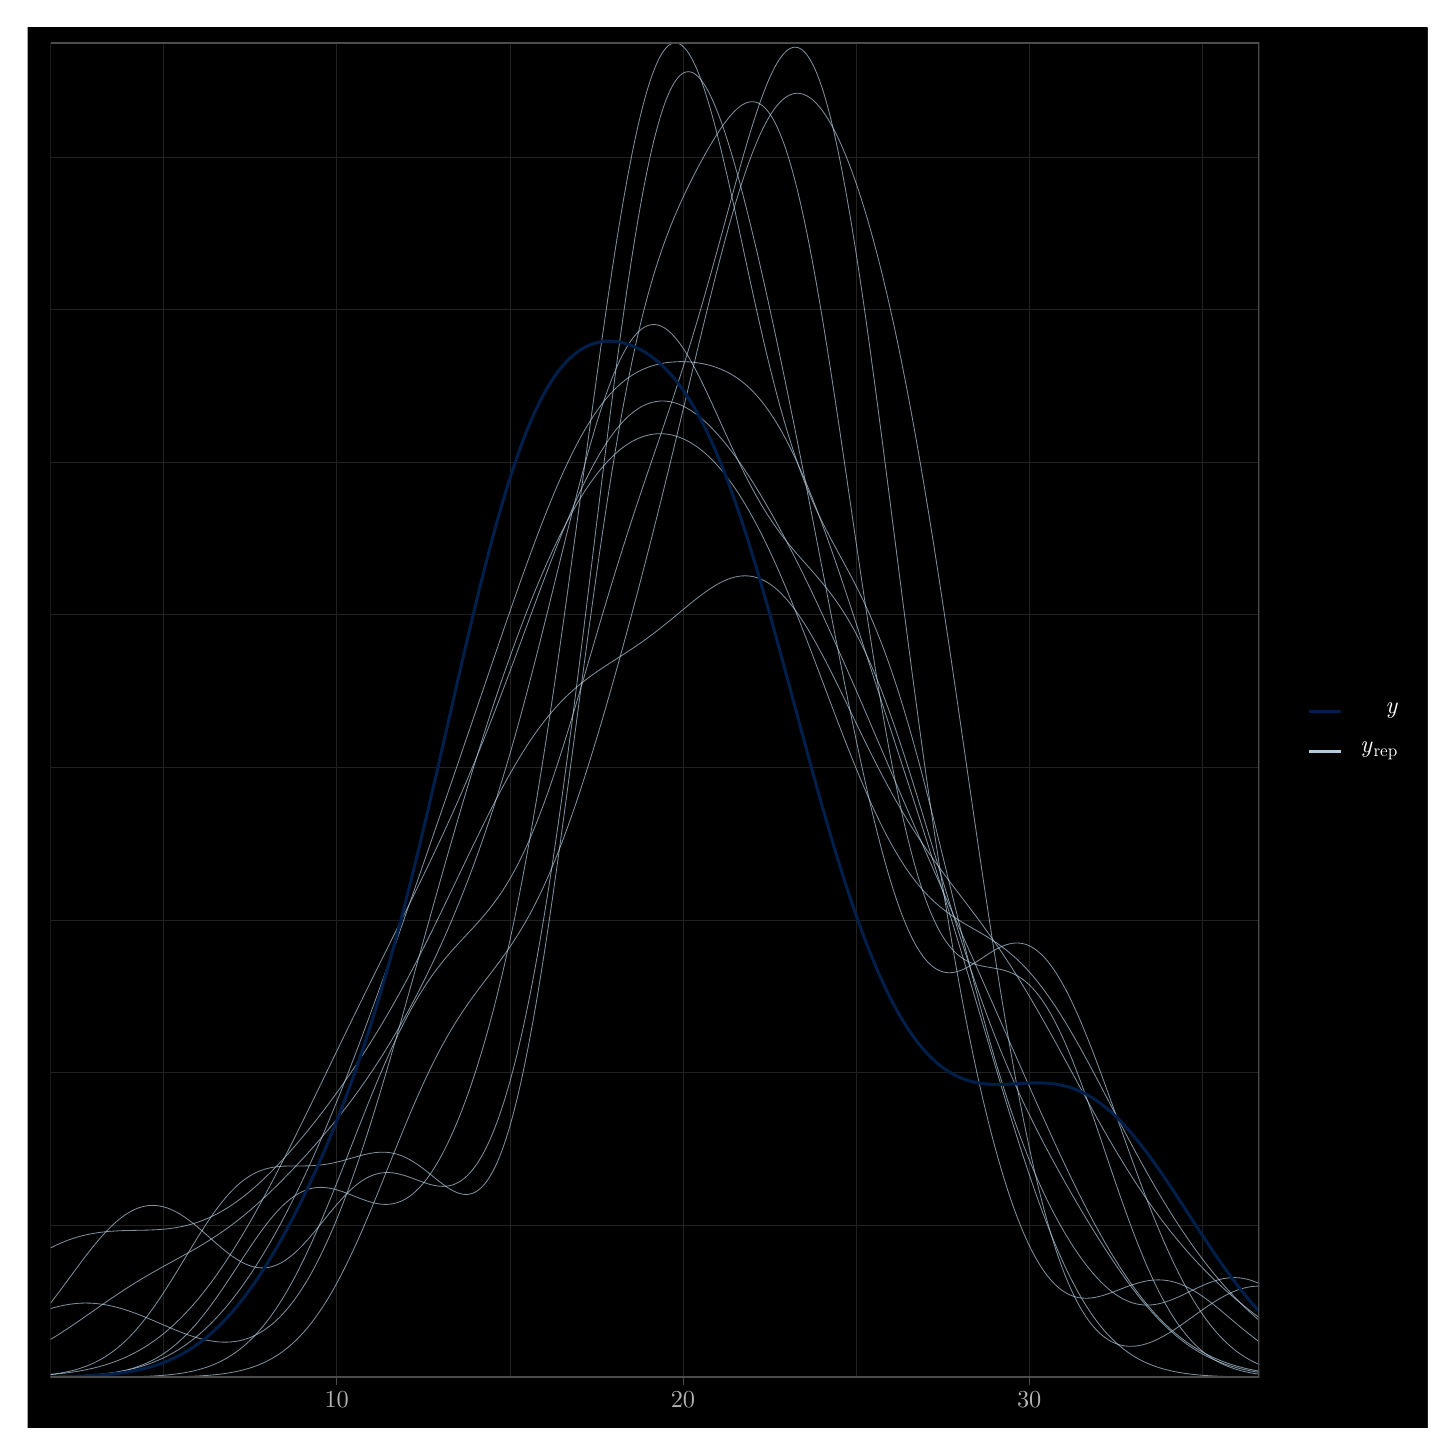
\begin{tikzpicture}[x=1pt,y=1pt]
\definecolor{fillColor}{RGB}{255,255,255}
\path[use as bounding box,fill=fillColor,fill opacity=0.00] (0,0) rectangle (505.89,505.89);
\begin{scope}
\path[clip] (  0.00,  0.00) rectangle (505.89,505.89);
\definecolor{drawColor}{RGB}{0,0,0}
\definecolor{fillColor}{RGB}{0,0,0}

\path[draw=drawColor,line width= 0.6pt,line join=round,line cap=round,fill=fillColor] (  0.00,  0.00) rectangle (505.89,505.89);
\end{scope}
\begin{scope}
\path[clip] (  8.25, 18.22) rectangle (445.03,500.39);
\definecolor{fillColor}{RGB}{0,0,0}

\path[fill=fillColor] (  8.25, 18.22) rectangle (445.03,500.39);
\definecolor{drawColor}{gray}{0.13}

\path[draw=drawColor,line width= 0.1pt,line join=round] (  8.25, 73.33) --
	(445.03, 73.33);

\path[draw=drawColor,line width= 0.1pt,line join=round] (  8.25,183.56) --
	(445.03,183.56);

\path[draw=drawColor,line width= 0.1pt,line join=round] (  8.25,293.79) --
	(445.03,293.79);

\path[draw=drawColor,line width= 0.1pt,line join=round] (  8.25,404.01) --
	(445.03,404.01);

\path[draw=drawColor,line width= 0.1pt,line join=round] ( 49.12, 18.22) --
	( 49.12,500.39);

\path[draw=drawColor,line width= 0.1pt,line join=round] (174.24, 18.22) --
	(174.24,500.39);

\path[draw=drawColor,line width= 0.1pt,line join=round] (299.35, 18.22) --
	(299.35,500.39);

\path[draw=drawColor,line width= 0.1pt,line join=round] (424.47, 18.22) --
	(424.47,500.39);

\path[draw=drawColor,line width= 0.3pt,line join=round] (  8.25,128.45) --
	(445.03,128.45);

\path[draw=drawColor,line width= 0.3pt,line join=round] (  8.25,238.67) --
	(445.03,238.67);

\path[draw=drawColor,line width= 0.3pt,line join=round] (  8.25,348.90) --
	(445.03,348.90);

\path[draw=drawColor,line width= 0.3pt,line join=round] (  8.25,459.13) --
	(445.03,459.13);

\path[draw=drawColor,line width= 0.3pt,line join=round] (111.68, 18.22) --
	(111.68,500.39);

\path[draw=drawColor,line width= 0.3pt,line join=round] (236.80, 18.22) --
	(236.80,500.39);

\path[draw=drawColor,line width= 0.3pt,line join=round] (361.91, 18.22) --
	(361.91,500.39);
\definecolor{drawColor}{RGB}{179,205,224}

\path[draw=drawColor,draw opacity=0.70,line width= 0.3pt,line join=round] (  8.25, 18.31) --
	(  8.68, 18.32) --
	(  9.10, 18.33) --
	(  9.53, 18.33) --
	(  9.96, 18.34) --
	( 10.38, 18.35) --
	( 10.81, 18.35) --
	( 11.24, 18.36) --
	( 11.67, 18.37) --
	( 12.09, 18.38) --
	( 12.52, 18.39) --
	( 12.95, 18.40) --
	( 13.37, 18.41) --
	( 13.80, 18.42) --
	( 14.23, 18.43) --
	( 14.65, 18.44) --
	( 15.08, 18.46) --
	( 15.51, 18.47) --
	( 15.94, 18.49) --
	( 16.36, 18.50) --
	( 16.79, 18.52) --
	( 17.22, 18.53) --
	( 17.64, 18.55) --
	( 18.07, 18.57) --
	( 18.50, 18.59) --
	( 18.92, 18.61) --
	( 19.35, 18.63) --
	( 19.78, 18.65) --
	( 20.20, 18.68) --
	( 20.63, 18.70) --
	( 21.06, 18.73) --
	( 21.49, 18.76) --
	( 21.91, 18.79) --
	( 22.34, 18.82) --
	( 22.77, 18.85) --
	( 23.19, 18.88) --
	( 23.62, 18.91) --
	( 24.05, 18.95) --
	( 24.47, 18.99) --
	( 24.90, 19.03) --
	( 25.33, 19.07) --
	( 25.76, 19.11) --
	( 26.18, 19.16) --
	( 26.61, 19.20) --
	( 27.04, 19.25) --
	( 27.46, 19.30) --
	( 27.89, 19.36) --
	( 28.32, 19.41) --
	( 28.74, 19.47) --
	( 29.17, 19.53) --
	( 29.60, 19.59) --
	( 30.02, 19.66) --
	( 30.45, 19.72) --
	( 30.88, 19.79) --
	( 31.31, 19.87) --
	( 31.73, 19.94) --
	( 32.16, 20.02) --
	( 32.59, 20.11) --
	( 33.01, 20.19) --
	( 33.44, 20.28) --
	( 33.87, 20.37) --
	( 34.29, 20.47) --
	( 34.72, 20.57) --
	( 35.15, 20.67) --
	( 35.58, 20.78) --
	( 36.00, 20.89) --
	( 36.43, 21.00) --
	( 36.86, 21.12) --
	( 37.28, 21.25) --
	( 37.71, 21.37) --
	( 38.14, 21.50) --
	( 38.56, 21.64) --
	( 38.99, 21.78) --
	( 39.42, 21.93) --
	( 39.84, 22.08) --
	( 40.27, 22.23) --
	( 40.70, 22.39) --
	( 41.13, 22.56) --
	( 41.55, 22.73) --
	( 41.98, 22.91) --
	( 42.41, 23.09) --
	( 42.83, 23.28) --
	( 43.26, 23.47) --
	( 43.69, 23.67) --
	( 44.11, 23.87) --
	( 44.54, 24.08) --
	( 44.97, 24.30) --
	( 45.40, 24.52) --
	( 45.82, 24.75) --
	( 46.25, 24.99) --
	( 46.68, 25.23) --
	( 47.10, 25.48) --
	( 47.53, 25.74) --
	( 47.96, 26.00) --
	( 48.38, 26.27) --
	( 48.81, 26.54) --
	( 49.24, 26.83) --
	( 49.66, 27.12) --
	( 50.09, 27.42) --
	( 50.52, 27.72) --
	( 50.95, 28.03) --
	( 51.37, 28.35) --
	( 51.80, 28.68) --
	( 52.23, 29.02) --
	( 52.65, 29.36) --
	( 53.08, 29.71) --
	( 53.51, 30.07) --
	( 53.93, 30.43) --
	( 54.36, 30.81) --
	( 54.79, 31.19) --
	( 55.22, 31.58) --
	( 55.64, 31.97) --
	( 56.07, 32.38) --
	( 56.50, 32.79) --
	( 56.92, 33.21) --
	( 57.35, 33.64) --
	( 57.78, 34.07) --
	( 58.20, 34.52) --
	( 58.63, 34.97) --
	( 59.06, 35.43) --
	( 59.48, 35.90) --
	( 59.91, 36.37) --
	( 60.34, 36.85) --
	( 60.77, 37.34) --
	( 61.19, 37.84) --
	( 61.62, 38.34) --
	( 62.05, 38.86) --
	( 62.47, 39.37) --
	( 62.90, 39.90) --
	( 63.33, 40.43) --
	( 63.75, 40.97) --
	( 64.18, 41.52) --
	( 64.61, 42.07) --
	( 65.04, 42.63) --
	( 65.46, 43.20) --
	( 65.89, 43.77) --
	( 66.32, 44.35) --
	( 66.74, 44.93) --
	( 67.17, 45.52) --
	( 67.60, 46.12) --
	( 68.02, 46.72) --
	( 68.45, 47.32) --
	( 68.88, 47.93) --
	( 69.30, 48.55) --
	( 69.73, 49.17) --
	( 70.16, 49.79) --
	( 70.59, 50.42) --
	( 71.01, 51.05) --
	( 71.44, 51.68) --
	( 71.87, 52.32) --
	( 72.29, 52.96) --
	( 72.72, 53.61) --
	( 73.15, 54.25) --
	( 73.57, 54.90) --
	( 74.00, 55.55) --
	( 74.43, 56.20) --
	( 74.86, 56.85) --
	( 75.28, 57.50) --
	( 75.71, 58.15) --
	( 76.14, 58.81) --
	( 76.56, 59.46) --
	( 76.99, 60.11) --
	( 77.42, 60.76) --
	( 77.84, 61.41) --
	( 78.27, 62.06) --
	( 78.70, 62.71) --
	( 79.12, 63.35) --
	( 79.55, 64.00) --
	( 79.98, 64.64) --
	( 80.41, 65.27) --
	( 80.83, 65.91) --
	( 81.26, 66.53) --
	( 81.69, 67.16) --
	( 82.11, 67.78) --
	( 82.54, 68.39) --
	( 82.97, 69.00) --
	( 83.39, 69.60) --
	( 83.82, 70.20) --
	( 84.25, 70.79) --
	( 84.68, 71.38) --
	( 85.10, 71.96) --
	( 85.53, 72.53) --
	( 85.96, 73.09) --
	( 86.38, 73.64) --
	( 86.81, 74.19) --
	( 87.24, 74.73) --
	( 87.66, 75.26) --
	( 88.09, 75.78) --
	( 88.52, 76.29) --
	( 88.94, 76.79) --
	( 89.37, 77.28) --
	( 89.80, 77.76) --
	( 90.23, 78.22) --
	( 90.65, 78.68) --
	( 91.08, 79.13) --
	( 91.51, 79.57) --
	( 91.93, 79.99) --
	( 92.36, 80.40) --
	( 92.79, 80.80) --
	( 93.21, 81.19) --
	( 93.64, 81.57) --
	( 94.07, 81.93) --
	( 94.49, 82.28) --
	( 94.92, 82.62) --
	( 95.35, 82.95) --
	( 95.78, 83.26) --
	( 96.20, 83.56) --
	( 96.63, 83.85) --
	( 97.06, 84.12) --
	( 97.48, 84.38) --
	( 97.91, 84.63) --
	( 98.34, 84.86) --
	( 98.76, 85.08) --
	( 99.19, 85.29) --
	( 99.62, 85.48) --
	(100.05, 85.66) --
	(100.47, 85.83) --
	(100.90, 85.98) --
	(101.33, 86.12) --
	(101.75, 86.25) --
	(102.18, 86.36) --
	(102.61, 86.46) --
	(103.03, 86.55) --
	(103.46, 86.63) --
	(103.89, 86.69) --
	(104.31, 86.74) --
	(104.74, 86.78) --
	(105.17, 86.80) --
	(105.60, 86.82) --
	(106.02, 86.83) --
	(106.45, 86.82) --
	(106.88, 86.80) --
	(107.30, 86.77) --
	(107.73, 86.73) --
	(108.16, 86.69) --
	(108.58, 86.63) --
	(109.01, 86.56) --
	(109.44, 86.48) --
	(109.87, 86.40) --
	(110.29, 86.31) --
	(110.72, 86.20) --
	(111.15, 86.09) --
	(111.57, 85.98) --
	(112.00, 85.86) --
	(112.43, 85.73) --
	(112.85, 85.59) --
	(113.28, 85.45) --
	(113.71, 85.30) --
	(114.13, 85.15) --
	(114.56, 85.00) --
	(114.99, 84.84) --
	(115.42, 84.68) --
	(115.84, 84.52) --
	(116.27, 84.35) --
	(116.70, 84.18) --
	(117.12, 84.01) --
	(117.55, 83.84) --
	(117.98, 83.67) --
	(118.40, 83.50) --
	(118.83, 83.33) --
	(119.26, 83.16) --
	(119.69, 82.99) --
	(120.11, 82.83) --
	(120.54, 82.67) --
	(120.97, 82.51) --
	(121.39, 82.35) --
	(121.82, 82.20) --
	(122.25, 82.05) --
	(122.67, 81.91) --
	(123.10, 81.77) --
	(123.53, 81.64) --
	(123.95, 81.51) --
	(124.38, 81.40) --
	(124.81, 81.29) --
	(125.24, 81.18) --
	(125.66, 81.09) --
	(126.09, 81.00) --
	(126.52, 80.93) --
	(126.94, 80.86) --
	(127.37, 80.80) --
	(127.80, 80.76) --
	(128.22, 80.72) --
	(128.65, 80.70) --
	(129.08, 80.68) --
	(129.51, 80.68) --
	(129.93, 80.69) --
	(130.36, 80.72) --
	(130.79, 80.75) --
	(131.21, 80.80) --
	(131.64, 80.87) --
	(132.07, 80.94) --
	(132.49, 81.03) --
	(132.92, 81.14) --
	(133.35, 81.26) --
	(133.77, 81.39) --
	(134.20, 81.55) --
	(134.63, 81.71) --
	(135.06, 81.89) --
	(135.48, 82.09) --
	(135.91, 82.31) --
	(136.34, 82.54) --
	(136.76, 82.79) --
	(137.19, 83.05) --
	(137.62, 83.33) --
	(138.04, 83.63) --
	(138.47, 83.95) --
	(138.90, 84.28) --
	(139.33, 84.62) --
	(139.75, 84.99) --
	(140.18, 85.38) --
	(140.61, 85.78) --
	(141.03, 86.20) --
	(141.46, 86.64) --
	(141.89, 87.10) --
	(142.31, 87.57) --
	(142.74, 88.06) --
	(143.17, 88.57) --
	(143.59, 89.10) --
	(144.02, 89.65) --
	(144.45, 90.21) --
	(144.88, 90.79) --
	(145.30, 91.40) --
	(145.73, 92.02) --
	(146.16, 92.65) --
	(146.58, 93.31) --
	(147.01, 93.99) --
	(147.44, 94.68) --
	(147.86, 95.39) --
	(148.29, 96.12) --
	(148.72, 96.86) --
	(149.15, 97.63) --
	(149.57, 98.41) --
	(150.00, 99.21) --
	(150.43,100.03) --
	(150.85,100.87) --
	(151.28,101.73) --
	(151.71,102.60) --
	(152.13,103.49) --
	(152.56,104.40) --
	(152.99,105.33) --
	(153.41,106.27) --
	(153.84,107.24) --
	(154.27,108.22) --
	(154.70,109.22) --
	(155.12,110.24) --
	(155.55,111.28) --
	(155.98,112.33) --
	(156.40,113.41) --
	(156.83,114.50) --
	(157.26,115.60) --
	(157.68,116.74) --
	(158.11,117.88) --
	(158.54,119.05) --
	(158.97,120.23) --
	(159.39,121.43) --
	(159.82,122.65) --
	(160.25,123.89) --
	(160.67,125.16) --
	(161.10,126.43) --
	(161.53,127.73) --
	(161.95,129.05) --
	(162.38,130.38) --
	(162.81,131.74) --
	(163.23,133.12) --
	(163.66,134.51) --
	(164.09,135.93) --
	(164.52,137.36) --
	(164.94,138.82) --
	(165.37,140.30) --
	(165.80,141.79) --
	(166.22,143.32) --
	(166.65,144.85) --
	(167.08,146.41) --
	(167.50,148.00) --
	(167.93,149.61) --
	(168.36,151.23) --
	(168.79,152.88) --
	(169.21,154.55) --
	(169.64,156.25) --
	(170.07,157.96) --
	(170.49,159.71) --
	(170.92,161.47) --
	(171.35,163.26) --
	(171.77,165.07) --
	(172.20,166.90) --
	(172.63,168.76) --
	(173.05,170.65) --
	(173.48,172.56) --
	(173.91,174.49) --
	(174.34,176.45) --
	(174.76,178.43) --
	(175.19,180.44) --
	(175.62,182.47) --
	(176.04,184.54) --
	(176.47,186.62) --
	(176.90,188.73) --
	(177.32,190.87) --
	(177.75,193.03) --
	(178.18,195.22) --
	(178.61,197.44) --
	(179.03,199.68) --
	(179.46,201.95) --
	(179.89,204.25) --
	(180.31,206.57) --
	(180.74,208.92) --
	(181.17,211.30) --
	(181.59,213.70) --
	(182.02,216.13) --
	(182.45,218.58) --
	(182.87,221.07) --
	(183.30,223.57) --
	(183.73,226.10) --
	(184.16,228.67) --
	(184.58,231.25) --
	(185.01,233.86) --
	(185.44,236.50) --
	(185.86,239.16) --
	(186.29,241.84) --
	(186.72,244.55) --
	(187.14,247.29) --
	(187.57,250.05) --
	(188.00,252.83) --
	(188.43,255.64) --
	(188.85,258.46) --
	(189.28,261.31) --
	(189.71,264.18) --
	(190.13,267.08) --
	(190.56,269.98) --
	(190.99,272.92) --
	(191.41,275.87) --
	(191.84,278.84) --
	(192.27,281.83) --
	(192.69,284.84) --
	(193.12,287.86) --
	(193.55,290.90) --
	(193.98,293.96) --
	(194.40,297.03) --
	(194.83,300.11) --
	(195.26,303.21) --
	(195.68,306.32) --
	(196.11,309.43) --
	(196.54,312.57) --
	(196.96,315.70) --
	(197.39,318.85) --
	(197.82,322.01) --
	(198.25,325.17) --
	(198.67,328.33) --
	(199.10,331.51) --
	(199.53,334.68) --
	(199.95,337.86) --
	(200.38,341.04) --
	(200.81,344.21) --
	(201.23,347.39) --
	(201.66,350.57) --
	(202.09,353.74) --
	(202.51,356.91) --
	(202.94,360.07) --
	(203.37,363.22) --
	(203.80,366.37) --
	(204.22,369.51) --
	(204.65,372.64) --
	(205.08,375.75) --
	(205.50,378.85) --
	(205.93,381.95) --
	(206.36,385.02) --
	(206.78,388.07) --
	(207.21,391.12) --
	(207.64,394.13) --
	(208.07,397.13) --
	(208.49,400.11) --
	(208.92,403.07) --
	(209.35,406.00) --
	(209.77,408.91) --
	(210.20,411.79) --
	(210.63,414.63) --
	(211.05,417.46) --
	(211.48,420.26) --
	(211.91,423.01) --
	(212.33,425.74) --
	(212.76,428.44) --
	(213.19,431.10) --
	(213.62,433.72) --
	(214.04,436.31) --
	(214.47,438.86) --
	(214.90,441.37) --
	(215.32,443.84) --
	(215.75,446.27) --
	(216.18,448.65) --
	(216.60,450.99) --
	(217.03,453.30) --
	(217.46,455.54) --
	(217.89,457.74) --
	(218.31,459.91) --
	(218.74,462.01) --
	(219.17,464.07) --
	(219.59,466.09) --
	(220.02,468.04) --
	(220.45,469.94) --
	(220.87,471.80) --
	(221.30,473.60) --
	(221.73,475.34) --
	(222.15,477.04) --
	(222.58,478.68) --
	(223.01,480.25) --
	(223.44,481.78) --
	(223.86,483.25) --
	(224.29,484.65) --
	(224.72,486.00) --
	(225.14,487.30) --
	(225.57,488.53) --
	(226.00,489.69) --
	(226.42,490.81) --
	(226.85,491.87) --
	(227.28,492.85) --
	(227.71,493.79) --
	(228.13,494.66) --
	(228.56,495.46) --
	(228.99,496.21) --
	(229.41,496.91) --
	(229.84,497.52) --
	(230.27,498.08) --
	(230.69,498.60) --
	(231.12,499.03) --
	(231.55,499.40) --
	(231.97,499.73) --
	(232.40,499.98) --
	(232.83,500.17) --
	(233.26,500.31) --
	(233.68,500.39) --
	(234.11,500.39) --
	(234.54,500.34) --
	(234.96,500.25) --
	(235.39,500.07) --
	(235.82,499.85) --
	(236.24,499.58) --
	(236.67,499.23) --
	(237.10,498.83) --
	(237.53,498.38) --
	(237.95,497.87) --
	(238.38,497.30) --
	(238.81,496.68) --
	(239.23,496.01) --
	(239.66,495.28) --
	(240.09,494.50) --
	(240.51,493.68) --
	(240.94,492.79) --
	(241.37,491.86) --
	(241.79,490.89) --
	(242.22,489.85) --
	(242.65,488.77) --
	(243.08,487.66) --
	(243.50,486.49) --
	(243.93,485.28) --
	(244.36,484.03) --
	(244.78,482.74) --
	(245.21,481.39) --
	(245.64,480.02) --
	(246.06,478.61) --
	(246.49,477.16) --
	(246.92,475.67) --
	(247.35,474.15) --
	(247.77,472.59) --
	(248.20,471.00) --
	(248.63,469.39) --
	(249.05,467.74) --
	(249.48,466.06) --
	(249.91,464.35) --
	(250.33,462.62) --
	(250.76,460.86) --
	(251.19,459.09) --
	(251.61,457.29) --
	(252.04,455.46) --
	(252.47,453.62) --
	(252.90,451.76) --
	(253.32,449.88) --
	(253.75,447.99) --
	(254.18,446.08) --
	(254.60,444.16) --
	(255.03,442.23) --
	(255.46,440.28) --
	(255.88,438.33) --
	(256.31,436.37) --
	(256.74,434.40) --
	(257.17,432.43) --
	(257.59,430.46) --
	(258.02,428.48) --
	(258.45,426.50) --
	(258.87,424.52) --
	(259.30,422.54) --
	(259.73,420.56) --
	(260.15,418.58) --
	(260.58,416.61) --
	(261.01,414.64) --
	(261.43,412.68) --
	(261.86,410.73) --
	(262.29,408.78) --
	(262.72,406.85) --
	(263.14,404.92) --
	(263.57,403.01) --
	(264.00,401.10) --
	(264.42,399.22) --
	(264.85,397.34) --
	(265.28,395.48) --
	(265.70,393.63) --
	(266.13,391.80) --
	(266.56,389.99) --
	(266.98,388.19) --
	(267.41,386.41) --
	(267.84,384.65) --
	(268.27,382.91) --
	(268.69,381.19) --
	(269.12,379.49) --
	(269.55,377.81) --
	(269.97,376.15) --
	(270.40,374.51) --
	(270.83,372.89) --
	(271.25,371.30) --
	(271.68,369.73) --
	(272.11,368.18) --
	(272.54,366.65) --
	(272.96,365.15) --
	(273.39,363.67) --
	(273.82,362.20) --
	(274.24,360.77) --
	(274.67,359.36) --
	(275.10,357.97) --
	(275.52,356.61) --
	(275.95,355.26) --
	(276.38,353.94) --
	(276.80,352.64) --
	(277.23,351.37) --
	(277.66,350.12) --
	(278.09,348.88) --
	(278.51,347.68) --
	(278.94,346.49) --
	(279.37,345.32) --
	(279.79,344.17) --
	(280.22,343.05) --
	(280.65,341.94) --
	(281.07,340.85) --
	(281.50,339.79) --
	(281.93,338.74) --
	(282.36,337.71) --
	(282.78,336.69) --
	(283.21,335.69) --
	(283.64,334.71) --
	(284.06,333.75) --
	(284.49,332.80) --
	(284.92,331.86) --
	(285.34,330.94) --
	(285.77,330.04) --
	(286.20,329.14) --
	(286.62,328.26) --
	(287.05,327.39) --
	(287.48,326.52) --
	(287.91,325.67) --
	(288.33,324.83) --
	(288.76,324.00) --
	(289.19,323.17) --
	(289.61,322.36) --
	(290.04,321.55) --
	(290.47,320.74) --
	(290.89,319.94) --
	(291.32,319.14) --
	(291.75,318.35) --
	(292.18,317.56) --
	(292.60,316.78) --
	(293.03,315.99) --
	(293.46,315.21) --
	(293.88,314.42) --
	(294.31,313.64) --
	(294.74,312.85) --
	(295.16,312.06) --
	(295.59,311.27) --
	(296.02,310.48) --
	(296.44,309.68) --
	(296.87,308.88) --
	(297.30,308.08) --
	(297.73,307.27) --
	(298.15,306.45) --
	(298.58,305.63) --
	(299.01,304.79) --
	(299.43,303.95) --
	(299.86,303.11) --
	(300.29,302.25) --
	(300.71,301.39) --
	(301.14,300.51) --
	(301.57,299.63) --
	(302.00,298.73) --
	(302.42,297.82) --
	(302.85,296.91) --
	(303.28,295.98) --
	(303.70,295.03) --
	(304.13,294.08) --
	(304.56,293.11) --
	(304.98,292.13) --
	(305.41,291.13) --
	(305.84,290.12) --
	(306.26,289.10) --
	(306.69,288.06) --
	(307.12,287.01) --
	(307.55,285.94) --
	(307.97,284.86) --
	(308.40,283.76) --
	(308.83,282.65) --
	(309.25,281.52) --
	(309.68,280.37) --
	(310.11,279.21) --
	(310.53,278.03) --
	(310.96,276.84) --
	(311.39,275.63) --
	(311.82,274.41) --
	(312.24,273.16) --
	(312.67,271.91) --
	(313.10,270.63) --
	(313.52,269.34) --
	(313.95,268.04) --
	(314.38,266.71) --
	(314.80,265.38) --
	(315.23,264.02) --
	(315.66,262.65) --
	(316.08,261.27) --
	(316.51,259.87) --
	(316.94,258.45) --
	(317.37,257.02) --
	(317.79,255.57) --
	(318.22,254.11) --
	(318.65,252.64) --
	(319.07,251.15) --
	(319.50,249.65) --
	(319.93,248.13) --
	(320.35,246.60) --
	(320.78,245.05) --
	(321.21,243.50) --
	(321.64,241.93) --
	(322.06,240.35) --
	(322.49,238.75) --
	(322.92,237.15) --
	(323.34,235.53) --
	(323.77,233.91) --
	(324.20,232.27) --
	(324.62,230.62) --
	(325.05,228.97) --
	(325.48,227.30) --
	(325.90,225.63) --
	(326.33,223.94) --
	(326.76,222.25) --
	(327.19,220.56) --
	(327.61,218.85) --
	(328.04,217.14) --
	(328.47,215.42) --
	(328.89,213.70) --
	(329.32,211.97) --
	(329.75,210.24) --
	(330.17,208.50) --
	(330.60,206.76) --
	(331.03,205.02) --
	(331.46,203.28) --
	(331.88,201.53) --
	(332.31,199.78) --
	(332.74,198.03) --
	(333.16,196.28) --
	(333.59,194.52) --
	(334.02,192.77) --
	(334.44,191.02) --
	(334.87,189.27) --
	(335.30,187.53) --
	(335.72,185.78) --
	(336.15,184.04) --
	(336.58,182.30) --
	(337.01,180.56) --
	(337.43,178.83) --
	(337.86,177.10) --
	(338.29,175.38) --
	(338.71,173.67) --
	(339.14,171.95) --
	(339.57,170.25) --
	(339.99,168.55) --
	(340.42,166.86) --
	(340.85,165.18) --
	(341.28,163.50) --
	(341.70,161.84) --
	(342.13,160.18) --
	(342.56,158.53) --
	(342.98,156.89) --
	(343.41,155.26) --
	(343.84,153.64) --
	(344.26,152.03) --
	(344.69,150.43) --
	(345.12,148.85) --
	(345.54,147.27) --
	(345.97,145.70) --
	(346.40,144.15) --
	(346.83,142.61) --
	(347.25,141.08) --
	(347.68,139.57) --
	(348.11,138.06) --
	(348.53,136.57) --
	(348.96,135.09) --
	(349.39,133.63) --
	(349.81,132.18) --
	(350.24,130.74) --
	(350.67,129.32) --
	(351.10,127.91) --
	(351.52,126.51) --
	(351.95,125.13) --
	(352.38,123.76) --
	(352.80,122.40) --
	(353.23,121.06) --
	(353.66,119.74) --
	(354.08,118.42) --
	(354.51,117.12) --
	(354.94,115.84) --
	(355.36,114.57) --
	(355.79,113.31) --
	(356.22,112.07) --
	(356.65,110.84) --
	(357.07,109.63) --
	(357.50,108.43) --
	(357.93,107.25) --
	(358.35,106.07) --
	(358.78,104.92) --
	(359.21,103.77) --
	(359.63,102.64) --
	(360.06,101.52) --
	(360.49,100.42) --
	(360.92, 99.33) --
	(361.34, 98.25) --
	(361.77, 97.19) --
	(362.20, 96.13) --
	(362.62, 95.09) --
	(363.05, 94.07) --
	(363.48, 93.05) --
	(363.90, 92.05) --
	(364.33, 91.06) --
	(364.76, 90.09) --
	(365.18, 89.12) --
	(365.61, 88.17) --
	(366.04, 87.23) --
	(366.47, 86.30) --
	(366.89, 85.38) --
	(367.32, 84.47) --
	(367.75, 83.58) --
	(368.17, 82.69) --
	(368.60, 81.82) --
	(369.03, 80.96) --
	(369.45, 80.10) --
	(369.88, 79.26) --
	(370.31, 78.43) --
	(370.74, 77.61) --
	(371.16, 76.80) --
	(371.59, 76.00) --
	(372.02, 75.21) --
	(372.44, 74.43) --
	(372.87, 73.66) --
	(373.30, 72.90) --
	(373.72, 72.15) --
	(374.15, 71.41) --
	(374.58, 70.68) --
	(375.00, 69.95) --
	(375.43, 69.24) --
	(375.86, 68.54) --
	(376.29, 67.84) --
	(376.71, 67.16) --
	(377.14, 66.49) --
	(377.57, 65.82) --
	(377.99, 65.16) --
	(378.42, 64.52) --
	(378.85, 63.88) --
	(379.27, 63.25) --
	(379.70, 62.63) --
	(380.13, 62.02) --
	(380.56, 61.42) --
	(380.98, 60.83) --
	(381.41, 60.25) --
	(381.84, 59.68) --
	(382.26, 59.12) --
	(382.69, 58.56) --
	(383.12, 58.02) --
	(383.54, 57.48) --
	(383.97, 56.96) --
	(384.40, 56.45) --
	(384.82, 55.94) --
	(385.25, 55.45) --
	(385.68, 54.96) --
	(386.11, 54.48) --
	(386.53, 54.02) --
	(386.96, 53.57) --
	(387.39, 53.12) --
	(387.81, 52.69) --
	(388.24, 52.26) --
	(388.67, 51.85) --
	(389.09, 51.45) --
	(389.52, 51.05) --
	(389.95, 50.67) --
	(390.38, 50.30) --
	(390.80, 49.94) --
	(391.23, 49.59) --
	(391.66, 49.25) --
	(392.08, 48.93) --
	(392.51, 48.61) --
	(392.94, 48.30) --
	(393.36, 48.01) --
	(393.79, 47.73) --
	(394.22, 47.45) --
	(394.64, 47.19) --
	(395.07, 46.94) --
	(395.50, 46.70) --
	(395.93, 46.48) --
	(396.35, 46.26) --
	(396.78, 46.06) --
	(397.21, 45.87) --
	(397.63, 45.69) --
	(398.06, 45.52) --
	(398.49, 45.36) --
	(398.91, 45.21) --
	(399.34, 45.08) --
	(399.77, 44.95) --
	(400.20, 44.84) --
	(400.62, 44.74) --
	(401.05, 44.64) --
	(401.48, 44.56) --
	(401.90, 44.50) --
	(402.33, 44.44) --
	(402.76, 44.39) --
	(403.18, 44.35) --
	(403.61, 44.33) --
	(404.04, 44.31) --
	(404.46, 44.31) --
	(404.89, 44.31) --
	(405.32, 44.32) --
	(405.75, 44.35) --
	(406.17, 44.38) --
	(406.60, 44.43) --
	(407.03, 44.48) --
	(407.45, 44.54) --
	(407.88, 44.61) --
	(408.31, 44.69) --
	(408.73, 44.78) --
	(409.16, 44.88) --
	(409.59, 44.98) --
	(410.02, 45.09) --
	(410.44, 45.21) --
	(410.87, 45.34) --
	(411.30, 45.47) --
	(411.72, 45.61) --
	(412.15, 45.76) --
	(412.58, 45.91) --
	(413.00, 46.07) --
	(413.43, 46.23) --
	(413.86, 46.40) --
	(414.28, 46.58) --
	(414.71, 46.76) --
	(415.14, 46.94) --
	(415.57, 47.13) --
	(415.99, 47.32) --
	(416.42, 47.51) --
	(416.85, 47.71) --
	(417.27, 47.91) --
	(417.70, 48.11) --
	(418.13, 48.31) --
	(418.55, 48.52) --
	(418.98, 48.72) --
	(419.41, 48.93) --
	(419.84, 49.14) --
	(420.26, 49.34) --
	(420.69, 49.55) --
	(421.12, 49.76) --
	(421.54, 49.96) --
	(421.97, 50.17) --
	(422.40, 50.37) --
	(422.82, 50.57) --
	(423.25, 50.77) --
	(423.68, 50.97) --
	(424.10, 51.16) --
	(424.53, 51.35) --
	(424.96, 51.54) --
	(425.39, 51.72) --
	(425.81, 51.90) --
	(426.24, 52.07) --
	(426.67, 52.24) --
	(427.09, 52.40) --
	(427.52, 52.56) --
	(427.95, 52.71) --
	(428.37, 52.86) --
	(428.80, 53.00) --
	(429.23, 53.14) --
	(429.66, 53.26) --
	(430.08, 53.38) --
	(430.51, 53.50) --
	(430.94, 53.60) --
	(431.36, 53.70) --
	(431.79, 53.79) --
	(432.22, 53.87) --
	(432.64, 53.94) --
	(433.07, 54.01) --
	(433.50, 54.07) --
	(433.92, 54.11) --
	(434.35, 54.15) --
	(434.78, 54.18) --
	(435.21, 54.20) --
	(435.63, 54.22) --
	(436.06, 54.22) --
	(436.49, 54.21) --
	(436.91, 54.20) --
	(437.34, 54.17) --
	(437.77, 54.13) --
	(438.19, 54.09) --
	(438.62, 54.04) --
	(439.05, 53.97) --
	(439.47, 53.89) --
	(439.90, 53.81) --
	(440.33, 53.72) --
	(440.76, 53.61) --
	(441.18, 53.50) --
	(441.61, 53.38) --
	(442.04, 53.25) --
	(442.46, 53.10) --
	(442.89, 52.96) --
	(443.32, 52.79) --
	(443.74, 52.62) --
	(444.17, 52.45) --
	(444.60, 52.26) --
	(445.03, 52.06);

\path[draw=drawColor,draw opacity=0.70,line width= 0.3pt,line join=round] (  8.25, 19.19) --
	(  8.68, 19.23) --
	(  9.10, 19.26) --
	(  9.53, 19.30) --
	(  9.96, 19.34) --
	( 10.38, 19.38) --
	( 10.81, 19.42) --
	( 11.24, 19.47) --
	( 11.67, 19.51) --
	( 12.09, 19.56) --
	( 12.52, 19.61) --
	( 12.95, 19.66) --
	( 13.37, 19.71) --
	( 13.80, 19.76) --
	( 14.23, 19.82) --
	( 14.65, 19.87) --
	( 15.08, 19.93) --
	( 15.51, 19.99) --
	( 15.94, 20.05) --
	( 16.36, 20.11) --
	( 16.79, 20.18) --
	( 17.22, 20.24) --
	( 17.64, 20.31) --
	( 18.07, 20.38) --
	( 18.50, 20.45) --
	( 18.92, 20.53) --
	( 19.35, 20.60) --
	( 19.78, 20.68) --
	( 20.20, 20.76) --
	( 20.63, 20.85) --
	( 21.06, 20.93) --
	( 21.49, 21.02) --
	( 21.91, 21.11) --
	( 22.34, 21.20) --
	( 22.77, 21.30) --
	( 23.19, 21.39) --
	( 23.62, 21.49) --
	( 24.05, 21.60) --
	( 24.47, 21.70) --
	( 24.90, 21.81) --
	( 25.33, 21.92) --
	( 25.76, 22.03) --
	( 26.18, 22.15) --
	( 26.61, 22.27) --
	( 27.04, 22.39) --
	( 27.46, 22.52) --
	( 27.89, 22.64) --
	( 28.32, 22.77) --
	( 28.74, 22.91) --
	( 29.17, 23.05) --
	( 29.60, 23.19) --
	( 30.02, 23.33) --
	( 30.45, 23.48) --
	( 30.88, 23.63) --
	( 31.31, 23.79) --
	( 31.73, 23.94) --
	( 32.16, 24.10) --
	( 32.59, 24.27) --
	( 33.01, 24.44) --
	( 33.44, 24.61) --
	( 33.87, 24.79) --
	( 34.29, 24.97) --
	( 34.72, 25.15) --
	( 35.15, 25.34) --
	( 35.58, 25.53) --
	( 36.00, 25.73) --
	( 36.43, 25.93) --
	( 36.86, 26.13) --
	( 37.28, 26.34) --
	( 37.71, 26.55) --
	( 38.14, 26.77) --
	( 38.56, 26.99) --
	( 38.99, 27.22) --
	( 39.42, 27.45) --
	( 39.84, 27.68) --
	( 40.27, 27.92) --
	( 40.70, 28.17) --
	( 41.13, 28.42) --
	( 41.55, 28.67) --
	( 41.98, 28.93) --
	( 42.41, 29.19) --
	( 42.83, 29.46) --
	( 43.26, 29.73) --
	( 43.69, 30.01) --
	( 44.11, 30.29) --
	( 44.54, 30.58) --
	( 44.97, 30.87) --
	( 45.40, 31.17) --
	( 45.82, 31.47) --
	( 46.25, 31.78) --
	( 46.68, 32.09) --
	( 47.10, 32.41) --
	( 47.53, 32.73) --
	( 47.96, 33.06) --
	( 48.38, 33.40) --
	( 48.81, 33.74) --
	( 49.24, 34.08) --
	( 49.66, 34.43) --
	( 50.09, 34.79) --
	( 50.52, 35.15) --
	( 50.95, 35.52) --
	( 51.37, 35.89) --
	( 51.80, 36.26) --
	( 52.23, 36.65) --
	( 52.65, 37.04) --
	( 53.08, 37.43) --
	( 53.51, 37.83) --
	( 53.93, 38.24) --
	( 54.36, 38.65) --
	( 54.79, 39.07) --
	( 55.22, 39.49) --
	( 55.64, 39.92) --
	( 56.07, 40.35) --
	( 56.50, 40.80) --
	( 56.92, 41.24) --
	( 57.35, 41.69) --
	( 57.78, 42.15) --
	( 58.20, 42.62) --
	( 58.63, 43.08) --
	( 59.06, 43.56) --
	( 59.48, 44.04) --
	( 59.91, 44.53) --
	( 60.34, 45.02) --
	( 60.77, 45.52) --
	( 61.19, 46.02) --
	( 61.62, 46.53) --
	( 62.05, 47.05) --
	( 62.47, 47.57) --
	( 62.90, 48.10) --
	( 63.33, 48.63) --
	( 63.75, 49.17) --
	( 64.18, 49.72) --
	( 64.61, 50.27) --
	( 65.04, 50.82) --
	( 65.46, 51.38) --
	( 65.89, 51.95) --
	( 66.32, 52.53) --
	( 66.74, 53.10) --
	( 67.17, 53.69) --
	( 67.60, 54.28) --
	( 68.02, 54.87) --
	( 68.45, 55.48) --
	( 68.88, 56.08) --
	( 69.30, 56.70) --
	( 69.73, 57.31) --
	( 70.16, 57.94) --
	( 70.59, 58.57) --
	( 71.01, 59.20) --
	( 71.44, 59.84) --
	( 71.87, 60.48) --
	( 72.29, 61.13) --
	( 72.72, 61.79) --
	( 73.15, 62.45) --
	( 73.57, 63.11) --
	( 74.00, 63.78) --
	( 74.43, 64.46) --
	( 74.86, 65.14) --
	( 75.28, 65.82) --
	( 75.71, 66.51) --
	( 76.14, 67.21) --
	( 76.56, 67.91) --
	( 76.99, 68.61) --
	( 77.42, 69.32) --
	( 77.84, 70.04) --
	( 78.27, 70.76) --
	( 78.70, 71.48) --
	( 79.12, 72.21) --
	( 79.55, 72.94) --
	( 79.98, 73.68) --
	( 80.41, 74.42) --
	( 80.83, 75.16) --
	( 81.26, 75.91) --
	( 81.69, 76.66) --
	( 82.11, 77.42) --
	( 82.54, 78.18) --
	( 82.97, 78.95) --
	( 83.39, 79.72) --
	( 83.82, 80.49) --
	( 84.25, 81.27) --
	( 84.68, 82.05) --
	( 85.10, 82.83) --
	( 85.53, 83.62) --
	( 85.96, 84.41) --
	( 86.38, 85.21) --
	( 86.81, 86.01) --
	( 87.24, 86.81) --
	( 87.66, 87.61) --
	( 88.09, 88.42) --
	( 88.52, 89.23) --
	( 88.94, 90.05) --
	( 89.37, 90.86) --
	( 89.80, 91.68) --
	( 90.23, 92.51) --
	( 90.65, 93.33) --
	( 91.08, 94.16) --
	( 91.51, 94.99) --
	( 91.93, 95.83) --
	( 92.36, 96.66) --
	( 92.79, 97.50) --
	( 93.21, 98.34) --
	( 93.64, 99.19) --
	( 94.07,100.03) --
	( 94.49,100.88) --
	( 94.92,101.73) --
	( 95.35,102.58) --
	( 95.78,103.44) --
	( 96.20,104.29) --
	( 96.63,105.15) --
	( 97.06,106.01) --
	( 97.48,106.87) --
	( 97.91,107.73) --
	( 98.34,108.60) --
	( 98.76,109.46) --
	( 99.19,110.33) --
	( 99.62,111.20) --
	(100.05,112.07) --
	(100.47,112.94) --
	(100.90,113.81) --
	(101.33,114.68) --
	(101.75,115.56) --
	(102.18,116.43) --
	(102.61,117.31) --
	(103.03,118.18) --
	(103.46,119.06) --
	(103.89,119.94) --
	(104.31,120.82) --
	(104.74,121.70) --
	(105.17,122.58) --
	(105.60,123.46) --
	(106.02,124.34) --
	(106.45,125.22) --
	(106.88,126.10) --
	(107.30,126.98) --
	(107.73,127.86) --
	(108.16,128.74) --
	(108.58,129.63) --
	(109.01,130.51) --
	(109.44,131.39) --
	(109.87,132.27) --
	(110.29,133.16) --
	(110.72,134.04) --
	(111.15,134.92) --
	(111.57,135.80) --
	(112.00,136.68) --
	(112.43,137.56) --
	(112.85,138.44) --
	(113.28,139.32) --
	(113.71,140.20) --
	(114.13,141.08) --
	(114.56,141.96) --
	(114.99,142.84) --
	(115.42,143.72) --
	(115.84,144.59) --
	(116.27,145.47) --
	(116.70,146.35) --
	(117.12,147.22) --
	(117.55,148.10) --
	(117.98,148.97) --
	(118.40,149.84) --
	(118.83,150.72) --
	(119.26,151.59) --
	(119.69,152.46) --
	(120.11,153.33) --
	(120.54,154.20) --
	(120.97,155.07) --
	(121.39,155.94) --
	(121.82,156.81) --
	(122.25,157.67) --
	(122.67,158.54) --
	(123.10,159.41) --
	(123.53,160.27) --
	(123.95,161.14) --
	(124.38,162.00) --
	(124.81,162.86) --
	(125.24,163.72) --
	(125.66,164.59) --
	(126.09,165.45) --
	(126.52,166.31) --
	(126.94,167.17) --
	(127.37,168.03) --
	(127.80,168.89) --
	(128.22,169.74) --
	(128.65,170.60) --
	(129.08,171.46) --
	(129.51,172.32) --
	(129.93,173.17) --
	(130.36,174.03) --
	(130.79,174.89) --
	(131.21,175.74) --
	(131.64,176.60) --
	(132.07,177.46) --
	(132.49,178.31) --
	(132.92,179.17) --
	(133.35,180.03) --
	(133.77,180.88) --
	(134.20,181.74) --
	(134.63,182.60) --
	(135.06,183.45) --
	(135.48,184.31) --
	(135.91,185.17) --
	(136.34,186.03) --
	(136.76,186.89) --
	(137.19,187.75) --
	(137.62,188.61) --
	(138.04,189.47) --
	(138.47,190.33) --
	(138.90,191.20) --
	(139.33,192.06) --
	(139.75,192.93) --
	(140.18,193.80) --
	(140.61,194.67) --
	(141.03,195.54) --
	(141.46,196.41) --
	(141.89,197.28) --
	(142.31,198.16) --
	(142.74,199.03) --
	(143.17,199.91) --
	(143.59,200.79) --
	(144.02,201.68) --
	(144.45,202.56) --
	(144.88,203.45) --
	(145.30,204.34) --
	(145.73,205.23) --
	(146.16,206.12) --
	(146.58,207.02) --
	(147.01,207.92) --
	(147.44,208.82) --
	(147.86,209.73) --
	(148.29,210.64) --
	(148.72,211.55) --
	(149.15,212.46) --
	(149.57,213.38) --
	(150.00,214.30) --
	(150.43,215.22) --
	(150.85,216.15) --
	(151.28,217.08) --
	(151.71,218.02) --
	(152.13,218.95) --
	(152.56,219.90) --
	(152.99,220.84) --
	(153.41,221.79) --
	(153.84,222.74) --
	(154.27,223.70) --
	(154.70,224.66) --
	(155.12,225.63) --
	(155.55,226.60) --
	(155.98,227.57) --
	(156.40,228.55) --
	(156.83,229.53) --
	(157.26,230.52) --
	(157.68,231.51) --
	(158.11,232.50) --
	(158.54,233.50) --
	(158.97,234.50) --
	(159.39,235.51) --
	(159.82,236.53) --
	(160.25,237.54) --
	(160.67,238.57) --
	(161.10,239.59) --
	(161.53,240.62) --
	(161.95,241.66) --
	(162.38,242.70) --
	(162.81,243.74) --
	(163.23,244.79) --
	(163.66,245.84) --
	(164.09,246.90) --
	(164.52,247.96) --
	(164.94,249.03) --
	(165.37,250.10) --
	(165.80,251.17) --
	(166.22,252.25) --
	(166.65,253.34) --
	(167.08,254.42) --
	(167.50,255.52) --
	(167.93,256.61) --
	(168.36,257.71) --
	(168.79,258.81) --
	(169.21,259.92) --
	(169.64,261.03) --
	(170.07,262.14) --
	(170.49,263.26) --
	(170.92,264.38) --
	(171.35,265.51) --
	(171.77,266.63) --
	(172.20,267.76) --
	(172.63,268.90) --
	(173.05,270.03) --
	(173.48,271.17) --
	(173.91,272.31) --
	(174.34,273.46) --
	(174.76,274.60) --
	(175.19,275.75) --
	(175.62,276.90) --
	(176.04,278.05) --
	(176.47,279.20) --
	(176.90,280.35) --
	(177.32,281.51) --
	(177.75,282.67) --
	(178.18,283.82) --
	(178.61,284.98) --
	(179.03,286.14) --
	(179.46,287.30) --
	(179.89,288.46) --
	(180.31,289.61) --
	(180.74,290.77) --
	(181.17,291.93) --
	(181.59,293.09) --
	(182.02,294.24) --
	(182.45,295.40) --
	(182.87,296.55) --
	(183.30,297.70) --
	(183.73,298.85) --
	(184.16,300.00) --
	(184.58,301.15) --
	(185.01,302.29) --
	(185.44,303.43) --
	(185.86,304.57) --
	(186.29,305.70) --
	(186.72,306.83) --
	(187.14,307.96) --
	(187.57,309.09) --
	(188.00,310.21) --
	(188.43,311.32) --
	(188.85,312.43) --
	(189.28,313.54) --
	(189.71,314.64) --
	(190.13,315.73) --
	(190.56,316.82) --
	(190.99,317.91) --
	(191.41,318.99) --
	(191.84,320.06) --
	(192.27,321.12) --
	(192.69,322.18) --
	(193.12,323.23) --
	(193.55,324.28) --
	(193.98,325.32) --
	(194.40,326.35) --
	(194.83,327.37) --
	(195.26,328.38) --
	(195.68,329.39) --
	(196.11,330.39) --
	(196.54,331.38) --
	(196.96,332.36) --
	(197.39,333.33) --
	(197.82,334.29) --
	(198.25,335.24) --
	(198.67,336.19) --
	(199.10,337.12) --
	(199.53,338.04) --
	(199.95,338.95) --
	(200.38,339.85) --
	(200.81,340.75) --
	(201.23,341.63) --
	(201.66,342.49) --
	(202.09,343.36) --
	(202.51,344.20) --
	(202.94,345.04) --
	(203.37,345.86) --
	(203.80,346.67) --
	(204.22,347.47) --
	(204.65,348.26) --
	(205.08,349.04) --
	(205.50,349.80) --
	(205.93,350.55) --
	(206.36,351.29) --
	(206.78,352.02) --
	(207.21,352.73) --
	(207.64,353.43) --
	(208.07,354.12) --
	(208.49,354.80) --
	(208.92,355.46) --
	(209.35,356.11) --
	(209.77,356.74) --
	(210.20,357.36) --
	(210.63,357.97) --
	(211.05,358.56) --
	(211.48,359.15) --
	(211.91,359.71) --
	(212.33,360.26) --
	(212.76,360.80) --
	(213.19,361.33) --
	(213.62,361.84) --
	(214.04,362.34) --
	(214.47,362.82) --
	(214.90,363.29) --
	(215.32,363.74) --
	(215.75,364.19) --
	(216.18,364.62) --
	(216.60,365.03) --
	(217.03,365.43) --
	(217.46,365.81) --
	(217.89,366.18) --
	(218.31,366.54) --
	(218.74,366.88) --
	(219.17,367.21) --
	(219.59,367.53) --
	(220.02,367.82) --
	(220.45,368.11) --
	(220.87,368.38) --
	(221.30,368.64) --
	(221.73,368.89) --
	(222.15,369.12) --
	(222.58,369.33) --
	(223.01,369.54) --
	(223.44,369.73) --
	(223.86,369.90) --
	(224.29,370.07) --
	(224.72,370.21) --
	(225.14,370.35) --
	(225.57,370.47) --
	(226.00,370.58) --
	(226.42,370.68) --
	(226.85,370.76) --
	(227.28,370.83) --
	(227.71,370.89) --
	(228.13,370.93) --
	(228.56,370.96) --
	(228.99,370.98) --
	(229.41,370.98) --
	(229.84,370.97) --
	(230.27,370.95) --
	(230.69,370.92) --
	(231.12,370.87) --
	(231.55,370.82) --
	(231.97,370.75) --
	(232.40,370.67) --
	(232.83,370.57) --
	(233.26,370.47) --
	(233.68,370.35) --
	(234.11,370.22) --
	(234.54,370.08) --
	(234.96,369.93) --
	(235.39,369.77) --
	(235.82,369.60) --
	(236.24,369.41) --
	(236.67,369.21) --
	(237.10,369.01) --
	(237.53,368.79) --
	(237.95,368.56) --
	(238.38,368.32) --
	(238.81,368.07) --
	(239.23,367.81) --
	(239.66,367.54) --
	(240.09,367.26) --
	(240.51,366.97) --
	(240.94,366.67) --
	(241.37,366.36) --
	(241.79,366.04) --
	(242.22,365.71) --
	(242.65,365.37) --
	(243.08,365.03) --
	(243.50,364.67) --
	(243.93,364.30) --
	(244.36,363.93) --
	(244.78,363.54) --
	(245.21,363.15) --
	(245.64,362.75) --
	(246.06,362.33) --
	(246.49,361.92) --
	(246.92,361.49) --
	(247.35,361.05) --
	(247.77,360.61) --
	(248.20,360.15) --
	(248.63,359.69) --
	(249.05,359.22) --
	(249.48,358.75) --
	(249.91,358.26) --
	(250.33,357.77) --
	(250.76,357.27) --
	(251.19,356.77) --
	(251.61,356.25) --
	(252.04,355.73) --
	(252.47,355.20) --
	(252.90,354.66) --
	(253.32,354.12) --
	(253.75,353.57) --
	(254.18,353.01) --
	(254.60,352.45) --
	(255.03,351.87) --
	(255.46,351.30) --
	(255.88,350.71) --
	(256.31,350.12) --
	(256.74,349.52) --
	(257.17,348.92) --
	(257.59,348.31) --
	(258.02,347.69) --
	(258.45,347.07) --
	(258.87,346.44) --
	(259.30,345.81) --
	(259.73,345.17) --
	(260.15,344.52) --
	(260.58,343.87) --
	(261.01,343.21) --
	(261.43,342.55) --
	(261.86,341.88) --
	(262.29,341.20) --
	(262.72,340.52) --
	(263.14,339.83) --
	(263.57,339.14) --
	(264.00,338.45) --
	(264.42,337.74) --
	(264.85,337.04) --
	(265.28,336.32) --
	(265.70,335.60) --
	(266.13,334.88) --
	(266.56,334.15) --
	(266.98,333.42) --
	(267.41,332.68) --
	(267.84,331.94) --
	(268.27,331.19) --
	(268.69,330.44) --
	(269.12,329.68) --
	(269.55,328.92) --
	(269.97,328.15) --
	(270.40,327.38) --
	(270.83,326.60) --
	(271.25,325.82) --
	(271.68,325.03) --
	(272.11,324.25) --
	(272.54,323.45) --
	(272.96,322.65) --
	(273.39,321.85) --
	(273.82,321.04) --
	(274.24,320.23) --
	(274.67,319.41) --
	(275.10,318.59) --
	(275.52,317.77) --
	(275.95,316.94) --
	(276.38,316.10) --
	(276.80,315.27) --
	(277.23,314.43) --
	(277.66,313.58) --
	(278.09,312.73) --
	(278.51,311.88) --
	(278.94,311.02) --
	(279.37,310.16) --
	(279.79,309.30) --
	(280.22,308.43) --
	(280.65,307.56) --
	(281.07,306.68) --
	(281.50,305.80) --
	(281.93,304.92) --
	(282.36,304.03) --
	(282.78,303.14) --
	(283.21,302.25) --
	(283.64,301.36) --
	(284.06,300.46) --
	(284.49,299.55) --
	(284.92,298.65) --
	(285.34,297.74) --
	(285.77,296.82) --
	(286.20,295.91) --
	(286.62,294.99) --
	(287.05,294.07) --
	(287.48,293.14) --
	(287.91,292.21) --
	(288.33,291.28) --
	(288.76,290.35) --
	(289.19,289.41) --
	(289.61,288.48) --
	(290.04,287.53) --
	(290.47,286.59) --
	(290.89,285.64) --
	(291.32,284.70) --
	(291.75,283.74) --
	(292.18,282.79) --
	(292.60,281.83) --
	(293.03,280.88) --
	(293.46,279.92) --
	(293.88,278.95) --
	(294.31,277.99) --
	(294.74,277.02) --
	(295.16,276.05) --
	(295.59,275.08) --
	(296.02,274.11) --
	(296.44,273.14) --
	(296.87,272.16) --
	(297.30,271.18) --
	(297.73,270.21) --
	(298.15,269.22) --
	(298.58,268.24) --
	(299.01,267.26) --
	(299.43,266.28) --
	(299.86,265.29) --
	(300.29,264.30) --
	(300.71,263.32) --
	(301.14,262.33) --
	(301.57,261.34) --
	(302.00,260.35) --
	(302.42,259.35) --
	(302.85,258.36) --
	(303.28,257.37) --
	(303.70,256.37) --
	(304.13,255.38) --
	(304.56,254.38) --
	(304.98,253.39) --
	(305.41,252.39) --
	(305.84,251.39) --
	(306.26,250.40) --
	(306.69,249.40) --
	(307.12,248.40) --
	(307.55,247.41) --
	(307.97,246.41) --
	(308.40,245.41) --
	(308.83,244.41) --
	(309.25,243.41) --
	(309.68,242.42) --
	(310.11,241.42) --
	(310.53,240.42) --
	(310.96,239.42) --
	(311.39,238.43) --
	(311.82,237.43) --
	(312.24,236.43) --
	(312.67,235.44) --
	(313.10,234.44) --
	(313.52,233.45) --
	(313.95,232.45) --
	(314.38,231.46) --
	(314.80,230.47) --
	(315.23,229.47) --
	(315.66,228.48) --
	(316.08,227.49) --
	(316.51,226.50) --
	(316.94,225.51) --
	(317.37,224.52) --
	(317.79,223.53) --
	(318.22,222.54) --
	(318.65,221.55) --
	(319.07,220.57) --
	(319.50,219.58) --
	(319.93,218.59) --
	(320.35,217.61) --
	(320.78,216.63) --
	(321.21,215.64) --
	(321.64,214.66) --
	(322.06,213.68) --
	(322.49,212.70) --
	(322.92,211.72) --
	(323.34,210.74) --
	(323.77,209.76) --
	(324.20,208.78) --
	(324.62,207.81) --
	(325.05,206.83) --
	(325.48,205.86) --
	(325.90,204.88) --
	(326.33,203.91) --
	(326.76,202.94) --
	(327.19,201.96) --
	(327.61,200.99) --
	(328.04,200.02) --
	(328.47,199.05) --
	(328.89,198.08) --
	(329.32,197.11) --
	(329.75,196.14) --
	(330.17,195.17) --
	(330.60,194.21) --
	(331.03,193.24) --
	(331.46,192.27) --
	(331.88,191.31) --
	(332.31,190.34) --
	(332.74,189.38) --
	(333.16,188.41) --
	(333.59,187.45) --
	(334.02,186.48) --
	(334.44,185.52) --
	(334.87,184.55) --
	(335.30,183.59) --
	(335.72,182.63) --
	(336.15,181.66) --
	(336.58,180.70) --
	(337.01,179.74) --
	(337.43,178.78) --
	(337.86,177.81) --
	(338.29,176.85) --
	(338.71,175.89) --
	(339.14,174.92) --
	(339.57,173.96) --
	(339.99,173.00) --
	(340.42,172.03) --
	(340.85,171.07) --
	(341.28,170.11) --
	(341.70,169.14) --
	(342.13,168.18) --
	(342.56,167.22) --
	(342.98,166.25) --
	(343.41,165.29) --
	(343.84,164.32) --
	(344.26,163.36) --
	(344.69,162.40) --
	(345.12,161.43) --
	(345.54,160.46) --
	(345.97,159.50) --
	(346.40,158.53) --
	(346.83,157.57) --
	(347.25,156.60) --
	(347.68,155.63) --
	(348.11,154.66) --
	(348.53,153.70) --
	(348.96,152.73) --
	(349.39,151.76) --
	(349.81,150.79) --
	(350.24,149.82) --
	(350.67,148.86) --
	(351.10,147.89) --
	(351.52,146.92) --
	(351.95,145.95) --
	(352.38,144.98) --
	(352.80,144.01) --
	(353.23,143.04) --
	(353.66,142.07) --
	(354.08,141.10) --
	(354.51,140.13) --
	(354.94,139.16) --
	(355.36,138.19) --
	(355.79,137.22) --
	(356.22,136.25) --
	(356.65,135.28) --
	(357.07,134.31) --
	(357.50,133.34) --
	(357.93,132.37) --
	(358.35,131.40) --
	(358.78,130.43) --
	(359.21,129.47) --
	(359.63,128.50) --
	(360.06,127.53) --
	(360.49,126.57) --
	(360.92,125.60) --
	(361.34,124.64) --
	(361.77,123.67) --
	(362.20,122.71) --
	(362.62,121.75) --
	(363.05,120.79) --
	(363.48,119.83) --
	(363.90,118.87) --
	(364.33,117.91) --
	(364.76,116.95) --
	(365.18,116.00) --
	(365.61,115.04) --
	(366.04,114.09) --
	(366.47,113.14) --
	(366.89,112.19) --
	(367.32,111.25) --
	(367.75,110.30) --
	(368.17,109.36) --
	(368.60,108.42) --
	(369.03,107.48) --
	(369.45,106.54) --
	(369.88,105.61) --
	(370.31,104.67) --
	(370.74,103.74) --
	(371.16,102.82) --
	(371.59,101.89) --
	(372.02,100.97) --
	(372.44,100.05) --
	(372.87, 99.13) --
	(373.30, 98.22) --
	(373.72, 97.31) --
	(374.15, 96.40) --
	(374.58, 95.50) --
	(375.00, 94.59) --
	(375.43, 93.70) --
	(375.86, 92.80) --
	(376.29, 91.91) --
	(376.71, 91.03) --
	(377.14, 90.14) --
	(377.57, 89.26) --
	(377.99, 88.39) --
	(378.42, 87.51) --
	(378.85, 86.65) --
	(379.27, 85.78) --
	(379.70, 84.92) --
	(380.13, 84.07) --
	(380.56, 83.22) --
	(380.98, 82.37) --
	(381.41, 81.53) --
	(381.84, 80.69) --
	(382.26, 79.86) --
	(382.69, 79.04) --
	(383.12, 78.21) --
	(383.54, 77.40) --
	(383.97, 76.58) --
	(384.40, 75.78) --
	(384.82, 74.97) --
	(385.25, 74.18) --
	(385.68, 73.38) --
	(386.11, 72.60) --
	(386.53, 71.82) --
	(386.96, 71.04) --
	(387.39, 70.27) --
	(387.81, 69.51) --
	(388.24, 68.75) --
	(388.67, 68.00) --
	(389.09, 67.25) --
	(389.52, 66.51) --
	(389.95, 65.77) --
	(390.38, 65.04) --
	(390.80, 64.32) --
	(391.23, 63.60) --
	(391.66, 62.89) --
	(392.08, 62.19) --
	(392.51, 61.49) --
	(392.94, 60.79) --
	(393.36, 60.11) --
	(393.79, 59.43) --
	(394.22, 58.75) --
	(394.64, 58.08) --
	(395.07, 57.42) --
	(395.50, 56.77) --
	(395.93, 56.12) --
	(396.35, 55.48) --
	(396.78, 54.84) --
	(397.21, 54.21) --
	(397.63, 53.59) --
	(398.06, 52.98) --
	(398.49, 52.37) --
	(398.91, 51.77) --
	(399.34, 51.17) --
	(399.77, 50.58) --
	(400.20, 50.00) --
	(400.62, 49.42) --
	(401.05, 48.85) --
	(401.48, 48.29) --
	(401.90, 47.73) --
	(402.33, 47.19) --
	(402.76, 46.64) --
	(403.18, 46.11) --
	(403.61, 45.58) --
	(404.04, 45.05) --
	(404.46, 44.54) --
	(404.89, 44.03) --
	(405.32, 43.53) --
	(405.75, 43.03) --
	(406.17, 42.54) --
	(406.60, 42.06) --
	(407.03, 41.58) --
	(407.45, 41.11) --
	(407.88, 40.65) --
	(408.31, 40.19) --
	(408.73, 39.74) --
	(409.16, 39.30) --
	(409.59, 38.86) --
	(410.02, 38.43) --
	(410.44, 38.01) --
	(410.87, 37.59) --
	(411.30, 37.18) --
	(411.72, 36.77) --
	(412.15, 36.37) --
	(412.58, 35.98) --
	(413.00, 35.59) --
	(413.43, 35.21) --
	(413.86, 34.84) --
	(414.28, 34.47) --
	(414.71, 34.10) --
	(415.14, 33.75) --
	(415.57, 33.40) --
	(415.99, 33.05) --
	(416.42, 32.71) --
	(416.85, 32.38) --
	(417.27, 32.05) --
	(417.70, 31.73) --
	(418.13, 31.41) --
	(418.55, 31.10) --
	(418.98, 30.80) --
	(419.41, 30.50) --
	(419.84, 30.20) --
	(420.26, 29.91) --
	(420.69, 29.63) --
	(421.12, 29.35) --
	(421.54, 29.08) --
	(421.97, 28.81) --
	(422.40, 28.55) --
	(422.82, 28.29) --
	(423.25, 28.04) --
	(423.68, 27.79) --
	(424.10, 27.55) --
	(424.53, 27.31) --
	(424.96, 27.08) --
	(425.39, 26.85) --
	(425.81, 26.63) --
	(426.24, 26.41) --
	(426.67, 26.19) --
	(427.09, 25.98) --
	(427.52, 25.78) --
	(427.95, 25.58) --
	(428.37, 25.38) --
	(428.80, 25.19) --
	(429.23, 25.00) --
	(429.66, 24.81) --
	(430.08, 24.63) --
	(430.51, 24.46) --
	(430.94, 24.28) --
	(431.36, 24.12) --
	(431.79, 23.95) --
	(432.22, 23.79) --
	(432.64, 23.63) --
	(433.07, 23.48) --
	(433.50, 23.33) --
	(433.92, 23.18) --
	(434.35, 23.04) --
	(434.78, 22.90) --
	(435.21, 22.76) --
	(435.63, 22.63) --
	(436.06, 22.50) --
	(436.49, 22.37) --
	(436.91, 22.25) --
	(437.34, 22.13) --
	(437.77, 22.01) --
	(438.19, 21.90) --
	(438.62, 21.79) --
	(439.05, 21.68) --
	(439.47, 21.57) --
	(439.90, 21.47) --
	(440.33, 21.37) --
	(440.76, 21.27) --
	(441.18, 21.18) --
	(441.61, 21.08) --
	(442.04, 20.99) --
	(442.46, 20.90) --
	(442.89, 20.82) --
	(443.32, 20.74) --
	(443.74, 20.65) --
	(444.17, 20.58) --
	(444.60, 20.50) --
	(445.03, 20.43);

\path[draw=drawColor,draw opacity=0.70,line width= 0.3pt,line join=round] (  8.25, 31.87) --
	(  8.68, 32.13) --
	(  9.10, 32.39) --
	(  9.53, 32.65) --
	(  9.96, 32.92) --
	( 10.38, 33.18) --
	( 10.81, 33.45) --
	( 11.24, 33.72) --
	( 11.67, 33.99) --
	( 12.09, 34.27) --
	( 12.52, 34.54) --
	( 12.95, 34.82) --
	( 13.37, 35.10) --
	( 13.80, 35.38) --
	( 14.23, 35.66) --
	( 14.65, 35.95) --
	( 15.08, 36.23) --
	( 15.51, 36.52) --
	( 15.94, 36.81) --
	( 16.36, 37.10) --
	( 16.79, 37.39) --
	( 17.22, 37.68) --
	( 17.64, 37.97) --
	( 18.07, 38.26) --
	( 18.50, 38.56) --
	( 18.92, 38.85) --
	( 19.35, 39.15) --
	( 19.78, 39.45) --
	( 20.20, 39.74) --
	( 20.63, 40.04) --
	( 21.06, 40.34) --
	( 21.49, 40.64) --
	( 21.91, 40.93) --
	( 22.34, 41.23) --
	( 22.77, 41.53) --
	( 23.19, 41.83) --
	( 23.62, 42.13) --
	( 24.05, 42.43) --
	( 24.47, 42.73) --
	( 24.90, 43.02) --
	( 25.33, 43.32) --
	( 25.76, 43.62) --
	( 26.18, 43.92) --
	( 26.61, 44.22) --
	( 27.04, 44.51) --
	( 27.46, 44.81) --
	( 27.89, 45.10) --
	( 28.32, 45.40) --
	( 28.74, 45.69) --
	( 29.17, 45.98) --
	( 29.60, 46.28) --
	( 30.02, 46.57) --
	( 30.45, 46.86) --
	( 30.88, 47.15) --
	( 31.31, 47.44) --
	( 31.73, 47.72) --
	( 32.16, 48.01) --
	( 32.59, 48.29) --
	( 33.01, 48.58) --
	( 33.44, 48.86) --
	( 33.87, 49.14) --
	( 34.29, 49.42) --
	( 34.72, 49.70) --
	( 35.15, 49.97) --
	( 35.58, 50.25) --
	( 36.00, 50.52) --
	( 36.43, 50.80) --
	( 36.86, 51.07) --
	( 37.28, 51.34) --
	( 37.71, 51.61) --
	( 38.14, 51.87) --
	( 38.56, 52.14) --
	( 38.99, 52.40) --
	( 39.42, 52.67) --
	( 39.84, 52.93) --
	( 40.27, 53.19) --
	( 40.70, 53.45) --
	( 41.13, 53.70) --
	( 41.55, 53.96) --
	( 41.98, 54.21) --
	( 42.41, 54.47) --
	( 42.83, 54.72) --
	( 43.26, 54.97) --
	( 43.69, 55.22) --
	( 44.11, 55.46) --
	( 44.54, 55.71) --
	( 44.97, 55.96) --
	( 45.40, 56.20) --
	( 45.82, 56.44) --
	( 46.25, 56.69) --
	( 46.68, 56.93) --
	( 47.10, 57.17) --
	( 47.53, 57.41) --
	( 47.96, 57.65) --
	( 48.38, 57.88) --
	( 48.81, 58.12) --
	( 49.24, 58.36) --
	( 49.66, 58.59) --
	( 50.09, 58.83) --
	( 50.52, 59.06) --
	( 50.95, 59.30) --
	( 51.37, 59.53) --
	( 51.80, 59.77) --
	( 52.23, 60.00) --
	( 52.65, 60.23) --
	( 53.08, 60.47) --
	( 53.51, 60.70) --
	( 53.93, 60.94) --
	( 54.36, 61.17) --
	( 54.79, 61.41) --
	( 55.22, 61.64) --
	( 55.64, 61.88) --
	( 56.07, 62.11) --
	( 56.50, 62.35) --
	( 56.92, 62.59) --
	( 57.35, 62.82) --
	( 57.78, 63.06) --
	( 58.20, 63.30) --
	( 58.63, 63.54) --
	( 59.06, 63.79) --
	( 59.48, 64.03) --
	( 59.91, 64.27) --
	( 60.34, 64.52) --
	( 60.77, 64.77) --
	( 61.19, 65.01) --
	( 61.62, 65.26) --
	( 62.05, 65.52) --
	( 62.47, 65.77) --
	( 62.90, 66.02) --
	( 63.33, 66.28) --
	( 63.75, 66.54) --
	( 64.18, 66.80) --
	( 64.61, 67.06) --
	( 65.04, 67.33) --
	( 65.46, 67.59) --
	( 65.89, 67.86) --
	( 66.32, 68.13) --
	( 66.74, 68.41) --
	( 67.17, 68.69) --
	( 67.60, 68.96) --
	( 68.02, 69.24) --
	( 68.45, 69.53) --
	( 68.88, 69.81) --
	( 69.30, 70.10) --
	( 69.73, 70.39) --
	( 70.16, 70.69) --
	( 70.59, 70.98) --
	( 71.01, 71.28) --
	( 71.44, 71.59) --
	( 71.87, 71.89) --
	( 72.29, 72.20) --
	( 72.72, 72.51) --
	( 73.15, 72.82) --
	( 73.57, 73.14) --
	( 74.00, 73.46) --
	( 74.43, 73.78) --
	( 74.86, 74.10) --
	( 75.28, 74.43) --
	( 75.71, 74.76) --
	( 76.14, 75.10) --
	( 76.56, 75.43) --
	( 76.99, 75.77) --
	( 77.42, 76.11) --
	( 77.84, 76.46) --
	( 78.27, 76.81) --
	( 78.70, 77.16) --
	( 79.12, 77.51) --
	( 79.55, 77.87) --
	( 79.98, 78.23) --
	( 80.41, 78.59) --
	( 80.83, 78.96) --
	( 81.26, 79.33) --
	( 81.69, 79.70) --
	( 82.11, 80.07) --
	( 82.54, 80.45) --
	( 82.97, 80.83) --
	( 83.39, 81.21) --
	( 83.82, 81.59) --
	( 84.25, 81.98) --
	( 84.68, 82.37) --
	( 85.10, 82.76) --
	( 85.53, 83.16) --
	( 85.96, 83.55) --
	( 86.38, 83.95) --
	( 86.81, 84.36) --
	( 87.24, 84.76) --
	( 87.66, 85.17) --
	( 88.09, 85.58) --
	( 88.52, 85.99) --
	( 88.94, 86.40) --
	( 89.37, 86.82) --
	( 89.80, 87.24) --
	( 90.23, 87.66) --
	( 90.65, 88.08) --
	( 91.08, 88.51) --
	( 91.51, 88.94) --
	( 91.93, 89.37) --
	( 92.36, 89.80) --
	( 92.79, 90.23) --
	( 93.21, 90.67) --
	( 93.64, 91.11) --
	( 94.07, 91.55) --
	( 94.49, 91.99) --
	( 94.92, 92.43) --
	( 95.35, 92.88) --
	( 95.78, 93.33) --
	( 96.20, 93.78) --
	( 96.63, 94.23) --
	( 97.06, 94.68) --
	( 97.48, 95.14) --
	( 97.91, 95.60) --
	( 98.34, 96.06) --
	( 98.76, 96.52) --
	( 99.19, 96.98) --
	( 99.62, 97.45) --
	(100.05, 97.91) --
	(100.47, 98.38) --
	(100.90, 98.85) --
	(101.33, 99.33) --
	(101.75, 99.80) --
	(102.18,100.28) --
	(102.61,100.76) --
	(103.03,101.24) --
	(103.46,101.72) --
	(103.89,102.21) --
	(104.31,102.69) --
	(104.74,103.18) --
	(105.17,103.67) --
	(105.60,104.17) --
	(106.02,104.66) --
	(106.45,105.16) --
	(106.88,105.66) --
	(107.30,106.17) --
	(107.73,106.67) --
	(108.16,107.18) --
	(108.58,107.69) --
	(109.01,108.20) --
	(109.44,108.72) --
	(109.87,109.23) --
	(110.29,109.75) --
	(110.72,110.28) --
	(111.15,110.80) --
	(111.57,111.33) --
	(112.00,111.86) --
	(112.43,112.39) --
	(112.85,112.93) --
	(113.28,113.47) --
	(113.71,114.01) --
	(114.13,114.56) --
	(114.56,115.11) --
	(114.99,115.66) --
	(115.42,116.22) --
	(115.84,116.78) --
	(116.27,117.34) --
	(116.70,117.90) --
	(117.12,118.47) --
	(117.55,119.05) --
	(117.98,119.62) --
	(118.40,120.20) --
	(118.83,120.78) --
	(119.26,121.37) --
	(119.69,121.96) --
	(120.11,122.56) --
	(120.54,123.16) --
	(120.97,123.76) --
	(121.39,124.37) --
	(121.82,124.98) --
	(122.25,125.59) --
	(122.67,126.21) --
	(123.10,126.83) --
	(123.53,127.46) --
	(123.95,128.09) --
	(124.38,128.73) --
	(124.81,129.37) --
	(125.24,130.01) --
	(125.66,130.66) --
	(126.09,131.31) --
	(126.52,131.97) --
	(126.94,132.63) --
	(127.37,133.30) --
	(127.80,133.97) --
	(128.22,134.65) --
	(128.65,135.33) --
	(129.08,136.02) --
	(129.51,136.70) --
	(129.93,137.40) --
	(130.36,138.10) --
	(130.79,138.80) --
	(131.21,139.51) --
	(131.64,140.23) --
	(132.07,140.95) --
	(132.49,141.67) --
	(132.92,142.40) --
	(133.35,143.14) --
	(133.77,143.87) --
	(134.20,144.62) --
	(134.63,145.37) --
	(135.06,146.12) --
	(135.48,146.88) --
	(135.91,147.65) --
	(136.34,148.42) --
	(136.76,149.19) --
	(137.19,149.97) --
	(137.62,150.75) --
	(138.04,151.54) --
	(138.47,152.34) --
	(138.90,153.14) --
	(139.33,153.95) --
	(139.75,154.76) --
	(140.18,155.57) --
	(140.61,156.40) --
	(141.03,157.22) --
	(141.46,158.06) --
	(141.89,158.89) --
	(142.31,159.74) --
	(142.74,160.59) --
	(143.17,161.44) --
	(143.59,162.30) --
	(144.02,163.17) --
	(144.45,164.04) --
	(144.88,164.92) --
	(145.30,165.80) --
	(145.73,166.69) --
	(146.16,167.59) --
	(146.58,168.49) --
	(147.01,169.40) --
	(147.44,170.31) --
	(147.86,171.23) --
	(148.29,172.15) --
	(148.72,173.08) --
	(149.15,174.02) --
	(149.57,174.97) --
	(150.00,175.92) --
	(150.43,176.87) --
	(150.85,177.84) --
	(151.28,178.81) --
	(151.71,179.79) --
	(152.13,180.77) --
	(152.56,181.76) --
	(152.99,182.76) --
	(153.41,183.76) --
	(153.84,184.77) --
	(154.27,185.79) --
	(154.70,186.82) --
	(155.12,187.85) --
	(155.55,188.90) --
	(155.98,189.95) --
	(156.40,191.00) --
	(156.83,192.07) --
	(157.26,193.14) --
	(157.68,194.22) --
	(158.11,195.31) --
	(158.54,196.41) --
	(158.97,197.52) --
	(159.39,198.63) --
	(159.82,199.75) --
	(160.25,200.89) --
	(160.67,202.03) --
	(161.10,203.17) --
	(161.53,204.33) --
	(161.95,205.50) --
	(162.38,206.68) --
	(162.81,207.87) --
	(163.23,209.06) --
	(163.66,210.27) --
	(164.09,211.48) --
	(164.52,212.71) --
	(164.94,213.94) --
	(165.37,215.19) --
	(165.80,216.44) --
	(166.22,217.71) --
	(166.65,218.98) --
	(167.08,220.26) --
	(167.50,221.56) --
	(167.93,222.87) --
	(168.36,224.18) --
	(168.79,225.51) --
	(169.21,226.85) --
	(169.64,228.19) --
	(170.07,229.56) --
	(170.49,230.93) --
	(170.92,232.30) --
	(171.35,233.70) --
	(171.77,235.10) --
	(172.20,236.51) --
	(172.63,237.93) --
	(173.05,239.37) --
	(173.48,240.81) --
	(173.91,242.27) --
	(174.34,243.73) --
	(174.76,245.21) --
	(175.19,246.70) --
	(175.62,248.19) --
	(176.04,249.70) --
	(176.47,251.22) --
	(176.90,252.74) --
	(177.32,254.29) --
	(177.75,255.83) --
	(178.18,257.39) --
	(178.61,258.96) --
	(179.03,260.54) --
	(179.46,262.12) --
	(179.89,263.72) --
	(180.31,265.32) --
	(180.74,266.94) --
	(181.17,268.56) --
	(181.59,270.19) --
	(182.02,271.83) --
	(182.45,273.48) --
	(182.87,275.13) --
	(183.30,276.79) --
	(183.73,278.46) --
	(184.16,280.13) --
	(184.58,281.82) --
	(185.01,283.50) --
	(185.44,285.20) --
	(185.86,286.90) --
	(186.29,288.60) --
	(186.72,290.31) --
	(187.14,292.02) --
	(187.57,293.74) --
	(188.00,295.46) --
	(188.43,297.18) --
	(188.85,298.91) --
	(189.28,300.63) --
	(189.71,302.36) --
	(190.13,304.09) --
	(190.56,305.83) --
	(190.99,307.56) --
	(191.41,309.29) --
	(191.84,311.02) --
	(192.27,312.75) --
	(192.69,314.48) --
	(193.12,316.20) --
	(193.55,317.93) --
	(193.98,319.65) --
	(194.40,321.36) --
	(194.83,323.07) --
	(195.26,324.78) --
	(195.68,326.48) --
	(196.11,328.17) --
	(196.54,329.86) --
	(196.96,331.54) --
	(197.39,333.21) --
	(197.82,334.88) --
	(198.25,336.53) --
	(198.67,338.18) --
	(199.10,339.81) --
	(199.53,341.43) --
	(199.95,343.05) --
	(200.38,344.64) --
	(200.81,346.23) --
	(201.23,347.80) --
	(201.66,349.36) --
	(202.09,350.90) --
	(202.51,352.43) --
	(202.94,353.94) --
	(203.37,355.44) --
	(203.80,356.92) --
	(204.22,358.37) --
	(204.65,359.82) --
	(205.08,361.24) --
	(205.50,362.64) --
	(205.93,364.03) --
	(206.36,365.39) --
	(206.78,366.73) --
	(207.21,368.06) --
	(207.64,369.35) --
	(208.07,370.63) --
	(208.49,371.88) --
	(208.92,373.10) --
	(209.35,374.31) --
	(209.77,375.49) --
	(210.20,376.64) --
	(210.63,377.77) --
	(211.05,378.87) --
	(211.48,379.94) --
	(211.91,380.99) --
	(212.33,382.01) --
	(212.76,383.00) --
	(213.19,383.97) --
	(213.62,384.90) --
	(214.04,385.81) --
	(214.47,386.69) --
	(214.90,387.53) --
	(215.32,388.35) --
	(215.75,389.14) --
	(216.18,389.89) --
	(216.60,390.62) --
	(217.03,391.32) --
	(217.46,391.98) --
	(217.89,392.61) --
	(218.31,393.22) --
	(218.74,393.78) --
	(219.17,394.32) --
	(219.59,394.83) --
	(220.02,395.30) --
	(220.45,395.75) --
	(220.87,396.16) --
	(221.30,396.53) --
	(221.73,396.89) --
	(222.15,397.20) --
	(222.58,397.48) --
	(223.01,397.74) --
	(223.44,397.95) --
	(223.86,398.14) --
	(224.29,398.30) --
	(224.72,398.41) --
	(225.14,398.51) --
	(225.57,398.57) --
	(226.00,398.60) --
	(226.42,398.60) --
	(226.85,398.57) --
	(227.28,398.51) --
	(227.71,398.43) --
	(228.13,398.30) --
	(228.56,398.15) --
	(228.99,397.98) --
	(229.41,397.77) --
	(229.84,397.53) --
	(230.27,397.28) --
	(230.69,396.98) --
	(231.12,396.66) --
	(231.55,396.33) --
	(231.97,395.95) --
	(232.40,395.56) --
	(232.83,395.14) --
	(233.26,394.69) --
	(233.68,394.22) --
	(234.11,393.73) --
	(234.54,393.21) --
	(234.96,392.67) --
	(235.39,392.11) --
	(235.82,391.53) --
	(236.24,390.93) --
	(236.67,390.30) --
	(237.10,389.66) --
	(237.53,389.00) --
	(237.95,388.31) --
	(238.38,387.61) --
	(238.81,386.90) --
	(239.23,386.16) --
	(239.66,385.41) --
	(240.09,384.65) --
	(240.51,383.87) --
	(240.94,383.08) --
	(241.37,382.27) --
	(241.79,381.45) --
	(242.22,380.62) --
	(242.65,379.77) --
	(243.08,378.92) --
	(243.50,378.05) --
	(243.93,377.18) --
	(244.36,376.29) --
	(244.78,375.40) --
	(245.21,374.50) --
	(245.64,373.59) --
	(246.06,372.68) --
	(246.49,371.76) --
	(246.92,370.84) --
	(247.35,369.91) --
	(247.77,368.97) --
	(248.20,368.04) --
	(248.63,367.10) --
	(249.05,366.15) --
	(249.48,365.21) --
	(249.91,364.27) --
	(250.33,363.32) --
	(250.76,362.38) --
	(251.19,361.43) --
	(251.61,360.49) --
	(252.04,359.55) --
	(252.47,358.61) --
	(252.90,357.67) --
	(253.32,356.74) --
	(253.75,355.81) --
	(254.18,354.88) --
	(254.60,353.96) --
	(255.03,353.04) --
	(255.46,352.13) --
	(255.88,351.22) --
	(256.31,350.32) --
	(256.74,349.42) --
	(257.17,348.54) --
	(257.59,347.66) --
	(258.02,346.78) --
	(258.45,345.91) --
	(258.87,345.06) --
	(259.30,344.20) --
	(259.73,343.36) --
	(260.15,342.53) --
	(260.58,341.70) --
	(261.01,340.89) --
	(261.43,340.08) --
	(261.86,339.28) --
	(262.29,338.50) --
	(262.72,337.72) --
	(263.14,336.95) --
	(263.57,336.19) --
	(264.00,335.44) --
	(264.42,334.70) --
	(264.85,333.97) --
	(265.28,333.25) --
	(265.70,332.54) --
	(266.13,331.84) --
	(266.56,331.14) --
	(266.98,330.46) --
	(267.41,329.79) --
	(267.84,329.13) --
	(268.27,328.48) --
	(268.69,327.83) --
	(269.12,327.20) --
	(269.55,326.57) --
	(269.97,325.96) --
	(270.40,325.35) --
	(270.83,324.75) --
	(271.25,324.16) --
	(271.68,323.58) --
	(272.11,323.00) --
	(272.54,322.44) --
	(272.96,321.88) --
	(273.39,321.33) --
	(273.82,320.78) --
	(274.24,320.24) --
	(274.67,319.71) --
	(275.10,319.18) --
	(275.52,318.66) --
	(275.95,318.14) --
	(276.38,317.63) --
	(276.80,317.13) --
	(277.23,316.62) --
	(277.66,316.12) --
	(278.09,315.63) --
	(278.51,315.14) --
	(278.94,314.65) --
	(279.37,314.16) --
	(279.79,313.68) --
	(280.22,313.19) --
	(280.65,312.71) --
	(281.07,312.23) --
	(281.50,311.75) --
	(281.93,311.27) --
	(282.36,310.79) --
	(282.78,310.31) --
	(283.21,309.82) --
	(283.64,309.34) --
	(284.06,308.85) --
	(284.49,308.36) --
	(284.92,307.87) --
	(285.34,307.38) --
	(285.77,306.88) --
	(286.20,306.37) --
	(286.62,305.86) --
	(287.05,305.35) --
	(287.48,304.83) --
	(287.91,304.31) --
	(288.33,303.78) --
	(288.76,303.24) --
	(289.19,302.70) --
	(289.61,302.15) --
	(290.04,301.59) --
	(290.47,301.02) --
	(290.89,300.45) --
	(291.32,299.86) --
	(291.75,299.27) --
	(292.18,298.67) --
	(292.60,298.06) --
	(293.03,297.43) --
	(293.46,296.80) --
	(293.88,296.16) --
	(294.31,295.51) --
	(294.74,294.84) --
	(295.16,294.17) --
	(295.59,293.48) --
	(296.02,292.78) --
	(296.44,292.07) --
	(296.87,291.35) --
	(297.30,290.61) --
	(297.73,289.86) --
	(298.15,289.10) --
	(298.58,288.32) --
	(299.01,287.54) --
	(299.43,286.74) --
	(299.86,285.92) --
	(300.29,285.09) --
	(300.71,284.25) --
	(301.14,283.39) --
	(301.57,282.53) --
	(302.00,281.64) --
	(302.42,280.74) --
	(302.85,279.83) --
	(303.28,278.91) --
	(303.70,277.97) --
	(304.13,277.02) --
	(304.56,276.05) --
	(304.98,275.06) --
	(305.41,274.07) --
	(305.84,273.06) --
	(306.26,272.04) --
	(306.69,271.00) --
	(307.12,269.95) --
	(307.55,268.89) --
	(307.97,267.81) --
	(308.40,266.72) --
	(308.83,265.61) --
	(309.25,264.50) --
	(309.68,263.36) --
	(310.11,262.22) --
	(310.53,261.07) --
	(310.96,259.90) --
	(311.39,258.72) --
	(311.82,257.53) --
	(312.24,256.32) --
	(312.67,255.11) --
	(313.10,253.88) --
	(313.52,252.65) --
	(313.95,251.40) --
	(314.38,250.14) --
	(314.80,248.87) --
	(315.23,247.60) --
	(315.66,246.30) --
	(316.08,245.01) --
	(316.51,243.70) --
	(316.94,242.39) --
	(317.37,241.06) --
	(317.79,239.73) --
	(318.22,238.39) --
	(318.65,237.05) --
	(319.07,235.70) --
	(319.50,234.34) --
	(319.93,232.97) --
	(320.35,231.60) --
	(320.78,230.22) --
	(321.21,228.84) --
	(321.64,227.45) --
	(322.06,226.06) --
	(322.49,224.66) --
	(322.92,223.26) --
	(323.34,221.86) --
	(323.77,220.45) --
	(324.20,219.04) --
	(324.62,217.63) --
	(325.05,216.22) --
	(325.48,214.80) --
	(325.90,213.38) --
	(326.33,211.97) --
	(326.76,210.55) --
	(327.19,209.13) --
	(327.61,207.71) --
	(328.04,206.29) --
	(328.47,204.88) --
	(328.89,203.46) --
	(329.32,202.05) --
	(329.75,200.63) --
	(330.17,199.22) --
	(330.60,197.82) --
	(331.03,196.41) --
	(331.46,195.01) --
	(331.88,193.61) --
	(332.31,192.21) --
	(332.74,190.82) --
	(333.16,189.44) --
	(333.59,188.05) --
	(334.02,186.68) --
	(334.44,185.30) --
	(334.87,183.94) --
	(335.30,182.58) --
	(335.72,181.22) --
	(336.15,179.87) --
	(336.58,178.53) --
	(337.01,177.19) --
	(337.43,175.86) --
	(337.86,174.53) --
	(338.29,173.21) --
	(338.71,171.91) --
	(339.14,170.60) --
	(339.57,169.31) --
	(339.99,168.02) --
	(340.42,166.74) --
	(340.85,165.47) --
	(341.28,164.21) --
	(341.70,162.95) --
	(342.13,161.70) --
	(342.56,160.46) --
	(342.98,159.23) --
	(343.41,158.01) --
	(343.84,156.80) --
	(344.26,155.59) --
	(344.69,154.40) --
	(345.12,153.21) --
	(345.54,152.03) --
	(345.97,150.86) --
	(346.40,149.70) --
	(346.83,148.55) --
	(347.25,147.41) --
	(347.68,146.27) --
	(348.11,145.15) --
	(348.53,144.03) --
	(348.96,142.92) --
	(349.39,141.82) --
	(349.81,140.73) --
	(350.24,139.65) --
	(350.67,138.58) --
	(351.10,137.52) --
	(351.52,136.46) --
	(351.95,135.41) --
	(352.38,134.37) --
	(352.80,133.34) --
	(353.23,132.32) --
	(353.66,131.31) --
	(354.08,130.30) --
	(354.51,129.30) --
	(354.94,128.31) --
	(355.36,127.33) --
	(355.79,126.35) --
	(356.22,125.39) --
	(356.65,124.43) --
	(357.07,123.47) --
	(357.50,122.53) --
	(357.93,121.59) --
	(358.35,120.66) --
	(358.78,119.73) --
	(359.21,118.82) --
	(359.63,117.90) --
	(360.06,117.00) --
	(360.49,116.10) --
	(360.92,115.21) --
	(361.34,114.32) --
	(361.77,113.44) --
	(362.20,112.56) --
	(362.62,111.69) --
	(363.05,110.83) --
	(363.48,109.97) --
	(363.90,109.12) --
	(364.33,108.27) --
	(364.76,107.43) --
	(365.18,106.59) --
	(365.61,105.76) --
	(366.04,104.93) --
	(366.47,104.10) --
	(366.89,103.28) --
	(367.32,102.47) --
	(367.75,101.65) --
	(368.17,100.85) --
	(368.60,100.04) --
	(369.03, 99.24) --
	(369.45, 98.45) --
	(369.88, 97.65) --
	(370.31, 96.87) --
	(370.74, 96.08) --
	(371.16, 95.30) --
	(371.59, 94.52) --
	(372.02, 93.75) --
	(372.44, 92.97) --
	(372.87, 92.20) --
	(373.30, 91.44) --
	(373.72, 90.67) --
	(374.15, 89.91) --
	(374.58, 89.16) --
	(375.00, 88.40) --
	(375.43, 87.65) --
	(375.86, 86.90) --
	(376.29, 86.16) --
	(376.71, 85.41) --
	(377.14, 84.67) --
	(377.57, 83.93) --
	(377.99, 83.20) --
	(378.42, 82.46) --
	(378.85, 81.73) --
	(379.27, 81.00) --
	(379.70, 80.28) --
	(380.13, 79.56) --
	(380.56, 78.83) --
	(380.98, 78.12) --
	(381.41, 77.40) --
	(381.84, 76.69) --
	(382.26, 75.98) --
	(382.69, 75.27) --
	(383.12, 74.56) --
	(383.54, 73.86) --
	(383.97, 73.16) --
	(384.40, 72.46) --
	(384.82, 71.77) --
	(385.25, 71.08) --
	(385.68, 70.39) --
	(386.11, 69.71) --
	(386.53, 69.02) --
	(386.96, 68.34) --
	(387.39, 67.67) --
	(387.81, 66.99) --
	(388.24, 66.32) --
	(388.67, 65.65) --
	(389.09, 64.99) --
	(389.52, 64.33) --
	(389.95, 63.67) --
	(390.38, 63.02) --
	(390.80, 62.37) --
	(391.23, 61.72) --
	(391.66, 61.07) --
	(392.08, 60.44) --
	(392.51, 59.80) --
	(392.94, 59.17) --
	(393.36, 58.54) --
	(393.79, 57.92) --
	(394.22, 57.30) --
	(394.64, 56.68) --
	(395.07, 56.07) --
	(395.50, 55.46) --
	(395.93, 54.86) --
	(396.35, 54.26) --
	(396.78, 53.66) --
	(397.21, 53.07) --
	(397.63, 52.49) --
	(398.06, 51.91) --
	(398.49, 51.33) --
	(398.91, 50.76) --
	(399.34, 50.20) --
	(399.77, 49.63) --
	(400.20, 49.08) --
	(400.62, 48.53) --
	(401.05, 47.98) --
	(401.48, 47.44) --
	(401.90, 46.90) --
	(402.33, 46.37) --
	(402.76, 45.85) --
	(403.18, 45.33) --
	(403.61, 44.81) --
	(404.04, 44.31) --
	(404.46, 43.80) --
	(404.89, 43.30) --
	(405.32, 42.81) --
	(405.75, 42.33) --
	(406.17, 41.84) --
	(406.60, 41.37) --
	(407.03, 40.90) --
	(407.45, 40.43) --
	(407.88, 39.98) --
	(408.31, 39.52) --
	(408.73, 39.08) --
	(409.16, 38.64) --
	(409.59, 38.20) --
	(410.02, 37.77) --
	(410.44, 37.35) --
	(410.87, 36.93) --
	(411.30, 36.52) --
	(411.72, 36.12) --
	(412.15, 35.71) --
	(412.58, 35.32) --
	(413.00, 34.93) --
	(413.43, 34.55) --
	(413.86, 34.18) --
	(414.28, 33.81) --
	(414.71, 33.44) --
	(415.14, 33.08) --
	(415.57, 32.73) --
	(415.99, 32.38) --
	(416.42, 32.04) --
	(416.85, 31.71) --
	(417.27, 31.38) --
	(417.70, 31.05) --
	(418.13, 30.73) --
	(418.55, 30.42) --
	(418.98, 30.12) --
	(419.41, 29.81) --
	(419.84, 29.52) --
	(420.26, 29.23) --
	(420.69, 28.94) --
	(421.12, 28.66) --
	(421.54, 28.39) --
	(421.97, 28.12) --
	(422.40, 27.86) --
	(422.82, 27.60) --
	(423.25, 27.35) --
	(423.68, 27.10) --
	(424.10, 26.86) --
	(424.53, 26.62) --
	(424.96, 26.39) --
	(425.39, 26.16) --
	(425.81, 25.93) --
	(426.24, 25.72) --
	(426.67, 25.50) --
	(427.09, 25.30) --
	(427.52, 25.09) --
	(427.95, 24.89) --
	(428.37, 24.70) --
	(428.80, 24.51) --
	(429.23, 24.32) --
	(429.66, 24.14) --
	(430.08, 23.96) --
	(430.51, 23.79) --
	(430.94, 23.62) --
	(431.36, 23.46) --
	(431.79, 23.30) --
	(432.22, 23.14) --
	(432.64, 22.99) --
	(433.07, 22.84) --
	(433.50, 22.69) --
	(433.92, 22.55) --
	(434.35, 22.42) --
	(434.78, 22.28) --
	(435.21, 22.15) --
	(435.63, 22.02) --
	(436.06, 21.90) --
	(436.49, 21.78) --
	(436.91, 21.66) --
	(437.34, 21.55) --
	(437.77, 21.44) --
	(438.19, 21.33) --
	(438.62, 21.23) --
	(439.05, 21.12) --
	(439.47, 21.03) --
	(439.90, 20.93) --
	(440.33, 20.84) --
	(440.76, 20.75) --
	(441.18, 20.66) --
	(441.61, 20.57) --
	(442.04, 20.49) --
	(442.46, 20.41) --
	(442.89, 20.33) --
	(443.32, 20.26) --
	(443.74, 20.18) --
	(444.17, 20.11) --
	(444.60, 20.04) --
	(445.03, 19.98);

\path[draw=drawColor,draw opacity=0.70,line width= 0.3pt,line join=round] (  8.25, 43.00) --
	(  8.68, 43.13) --
	(  9.10, 43.26) --
	(  9.53, 43.38) --
	(  9.96, 43.49) --
	( 10.38, 43.61) --
	( 10.81, 43.71) --
	( 11.24, 43.82) --
	( 11.67, 43.92) --
	( 12.09, 44.02) --
	( 12.52, 44.11) --
	( 12.95, 44.20) --
	( 13.37, 44.28) --
	( 13.80, 44.36) --
	( 14.23, 44.44) --
	( 14.65, 44.51) --
	( 15.08, 44.57) --
	( 15.51, 44.64) --
	( 15.94, 44.69) --
	( 16.36, 44.74) --
	( 16.79, 44.79) --
	( 17.22, 44.84) --
	( 17.64, 44.88) --
	( 18.07, 44.91) --
	( 18.50, 44.94) --
	( 18.92, 44.97) --
	( 19.35, 44.99) --
	( 19.78, 45.00) --
	( 20.20, 45.02) --
	( 20.63, 45.02) --
	( 21.06, 45.02) --
	( 21.49, 45.02) --
	( 21.91, 45.01) --
	( 22.34, 45.00) --
	( 22.77, 44.99) --
	( 23.19, 44.96) --
	( 23.62, 44.94) --
	( 24.05, 44.91) --
	( 24.47, 44.87) --
	( 24.90, 44.84) --
	( 25.33, 44.79) --
	( 25.76, 44.74) --
	( 26.18, 44.69) --
	( 26.61, 44.63) --
	( 27.04, 44.57) --
	( 27.46, 44.51) --
	( 27.89, 44.44) --
	( 28.32, 44.36) --
	( 28.74, 44.28) --
	( 29.17, 44.20) --
	( 29.60, 44.11) --
	( 30.02, 44.02) --
	( 30.45, 43.93) --
	( 30.88, 43.83) --
	( 31.31, 43.73) --
	( 31.73, 43.62) --
	( 32.16, 43.51) --
	( 32.59, 43.40) --
	( 33.01, 43.28) --
	( 33.44, 43.16) --
	( 33.87, 43.04) --
	( 34.29, 42.91) --
	( 34.72, 42.78) --
	( 35.15, 42.64) --
	( 35.58, 42.51) --
	( 36.00, 42.37) --
	( 36.43, 42.22) --
	( 36.86, 42.08) --
	( 37.28, 41.93) --
	( 37.71, 41.78) --
	( 38.14, 41.62) --
	( 38.56, 41.47) --
	( 38.99, 41.31) --
	( 39.42, 41.15) --
	( 39.84, 40.98) --
	( 40.27, 40.82) --
	( 40.70, 40.65) --
	( 41.13, 40.48) --
	( 41.55, 40.31) --
	( 41.98, 40.14) --
	( 42.41, 39.96) --
	( 42.83, 39.79) --
	( 43.26, 39.61) --
	( 43.69, 39.43) --
	( 44.11, 39.25) --
	( 44.54, 39.07) --
	( 44.97, 38.89) --
	( 45.40, 38.71) --
	( 45.82, 38.53) --
	( 46.25, 38.34) --
	( 46.68, 38.16) --
	( 47.10, 37.98) --
	( 47.53, 37.79) --
	( 47.96, 37.61) --
	( 48.38, 37.42) --
	( 48.81, 37.24) --
	( 49.24, 37.06) --
	( 49.66, 36.87) --
	( 50.09, 36.69) --
	( 50.52, 36.51) --
	( 50.95, 36.33) --
	( 51.37, 36.14) --
	( 51.80, 35.97) --
	( 52.23, 35.79) --
	( 52.65, 35.61) --
	( 53.08, 35.43) --
	( 53.51, 35.26) --
	( 53.93, 35.09) --
	( 54.36, 34.92) --
	( 54.79, 34.75) --
	( 55.22, 34.58) --
	( 55.64, 34.41) --
	( 56.07, 34.25) --
	( 56.50, 34.09) --
	( 56.92, 33.93) --
	( 57.35, 33.78) --
	( 57.78, 33.62) --
	( 58.20, 33.47) --
	( 58.63, 33.33) --
	( 59.06, 33.18) --
	( 59.48, 33.04) --
	( 59.91, 32.91) --
	( 60.34, 32.77) --
	( 60.77, 32.64) --
	( 61.19, 32.51) --
	( 61.62, 32.39) --
	( 62.05, 32.27) --
	( 62.47, 32.16) --
	( 62.90, 32.05) --
	( 63.33, 31.94) --
	( 63.75, 31.84) --
	( 64.18, 31.74) --
	( 64.61, 31.65) --
	( 65.04, 31.56) --
	( 65.46, 31.48) --
	( 65.89, 31.40) --
	( 66.32, 31.33) --
	( 66.74, 31.26) --
	( 67.17, 31.20) --
	( 67.60, 31.14) --
	( 68.02, 31.09) --
	( 68.45, 31.05) --
	( 68.88, 31.01) --
	( 69.30, 30.97) --
	( 69.73, 30.95) --
	( 70.16, 30.93) --
	( 70.59, 30.91) --
	( 71.01, 30.90) --
	( 71.44, 30.90) --
	( 71.87, 30.91) --
	( 72.29, 30.92) --
	( 72.72, 30.94) --
	( 73.15, 30.96) --
	( 73.57, 31.00) --
	( 74.00, 31.04) --
	( 74.43, 31.08) --
	( 74.86, 31.14) --
	( 75.28, 31.20) --
	( 75.71, 31.27) --
	( 76.14, 31.35) --
	( 76.56, 31.44) --
	( 76.99, 31.53) --
	( 77.42, 31.64) --
	( 77.84, 31.75) --
	( 78.27, 31.87) --
	( 78.70, 32.00) --
	( 79.12, 32.13) --
	( 79.55, 32.28) --
	( 79.98, 32.43) --
	( 80.41, 32.60) --
	( 80.83, 32.77) --
	( 81.26, 32.95) --
	( 81.69, 33.15) --
	( 82.11, 33.35) --
	( 82.54, 33.56) --
	( 82.97, 33.78) --
	( 83.39, 34.01) --
	( 83.82, 34.25) --
	( 84.25, 34.50) --
	( 84.68, 34.76) --
	( 85.10, 35.03) --
	( 85.53, 35.31) --
	( 85.96, 35.60) --
	( 86.38, 35.90) --
	( 86.81, 36.22) --
	( 87.24, 36.54) --
	( 87.66, 36.87) --
	( 88.09, 37.22) --
	( 88.52, 37.57) --
	( 88.94, 37.94) --
	( 89.37, 38.32) --
	( 89.80, 38.71) --
	( 90.23, 39.11) --
	( 90.65, 39.52) --
	( 91.08, 39.95) --
	( 91.51, 40.38) --
	( 91.93, 40.83) --
	( 92.36, 41.29) --
	( 92.79, 41.76) --
	( 93.21, 42.24) --
	( 93.64, 42.74) --
	( 94.07, 43.24) --
	( 94.49, 43.77) --
	( 94.92, 44.30) --
	( 95.35, 44.84) --
	( 95.78, 45.40) --
	( 96.20, 45.97) --
	( 96.63, 46.55) --
	( 97.06, 47.15) --
	( 97.48, 47.75) --
	( 97.91, 48.37) --
	( 98.34, 49.00) --
	( 98.76, 49.65) --
	( 99.19, 50.31) --
	( 99.62, 50.98) --
	(100.05, 51.66) --
	(100.47, 52.36) --
	(100.90, 53.07) --
	(101.33, 53.79) --
	(101.75, 54.53) --
	(102.18, 55.27) --
	(102.61, 56.04) --
	(103.03, 56.81) --
	(103.46, 57.60) --
	(103.89, 58.40) --
	(104.31, 59.22) --
	(104.74, 60.05) --
	(105.17, 60.89) --
	(105.60, 61.74) --
	(106.02, 62.61) --
	(106.45, 63.49) --
	(106.88, 64.38) --
	(107.30, 65.29) --
	(107.73, 66.20) --
	(108.16, 67.14) --
	(108.58, 68.08) --
	(109.01, 69.03) --
	(109.44, 70.01) --
	(109.87, 70.99) --
	(110.29, 71.98) --
	(110.72, 73.00) --
	(111.15, 74.02) --
	(111.57, 75.05) --
	(112.00, 76.10) --
	(112.43, 77.15) --
	(112.85, 78.22) --
	(113.28, 79.31) --
	(113.71, 80.40) --
	(114.13, 81.51) --
	(114.56, 82.63) --
	(114.99, 83.76) --
	(115.42, 84.90) --
	(115.84, 86.05) --
	(116.27, 87.22) --
	(116.70, 88.40) --
	(117.12, 89.58) --
	(117.55, 90.78) --
	(117.98, 91.99) --
	(118.40, 93.21) --
	(118.83, 94.45) --
	(119.26, 95.69) --
	(119.69, 96.94) --
	(120.11, 98.21) --
	(120.54, 99.48) --
	(120.97,100.76) --
	(121.39,102.05) --
	(121.82,103.35) --
	(122.25,104.67) --
	(122.67,105.99) --
	(123.10,107.32) --
	(123.53,108.66) --
	(123.95,110.01) --
	(124.38,111.36) --
	(124.81,112.73) --
	(125.24,114.10) --
	(125.66,115.48) --
	(126.09,116.87) --
	(126.52,118.27) --
	(126.94,119.67) --
	(127.37,121.08) --
	(127.80,122.50) --
	(128.22,123.93) --
	(128.65,125.36) --
	(129.08,126.80) --
	(129.51,128.24) --
	(129.93,129.69) --
	(130.36,131.15) --
	(130.79,132.61) --
	(131.21,134.08) --
	(131.64,135.55) --
	(132.07,137.03) --
	(132.49,138.51) --
	(132.92,140.00) --
	(133.35,141.49) --
	(133.77,142.99) --
	(134.20,144.48) --
	(134.63,145.99) --
	(135.06,147.49) --
	(135.48,149.00) --
	(135.91,150.52) --
	(136.34,152.03) --
	(136.76,153.55) --
	(137.19,155.07) --
	(137.62,156.59) --
	(138.04,158.12) --
	(138.47,159.64) --
	(138.90,161.17) --
	(139.33,162.70) --
	(139.75,164.23) --
	(140.18,165.76) --
	(140.61,167.30) --
	(141.03,168.83) --
	(141.46,170.36) --
	(141.89,171.90) --
	(142.31,173.43) --
	(142.74,174.96) --
	(143.17,176.50) --
	(143.59,178.03) --
	(144.02,179.56) --
	(144.45,181.09) --
	(144.88,182.62) --
	(145.30,184.15) --
	(145.73,185.68) --
	(146.16,187.20) --
	(146.58,188.73) --
	(147.01,190.25) --
	(147.44,191.77) --
	(147.86,193.29) --
	(148.29,194.81) --
	(148.72,196.32) --
	(149.15,197.83) --
	(149.57,199.34) --
	(150.00,200.84) --
	(150.43,202.34) --
	(150.85,203.84) --
	(151.28,205.34) --
	(151.71,206.83) --
	(152.13,208.32) --
	(152.56,209.80) --
	(152.99,211.28) --
	(153.41,212.76) --
	(153.84,214.23) --
	(154.27,215.70) --
	(154.70,217.17) --
	(155.12,218.63) --
	(155.55,220.08) --
	(155.98,221.53) --
	(156.40,222.98) --
	(156.83,224.42) --
	(157.26,225.86) --
	(157.68,227.29) --
	(158.11,228.72) --
	(158.54,230.14) --
	(158.97,231.56) --
	(159.39,232.97) --
	(159.82,234.38) --
	(160.25,235.78) --
	(160.67,237.18) --
	(161.10,238.57) --
	(161.53,239.96) --
	(161.95,241.34) --
	(162.38,242.71) --
	(162.81,244.08) --
	(163.23,245.44) --
	(163.66,246.80) --
	(164.09,248.15) --
	(164.52,249.50) --
	(164.94,250.84) --
	(165.37,252.17) --
	(165.80,253.50) --
	(166.22,254.82) --
	(166.65,256.14) --
	(167.08,257.44) --
	(167.50,258.75) --
	(167.93,260.04) --
	(168.36,261.33) --
	(168.79,262.62) --
	(169.21,263.90) --
	(169.64,265.17) --
	(170.07,266.43) --
	(170.49,267.69) --
	(170.92,268.94) --
	(171.35,270.19) --
	(171.77,271.43) --
	(172.20,272.66) --
	(172.63,273.89) --
	(173.05,275.10) --
	(173.48,276.32) --
	(173.91,277.52) --
	(174.34,278.72) --
	(174.76,279.91) --
	(175.19,281.10) --
	(175.62,282.28) --
	(176.04,283.45) --
	(176.47,284.61) --
	(176.90,285.77) --
	(177.32,286.92) --
	(177.75,288.06) --
	(178.18,289.20) --
	(178.61,290.32) --
	(179.03,291.44) --
	(179.46,292.56) --
	(179.89,293.66) --
	(180.31,294.76) --
	(180.74,295.85) --
	(181.17,296.93) --
	(181.59,298.01) --
	(182.02,299.08) --
	(182.45,300.14) --
	(182.87,301.19) --
	(183.30,302.24) --
	(183.73,303.27) --
	(184.16,304.30) --
	(184.58,305.32) --
	(185.01,306.34) --
	(185.44,307.34) --
	(185.86,308.34) --
	(186.29,309.33) --
	(186.72,310.30) --
	(187.14,311.28) --
	(187.57,312.24) --
	(188.00,313.19) --
	(188.43,314.14) --
	(188.85,315.08) --
	(189.28,316.01) --
	(189.71,316.93) --
	(190.13,317.84) --
	(190.56,318.74) --
	(190.99,319.64) --
	(191.41,320.52) --
	(191.84,321.40) --
	(192.27,322.26) --
	(192.69,323.12) --
	(193.12,323.97) --
	(193.55,324.81) --
	(193.98,325.64) --
	(194.40,326.46) --
	(194.83,327.27) --
	(195.26,328.07) --
	(195.68,328.87) --
	(196.11,329.65) --
	(196.54,330.42) --
	(196.96,331.19) --
	(197.39,331.94) --
	(197.82,332.69) --
	(198.25,333.42) --
	(198.67,334.14) --
	(199.10,334.86) --
	(199.53,335.56) --
	(199.95,336.26) --
	(200.38,336.94) --
	(200.81,337.61) --
	(201.23,338.28) --
	(201.66,338.93) --
	(202.09,339.57) --
	(202.51,340.21) --
	(202.94,340.83) --
	(203.37,341.44) --
	(203.80,342.05) --
	(204.22,342.64) --
	(204.65,343.22) --
	(205.08,343.79) --
	(205.50,344.35) --
	(205.93,344.91) --
	(206.36,345.44) --
	(206.78,345.97) --
	(207.21,346.49) --
	(207.64,347.00) --
	(208.07,347.50) --
	(208.49,347.99) --
	(208.92,348.46) --
	(209.35,348.93) --
	(209.77,349.39) --
	(210.20,349.83) --
	(210.63,350.27) --
	(211.05,350.69) --
	(211.48,351.11) --
	(211.91,351.51) --
	(212.33,351.90) --
	(212.76,352.29) --
	(213.19,352.66) --
	(213.62,353.02) --
	(214.04,353.37) --
	(214.47,353.71) --
	(214.90,354.04) --
	(215.32,354.36) --
	(215.75,354.67) --
	(216.18,354.97) --
	(216.60,355.25) --
	(217.03,355.53) --
	(217.46,355.80) --
	(217.89,356.05) --
	(218.31,356.30) --
	(218.74,356.54) --
	(219.17,356.76) --
	(219.59,356.98) --
	(220.02,357.18) --
	(220.45,357.38) --
	(220.87,357.56) --
	(221.30,357.74) --
	(221.73,357.90) --
	(222.15,358.06) --
	(222.58,358.20) --
	(223.01,358.33) --
	(223.44,358.46) --
	(223.86,358.57) --
	(224.29,358.68) --
	(224.72,358.77) --
	(225.14,358.85) --
	(225.57,358.93) --
	(226.00,358.99) --
	(226.42,359.05) --
	(226.85,359.09) --
	(227.28,359.12) --
	(227.71,359.15) --
	(228.13,359.16) --
	(228.56,359.17) --
	(228.99,359.16) --
	(229.41,359.15) --
	(229.84,359.12) --
	(230.27,359.09) --
	(230.69,359.04) --
	(231.12,358.99) --
	(231.55,358.93) --
	(231.97,358.85) --
	(232.40,358.77) --
	(232.83,358.67) --
	(233.26,358.57) --
	(233.68,358.46) --
	(234.11,358.34) --
	(234.54,358.21) --
	(234.96,358.06) --
	(235.39,357.91) --
	(235.82,357.75) --
	(236.24,357.58) --
	(236.67,357.40) --
	(237.10,357.21) --
	(237.53,357.01) --
	(237.95,356.80) --
	(238.38,356.58) --
	(238.81,356.35) --
	(239.23,356.12) --
	(239.66,355.87) --
	(240.09,355.61) --
	(240.51,355.34) --
	(240.94,355.06) --
	(241.37,354.77) --
	(241.79,354.48) --
	(242.22,354.17) --
	(242.65,353.85) --
	(243.08,353.52) --
	(243.50,353.19) --
	(243.93,352.84) --
	(244.36,352.48) --
	(244.78,352.12) --
	(245.21,351.74) --
	(245.64,351.35) --
	(246.06,350.96) --
	(246.49,350.55) --
	(246.92,350.13) --
	(247.35,349.71) --
	(247.77,349.27) --
	(248.20,348.82) --
	(248.63,348.36) --
	(249.05,347.89) --
	(249.48,347.42) --
	(249.91,346.93) --
	(250.33,346.43) --
	(250.76,345.93) --
	(251.19,345.41) --
	(251.61,344.88) --
	(252.04,344.34) --
	(252.47,343.79) --
	(252.90,343.23) --
	(253.32,342.66) --
	(253.75,342.08) --
	(254.18,341.50) --
	(254.60,340.90) --
	(255.03,340.28) --
	(255.46,339.67) --
	(255.88,339.03) --
	(256.31,338.39) --
	(256.74,337.75) --
	(257.17,337.08) --
	(257.59,336.41) --
	(258.02,335.73) --
	(258.45,335.04) --
	(258.87,334.34) --
	(259.30,333.63) --
	(259.73,332.91) --
	(260.15,332.18) --
	(260.58,331.44) --
	(261.01,330.69) --
	(261.43,329.93) --
	(261.86,329.15) --
	(262.29,328.38) --
	(262.72,327.58) --
	(263.14,326.78) --
	(263.57,325.98) --
	(264.00,325.16) --
	(264.42,324.33) --
	(264.85,323.49) --
	(265.28,322.64) --
	(265.70,321.79) --
	(266.13,320.92) --
	(266.56,320.05) --
	(266.98,319.17) --
	(267.41,318.27) --
	(267.84,317.37) --
	(268.27,316.46) --
	(268.69,315.55) --
	(269.12,314.62) --
	(269.55,313.68) --
	(269.97,312.74) --
	(270.40,311.79) --
	(270.83,310.83) --
	(271.25,309.86) --
	(271.68,308.89) --
	(272.11,307.91) --
	(272.54,306.92) --
	(272.96,305.92) --
	(273.39,304.92) --
	(273.82,303.91) --
	(274.24,302.89) --
	(274.67,301.86) --
	(275.10,300.83) --
	(275.52,299.79) --
	(275.95,298.75) --
	(276.38,297.70) --
	(276.80,296.64) --
	(277.23,295.58) --
	(277.66,294.52) --
	(278.09,293.44) --
	(278.51,292.37) --
	(278.94,291.29) --
	(279.37,290.20) --
	(279.79,289.11) --
	(280.22,288.01) --
	(280.65,286.91) --
	(281.07,285.81) --
	(281.50,284.70) --
	(281.93,283.59) --
	(282.36,282.48) --
	(282.78,281.36) --
	(283.21,280.24) --
	(283.64,279.12) --
	(284.06,278.00) --
	(284.49,276.87) --
	(284.92,275.74) --
	(285.34,274.61) --
	(285.77,273.48) --
	(286.20,272.35) --
	(286.62,271.22) --
	(287.05,270.08) --
	(287.48,268.95) --
	(287.91,267.82) --
	(288.33,266.68) --
	(288.76,265.55) --
	(289.19,264.42) --
	(289.61,263.28) --
	(290.04,262.15) --
	(290.47,261.02) --
	(290.89,259.89) --
	(291.32,258.77) --
	(291.75,257.64) --
	(292.18,256.52) --
	(292.60,255.40) --
	(293.03,254.29) --
	(293.46,253.17) --
	(293.88,252.06) --
	(294.31,250.96) --
	(294.74,249.85) --
	(295.16,248.75) --
	(295.59,247.66) --
	(296.02,246.57) --
	(296.44,245.49) --
	(296.87,244.40) --
	(297.30,243.33) --
	(297.73,242.26) --
	(298.15,241.20) --
	(298.58,240.14) --
	(299.01,239.09) --
	(299.43,238.04) --
	(299.86,237.01) --
	(300.29,235.97) --
	(300.71,234.95) --
	(301.14,233.93) --
	(301.57,232.92) --
	(302.00,231.92) --
	(302.42,230.92) --
	(302.85,229.94) --
	(303.28,228.96) --
	(303.70,227.99) --
	(304.13,227.03) --
	(304.56,226.08) --
	(304.98,225.13) --
	(305.41,224.20) --
	(305.84,223.27) --
	(306.26,222.36) --
	(306.69,221.45) --
	(307.12,220.55) --
	(307.55,219.67) --
	(307.97,218.79) --
	(308.40,217.92) --
	(308.83,217.07) --
	(309.25,216.22) --
	(309.68,215.38) --
	(310.11,214.56) --
	(310.53,213.74) --
	(310.96,212.94) --
	(311.39,212.15) --
	(311.82,211.36) --
	(312.24,210.59) --
	(312.67,209.83) --
	(313.10,209.08) --
	(313.52,208.35) --
	(313.95,207.62) --
	(314.38,206.90) --
	(314.80,206.20) --
	(315.23,205.50) --
	(315.66,204.82) --
	(316.08,204.15) --
	(316.51,203.49) --
	(316.94,202.84) --
	(317.37,202.20) --
	(317.79,201.57) --
	(318.22,200.96) --
	(318.65,200.35) --
	(319.07,199.76) --
	(319.50,199.18) --
	(319.93,198.60) --
	(320.35,198.04) --
	(320.78,197.49) --
	(321.21,196.95) --
	(321.64,196.42) --
	(322.06,195.90) --
	(322.49,195.39) --
	(322.92,194.90) --
	(323.34,194.41) --
	(323.77,193.93) --
	(324.20,193.46) --
	(324.62,193.00) --
	(325.05,192.55) --
	(325.48,192.11) --
	(325.90,191.68) --
	(326.33,191.26) --
	(326.76,190.85) --
	(327.19,190.45) --
	(327.61,190.05) --
	(328.04,189.66) --
	(328.47,189.28) --
	(328.89,188.91) --
	(329.32,188.55) --
	(329.75,188.19) --
	(330.17,187.84) --
	(330.60,187.50) --
	(331.03,187.17) --
	(331.46,186.84) --
	(331.88,186.52) --
	(332.31,186.20) --
	(332.74,185.89) --
	(333.16,185.59) --
	(333.59,185.29) --
	(334.02,185.00) --
	(334.44,184.71) --
	(334.87,184.43) --
	(335.30,184.15) --
	(335.72,183.87) --
	(336.15,183.60) --
	(336.58,183.33) --
	(337.01,183.07) --
	(337.43,182.81) --
	(337.86,182.55) --
	(338.29,182.29) --
	(338.71,182.04) --
	(339.14,181.79) --
	(339.57,181.54) --
	(339.99,181.29) --
	(340.42,181.04) --
	(340.85,180.79) --
	(341.28,180.55) --
	(341.70,180.30) --
	(342.13,180.06) --
	(342.56,179.81) --
	(342.98,179.56) --
	(343.41,179.32) --
	(343.84,179.07) --
	(344.26,178.82) --
	(344.69,178.57) --
	(345.12,178.32) --
	(345.54,178.06) --
	(345.97,177.81) --
	(346.40,177.55) --
	(346.83,177.29) --
	(347.25,177.02) --
	(347.68,176.75) --
	(348.11,176.48) --
	(348.53,176.21) --
	(348.96,175.93) --
	(349.39,175.64) --
	(349.81,175.36) --
	(350.24,175.07) --
	(350.67,174.77) --
	(351.10,174.47) --
	(351.52,174.16) --
	(351.95,173.85) --
	(352.38,173.53) --
	(352.80,173.21) --
	(353.23,172.88) --
	(353.66,172.54) --
	(354.08,172.20) --
	(354.51,171.86) --
	(354.94,171.50) --
	(355.36,171.14) --
	(355.79,170.78) --
	(356.22,170.40) --
	(356.65,170.02) --
	(357.07,169.63) --
	(357.50,169.24) --
	(357.93,168.84) --
	(358.35,168.42) --
	(358.78,168.01) --
	(359.21,167.58) --
	(359.63,167.15) --
	(360.06,166.71) --
	(360.49,166.26) --
	(360.92,165.81) --
	(361.34,165.34) --
	(361.77,164.87) --
	(362.20,164.39) --
	(362.62,163.91) --
	(363.05,163.41) --
	(363.48,162.91) --
	(363.90,162.40) --
	(364.33,161.88) --
	(364.76,161.35) --
	(365.18,160.82) --
	(365.61,160.27) --
	(366.04,159.72) --
	(366.47,159.16) --
	(366.89,158.60) --
	(367.32,158.03) --
	(367.75,157.44) --
	(368.17,156.85) --
	(368.60,156.26) --
	(369.03,155.65) --
	(369.45,155.04) --
	(369.88,154.42) --
	(370.31,153.79) --
	(370.74,153.16) --
	(371.16,152.52) --
	(371.59,151.87) --
	(372.02,151.21) --
	(372.44,150.55) --
	(372.87,149.88) --
	(373.30,149.21) --
	(373.72,148.52) --
	(374.15,147.84) --
	(374.58,147.14) --
	(375.00,146.44) --
	(375.43,145.74) --
	(375.86,145.02) --
	(376.29,144.31) --
	(376.71,143.58) --
	(377.14,142.85) --
	(377.57,142.12) --
	(377.99,141.38) --
	(378.42,140.63) --
	(378.85,139.89) --
	(379.27,139.13) --
	(379.70,138.37) --
	(380.13,137.61) --
	(380.56,136.84) --
	(380.98,136.07) --
	(381.41,135.30) --
	(381.84,134.52) --
	(382.26,133.74) --
	(382.69,132.95) --
	(383.12,132.17) --
	(383.54,131.38) --
	(383.97,130.58) --
	(384.40,129.78) --
	(384.82,128.98) --
	(385.25,128.18) --
	(385.68,127.38) --
	(386.11,126.57) --
	(386.53,125.77) --
	(386.96,124.96) --
	(387.39,124.15) --
	(387.81,123.33) --
	(388.24,122.52) --
	(388.67,121.71) --
	(389.09,120.89) --
	(389.52,120.07) --
	(389.95,119.26) --
	(390.38,118.44) --
	(390.80,117.62) --
	(391.23,116.81) --
	(391.66,115.99) --
	(392.08,115.17) --
	(392.51,114.36) --
	(392.94,113.54) --
	(393.36,112.72) --
	(393.79,111.91) --
	(394.22,111.09) --
	(394.64,110.28) --
	(395.07,109.47) --
	(395.50,108.66) --
	(395.93,107.85) --
	(396.35,107.04) --
	(396.78,106.24) --
	(397.21,105.43) --
	(397.63,104.63) --
	(398.06,103.83) --
	(398.49,103.03) --
	(398.91,102.23) --
	(399.34,101.44) --
	(399.77,100.65) --
	(400.20, 99.86) --
	(400.62, 99.07) --
	(401.05, 98.29) --
	(401.48, 97.51) --
	(401.90, 96.73) --
	(402.33, 95.95) --
	(402.76, 95.18) --
	(403.18, 94.41) --
	(403.61, 93.65) --
	(404.04, 92.88) --
	(404.46, 92.12) --
	(404.89, 91.37) --
	(405.32, 90.62) --
	(405.75, 89.87) --
	(406.17, 89.12) --
	(406.60, 88.38) --
	(407.03, 87.64) --
	(407.45, 86.91) --
	(407.88, 86.18) --
	(408.31, 85.45) --
	(408.73, 84.72) --
	(409.16, 84.01) --
	(409.59, 83.29) --
	(410.02, 82.58) --
	(410.44, 81.87) --
	(410.87, 81.17) --
	(411.30, 80.47) --
	(411.72, 79.77) --
	(412.15, 79.08) --
	(412.58, 78.40) --
	(413.00, 77.71) --
	(413.43, 77.03) --
	(413.86, 76.36) --
	(414.28, 75.69) --
	(414.71, 75.02) --
	(415.14, 74.36) --
	(415.57, 73.71) --
	(415.99, 73.05) --
	(416.42, 72.41) --
	(416.85, 71.76) --
	(417.27, 71.12) --
	(417.70, 70.49) --
	(418.13, 69.85) --
	(418.55, 69.23) --
	(418.98, 68.60) --
	(419.41, 67.99) --
	(419.84, 67.37) --
	(420.26, 66.76) --
	(420.69, 66.16) --
	(421.12, 65.56) --
	(421.54, 64.96) --
	(421.97, 64.37) --
	(422.40, 63.78) --
	(422.82, 63.20) --
	(423.25, 62.62) --
	(423.68, 62.05) --
	(424.10, 61.48) --
	(424.53, 60.91) --
	(424.96, 60.35) --
	(425.39, 59.79) --
	(425.81, 59.24) --
	(426.24, 58.69) --
	(426.67, 58.15) --
	(427.09, 57.61) --
	(427.52, 57.07) --
	(427.95, 56.54) --
	(428.37, 56.01) --
	(428.80, 55.49) --
	(429.23, 54.97) --
	(429.66, 54.46) --
	(430.08, 53.95) --
	(430.51, 53.45) --
	(430.94, 52.95) --
	(431.36, 52.45) --
	(431.79, 51.96) --
	(432.22, 51.47) --
	(432.64, 50.98) --
	(433.07, 50.50) --
	(433.50, 50.03) --
	(433.92, 49.56) --
	(434.35, 49.09) --
	(434.78, 48.63) --
	(435.21, 48.17) --
	(435.63, 47.72) --
	(436.06, 47.27) --
	(436.49, 46.82) --
	(436.91, 46.38) --
	(437.34, 45.94) --
	(437.77, 45.51) --
	(438.19, 45.08) --
	(438.62, 44.66) --
	(439.05, 44.23) --
	(439.47, 43.82) --
	(439.90, 43.41) --
	(440.33, 43.00) --
	(440.76, 42.59) --
	(441.18, 42.19) --
	(441.61, 41.80) --
	(442.04, 41.41) --
	(442.46, 41.02) --
	(442.89, 40.64) --
	(443.32, 40.25) --
	(443.74, 39.88) --
	(444.17, 39.51) --
	(444.60, 39.14) --
	(445.03, 38.78);

\path[draw=drawColor,draw opacity=0.70,line width= 0.3pt,line join=round] (  8.25, 64.95) --
	(  8.68, 65.17) --
	(  9.10, 65.38) --
	(  9.53, 65.59) --
	(  9.96, 65.79) --
	( 10.38, 65.99) --
	( 10.81, 66.19) --
	( 11.24, 66.38) --
	( 11.67, 66.57) --
	( 12.09, 66.75) --
	( 12.52, 66.93) --
	( 12.95, 67.11) --
	( 13.37, 67.28) --
	( 13.80, 67.44) --
	( 14.23, 67.61) --
	( 14.65, 67.77) --
	( 15.08, 67.92) --
	( 15.51, 68.07) --
	( 15.94, 68.22) --
	( 16.36, 68.36) --
	( 16.79, 68.50) --
	( 17.22, 68.63) --
	( 17.64, 68.76) --
	( 18.07, 68.89) --
	( 18.50, 69.01) --
	( 18.92, 69.13) --
	( 19.35, 69.24) --
	( 19.78, 69.35) --
	( 20.20, 69.46) --
	( 20.63, 69.56) --
	( 21.06, 69.66) --
	( 21.49, 69.76) --
	( 21.91, 69.85) --
	( 22.34, 69.93) --
	( 22.77, 70.02) --
	( 23.19, 70.10) --
	( 23.62, 70.18) --
	( 24.05, 70.25) --
	( 24.47, 70.32) --
	( 24.90, 70.39) --
	( 25.33, 70.45) --
	( 25.76, 70.51) --
	( 26.18, 70.57) --
	( 26.61, 70.62) --
	( 27.04, 70.67) --
	( 27.46, 70.72) --
	( 27.89, 70.77) --
	( 28.32, 70.81) --
	( 28.74, 70.85) --
	( 29.17, 70.89) --
	( 29.60, 70.93) --
	( 30.02, 70.96) --
	( 30.45, 70.99) --
	( 30.88, 71.02) --
	( 31.31, 71.05) --
	( 31.73, 71.07) --
	( 32.16, 71.10) --
	( 32.59, 71.12) --
	( 33.01, 71.14) --
	( 33.44, 71.16) --
	( 33.87, 71.17) --
	( 34.29, 71.19) --
	( 34.72, 71.20) --
	( 35.15, 71.22) --
	( 35.58, 71.23) --
	( 36.00, 71.24) --
	( 36.43, 71.25) --
	( 36.86, 71.26) --
	( 37.28, 71.27) --
	( 37.71, 71.28) --
	( 38.14, 71.28) --
	( 38.56, 71.29) --
	( 38.99, 71.30) --
	( 39.42, 71.31) --
	( 39.84, 71.32) --
	( 40.27, 71.32) --
	( 40.70, 71.33) --
	( 41.13, 71.34) --
	( 41.55, 71.35) --
	( 41.98, 71.36) --
	( 42.41, 71.37) --
	( 42.83, 71.38) --
	( 43.26, 71.39) --
	( 43.69, 71.41) --
	( 44.11, 71.42) --
	( 44.54, 71.44) --
	( 44.97, 71.46) --
	( 45.40, 71.48) --
	( 45.82, 71.50) --
	( 46.25, 71.52) --
	( 46.68, 71.54) --
	( 47.10, 71.57) --
	( 47.53, 71.60) --
	( 47.96, 71.63) --
	( 48.38, 71.66) --
	( 48.81, 71.70) --
	( 49.24, 71.74) --
	( 49.66, 71.78) --
	( 50.09, 71.82) --
	( 50.52, 71.87) --
	( 50.95, 71.91) --
	( 51.37, 71.97) --
	( 51.80, 72.02) --
	( 52.23, 72.08) --
	( 52.65, 72.14) --
	( 53.08, 72.21) --
	( 53.51, 72.27) --
	( 53.93, 72.34) --
	( 54.36, 72.42) --
	( 54.79, 72.50) --
	( 55.22, 72.58) --
	( 55.64, 72.67) --
	( 56.07, 72.76) --
	( 56.50, 72.85) --
	( 56.92, 72.95) --
	( 57.35, 73.05) --
	( 57.78, 73.16) --
	( 58.20, 73.27) --
	( 58.63, 73.38) --
	( 59.06, 73.50) --
	( 59.48, 73.62) --
	( 59.91, 73.75) --
	( 60.34, 73.88) --
	( 60.77, 74.02) --
	( 61.19, 74.16) --
	( 61.62, 74.30) --
	( 62.05, 74.45) --
	( 62.47, 74.61) --
	( 62.90, 74.77) --
	( 63.33, 74.93) --
	( 63.75, 75.10) --
	( 64.18, 75.27) --
	( 64.61, 75.45) --
	( 65.04, 75.64) --
	( 65.46, 75.83) --
	( 65.89, 76.02) --
	( 66.32, 76.22) --
	( 66.74, 76.42) --
	( 67.17, 76.63) --
	( 67.60, 76.84) --
	( 68.02, 77.06) --
	( 68.45, 77.28) --
	( 68.88, 77.51) --
	( 69.30, 77.74) --
	( 69.73, 77.98) --
	( 70.16, 78.22) --
	( 70.59, 78.47) --
	( 71.01, 78.72) --
	( 71.44, 78.98) --
	( 71.87, 79.24) --
	( 72.29, 79.51) --
	( 72.72, 79.78) --
	( 73.15, 80.06) --
	( 73.57, 80.34) --
	( 74.00, 80.62) --
	( 74.43, 80.92) --
	( 74.86, 81.21) --
	( 75.28, 81.51) --
	( 75.71, 81.82) --
	( 76.14, 82.13) --
	( 76.56, 82.44) --
	( 76.99, 82.76) --
	( 77.42, 83.09) --
	( 77.84, 83.42) --
	( 78.27, 83.75) --
	( 78.70, 84.09) --
	( 79.12, 84.43) --
	( 79.55, 84.78) --
	( 79.98, 85.13) --
	( 80.41, 85.49) --
	( 80.83, 85.85) --
	( 81.26, 86.21) --
	( 81.69, 86.58) --
	( 82.11, 86.95) --
	( 82.54, 87.33) --
	( 82.97, 87.71) --
	( 83.39, 88.10) --
	( 83.82, 88.49) --
	( 84.25, 88.88) --
	( 84.68, 89.28) --
	( 85.10, 89.68) --
	( 85.53, 90.09) --
	( 85.96, 90.50) --
	( 86.38, 90.91) --
	( 86.81, 91.33) --
	( 87.24, 91.75) --
	( 87.66, 92.17) --
	( 88.09, 92.60) --
	( 88.52, 93.03) --
	( 88.94, 93.47) --
	( 89.37, 93.91) --
	( 89.80, 94.35) --
	( 90.23, 94.79) --
	( 90.65, 95.24) --
	( 91.08, 95.70) --
	( 91.51, 96.15) --
	( 91.93, 96.61) --
	( 92.36, 97.07) --
	( 92.79, 97.54) --
	( 93.21, 98.01) --
	( 93.64, 98.48) --
	( 94.07, 98.95) --
	( 94.49, 99.43) --
	( 94.92, 99.91) --
	( 95.35,100.40) --
	( 95.78,100.89) --
	( 96.20,101.38) --
	( 96.63,101.87) --
	( 97.06,102.36) --
	( 97.48,102.86) --
	( 97.91,103.37) --
	( 98.34,103.87) --
	( 98.76,104.38) --
	( 99.19,104.89) --
	( 99.62,105.40) --
	(100.05,105.92) --
	(100.47,106.44) --
	(100.90,106.96) --
	(101.33,107.48) --
	(101.75,108.01) --
	(102.18,108.54) --
	(102.61,109.07) --
	(103.03,109.60) --
	(103.46,110.14) --
	(103.89,110.68) --
	(104.31,111.22) --
	(104.74,111.77) --
	(105.17,112.32) --
	(105.60,112.87) --
	(106.02,113.42) --
	(106.45,113.98) --
	(106.88,114.54) --
	(107.30,115.10) --
	(107.73,115.66) --
	(108.16,116.23) --
	(108.58,116.80) --
	(109.01,117.37) --
	(109.44,117.94) --
	(109.87,118.52) --
	(110.29,119.10) --
	(110.72,119.69) --
	(111.15,120.27) --
	(111.57,120.86) --
	(112.00,121.45) --
	(112.43,122.04) --
	(112.85,122.64) --
	(113.28,123.24) --
	(113.71,123.85) --
	(114.13,124.45) --
	(114.56,125.06) --
	(114.99,125.67) --
	(115.42,126.29) --
	(115.84,126.90) --
	(116.27,127.52) --
	(116.70,128.15) --
	(117.12,128.78) --
	(117.55,129.41) --
	(117.98,130.04) --
	(118.40,130.68) --
	(118.83,131.31) --
	(119.26,131.96) --
	(119.69,132.60) --
	(120.11,133.25) --
	(120.54,133.91) --
	(120.97,134.56) --
	(121.39,135.22) --
	(121.82,135.88) --
	(122.25,136.55) --
	(122.67,137.22) --
	(123.10,137.89) --
	(123.53,138.57) --
	(123.95,139.25) --
	(124.38,139.93) --
	(124.81,140.62) --
	(125.24,141.31) --
	(125.66,142.00) --
	(126.09,142.70) --
	(126.52,143.40) --
	(126.94,144.11) --
	(127.37,144.82) --
	(127.80,145.53) --
	(128.22,146.25) --
	(128.65,146.97) --
	(129.08,147.69) --
	(129.51,148.42) --
	(129.93,149.15) --
	(130.36,149.88) --
	(130.79,150.62) --
	(131.21,151.37) --
	(131.64,152.11) --
	(132.07,152.86) --
	(132.49,153.62) --
	(132.92,154.38) --
	(133.35,155.14) --
	(133.77,155.90) --
	(134.20,156.67) --
	(134.63,157.45) --
	(135.06,158.22) --
	(135.48,159.00) --
	(135.91,159.79) --
	(136.34,160.58) --
	(136.76,161.37) --
	(137.19,162.16) --
	(137.62,162.96) --
	(138.04,163.77) --
	(138.47,164.57) --
	(138.90,165.38) --
	(139.33,166.20) --
	(139.75,167.01) --
	(140.18,167.83) --
	(140.61,168.66) --
	(141.03,169.48) --
	(141.46,170.31) --
	(141.89,171.15) --
	(142.31,171.98) --
	(142.74,172.82) --
	(143.17,173.67) --
	(143.59,174.51) --
	(144.02,175.36) --
	(144.45,176.21) --
	(144.88,177.07) --
	(145.30,177.92) --
	(145.73,178.78) --
	(146.16,179.65) --
	(146.58,180.51) --
	(147.01,181.38) --
	(147.44,182.25) --
	(147.86,183.12) --
	(148.29,183.99) --
	(148.72,184.87) --
	(149.15,185.75) --
	(149.57,186.63) --
	(150.00,187.51) --
	(150.43,188.39) --
	(150.85,189.28) --
	(151.28,190.16) --
	(151.71,191.05) --
	(152.13,191.94) --
	(152.56,192.83) --
	(152.99,193.72) --
	(153.41,194.61) --
	(153.84,195.50) --
	(154.27,196.40) --
	(154.70,197.29) --
	(155.12,198.18) --
	(155.55,199.08) --
	(155.98,199.97) --
	(156.40,200.86) --
	(156.83,201.76) --
	(157.26,202.65) --
	(157.68,203.54) --
	(158.11,204.43) --
	(158.54,205.32) --
	(158.97,206.21) --
	(159.39,207.10) --
	(159.82,207.99) --
	(160.25,208.87) --
	(160.67,209.76) --
	(161.10,210.64) --
	(161.53,211.52) --
	(161.95,212.40) --
	(162.38,213.28) --
	(162.81,214.15) --
	(163.23,215.02) --
	(163.66,215.89) --
	(164.09,216.76) --
	(164.52,217.62) --
	(164.94,218.49) --
	(165.37,219.34) --
	(165.80,220.20) --
	(166.22,221.05) --
	(166.65,221.89) --
	(167.08,222.74) --
	(167.50,223.58) --
	(167.93,224.41) --
	(168.36,225.24) --
	(168.79,226.07) --
	(169.21,226.89) --
	(169.64,227.71) --
	(170.07,228.52) --
	(170.49,229.33) --
	(170.92,230.13) --
	(171.35,230.93) --
	(171.77,231.72) --
	(172.20,232.51) --
	(172.63,233.29) --
	(173.05,234.07) --
	(173.48,234.84) --
	(173.91,235.60) --
	(174.34,236.36) --
	(174.76,237.11) --
	(175.19,237.86) --
	(175.62,238.59) --
	(176.04,239.33) --
	(176.47,240.05) --
	(176.90,240.77) --
	(177.32,241.48) --
	(177.75,242.19) --
	(178.18,242.89) --
	(178.61,243.58) --
	(179.03,244.26) --
	(179.46,244.94) --
	(179.89,245.61) --
	(180.31,246.28) --
	(180.74,246.93) --
	(181.17,247.58) --
	(181.59,248.22) --
	(182.02,248.86) --
	(182.45,249.48) --
	(182.87,250.10) --
	(183.30,250.71) --
	(183.73,251.32) --
	(184.16,251.91) --
	(184.58,252.50) --
	(185.01,253.08) --
	(185.44,253.65) --
	(185.86,254.22) --
	(186.29,254.78) --
	(186.72,255.33) --
	(187.14,255.87) --
	(187.57,256.40) --
	(188.00,256.93) --
	(188.43,257.45) --
	(188.85,257.96) --
	(189.28,258.47) --
	(189.71,258.97) --
	(190.13,259.46) --
	(190.56,259.94) --
	(190.99,260.42) --
	(191.41,260.89) --
	(191.84,261.35) --
	(192.27,261.80) --
	(192.69,262.25) --
	(193.12,262.69) --
	(193.55,263.13) --
	(193.98,263.55) --
	(194.40,263.97) --
	(194.83,264.39) --
	(195.26,264.80) --
	(195.68,265.20) --
	(196.11,265.60) --
	(196.54,265.98) --
	(196.96,266.37) --
	(197.39,266.75) --
	(197.82,267.12) --
	(198.25,267.49) --
	(198.67,267.85) --
	(199.10,268.20) --
	(199.53,268.56) --
	(199.95,268.90) --
	(200.38,269.24) --
	(200.81,269.58) --
	(201.23,269.91) --
	(201.66,270.24) --
	(202.09,270.56) --
	(202.51,270.89) --
	(202.94,271.20) --
	(203.37,271.51) --
	(203.80,271.82) --
	(204.22,272.13) --
	(204.65,272.43) --
	(205.08,272.73) --
	(205.50,273.03) --
	(205.93,273.32) --
	(206.36,273.61) --
	(206.78,273.90) --
	(207.21,274.19) --
	(207.64,274.47) --
	(208.07,274.76) --
	(208.49,275.04) --
	(208.92,275.32) --
	(209.35,275.59) --
	(209.77,275.87) --
	(210.20,276.15) --
	(210.63,276.42) --
	(211.05,276.70) --
	(211.48,276.97) --
	(211.91,277.25) --
	(212.33,277.52) --
	(212.76,277.79) --
	(213.19,278.07) --
	(213.62,278.34) --
	(214.04,278.61) --
	(214.47,278.89) --
	(214.90,279.16) --
	(215.32,279.44) --
	(215.75,279.72) --
	(216.18,279.99) --
	(216.60,280.27) --
	(217.03,280.55) --
	(217.46,280.83) --
	(217.89,281.12) --
	(218.31,281.40) --
	(218.74,281.69) --
	(219.17,281.97) --
	(219.59,282.26) --
	(220.02,282.56) --
	(220.45,282.85) --
	(220.87,283.14) --
	(221.30,283.44) --
	(221.73,283.74) --
	(222.15,284.04) --
	(222.58,284.35) --
	(223.01,284.65) --
	(223.44,284.96) --
	(223.86,285.27) --
	(224.29,285.58) --
	(224.72,285.90) --
	(225.14,286.22) --
	(225.57,286.54) --
	(226.00,286.86) --
	(226.42,287.18) --
	(226.85,287.51) --
	(227.28,287.84) --
	(227.71,288.17) --
	(228.13,288.50) --
	(228.56,288.84) --
	(228.99,289.18) --
	(229.41,289.51) --
	(229.84,289.86) --
	(230.27,290.20) --
	(230.69,290.54) --
	(231.12,290.89) --
	(231.55,291.24) --
	(231.97,291.58) --
	(232.40,291.93) --
	(232.83,292.29) --
	(233.26,292.64) --
	(233.68,292.99) --
	(234.11,293.34) --
	(234.54,293.70) --
	(234.96,294.05) --
	(235.39,294.41) --
	(235.82,294.76) --
	(236.24,295.12) --
	(236.67,295.47) --
	(237.10,295.83) --
	(237.53,296.18) --
	(237.95,296.53) --
	(238.38,296.88) --
	(238.81,297.23) --
	(239.23,297.58) --
	(239.66,297.93) --
	(240.09,298.27) --
	(240.51,298.62) --
	(240.94,298.96) --
	(241.37,299.29) --
	(241.79,299.63) --
	(242.22,299.96) --
	(242.65,300.29) --
	(243.08,300.62) --
	(243.50,300.94) --
	(243.93,301.25) --
	(244.36,301.57) --
	(244.78,301.87) --
	(245.21,302.18) --
	(245.64,302.47) --
	(246.06,302.77) --
	(246.49,303.06) --
	(246.92,303.34) --
	(247.35,303.61) --
	(247.77,303.88) --
	(248.20,304.14) --
	(248.63,304.40) --
	(249.05,304.65) --
	(249.48,304.89) --
	(249.91,305.12) --
	(250.33,305.34) --
	(250.76,305.56) --
	(251.19,305.77) --
	(251.61,305.97) --
	(252.04,306.16) --
	(252.47,306.34) --
	(252.90,306.51) --
	(253.32,306.68) --
	(253.75,306.83) --
	(254.18,306.97) --
	(254.60,307.10) --
	(255.03,307.23) --
	(255.46,307.34) --
	(255.88,307.43) --
	(256.31,307.53) --
	(256.74,307.60) --
	(257.17,307.67) --
	(257.59,307.72) --
	(258.02,307.76) --
	(258.45,307.79) --
	(258.87,307.81) --
	(259.30,307.81) --
	(259.73,307.80) --
	(260.15,307.78) --
	(260.58,307.75) --
	(261.01,307.70) --
	(261.43,307.64) --
	(261.86,307.57) --
	(262.29,307.48) --
	(262.72,307.38) --
	(263.14,307.26) --
	(263.57,307.13) --
	(264.00,307.00) --
	(264.42,306.84) --
	(264.85,306.67) --
	(265.28,306.48) --
	(265.70,306.28) --
	(266.13,306.07) --
	(266.56,305.84) --
	(266.98,305.60) --
	(267.41,305.35) --
	(267.84,305.07) --
	(268.27,304.79) --
	(268.69,304.49) --
	(269.12,304.18) --
	(269.55,303.85) --
	(269.97,303.51) --
	(270.40,303.15) --
	(270.83,302.78) --
	(271.25,302.40) --
	(271.68,302.00) --
	(272.11,301.59) --
	(272.54,301.16) --
	(272.96,300.72) --
	(273.39,300.26) --
	(273.82,299.80) --
	(274.24,299.32) --
	(274.67,298.82) --
	(275.10,298.32) --
	(275.52,297.79) --
	(275.95,297.26) --
	(276.38,296.71) --
	(276.80,296.15) --
	(277.23,295.58) --
	(277.66,295.00) --
	(278.09,294.40) --
	(278.51,293.79) --
	(278.94,293.17) --
	(279.37,292.54) --
	(279.79,291.90) --
	(280.22,291.24) --
	(280.65,290.58) --
	(281.07,289.90) --
	(281.50,289.22) --
	(281.93,288.52) --
	(282.36,287.81) --
	(282.78,287.10) --
	(283.21,286.37) --
	(283.64,285.64) --
	(284.06,284.89) --
	(284.49,284.14) --
	(284.92,283.38) --
	(285.34,282.61) --
	(285.77,281.83) --
	(286.20,281.04) --
	(286.62,280.25) --
	(287.05,279.45) --
	(287.48,278.64) --
	(287.91,277.83) --
	(288.33,277.01) --
	(288.76,276.19) --
	(289.19,275.36) --
	(289.61,274.52) --
	(290.04,273.68) --
	(290.47,272.83) --
	(290.89,271.98) --
	(291.32,271.12) --
	(291.75,270.26) --
	(292.18,269.40) --
	(292.60,268.54) --
	(293.03,267.66) --
	(293.46,266.79) --
	(293.88,265.92) --
	(294.31,265.04) --
	(294.74,264.16) --
	(295.16,263.28) --
	(295.59,262.40) --
	(296.02,261.51) --
	(296.44,260.63) --
	(296.87,259.74) --
	(297.30,258.86) --
	(297.73,257.97) --
	(298.15,257.09) --
	(298.58,256.20) --
	(299.01,255.31) --
	(299.43,254.43) --
	(299.86,253.55) --
	(300.29,252.67) --
	(300.71,251.79) --
	(301.14,250.91) --
	(301.57,250.03) --
	(302.00,249.16) --
	(302.42,248.28) --
	(302.85,247.42) --
	(303.28,246.55) --
	(303.70,245.68) --
	(304.13,244.82) --
	(304.56,243.97) --
	(304.98,243.11) --
	(305.41,242.26) --
	(305.84,241.42) --
	(306.26,240.58) --
	(306.69,239.74) --
	(307.12,238.90) --
	(307.55,238.07) --
	(307.97,237.25) --
	(308.40,236.43) --
	(308.83,235.61) --
	(309.25,234.80) --
	(309.68,234.00) --
	(310.11,233.19) --
	(310.53,232.40) --
	(310.96,231.61) --
	(311.39,230.82) --
	(311.82,230.04) --
	(312.24,229.27) --
	(312.67,228.50) --
	(313.10,227.73) --
	(313.52,226.97) --
	(313.95,226.22) --
	(314.38,225.47) --
	(314.80,224.73) --
	(315.23,224.00) --
	(315.66,223.26) --
	(316.08,222.54) --
	(316.51,221.82) --
	(316.94,221.11) --
	(317.37,220.40) --
	(317.79,219.69) --
	(318.22,219.00) --
	(318.65,218.30) --
	(319.07,217.62) --
	(319.50,216.93) --
	(319.93,216.26) --
	(320.35,215.59) --
	(320.78,214.92) --
	(321.21,214.26) --
	(321.64,213.60) --
	(322.06,212.95) --
	(322.49,212.30) --
	(322.92,211.66) --
	(323.34,211.02) --
	(323.77,210.39) --
	(324.20,209.76) --
	(324.62,209.14) --
	(325.05,208.52) --
	(325.48,207.90) --
	(325.90,207.29) --
	(326.33,206.68) --
	(326.76,206.08) --
	(327.19,205.47) --
	(327.61,204.88) --
	(328.04,204.28) --
	(328.47,203.69) --
	(328.89,203.10) --
	(329.32,202.52) --
	(329.75,201.93) --
	(330.17,201.35) --
	(330.60,200.77) --
	(331.03,200.20) --
	(331.46,199.63) --
	(331.88,199.05) --
	(332.31,198.48) --
	(332.74,197.92) --
	(333.16,197.35) --
	(333.59,196.78) --
	(334.02,196.22) --
	(334.44,195.66) --
	(334.87,195.09) --
	(335.30,194.53) --
	(335.72,193.97) --
	(336.15,193.41) --
	(336.58,192.85) --
	(337.01,192.29) --
	(337.43,191.73) --
	(337.86,191.17) --
	(338.29,190.61) --
	(338.71,190.05) --
	(339.14,189.49) --
	(339.57,188.92) --
	(339.99,188.36) --
	(340.42,187.80) --
	(340.85,187.23) --
	(341.28,186.66) --
	(341.70,186.10) --
	(342.13,185.53) --
	(342.56,184.96) --
	(342.98,184.38) --
	(343.41,183.81) --
	(343.84,183.23) --
	(344.26,182.65) --
	(344.69,182.07) --
	(345.12,181.49) --
	(345.54,180.90) --
	(345.97,180.31) --
	(346.40,179.72) --
	(346.83,179.12) --
	(347.25,178.53) --
	(347.68,177.93) --
	(348.11,177.33) --
	(348.53,176.72) --
	(348.96,176.11) --
	(349.39,175.50) --
	(349.81,174.88) --
	(350.24,174.26) --
	(350.67,173.64) --
	(351.10,173.02) --
	(351.52,172.39) --
	(351.95,171.75) --
	(352.38,171.12) --
	(352.80,170.48) --
	(353.23,169.83) --
	(353.66,169.19) --
	(354.08,168.54) --
	(354.51,167.88) --
	(354.94,167.22) --
	(355.36,166.56) --
	(355.79,165.90) --
	(356.22,165.23) --
	(356.65,164.55) --
	(357.07,163.88) --
	(357.50,163.20) --
	(357.93,162.51) --
	(358.35,161.83) --
	(358.78,161.13) --
	(359.21,160.44) --
	(359.63,159.74) --
	(360.06,159.04) --
	(360.49,158.33) --
	(360.92,157.62) --
	(361.34,156.91) --
	(361.77,156.19) --
	(362.20,155.47) --
	(362.62,154.75) --
	(363.05,154.02) --
	(363.48,153.29) --
	(363.90,152.56) --
	(364.33,151.82) --
	(364.76,151.09) --
	(365.18,150.35) --
	(365.61,149.60) --
	(366.04,148.85) --
	(366.47,148.10) --
	(366.89,147.35) --
	(367.32,146.60) --
	(367.75,145.84) --
	(368.17,145.08) --
	(368.60,144.32) --
	(369.03,143.55) --
	(369.45,142.79) --
	(369.88,142.02) --
	(370.31,141.25) --
	(370.74,140.48) --
	(371.16,139.70) --
	(371.59,138.93) --
	(372.02,138.15) --
	(372.44,137.37) --
	(372.87,136.59) --
	(373.30,135.81) --
	(373.72,135.03) --
	(374.15,134.25) --
	(374.58,133.47) --
	(375.00,132.68) --
	(375.43,131.90) --
	(375.86,131.11) --
	(376.29,130.33) --
	(376.71,129.54) --
	(377.14,128.76) --
	(377.57,127.97) --
	(377.99,127.19) --
	(378.42,126.40) --
	(378.85,125.62) --
	(379.27,124.83) --
	(379.70,124.05) --
	(380.13,123.26) --
	(380.56,122.48) --
	(380.98,121.70) --
	(381.41,120.92) --
	(381.84,120.14) --
	(382.26,119.36) --
	(382.69,118.58) --
	(383.12,117.80) --
	(383.54,117.03) --
	(383.97,116.25) --
	(384.40,115.48) --
	(384.82,114.71) --
	(385.25,113.94) --
	(385.68,113.18) --
	(386.11,112.41) --
	(386.53,111.65) --
	(386.96,110.89) --
	(387.39,110.13) --
	(387.81,109.38) --
	(388.24,108.62) --
	(388.67,107.87) --
	(389.09,107.12) --
	(389.52,106.38) --
	(389.95,105.64) --
	(390.38,104.90) --
	(390.80,104.16) --
	(391.23,103.43) --
	(391.66,102.70) --
	(392.08,101.97) --
	(392.51,101.24) --
	(392.94,100.52) --
	(393.36, 99.80) --
	(393.79, 99.09) --
	(394.22, 98.38) --
	(394.64, 97.67) --
	(395.07, 96.97) --
	(395.50, 96.27) --
	(395.93, 95.57) --
	(396.35, 94.88) --
	(396.78, 94.18) --
	(397.21, 93.50) --
	(397.63, 92.82) --
	(398.06, 92.14) --
	(398.49, 91.46) --
	(398.91, 90.79) --
	(399.34, 90.13) --
	(399.77, 89.46) --
	(400.20, 88.80) --
	(400.62, 88.15) --
	(401.05, 87.50) --
	(401.48, 86.85) --
	(401.90, 86.21) --
	(402.33, 85.57) --
	(402.76, 84.93) --
	(403.18, 84.30) --
	(403.61, 83.67) --
	(404.04, 83.05) --
	(404.46, 82.43) --
	(404.89, 81.82) --
	(405.32, 81.21) --
	(405.75, 80.60) --
	(406.17, 80.00) --
	(406.60, 79.40) --
	(407.03, 78.80) --
	(407.45, 78.21) --
	(407.88, 77.62) --
	(408.31, 77.04) --
	(408.73, 76.46) --
	(409.16, 75.89) --
	(409.59, 75.32) --
	(410.02, 74.75) --
	(410.44, 74.19) --
	(410.87, 73.63) --
	(411.30, 73.08) --
	(411.72, 72.53) --
	(412.15, 71.98) --
	(412.58, 71.44) --
	(413.00, 70.90) --
	(413.43, 70.36) --
	(413.86, 69.83) --
	(414.28, 69.30) --
	(414.71, 68.78) --
	(415.14, 68.26) --
	(415.57, 67.74) --
	(415.99, 67.23) --
	(416.42, 66.72) --
	(416.85, 66.22) --
	(417.27, 65.72) --
	(417.70, 65.22) --
	(418.13, 64.72) --
	(418.55, 64.23) --
	(418.98, 63.74) --
	(419.41, 63.26) --
	(419.84, 62.78) --
	(420.26, 62.30) --
	(420.69, 61.83) --
	(421.12, 61.36) --
	(421.54, 60.89) --
	(421.97, 60.43) --
	(422.40, 59.97) --
	(422.82, 59.51) --
	(423.25, 59.06) --
	(423.68, 58.61) --
	(424.10, 58.16) --
	(424.53, 57.72) --
	(424.96, 57.28) --
	(425.39, 56.84) --
	(425.81, 56.41) --
	(426.24, 55.97) --
	(426.67, 55.55) --
	(427.09, 55.12) --
	(427.52, 54.70) --
	(427.95, 54.28) --
	(428.37, 53.86) --
	(428.80, 53.45) --
	(429.23, 53.04) --
	(429.66, 52.63) --
	(430.08, 52.23) --
	(430.51, 51.83) --
	(430.94, 51.43) --
	(431.36, 51.03) --
	(431.79, 50.64) --
	(432.22, 50.25) --
	(432.64, 49.86) --
	(433.07, 49.48) --
	(433.50, 49.10) --
	(433.92, 48.72) --
	(434.35, 48.34) --
	(434.78, 47.97) --
	(435.21, 47.60) --
	(435.63, 47.23) --
	(436.06, 46.86) --
	(436.49, 46.50) --
	(436.91, 46.14) --
	(437.34, 45.78) --
	(437.77, 45.43) --
	(438.19, 45.08) --
	(438.62, 44.73) --
	(439.05, 44.38) --
	(439.47, 44.03) --
	(439.90, 43.69) --
	(440.33, 43.35) --
	(440.76, 43.02) --
	(441.18, 42.68) --
	(441.61, 42.35) --
	(442.04, 42.02) --
	(442.46, 41.70) --
	(442.89, 41.37) --
	(443.32, 41.05) --
	(443.74, 40.73) --
	(444.17, 40.42) --
	(444.60, 40.11) --
	(445.03, 39.79);

\path[draw=drawColor,draw opacity=0.70,line width= 0.3pt,line join=round] (  8.25, 45.00) --
	(  8.68, 45.54) --
	(  9.10, 46.10) --
	(  9.53, 46.65) --
	(  9.96, 47.21) --
	( 10.38, 47.77) --
	( 10.81, 48.34) --
	( 11.24, 48.91) --
	( 11.67, 49.48) --
	( 12.09, 50.05) --
	( 12.52, 50.63) --
	( 12.95, 51.20) --
	( 13.37, 51.78) --
	( 13.80, 52.36) --
	( 14.23, 52.94) --
	( 14.65, 53.52) --
	( 15.08, 54.10) --
	( 15.51, 54.68) --
	( 15.94, 55.26) --
	( 16.36, 55.84) --
	( 16.79, 56.42) --
	( 17.22, 57.00) --
	( 17.64, 57.58) --
	( 18.07, 58.16) --
	( 18.50, 58.73) --
	( 18.92, 59.30) --
	( 19.35, 59.87) --
	( 19.78, 60.44) --
	( 20.20, 61.01) --
	( 20.63, 61.57) --
	( 21.06, 62.13) --
	( 21.49, 62.68) --
	( 21.91, 63.23) --
	( 22.34, 63.78) --
	( 22.77, 64.32) --
	( 23.19, 64.85) --
	( 23.62, 65.39) --
	( 24.05, 65.91) --
	( 24.47, 66.43) --
	( 24.90, 66.95) --
	( 25.33, 67.45) --
	( 25.76, 67.95) --
	( 26.18, 68.45) --
	( 26.61, 68.94) --
	( 27.04, 69.42) --
	( 27.46, 69.89) --
	( 27.89, 70.36) --
	( 28.32, 70.81) --
	( 28.74, 71.26) --
	( 29.17, 71.70) --
	( 29.60, 72.13) --
	( 30.02, 72.55) --
	( 30.45, 72.97) --
	( 30.88, 73.37) --
	( 31.31, 73.76) --
	( 31.73, 74.15) --
	( 32.16, 74.52) --
	( 32.59, 74.88) --
	( 33.01, 75.23) --
	( 33.44, 75.58) --
	( 33.87, 75.91) --
	( 34.29, 76.23) --
	( 34.72, 76.54) --
	( 35.15, 76.84) --
	( 35.58, 77.12) --
	( 36.00, 77.40) --
	( 36.43, 77.66) --
	( 36.86, 77.91) --
	( 37.28, 78.15) --
	( 37.71, 78.38) --
	( 38.14, 78.59) --
	( 38.56, 78.79) --
	( 38.99, 78.98) --
	( 39.42, 79.16) --
	( 39.84, 79.33) --
	( 40.27, 79.48) --
	( 40.70, 79.62) --
	( 41.13, 79.75) --
	( 41.55, 79.86) --
	( 41.98, 79.96) --
	( 42.41, 80.05) --
	( 42.83, 80.13) --
	( 43.26, 80.19) --
	( 43.69, 80.24) --
	( 44.11, 80.28) --
	( 44.54, 80.30) --
	( 44.97, 80.32) --
	( 45.40, 80.31) --
	( 45.82, 80.30) --
	( 46.25, 80.28) --
	( 46.68, 80.24) --
	( 47.10, 80.19) --
	( 47.53, 80.13) --
	( 47.96, 80.05) --
	( 48.38, 79.96) --
	( 48.81, 79.86) --
	( 49.24, 79.75) --
	( 49.66, 79.63) --
	( 50.09, 79.50) --
	( 50.52, 79.35) --
	( 50.95, 79.20) --
	( 51.37, 79.03) --
	( 51.80, 78.85) --
	( 52.23, 78.66) --
	( 52.65, 78.46) --
	( 53.08, 78.25) --
	( 53.51, 78.03) --
	( 53.93, 77.80) --
	( 54.36, 77.56) --
	( 54.79, 77.32) --
	( 55.22, 77.06) --
	( 55.64, 76.79) --
	( 56.07, 76.52) --
	( 56.50, 76.23) --
	( 56.92, 75.94) --
	( 57.35, 75.64) --
	( 57.78, 75.34) --
	( 58.20, 75.02) --
	( 58.63, 74.71) --
	( 59.06, 74.38) --
	( 59.48, 74.05) --
	( 59.91, 73.71) --
	( 60.34, 73.37) --
	( 60.77, 73.02) --
	( 61.19, 72.67) --
	( 61.62, 72.31) --
	( 62.05, 71.95) --
	( 62.47, 71.58) --
	( 62.90, 71.22) --
	( 63.33, 70.85) --
	( 63.75, 70.48) --
	( 64.18, 70.10) --
	( 64.61, 69.73) --
	( 65.04, 69.35) --
	( 65.46, 68.97) --
	( 65.89, 68.59) --
	( 66.32, 68.21) --
	( 66.74, 67.84) --
	( 67.17, 67.46) --
	( 67.60, 67.09) --
	( 68.02, 66.71) --
	( 68.45, 66.34) --
	( 68.88, 65.97) --
	( 69.30, 65.61) --
	( 69.73, 65.24) --
	( 70.16, 64.89) --
	( 70.59, 64.53) --
	( 71.01, 64.18) --
	( 71.44, 63.84) --
	( 71.87, 63.50) --
	( 72.29, 63.17) --
	( 72.72, 62.84) --
	( 73.15, 62.52) --
	( 73.57, 62.21) --
	( 74.00, 61.91) --
	( 74.43, 61.61) --
	( 74.86, 61.32) --
	( 75.28, 61.04) --
	( 75.71, 60.77) --
	( 76.14, 60.51) --
	( 76.56, 60.26) --
	( 76.99, 60.01) --
	( 77.42, 59.78) --
	( 77.84, 59.56) --
	( 78.27, 59.35) --
	( 78.70, 59.15) --
	( 79.12, 58.97) --
	( 79.55, 58.80) --
	( 79.98, 58.63) --
	( 80.41, 58.48) --
	( 80.83, 58.35) --
	( 81.26, 58.22) --
	( 81.69, 58.11) --
	( 82.11, 58.02) --
	( 82.54, 57.93) --
	( 82.97, 57.86) --
	( 83.39, 57.81) --
	( 83.82, 57.77) --
	( 84.25, 57.74) --
	( 84.68, 57.73) --
	( 85.10, 57.73) --
	( 85.53, 57.75) --
	( 85.96, 57.78) --
	( 86.38, 57.83) --
	( 86.81, 57.89) --
	( 87.24, 57.96) --
	( 87.66, 58.05) --
	( 88.09, 58.16) --
	( 88.52, 58.28) --
	( 88.94, 58.42) --
	( 89.37, 58.57) --
	( 89.80, 58.73) --
	( 90.23, 58.91) --
	( 90.65, 59.11) --
	( 91.08, 59.32) --
	( 91.51, 59.54) --
	( 91.93, 59.78) --
	( 92.36, 60.03) --
	( 92.79, 60.29) --
	( 93.21, 60.57) --
	( 93.64, 60.87) --
	( 94.07, 61.17) --
	( 94.49, 61.49) --
	( 94.92, 61.82) --
	( 95.35, 62.17) --
	( 95.78, 62.52) --
	( 96.20, 62.89) --
	( 96.63, 63.27) --
	( 97.06, 63.66) --
	( 97.48, 64.06) --
	( 97.91, 64.48) --
	( 98.34, 64.90) --
	( 98.76, 65.33) --
	( 99.19, 65.77) --
	( 99.62, 66.22) --
	(100.05, 66.68) --
	(100.47, 67.15) --
	(100.90, 67.62) --
	(101.33, 68.10) --
	(101.75, 68.59) --
	(102.18, 69.08) --
	(102.61, 69.58) --
	(103.03, 70.09) --
	(103.46, 70.59) --
	(103.89, 71.11) --
	(104.31, 71.62) --
	(104.74, 72.15) --
	(105.17, 72.67) --
	(105.60, 73.19) --
	(106.02, 73.72) --
	(106.45, 74.25) --
	(106.88, 74.78) --
	(107.30, 75.31) --
	(107.73, 75.83) --
	(108.16, 76.36) --
	(108.58, 76.89) --
	(109.01, 77.41) --
	(109.44, 77.93) --
	(109.87, 78.45) --
	(110.29, 78.96) --
	(110.72, 79.47) --
	(111.15, 79.98) --
	(111.57, 80.48) --
	(112.00, 80.97) --
	(112.43, 81.46) --
	(112.85, 81.94) --
	(113.28, 82.42) --
	(113.71, 82.88) --
	(114.13, 83.34) --
	(114.56, 83.79) --
	(114.99, 84.24) --
	(115.42, 84.67) --
	(115.84, 85.09) --
	(116.27, 85.51) --
	(116.70, 85.91) --
	(117.12, 86.30) --
	(117.55, 86.68) --
	(117.98, 87.06) --
	(118.40, 87.42) --
	(118.83, 87.76) --
	(119.26, 88.10) --
	(119.69, 88.42) --
	(120.11, 88.73) --
	(120.54, 89.03) --
	(120.97, 89.31) --
	(121.39, 89.58) --
	(121.82, 89.84) --
	(122.25, 90.09) --
	(122.67, 90.32) --
	(123.10, 90.53) --
	(123.53, 90.74) --
	(123.95, 90.93) --
	(124.38, 91.10) --
	(124.81, 91.27) --
	(125.24, 91.42) --
	(125.66, 91.55) --
	(126.09, 91.67) --
	(126.52, 91.79) --
	(126.94, 91.88) --
	(127.37, 91.96) --
	(127.80, 92.03) --
	(128.22, 92.09) --
	(128.65, 92.13) --
	(129.08, 92.16) --
	(129.51, 92.18) --
	(129.93, 92.18) --
	(130.36, 92.18) --
	(130.79, 92.16) --
	(131.21, 92.13) --
	(131.64, 92.09) --
	(132.07, 92.05) --
	(132.49, 91.99) --
	(132.92, 91.92) --
	(133.35, 91.84) --
	(133.77, 91.75) --
	(134.20, 91.65) --
	(134.63, 91.55) --
	(135.06, 91.44) --
	(135.48, 91.32) --
	(135.91, 91.20) --
	(136.34, 91.07) --
	(136.76, 90.93) --
	(137.19, 90.79) --
	(137.62, 90.64) --
	(138.04, 90.49) --
	(138.47, 90.34) --
	(138.90, 90.18) --
	(139.33, 90.02) --
	(139.75, 89.86) --
	(140.18, 89.70) --
	(140.61, 89.54) --
	(141.03, 89.38) --
	(141.46, 89.22) --
	(141.89, 89.07) --
	(142.31, 88.91) --
	(142.74, 88.76) --
	(143.17, 88.61) --
	(143.59, 88.46) --
	(144.02, 88.32) --
	(144.45, 88.18) --
	(144.88, 88.05) --
	(145.30, 87.93) --
	(145.73, 87.82) --
	(146.16, 87.71) --
	(146.58, 87.61) --
	(147.01, 87.52) --
	(147.44, 87.44) --
	(147.86, 87.37) --
	(148.29, 87.31) --
	(148.72, 87.27) --
	(149.15, 87.23) --
	(149.57, 87.21) --
	(150.00, 87.20) --
	(150.43, 87.21) --
	(150.85, 87.23) --
	(151.28, 87.27) --
	(151.71, 87.32) --
	(152.13, 87.39) --
	(152.56, 87.48) --
	(152.99, 87.58) --
	(153.41, 87.70) --
	(153.84, 87.85) --
	(154.27, 88.01) --
	(154.70, 88.19) --
	(155.12, 88.39) --
	(155.55, 88.61) --
	(155.98, 88.85) --
	(156.40, 89.12) --
	(156.83, 89.41) --
	(157.26, 89.72) --
	(157.68, 90.05) --
	(158.11, 90.41) --
	(158.54, 90.79) --
	(158.97, 91.19) --
	(159.39, 91.63) --
	(159.82, 92.09) --
	(160.25, 92.57) --
	(160.67, 93.08) --
	(161.10, 93.62) --
	(161.53, 94.18) --
	(161.95, 94.77) --
	(162.38, 95.39) --
	(162.81, 96.04) --
	(163.23, 96.71) --
	(163.66, 97.42) --
	(164.09, 98.16) --
	(164.52, 98.92) --
	(164.94, 99.72) --
	(165.37,100.54) --
	(165.80,101.39) --
	(166.22,102.28) --
	(166.65,103.20) --
	(167.08,104.15) --
	(167.50,105.12) --
	(167.93,106.14) --
	(168.36,107.19) --
	(168.79,108.26) --
	(169.21,109.38) --
	(169.64,110.52) --
	(170.07,111.70) --
	(170.49,112.91) --
	(170.92,114.16) --
	(171.35,115.44) --
	(171.77,116.74) --
	(172.20,118.10) --
	(172.63,119.48) --
	(173.05,120.89) --
	(173.48,122.35) --
	(173.91,123.84) --
	(174.34,125.36) --
	(174.76,126.92) --
	(175.19,128.52) --
	(175.62,130.15) --
	(176.04,131.81) --
	(176.47,133.52) --
	(176.90,135.26) --
	(177.32,137.03) --
	(177.75,138.85) --
	(178.18,140.70) --
	(178.61,142.58) --
	(179.03,144.51) --
	(179.46,146.47) --
	(179.89,148.47) --
	(180.31,150.50) --
	(180.74,152.58) --
	(181.17,154.69) --
	(181.59,156.83) --
	(182.02,159.02) --
	(182.45,161.24) --
	(182.87,163.49) --
	(183.30,165.78) --
	(183.73,168.12) --
	(184.16,170.48) --
	(184.58,172.88) --
	(185.01,175.33) --
	(185.44,177.80) --
	(185.86,180.31) --
	(186.29,182.86) --
	(186.72,185.45) --
	(187.14,188.06) --
	(187.57,190.72) --
	(188.00,193.41) --
	(188.43,196.13) --
	(188.85,198.89) --
	(189.28,201.68) --
	(189.71,204.50) --
	(190.13,207.35) --
	(190.56,210.25) --
	(190.99,213.17) --
	(191.41,216.11) --
	(191.84,219.10) --
	(192.27,222.12) --
	(192.69,225.16) --
	(193.12,228.23) --
	(193.55,231.33) --
	(193.98,234.46) --
	(194.40,237.61) --
	(194.83,240.80) --
	(195.26,244.00) --
	(195.68,247.23) --
	(196.11,250.49) --
	(196.54,253.76) --
	(196.96,257.06) --
	(197.39,260.38) --
	(197.82,263.72) --
	(198.25,267.08) --
	(198.67,270.46) --
	(199.10,273.85) --
	(199.53,277.26) --
	(199.95,280.68) --
	(200.38,284.12) --
	(200.81,287.57) --
	(201.23,291.03) --
	(201.66,294.50) --
	(202.09,297.98) --
	(202.51,301.47) --
	(202.94,304.96) --
	(203.37,308.46) --
	(203.80,311.96) --
	(204.22,315.46) --
	(204.65,318.96) --
	(205.08,322.47) --
	(205.50,325.97) --
	(205.93,329.47) --
	(206.36,332.96) --
	(206.78,336.45) --
	(207.21,339.92) --
	(207.64,343.39) --
	(208.07,346.85) --
	(208.49,350.30) --
	(208.92,353.73) --
	(209.35,357.15) --
	(209.77,360.55) --
	(210.20,363.93) --
	(210.63,367.29) --
	(211.05,370.64) --
	(211.48,373.96) --
	(211.91,377.25) --
	(212.33,380.52) --
	(212.76,383.77) --
	(213.19,386.98) --
	(213.62,390.16) --
	(214.04,393.32) --
	(214.47,396.44) --
	(214.90,399.52) --
	(215.32,402.58) --
	(215.75,405.59) --
	(216.18,408.56) --
	(216.60,411.50) --
	(217.03,414.40) --
	(217.46,417.25) --
	(217.89,420.06) --
	(218.31,422.83) --
	(218.74,425.55) --
	(219.17,428.23) --
	(219.59,430.86) --
	(220.02,433.43) --
	(220.45,435.96) --
	(220.87,438.45) --
	(221.30,440.87) --
	(221.73,443.24) --
	(222.15,445.56) --
	(222.58,447.83) --
	(223.01,450.04) --
	(223.44,452.19) --
	(223.86,454.30) --
	(224.29,456.33) --
	(224.72,458.32) --
	(225.14,460.25) --
	(225.57,462.11) --
	(226.00,463.92) --
	(226.42,465.67) --
	(226.85,467.36) --
	(227.28,468.98) --
	(227.71,470.55) --
	(228.13,472.07) --
	(228.56,473.50) --
	(228.99,474.88) --
	(229.41,476.22) --
	(229.84,477.47) --
	(230.27,478.66) --
	(230.69,479.81) --
	(231.12,480.88) --
	(231.55,481.88) --
	(231.97,482.84) --
	(232.40,483.74) --
	(232.83,484.56) --
	(233.26,485.33) --
	(233.68,486.05) --
	(234.11,486.68) --
	(234.54,487.27) --
	(234.96,487.81) --
	(235.39,488.27) --
	(235.82,488.68) --
	(236.24,489.03) --
	(236.67,489.33) --
	(237.10,489.56) --
	(237.53,489.75) --
	(237.95,489.88) --
	(238.38,489.94) --
	(238.81,489.96) --
	(239.23,489.93) --
	(239.66,489.83) --
	(240.09,489.68) --
	(240.51,489.50) --
	(240.94,489.25) --
	(241.37,488.95) --
	(241.79,488.60) --
	(242.22,488.22) --
	(242.65,487.77) --
	(243.08,487.28) --
	(243.50,486.75) --
	(243.93,486.16) --
	(244.36,485.54) --
	(244.78,484.87) --
	(245.21,484.16) --
	(245.64,483.40) --
	(246.06,482.61) --
	(246.49,481.78) --
	(246.92,480.90) --
	(247.35,479.99) --
	(247.77,479.05) --
	(248.20,478.06) --
	(248.63,477.04) --
	(249.05,475.99) --
	(249.48,474.89) --
	(249.91,473.77) --
	(250.33,472.62) --
	(250.76,471.43) --
	(251.19,470.21) --
	(251.61,468.96) --
	(252.04,467.69) --
	(252.47,466.38) --
	(252.90,465.05) --
	(253.32,463.69) --
	(253.75,462.30) --
	(254.18,460.89) --
	(254.60,459.46) --
	(255.03,458.00) --
	(255.46,456.51) --
	(255.88,455.01) --
	(256.31,453.48) --
	(256.74,451.93) --
	(257.17,450.36) --
	(257.59,448.77) --
	(258.02,447.16) --
	(258.45,445.53) --
	(258.87,443.88) --
	(259.30,442.22) --
	(259.73,440.53) --
	(260.15,438.83) --
	(260.58,437.12) --
	(261.01,435.38) --
	(261.43,433.64) --
	(261.86,431.88) --
	(262.29,430.10) --
	(262.72,428.30) --
	(263.14,426.50) --
	(263.57,424.68) --
	(264.00,422.84) --
	(264.42,421.00) --
	(264.85,419.14) --
	(265.28,417.27) --
	(265.70,415.39) --
	(266.13,413.50) --
	(266.56,411.59) --
	(266.98,409.67) --
	(267.41,407.74) --
	(267.84,405.80) --
	(268.27,403.85) --
	(268.69,401.90) --
	(269.12,399.93) --
	(269.55,397.95) --
	(269.97,395.96) --
	(270.40,393.96) --
	(270.83,391.96) --
	(271.25,389.94) --
	(271.68,387.92) --
	(272.11,385.88) --
	(272.54,383.84) --
	(272.96,381.79) --
	(273.39,379.73) --
	(273.82,377.66) --
	(274.24,375.59) --
	(274.67,373.51) --
	(275.10,371.42) --
	(275.52,369.32) --
	(275.95,367.22) --
	(276.38,365.11) --
	(276.80,362.99) --
	(277.23,360.87) --
	(277.66,358.74) --
	(278.09,356.60) --
	(278.51,354.46) --
	(278.94,352.31) --
	(279.37,350.16) --
	(279.79,348.00) --
	(280.22,345.83) --
	(280.65,343.66) --
	(281.07,341.49) --
	(281.50,339.31) --
	(281.93,337.13) --
	(282.36,334.94) --
	(282.78,332.75) --
	(283.21,330.55) --
	(283.64,328.35) --
	(284.06,326.15) --
	(284.49,323.95) --
	(284.92,321.74) --
	(285.34,319.54) --
	(285.77,317.33) --
	(286.20,315.12) --
	(286.62,312.90) --
	(287.05,310.69) --
	(287.48,308.48) --
	(287.91,306.27) --
	(288.33,304.05) --
	(288.76,301.84) --
	(289.19,299.63) --
	(289.61,297.42) --
	(290.04,295.22) --
	(290.47,293.01) --
	(290.89,290.81) --
	(291.32,288.62) --
	(291.75,286.42) --
	(292.18,284.24) --
	(292.60,282.05) --
	(293.03,279.87) --
	(293.46,277.70) --
	(293.88,275.53) --
	(294.31,273.37) --
	(294.74,271.22) --
	(295.16,269.08) --
	(295.59,266.94) --
	(296.02,264.82) --
	(296.44,262.70) --
	(296.87,260.59) --
	(297.30,258.50) --
	(297.73,256.41) --
	(298.15,254.34) --
	(298.58,252.28) --
	(299.01,250.23) --
	(299.43,248.20) --
	(299.86,246.18) --
	(300.29,244.17) --
	(300.71,242.18) --
	(301.14,240.20) --
	(301.57,238.25) --
	(302.00,236.31) --
	(302.42,234.38) --
	(302.85,232.47) --
	(303.28,230.59) --
	(303.70,228.72) --
	(304.13,226.86) --
	(304.56,225.04) --
	(304.98,223.23) --
	(305.41,221.44) --
	(305.84,219.68) --
	(306.26,217.93) --
	(306.69,216.21) --
	(307.12,214.51) --
	(307.55,212.84) --
	(307.97,211.19) --
	(308.40,209.56) --
	(308.83,207.96) --
	(309.25,206.39) --
	(309.68,204.83) --
	(310.11,203.31) --
	(310.53,201.82) --
	(310.96,200.35) --
	(311.39,198.90) --
	(311.82,197.49) --
	(312.24,196.11) --
	(312.67,194.74) --
	(313.10,193.42) --
	(313.52,192.12) --
	(313.95,190.84) --
	(314.38,189.61) --
	(314.80,188.40) --
	(315.23,187.21) --
	(315.66,186.06) --
	(316.08,184.94) --
	(316.51,183.85) --
	(316.94,182.79) --
	(317.37,181.76) --
	(317.79,180.76) --
	(318.22,179.79) --
	(318.65,178.86) --
	(319.07,177.95) --
	(319.50,177.07) --
	(319.93,176.23) --
	(320.35,175.42) --
	(320.78,174.64) --
	(321.21,173.88) --
	(321.64,173.17) --
	(322.06,172.48) --
	(322.49,171.81) --
	(322.92,171.19) --
	(323.34,170.59) --
	(323.77,170.02) --
	(324.20,169.48) --
	(324.62,168.97) --
	(325.05,168.49) --
	(325.48,168.04) --
	(325.90,167.62) --
	(326.33,167.22) --
	(326.76,166.85) --
	(327.19,166.51) --
	(327.61,166.20) --
	(328.04,165.91) --
	(328.47,165.65) --
	(328.89,165.42) --
	(329.32,165.21) --
	(329.75,165.03) --
	(330.17,164.87) --
	(330.60,164.74) --
	(331.03,164.62) --
	(331.46,164.54) --
	(331.88,164.47) --
	(332.31,164.42) --
	(332.74,164.40) --
	(333.16,164.40) --
	(333.59,164.41) --
	(334.02,164.45) --
	(334.44,164.51) --
	(334.87,164.58) --
	(335.30,164.67) --
	(335.72,164.77) --
	(336.15,164.90) --
	(336.58,165.03) --
	(337.01,165.19) --
	(337.43,165.35) --
	(337.86,165.53) --
	(338.29,165.72) --
	(338.71,165.92) --
	(339.14,166.14) --
	(339.57,166.36) --
	(339.99,166.59) --
	(340.42,166.83) --
	(340.85,167.08) --
	(341.28,167.34) --
	(341.70,167.60) --
	(342.13,167.87) --
	(342.56,168.14) --
	(342.98,168.42) --
	(343.41,168.70) --
	(343.84,168.98) --
	(344.26,169.27) --
	(344.69,169.55) --
	(345.12,169.84) --
	(345.54,170.12) --
	(345.97,170.40) --
	(346.40,170.69) --
	(346.83,170.96) --
	(347.25,171.24) --
	(347.68,171.51) --
	(348.11,171.78) --
	(348.53,172.04) --
	(348.96,172.29) --
	(349.39,172.54) --
	(349.81,172.78) --
	(350.24,173.01) --
	(350.67,173.24) --
	(351.10,173.45) --
	(351.52,173.65) --
	(351.95,173.85) --
	(352.38,174.03) --
	(352.80,174.19) --
	(353.23,174.35) --
	(353.66,174.50) --
	(354.08,174.63) --
	(354.51,174.74) --
	(354.94,174.85) --
	(355.36,174.93) --
	(355.79,175.01) --
	(356.22,175.06) --
	(356.65,175.10) --
	(357.07,175.12) --
	(357.50,175.13) --
	(357.93,175.12) --
	(358.35,175.09) --
	(358.78,175.04) --
	(359.21,174.98) --
	(359.63,174.89) --
	(360.06,174.79) --
	(360.49,174.67) --
	(360.92,174.53) --
	(361.34,174.36) --
	(361.77,174.19) --
	(362.20,173.98) --
	(362.62,173.76) --
	(363.05,173.52) --
	(363.48,173.26) --
	(363.90,172.97) --
	(364.33,172.67) --
	(364.76,172.35) --
	(365.18,172.00) --
	(365.61,171.63) --
	(366.04,171.25) --
	(366.47,170.84) --
	(366.89,170.41) --
	(367.32,169.96) --
	(367.75,169.49) --
	(368.17,169.00) --
	(368.60,168.49) --
	(369.03,167.96) --
	(369.45,167.40) --
	(369.88,166.83) --
	(370.31,166.24) --
	(370.74,165.62) --
	(371.16,164.99) --
	(371.59,164.34) --
	(372.02,163.67) --
	(372.44,162.98) --
	(372.87,162.27) --
	(373.30,161.55) --
	(373.72,160.80) --
	(374.15,160.04) --
	(374.58,159.26) --
	(375.00,158.45) --
	(375.43,157.64) --
	(375.86,156.81) --
	(376.29,155.96) --
	(376.71,155.09) --
	(377.14,154.21) --
	(377.57,153.31) --
	(377.99,152.40) --
	(378.42,151.47) --
	(378.85,150.53) --
	(379.27,149.57) --
	(379.70,148.60) --
	(380.13,147.62) --
	(380.56,146.62) --
	(380.98,145.61) --
	(381.41,144.59) --
	(381.84,143.56) --
	(382.26,142.51) --
	(382.69,141.46) --
	(383.12,140.40) --
	(383.54,139.32) --
	(383.97,138.23) --
	(384.40,137.14) --
	(384.82,136.03) --
	(385.25,134.92) --
	(385.68,133.80) --
	(386.11,132.67) --
	(386.53,131.53) --
	(386.96,130.39) --
	(387.39,129.24) --
	(387.81,128.08) --
	(388.24,126.92) --
	(388.67,125.76) --
	(389.09,124.59) --
	(389.52,123.41) --
	(389.95,122.23) --
	(390.38,121.05) --
	(390.80,119.86) --
	(391.23,118.67) --
	(391.66,117.48) --
	(392.08,116.28) --
	(392.51,115.08) --
	(392.94,113.89) --
	(393.36,112.69) --
	(393.79,111.49) --
	(394.22,110.29) --
	(394.64,109.09) --
	(395.07,107.89) --
	(395.50,106.69) --
	(395.93,105.50) --
	(396.35,104.30) --
	(396.78,103.11) --
	(397.21,101.91) --
	(397.63,100.72) --
	(398.06, 99.54) --
	(398.49, 98.35) --
	(398.91, 97.18) --
	(399.34, 96.00) --
	(399.77, 94.83) --
	(400.20, 93.66) --
	(400.62, 92.50) --
	(401.05, 91.34) --
	(401.48, 90.18) --
	(401.90, 89.04) --
	(402.33, 87.89) --
	(402.76, 86.76) --
	(403.18, 85.63) --
	(403.61, 84.51) --
	(404.04, 83.39) --
	(404.46, 82.28) --
	(404.89, 81.18) --
	(405.32, 80.08) --
	(405.75, 78.99) --
	(406.17, 77.92) --
	(406.60, 76.84) --
	(407.03, 75.78) --
	(407.45, 74.73) --
	(407.88, 73.68) --
	(408.31, 72.64) --
	(408.73, 71.61) --
	(409.16, 70.60) --
	(409.59, 69.58) --
	(410.02, 68.58) --
	(410.44, 67.59) --
	(410.87, 66.61) --
	(411.30, 65.64) --
	(411.72, 64.68) --
	(412.15, 63.73) --
	(412.58, 62.79) --
	(413.00, 61.86) --
	(413.43, 60.94) --
	(413.86, 60.03) --
	(414.28, 59.13) --
	(414.71, 58.25) --
	(415.14, 57.37) --
	(415.57, 56.51) --
	(415.99, 55.65) --
	(416.42, 54.81) --
	(416.85, 53.98) --
	(417.27, 53.16) --
	(417.70, 52.35) --
	(418.13, 51.55) --
	(418.55, 50.77) --
	(418.98, 49.99) --
	(419.41, 49.23) --
	(419.84, 48.48) --
	(420.26, 47.74) --
	(420.69, 47.01) --
	(421.12, 46.29) --
	(421.54, 45.59) --
	(421.97, 44.90) --
	(422.40, 44.21) --
	(422.82, 43.54) --
	(423.25, 42.89) --
	(423.68, 42.24) --
	(424.10, 41.60) --
	(424.53, 40.98) --
	(424.96, 40.37) --
	(425.39, 39.76) --
	(425.81, 39.17) --
	(426.24, 38.59) --
	(426.67, 38.02) --
	(427.09, 37.47) --
	(427.52, 36.93) --
	(427.95, 36.39) --
	(428.37, 35.87) --
	(428.80, 35.35) --
	(429.23, 34.85) --
	(429.66, 34.36) --
	(430.08, 33.88) --
	(430.51, 33.41) --
	(430.94, 32.95) --
	(431.36, 32.50) --
	(431.79, 32.06) --
	(432.22, 31.63) --
	(432.64, 31.21) --
	(433.07, 30.80) --
	(433.50, 30.40) --
	(433.92, 30.01) --
	(434.35, 29.63) --
	(434.78, 29.26) --
	(435.21, 28.90) --
	(435.63, 28.55) --
	(436.06, 28.20) --
	(436.49, 27.87) --
	(436.91, 27.54) --
	(437.34, 27.22) --
	(437.77, 26.91) --
	(438.19, 26.61) --
	(438.62, 26.32) --
	(439.05, 26.04) --
	(439.47, 25.76) --
	(439.90, 25.49) --
	(440.33, 25.23) --
	(440.76, 24.98) --
	(441.18, 24.73) --
	(441.61, 24.49) --
	(442.04, 24.26) --
	(442.46, 24.04) --
	(442.89, 23.82) --
	(443.32, 23.61) --
	(443.74, 23.40) --
	(444.17, 23.20) --
	(444.60, 23.01) --
	(445.03, 22.82);

\path[draw=drawColor,draw opacity=0.70,line width= 0.3pt,line join=round] (  8.25, 18.22) --
	(  8.68, 18.22) --
	(  9.10, 18.22) --
	(  9.53, 18.22) --
	(  9.96, 18.22) --
	( 10.38, 18.22) --
	( 10.81, 18.22) --
	( 11.24, 18.22) --
	( 11.67, 18.22) --
	( 12.09, 18.22) --
	( 12.52, 18.22) --
	( 12.95, 18.22) --
	( 13.37, 18.22) --
	( 13.80, 18.22) --
	( 14.23, 18.22) --
	( 14.65, 18.22) --
	( 15.08, 18.22) --
	( 15.51, 18.22) --
	( 15.94, 18.22) --
	( 16.36, 18.22) --
	( 16.79, 18.22) --
	( 17.22, 18.22) --
	( 17.64, 18.22) --
	( 18.07, 18.22) --
	( 18.50, 18.22) --
	( 18.92, 18.22) --
	( 19.35, 18.22) --
	( 19.78, 18.22) --
	( 20.20, 18.22) --
	( 20.63, 18.22) --
	( 21.06, 18.22) --
	( 21.49, 18.22) --
	( 21.91, 18.22) --
	( 22.34, 18.22) --
	( 22.77, 18.22) --
	( 23.19, 18.22) --
	( 23.62, 18.22) --
	( 24.05, 18.22) --
	( 24.47, 18.22) --
	( 24.90, 18.22) --
	( 25.33, 18.22) --
	( 25.76, 18.22) --
	( 26.18, 18.22) --
	( 26.61, 18.22) --
	( 27.04, 18.22) --
	( 27.46, 18.22) --
	( 27.89, 18.23) --
	( 28.32, 18.23) --
	( 28.74, 18.23) --
	( 29.17, 18.23) --
	( 29.60, 18.23) --
	( 30.02, 18.23) --
	( 30.45, 18.23) --
	( 30.88, 18.23) --
	( 31.31, 18.23) --
	( 31.73, 18.23) --
	( 32.16, 18.23) --
	( 32.59, 18.23) --
	( 33.01, 18.23) --
	( 33.44, 18.23) --
	( 33.87, 18.23) --
	( 34.29, 18.23) --
	( 34.72, 18.23) --
	( 35.15, 18.23) --
	( 35.58, 18.23) --
	( 36.00, 18.23) --
	( 36.43, 18.24) --
	( 36.86, 18.24) --
	( 37.28, 18.24) --
	( 37.71, 18.24) --
	( 38.14, 18.24) --
	( 38.56, 18.24) --
	( 38.99, 18.24) --
	( 39.42, 18.24) --
	( 39.84, 18.25) --
	( 40.27, 18.25) --
	( 40.70, 18.25) --
	( 41.13, 18.25) --
	( 41.55, 18.25) --
	( 41.98, 18.25) --
	( 42.41, 18.26) --
	( 42.83, 18.26) --
	( 43.26, 18.26) --
	( 43.69, 18.26) --
	( 44.11, 18.27) --
	( 44.54, 18.27) --
	( 44.97, 18.27) --
	( 45.40, 18.28) --
	( 45.82, 18.28) --
	( 46.25, 18.28) --
	( 46.68, 18.29) --
	( 47.10, 18.29) --
	( 47.53, 18.30) --
	( 47.96, 18.30) --
	( 48.38, 18.30) --
	( 48.81, 18.31) --
	( 49.24, 18.31) --
	( 49.66, 18.32) --
	( 50.09, 18.33) --
	( 50.52, 18.33) --
	( 50.95, 18.34) --
	( 51.37, 18.35) --
	( 51.80, 18.35) --
	( 52.23, 18.36) --
	( 52.65, 18.37) --
	( 53.08, 18.38) --
	( 53.51, 18.39) --
	( 53.93, 18.40) --
	( 54.36, 18.41) --
	( 54.79, 18.42) --
	( 55.22, 18.43) --
	( 55.64, 18.44) --
	( 56.07, 18.45) --
	( 56.50, 18.46) --
	( 56.92, 18.48) --
	( 57.35, 18.49) --
	( 57.78, 18.51) --
	( 58.20, 18.52) --
	( 58.63, 18.54) --
	( 59.06, 18.55) --
	( 59.48, 18.57) --
	( 59.91, 18.59) --
	( 60.34, 18.61) --
	( 60.77, 18.63) --
	( 61.19, 18.65) --
	( 61.62, 18.68) --
	( 62.05, 18.70) --
	( 62.47, 18.72) --
	( 62.90, 18.75) --
	( 63.33, 18.78) --
	( 63.75, 18.81) --
	( 64.18, 18.84) --
	( 64.61, 18.87) --
	( 65.04, 18.90) --
	( 65.46, 18.93) --
	( 65.89, 18.97) --
	( 66.32, 19.01) --
	( 66.74, 19.04) --
	( 67.17, 19.08) --
	( 67.60, 19.13) --
	( 68.02, 19.17) --
	( 68.45, 19.22) --
	( 68.88, 19.26) --
	( 69.30, 19.31) --
	( 69.73, 19.37) --
	( 70.16, 19.42) --
	( 70.59, 19.48) --
	( 71.01, 19.53) --
	( 71.44, 19.60) --
	( 71.87, 19.66) --
	( 72.29, 19.72) --
	( 72.72, 19.79) --
	( 73.15, 19.87) --
	( 73.57, 19.94) --
	( 74.00, 20.02) --
	( 74.43, 20.10) --
	( 74.86, 20.18) --
	( 75.28, 20.27) --
	( 75.71, 20.36) --
	( 76.14, 20.45) --
	( 76.56, 20.55) --
	( 76.99, 20.65) --
	( 77.42, 20.75) --
	( 77.84, 20.86) --
	( 78.27, 20.97) --
	( 78.70, 21.09) --
	( 79.12, 21.21) --
	( 79.55, 21.33) --
	( 79.98, 21.46) --
	( 80.41, 21.59) --
	( 80.83, 21.73) --
	( 81.26, 21.87) --
	( 81.69, 22.02) --
	( 82.11, 22.17) --
	( 82.54, 22.33) --
	( 82.97, 22.49) --
	( 83.39, 22.66) --
	( 83.82, 22.83) --
	( 84.25, 23.01) --
	( 84.68, 23.20) --
	( 85.10, 23.39) --
	( 85.53, 23.59) --
	( 85.96, 23.79) --
	( 86.38, 24.00) --
	( 86.81, 24.22) --
	( 87.24, 24.44) --
	( 87.66, 24.67) --
	( 88.09, 24.90) --
	( 88.52, 25.15) --
	( 88.94, 25.40) --
	( 89.37, 25.65) --
	( 89.80, 25.92) --
	( 90.23, 26.19) --
	( 90.65, 26.47) --
	( 91.08, 26.76) --
	( 91.51, 27.06) --
	( 91.93, 27.36) --
	( 92.36, 27.68) --
	( 92.79, 28.00) --
	( 93.21, 28.32) --
	( 93.64, 28.66) --
	( 94.07, 29.01) --
	( 94.49, 29.37) --
	( 94.92, 29.73) --
	( 95.35, 30.11) --
	( 95.78, 30.49) --
	( 96.20, 30.88) --
	( 96.63, 31.28) --
	( 97.06, 31.69) --
	( 97.48, 32.12) --
	( 97.91, 32.55) --
	( 98.34, 32.99) --
	( 98.76, 33.44) --
	( 99.19, 33.90) --
	( 99.62, 34.37) --
	(100.05, 34.86) --
	(100.47, 35.35) --
	(100.90, 35.85) --
	(101.33, 36.36) --
	(101.75, 36.89) --
	(102.18, 37.43) --
	(102.61, 37.97) --
	(103.03, 38.53) --
	(103.46, 39.10) --
	(103.89, 39.67) --
	(104.31, 40.26) --
	(104.74, 40.87) --
	(105.17, 41.47) --
	(105.60, 42.10) --
	(106.02, 42.73) --
	(106.45, 43.38) --
	(106.88, 44.04) --
	(107.30, 44.70) --
	(107.73, 45.38) --
	(108.16, 46.07) --
	(108.58, 46.77) --
	(109.01, 47.48) --
	(109.44, 48.21) --
	(109.87, 48.94) --
	(110.29, 49.68) --
	(110.72, 50.44) --
	(111.15, 51.21) --
	(111.57, 51.98) --
	(112.00, 52.77) --
	(112.43, 53.57) --
	(112.85, 54.38) --
	(113.28, 55.20) --
	(113.71, 56.03) --
	(114.13, 56.87) --
	(114.56, 57.72) --
	(114.99, 58.58) --
	(115.42, 59.45) --
	(115.84, 60.32) --
	(116.27, 61.21) --
	(116.70, 62.11) --
	(117.12, 63.02) --
	(117.55, 63.93) --
	(117.98, 64.86) --
	(118.40, 65.79) --
	(118.83, 66.73) --
	(119.26, 67.68) --
	(119.69, 68.63) --
	(120.11, 69.60) --
	(120.54, 70.57) --
	(120.97, 71.55) --
	(121.39, 72.54) --
	(121.82, 73.53) --
	(122.25, 74.52) --
	(122.67, 75.53) --
	(123.10, 76.54) --
	(123.53, 77.56) --
	(123.95, 78.58) --
	(124.38, 79.60) --
	(124.81, 80.63) --
	(125.24, 81.67) --
	(125.66, 82.71) --
	(126.09, 83.75) --
	(126.52, 84.80) --
	(126.94, 85.85) --
	(127.37, 86.90) --
	(127.80, 87.95) --
	(128.22, 89.01) --
	(128.65, 90.07) --
	(129.08, 91.12) --
	(129.51, 92.19) --
	(129.93, 93.25) --
	(130.36, 94.31) --
	(130.79, 95.37) --
	(131.21, 96.43) --
	(131.64, 97.49) --
	(132.07, 98.55) --
	(132.49, 99.61) --
	(132.92,100.67) --
	(133.35,101.73) --
	(133.77,102.78) --
	(134.20,103.83) --
	(134.63,104.88) --
	(135.06,105.92) --
	(135.48,106.96) --
	(135.91,108.00) --
	(136.34,109.03) --
	(136.76,110.06) --
	(137.19,111.09) --
	(137.62,112.11) --
	(138.04,113.12) --
	(138.47,114.13) --
	(138.90,115.13) --
	(139.33,116.13) --
	(139.75,117.12) --
	(140.18,118.10) --
	(140.61,119.08) --
	(141.03,120.04) --
	(141.46,121.01) --
	(141.89,121.96) --
	(142.31,122.91) --
	(142.74,123.85) --
	(143.17,124.78) --
	(143.59,125.70) --
	(144.02,126.61) --
	(144.45,127.52) --
	(144.88,128.42) --
	(145.30,129.30) --
	(145.73,130.18) --
	(146.16,131.05) --
	(146.58,131.91) --
	(147.01,132.76) --
	(147.44,133.61) --
	(147.86,134.44) --
	(148.29,135.26) --
	(148.72,136.08) --
	(149.15,136.88) --
	(149.57,137.67) --
	(150.00,138.46) --
	(150.43,139.24) --
	(150.85,140.00) --
	(151.28,140.76) --
	(151.71,141.51) --
	(152.13,142.25) --
	(152.56,142.98) --
	(152.99,143.70) --
	(153.41,144.42) --
	(153.84,145.12) --
	(154.27,145.82) --
	(154.70,146.50) --
	(155.12,147.18) --
	(155.55,147.85) --
	(155.98,148.52) --
	(156.40,149.17) --
	(156.83,149.82) --
	(157.26,150.46) --
	(157.68,151.09) --
	(158.11,151.72) --
	(158.54,152.34) --
	(158.97,152.96) --
	(159.39,153.57) --
	(159.82,154.17) --
	(160.25,154.77) --
	(160.67,155.36) --
	(161.10,155.95) --
	(161.53,156.53) --
	(161.95,157.11) --
	(162.38,157.69) --
	(162.81,158.26) --
	(163.23,158.83) --
	(163.66,159.40) --
	(164.09,159.97) --
	(164.52,160.53) --
	(164.94,161.09) --
	(165.37,161.65) --
	(165.80,162.21) --
	(166.22,162.77) --
	(166.65,163.33) --
	(167.08,163.89) --
	(167.50,164.45) --
	(167.93,165.01) --
	(168.36,165.58) --
	(168.79,166.14) --
	(169.21,166.71) --
	(169.64,167.28) --
	(170.07,167.85) --
	(170.49,168.43) --
	(170.92,169.01) --
	(171.35,169.60) --
	(171.77,170.19) --
	(172.20,170.78) --
	(172.63,171.38) --
	(173.05,171.99) --
	(173.48,172.60) --
	(173.91,173.22) --
	(174.34,173.84) --
	(174.76,174.48) --
	(175.19,175.11) --
	(175.62,175.76) --
	(176.04,176.42) --
	(176.47,177.08) --
	(176.90,177.76) --
	(177.32,178.44) --
	(177.75,179.13) --
	(178.18,179.83) --
	(178.61,180.54) --
	(179.03,181.26) --
	(179.46,181.99) --
	(179.89,182.73) --
	(180.31,183.48) --
	(180.74,184.24) --
	(181.17,185.02) --
	(181.59,185.80) --
	(182.02,186.60) --
	(182.45,187.41) --
	(182.87,188.22) --
	(183.30,189.06) --
	(183.73,189.90) --
	(184.16,190.76) --
	(184.58,191.62) --
	(185.01,192.51) --
	(185.44,193.40) --
	(185.86,194.30) --
	(186.29,195.22) --
	(186.72,196.15) --
	(187.14,197.09) --
	(187.57,198.05) --
	(188.00,199.02) --
	(188.43,200.00) --
	(188.85,201.00) --
	(189.28,202.00) --
	(189.71,203.02) --
	(190.13,204.06) --
	(190.56,205.10) --
	(190.99,206.16) --
	(191.41,207.23) --
	(191.84,208.31) --
	(192.27,209.40) --
	(192.69,210.51) --
	(193.12,211.63) --
	(193.55,212.76) --
	(193.98,213.91) --
	(194.40,215.06) --
	(194.83,216.23) --
	(195.26,217.41) --
	(195.68,218.60) --
	(196.11,219.80) --
	(196.54,221.01) --
	(196.96,222.24) --
	(197.39,223.47) --
	(197.82,224.71) --
	(198.25,225.97) --
	(198.67,227.23) --
	(199.10,228.51) --
	(199.53,229.80) --
	(199.95,231.09) --
	(200.38,232.40) --
	(200.81,233.72) --
	(201.23,235.04) --
	(201.66,236.37) --
	(202.09,237.72) --
	(202.51,239.07) --
	(202.94,240.43) --
	(203.37,241.80) --
	(203.80,243.18) --
	(204.22,244.56) --
	(204.65,245.96) --
	(205.08,247.36) --
	(205.50,248.77) --
	(205.93,250.19) --
	(206.36,251.61) --
	(206.78,253.04) --
	(207.21,254.48) --
	(207.64,255.93) --
	(208.07,257.38) --
	(208.49,258.84) --
	(208.92,260.31) --
	(209.35,261.78) --
	(209.77,263.26) --
	(210.20,264.75) --
	(210.63,266.24) --
	(211.05,267.74) --
	(211.48,269.25) --
	(211.91,270.76) --
	(212.33,272.27) --
	(212.76,273.80) --
	(213.19,275.32) --
	(213.62,276.86) --
	(214.04,278.40) --
	(214.47,279.94) --
	(214.90,281.49) --
	(215.32,283.05) --
	(215.75,284.61) --
	(216.18,286.18) --
	(216.60,287.75) --
	(217.03,289.33) --
	(217.46,290.91) --
	(217.89,292.50) --
	(218.31,294.09) --
	(218.74,295.69) --
	(219.17,297.30) --
	(219.59,298.91) --
	(220.02,300.52) --
	(220.45,302.14) --
	(220.87,303.76) --
	(221.30,305.39) --
	(221.73,307.03) --
	(222.15,308.67) --
	(222.58,310.31) --
	(223.01,311.97) --
	(223.44,313.62) --
	(223.86,315.28) --
	(224.29,316.95) --
	(224.72,318.62) --
	(225.14,320.29) --
	(225.57,321.97) --
	(226.00,323.66) --
	(226.42,325.35) --
	(226.85,327.05) --
	(227.28,328.75) --
	(227.71,330.45) --
	(228.13,332.16) --
	(228.56,333.88) --
	(228.99,335.59) --
	(229.41,337.32) --
	(229.84,339.05) --
	(230.27,340.78) --
	(230.69,342.51) --
	(231.12,344.25) --
	(231.55,346.00) --
	(231.97,347.74) --
	(232.40,349.50) --
	(232.83,351.25) --
	(233.26,353.01) --
	(233.68,354.77) --
	(234.11,356.54) --
	(234.54,358.30) --
	(234.96,360.07) --
	(235.39,361.85) --
	(235.82,363.62) --
	(236.24,365.40) --
	(236.67,367.18) --
	(237.10,368.96) --
	(237.53,370.74) --
	(237.95,372.52) --
	(238.38,374.30) --
	(238.81,376.08) --
	(239.23,377.86) --
	(239.66,379.65) --
	(240.09,381.43) --
	(240.51,383.21) --
	(240.94,384.98) --
	(241.37,386.76) --
	(241.79,388.53) --
	(242.22,390.31) --
	(242.65,392.07) --
	(243.08,393.84) --
	(243.50,395.60) --
	(243.93,397.36) --
	(244.36,399.11) --
	(244.78,400.85) --
	(245.21,402.60) --
	(245.64,404.33) --
	(246.06,406.06) --
	(246.49,407.78) --
	(246.92,409.49) --
	(247.35,411.20) --
	(247.77,412.89) --
	(248.20,414.58) --
	(248.63,416.26) --
	(249.05,417.93) --
	(249.48,419.58) --
	(249.91,421.22) --
	(250.33,422.86) --
	(250.76,424.48) --
	(251.19,426.09) --
	(251.61,427.68) --
	(252.04,429.26) --
	(252.47,430.83) --
	(252.90,432.38) --
	(253.32,433.92) --
	(253.75,435.43) --
	(254.18,436.94) --
	(254.60,438.42) --
	(255.03,439.89) --
	(255.46,441.34) --
	(255.88,442.77) --
	(256.31,444.18) --
	(256.74,445.58) --
	(257.17,446.95) --
	(257.59,448.30) --
	(258.02,449.63) --
	(258.45,450.94) --
	(258.87,452.23) --
	(259.30,453.49) --
	(259.73,454.74) --
	(260.15,455.95) --
	(260.58,457.15) --
	(261.01,458.32) --
	(261.43,459.46) --
	(261.86,460.58) --
	(262.29,461.68) --
	(262.72,462.74) --
	(263.14,463.79) --
	(263.57,464.81) --
	(264.00,465.79) --
	(264.42,466.75) --
	(264.85,467.70) --
	(265.28,468.60) --
	(265.70,469.48) --
	(266.13,470.33) --
	(266.56,471.15) --
	(266.98,471.95) --
	(267.41,472.72) --
	(267.84,473.45) --
	(268.27,474.15) --
	(268.69,474.84) --
	(269.12,475.48) --
	(269.55,476.10) --
	(269.97,476.69) --
	(270.40,477.25) --
	(270.83,477.78) --
	(271.25,478.28) --
	(271.68,478.75) --
	(272.11,479.18) --
	(272.54,479.59) --
	(272.96,479.98) --
	(273.39,480.32) --
	(273.82,480.64) --
	(274.24,480.93) --
	(274.67,481.18) --
	(275.10,481.41) --
	(275.52,481.61) --
	(275.95,481.78) --
	(276.38,481.91) --
	(276.80,482.03) --
	(277.23,482.10) --
	(277.66,482.15) --
	(278.09,482.18) --
	(278.51,482.16) --
	(278.94,482.12) --
	(279.37,482.06) --
	(279.79,481.96) --
	(280.22,481.83) --
	(280.65,481.68) --
	(281.07,481.49) --
	(281.50,481.28) --
	(281.93,481.05) --
	(282.36,480.78) --
	(282.78,480.48) --
	(283.21,480.16) --
	(283.64,479.81) --
	(284.06,479.43) --
	(284.49,479.03) --
	(284.92,478.60) --
	(285.34,478.14) --
	(285.77,477.66) --
	(286.20,477.16) --
	(286.62,476.62) --
	(287.05,476.06) --
	(287.48,475.48) --
	(287.91,474.86) --
	(288.33,474.23) --
	(288.76,473.57) --
	(289.19,472.88) --
	(289.61,472.17) --
	(290.04,471.44) --
	(290.47,470.68) --
	(290.89,469.90) --
	(291.32,469.10) --
	(291.75,468.26) --
	(292.18,467.41) --
	(292.60,466.54) --
	(293.03,465.64) --
	(293.46,464.71) --
	(293.88,463.77) --
	(294.31,462.80) --
	(294.74,461.81) --
	(295.16,460.80) --
	(295.59,459.76) --
	(296.02,458.70) --
	(296.44,457.62) --
	(296.87,456.51) --
	(297.30,455.38) --
	(297.73,454.24) --
	(298.15,453.07) --
	(298.58,451.87) --
	(299.01,450.66) --
	(299.43,449.42) --
	(299.86,448.16) --
	(300.29,446.88) --
	(300.71,445.58) --
	(301.14,444.25) --
	(301.57,442.90) --
	(302.00,441.53) --
	(302.42,440.14) --
	(302.85,438.73) --
	(303.28,437.29) --
	(303.70,435.83) --
	(304.13,434.35) --
	(304.56,432.85) --
	(304.98,431.32) --
	(305.41,429.77) --
	(305.84,428.20) --
	(306.26,426.61) --
	(306.69,424.99) --
	(307.12,423.36) --
	(307.55,421.69) --
	(307.97,420.00) --
	(308.40,418.30) --
	(308.83,416.57) --
	(309.25,414.81) --
	(309.68,413.04) --
	(310.11,411.24) --
	(310.53,409.41) --
	(310.96,407.57) --
	(311.39,405.70) --
	(311.82,403.80) --
	(312.24,401.89) --
	(312.67,399.95) --
	(313.10,397.98) --
	(313.52,395.99) --
	(313.95,393.98) --
	(314.38,391.95) --
	(314.80,389.89) --
	(315.23,387.81) --
	(315.66,385.70) --
	(316.08,383.57) --
	(316.51,381.42) --
	(316.94,379.24) --
	(317.37,377.05) --
	(317.79,374.83) --
	(318.22,372.58) --
	(318.65,370.31) --
	(319.07,368.02) --
	(319.50,365.70) --
	(319.93,363.37) --
	(320.35,361.01) --
	(320.78,358.63) --
	(321.21,356.22) --
	(321.64,353.80) --
	(322.06,351.35) --
	(322.49,348.88) --
	(322.92,346.39) --
	(323.34,343.88) --
	(323.77,341.35) --
	(324.20,338.80) --
	(324.62,336.22) --
	(325.05,333.63) --
	(325.48,331.02) --
	(325.90,328.39) --
	(326.33,325.74) --
	(326.76,323.07) --
	(327.19,320.39) --
	(327.61,317.68) --
	(328.04,314.97) --
	(328.47,312.23) --
	(328.89,309.48) --
	(329.32,306.71) --
	(329.75,303.93) --
	(330.17,301.13) --
	(330.60,298.32) --
	(331.03,295.50) --
	(331.46,292.66) --
	(331.88,289.82) --
	(332.31,286.96) --
	(332.74,284.09) --
	(333.16,281.20) --
	(333.59,278.32) --
	(334.02,275.41) --
	(334.44,272.51) --
	(334.87,269.59) --
	(335.30,266.67) --
	(335.72,263.74) --
	(336.15,260.81) --
	(336.58,257.87) --
	(337.01,254.93) --
	(337.43,251.98) --
	(337.86,249.03) --
	(338.29,246.08) --
	(338.71,243.13) --
	(339.14,240.18) --
	(339.57,237.23) --
	(339.99,234.28) --
	(340.42,231.33) --
	(340.85,228.38) --
	(341.28,225.44) --
	(341.70,222.50) --
	(342.13,219.57) --
	(342.56,216.65) --
	(342.98,213.73) --
	(343.41,210.81) --
	(343.84,207.91) --
	(344.26,205.01) --
	(344.69,202.13) --
	(345.12,199.25) --
	(345.54,196.38) --
	(345.97,193.53) --
	(346.40,190.69) --
	(346.83,187.86) --
	(347.25,185.05) --
	(347.68,182.25) --
	(348.11,179.47) --
	(348.53,176.70) --
	(348.96,173.95) --
	(349.39,171.21) --
	(349.81,168.50) --
	(350.24,165.81) --
	(350.67,163.13) --
	(351.10,160.47) --
	(351.52,157.84) --
	(351.95,155.22) --
	(352.38,152.63) --
	(352.80,150.06) --
	(353.23,147.50) --
	(353.66,144.98) --
	(354.08,142.48) --
	(354.51,140.00) --
	(354.94,137.55) --
	(355.36,135.12) --
	(355.79,132.72) --
	(356.22,130.34) --
	(356.65,127.99) --
	(357.07,125.67) --
	(357.50,123.37) --
	(357.93,121.11) --
	(358.35,118.86) --
	(358.78,116.65) --
	(359.21,114.47) --
	(359.63,112.31) --
	(360.06,110.18) --
	(360.49,108.09) --
	(360.92,106.02) --
	(361.34,103.98) --
	(361.77,101.98) --
	(362.20,100.00) --
	(362.62, 98.04) --
	(363.05, 96.13) --
	(363.48, 94.25) --
	(363.90, 92.38) --
	(364.33, 90.56) --
	(364.76, 88.77) --
	(365.18, 86.99) --
	(365.61, 85.27) --
	(366.04, 83.56) --
	(366.47, 81.88) --
	(366.89, 80.24) --
	(367.32, 78.63) --
	(367.75, 77.05) --
	(368.17, 75.50) --
	(368.60, 73.98) --
	(369.03, 72.49) --
	(369.45, 71.03) --
	(369.88, 69.60) --
	(370.31, 68.20) --
	(370.74, 66.83) --
	(371.16, 65.49) --
	(371.59, 64.17) --
	(372.02, 62.89) --
	(372.44, 61.64) --
	(372.87, 60.42) --
	(373.30, 59.22) --
	(373.72, 58.06) --
	(374.15, 56.92) --
	(374.58, 55.80) --
	(375.00, 54.73) --
	(375.43, 53.67) --
	(375.86, 52.64) --
	(376.29, 51.64) --
	(376.71, 50.67) --
	(377.14, 49.71) --
	(377.57, 48.80) --
	(377.99, 47.90) --
	(378.42, 47.03) --
	(378.85, 46.19) --
	(379.27, 45.37) --
	(379.70, 44.57) --
	(380.13, 43.81) --
	(380.56, 43.06) --
	(380.98, 42.33) --
	(381.41, 41.64) --
	(381.84, 40.96) --
	(382.26, 40.31) --
	(382.69, 39.68) --
	(383.12, 39.07) --
	(383.54, 38.48) --
	(383.97, 37.92) --
	(384.40, 37.38) --
	(384.82, 36.85) --
	(385.25, 36.35) --
	(385.68, 35.87) --
	(386.11, 35.41) --
	(386.53, 34.97) --
	(386.96, 34.55) --
	(387.39, 34.14) --
	(387.81, 33.76) --
	(388.24, 33.40) --
	(388.67, 33.05) --
	(389.09, 32.71) --
	(389.52, 32.41) --
	(389.95, 32.11) --
	(390.38, 31.83) --
	(390.80, 31.57) --
	(391.23, 31.33) --
	(391.66, 31.09) --
	(392.08, 30.88) --
	(392.51, 30.69) --
	(392.94, 30.50) --
	(393.36, 30.34) --
	(393.79, 30.18) --
	(394.22, 30.04) --
	(394.64, 29.92) --
	(395.07, 29.81) --
	(395.50, 29.71) --
	(395.93, 29.63) --
	(396.35, 29.56) --
	(396.78, 29.50) --
	(397.21, 29.46) --
	(397.63, 29.43) --
	(398.06, 29.40) --
	(398.49, 29.40) --
	(398.91, 29.40) --
	(399.34, 29.42) --
	(399.77, 29.44) --
	(400.20, 29.48) --
	(400.62, 29.53) --
	(401.05, 29.58) --
	(401.48, 29.65) --
	(401.90, 29.73) --
	(402.33, 29.82) --
	(402.76, 29.92) --
	(403.18, 30.03) --
	(403.61, 30.14) --
	(404.04, 30.27) --
	(404.46, 30.40) --
	(404.89, 30.54) --
	(405.32, 30.70) --
	(405.75, 30.86) --
	(406.17, 31.02) --
	(406.60, 31.20) --
	(407.03, 31.38) --
	(407.45, 31.57) --
	(407.88, 31.76) --
	(408.31, 31.97) --
	(408.73, 32.18) --
	(409.16, 32.39) --
	(409.59, 32.62) --
	(410.02, 32.84) --
	(410.44, 33.08) --
	(410.87, 33.32) --
	(411.30, 33.56) --
	(411.72, 33.81) --
	(412.15, 34.07) --
	(412.58, 34.33) --
	(413.00, 34.59) --
	(413.43, 34.86) --
	(413.86, 35.13) --
	(414.28, 35.41) --
	(414.71, 35.69) --
	(415.14, 35.97) --
	(415.57, 36.26) --
	(415.99, 36.55) --
	(416.42, 36.84) --
	(416.85, 37.14) --
	(417.27, 37.43) --
	(417.70, 37.73) --
	(418.13, 38.03) --
	(418.55, 38.34) --
	(418.98, 38.64) --
	(419.41, 38.94) --
	(419.84, 39.25) --
	(420.26, 39.56) --
	(420.69, 39.86) --
	(421.12, 40.17) --
	(421.54, 40.48) --
	(421.97, 40.78) --
	(422.40, 41.09) --
	(422.82, 41.40) --
	(423.25, 41.70) --
	(423.68, 42.00) --
	(424.10, 42.31) --
	(424.53, 42.61) --
	(424.96, 42.91) --
	(425.39, 43.20) --
	(425.81, 43.50) --
	(426.24, 43.79) --
	(426.67, 44.08) --
	(427.09, 44.36) --
	(427.52, 44.64) --
	(427.95, 44.92) --
	(428.37, 45.20) --
	(428.80, 45.47) --
	(429.23, 45.74) --
	(429.66, 46.00) --
	(430.08, 46.26) --
	(430.51, 46.51) --
	(430.94, 46.76) --
	(431.36, 47.01) --
	(431.79, 47.24) --
	(432.22, 47.48) --
	(432.64, 47.71) --
	(433.07, 47.93) --
	(433.50, 48.14) --
	(433.92, 48.35) --
	(434.35, 48.55) --
	(434.78, 48.75) --
	(435.21, 48.94) --
	(435.63, 49.12) --
	(436.06, 49.30) --
	(436.49, 49.47) --
	(436.91, 49.63) --
	(437.34, 49.78) --
	(437.77, 49.93) --
	(438.19, 50.06) --
	(438.62, 50.19) --
	(439.05, 50.32) --
	(439.47, 50.43) --
	(439.90, 50.54) --
	(440.33, 50.64) --
	(440.76, 50.73) --
	(441.18, 50.81) --
	(441.61, 50.88) --
	(442.04, 50.95) --
	(442.46, 51.00) --
	(442.89, 51.05) --
	(443.32, 51.09) --
	(443.74, 51.12) --
	(444.17, 51.14) --
	(444.60, 51.15) --
	(445.03, 51.16);

\path[draw=drawColor,draw opacity=0.70,line width= 0.3pt,line join=round] (  8.25, 19.22) --
	(  8.68, 19.27) --
	(  9.10, 19.33) --
	(  9.53, 19.39) --
	(  9.96, 19.44) --
	( 10.38, 19.51) --
	( 10.81, 19.57) --
	( 11.24, 19.64) --
	( 11.67, 19.71) --
	( 12.09, 19.78) --
	( 12.52, 19.86) --
	( 12.95, 19.93) --
	( 13.37, 20.02) --
	( 13.80, 20.10) --
	( 14.23, 20.19) --
	( 14.65, 20.28) --
	( 15.08, 20.38) --
	( 15.51, 20.48) --
	( 15.94, 20.58) --
	( 16.36, 20.69) --
	( 16.79, 20.80) --
	( 17.22, 20.92) --
	( 17.64, 21.04) --
	( 18.07, 21.17) --
	( 18.50, 21.30) --
	( 18.92, 21.43) --
	( 19.35, 21.57) --
	( 19.78, 21.71) --
	( 20.20, 21.86) --
	( 20.63, 22.02) --
	( 21.06, 22.18) --
	( 21.49, 22.34) --
	( 21.91, 22.51) --
	( 22.34, 22.69) --
	( 22.77, 22.87) --
	( 23.19, 23.06) --
	( 23.62, 23.25) --
	( 24.05, 23.45) --
	( 24.47, 23.66) --
	( 24.90, 23.87) --
	( 25.33, 24.09) --
	( 25.76, 24.32) --
	( 26.18, 24.55) --
	( 26.61, 24.79) --
	( 27.04, 25.04) --
	( 27.46, 25.29) --
	( 27.89, 25.56) --
	( 28.32, 25.83) --
	( 28.74, 26.10) --
	( 29.17, 26.39) --
	( 29.60, 26.68) --
	( 30.02, 26.98) --
	( 30.45, 27.28) --
	( 30.88, 27.60) --
	( 31.31, 27.92) --
	( 31.73, 28.25) --
	( 32.16, 28.59) --
	( 32.59, 28.94) --
	( 33.01, 29.29) --
	( 33.44, 29.66) --
	( 33.87, 30.03) --
	( 34.29, 30.41) --
	( 34.72, 30.80) --
	( 35.15, 31.20) --
	( 35.58, 31.61) --
	( 36.00, 32.02) --
	( 36.43, 32.45) --
	( 36.86, 32.88) --
	( 37.28, 33.32) --
	( 37.71, 33.77) --
	( 38.14, 34.23) --
	( 38.56, 34.70) --
	( 38.99, 35.17) --
	( 39.42, 35.66) --
	( 39.84, 36.15) --
	( 40.27, 36.65) --
	( 40.70, 37.16) --
	( 41.13, 37.68) --
	( 41.55, 38.21) --
	( 41.98, 38.74) --
	( 42.41, 39.29) --
	( 42.83, 39.84) --
	( 43.26, 40.39) --
	( 43.69, 40.96) --
	( 44.11, 41.54) --
	( 44.54, 42.12) --
	( 44.97, 42.71) --
	( 45.40, 43.30) --
	( 45.82, 43.91) --
	( 46.25, 44.52) --
	( 46.68, 45.14) --
	( 47.10, 45.76) --
	( 47.53, 46.39) --
	( 47.96, 47.03) --
	( 48.38, 47.67) --
	( 48.81, 48.32) --
	( 49.24, 48.97) --
	( 49.66, 49.63) --
	( 50.09, 50.30) --
	( 50.52, 50.97) --
	( 50.95, 51.64) --
	( 51.37, 52.32) --
	( 51.80, 53.00) --
	( 52.23, 53.69) --
	( 52.65, 54.37) --
	( 53.08, 55.07) --
	( 53.51, 55.76) --
	( 53.93, 56.46) --
	( 54.36, 57.16) --
	( 54.79, 57.86) --
	( 55.22, 58.56) --
	( 55.64, 59.27) --
	( 56.07, 59.97) --
	( 56.50, 60.68) --
	( 56.92, 61.38) --
	( 57.35, 62.09) --
	( 57.78, 62.79) --
	( 58.20, 63.50) --
	( 58.63, 64.20) --
	( 59.06, 64.90) --
	( 59.48, 65.60) --
	( 59.91, 66.30) --
	( 60.34, 66.99) --
	( 60.77, 67.69) --
	( 61.19, 68.37) --
	( 61.62, 69.06) --
	( 62.05, 69.74) --
	( 62.47, 70.41) --
	( 62.90, 71.09) --
	( 63.33, 71.75) --
	( 63.75, 72.41) --
	( 64.18, 73.07) --
	( 64.61, 73.72) --
	( 65.04, 74.36) --
	( 65.46, 74.99) --
	( 65.89, 75.62) --
	( 66.32, 76.24) --
	( 66.74, 76.85) --
	( 67.17, 77.46) --
	( 67.60, 78.05) --
	( 68.02, 78.64) --
	( 68.45, 79.22) --
	( 68.88, 79.79) --
	( 69.30, 80.35) --
	( 69.73, 80.90) --
	( 70.16, 81.44) --
	( 70.59, 81.97) --
	( 71.01, 82.49) --
	( 71.44, 83.00) --
	( 71.87, 83.50) --
	( 72.29, 83.99) --
	( 72.72, 84.46) --
	( 73.15, 84.93) --
	( 73.57, 85.38) --
	( 74.00, 85.82) --
	( 74.43, 86.26) --
	( 74.86, 86.67) --
	( 75.28, 87.08) --
	( 75.71, 87.48) --
	( 76.14, 87.86) --
	( 76.56, 88.23) --
	( 76.99, 88.59) --
	( 77.42, 88.94) --
	( 77.84, 89.27) --
	( 78.27, 89.60) --
	( 78.70, 89.91) --
	( 79.12, 90.21) --
	( 79.55, 90.50) --
	( 79.98, 90.77) --
	( 80.41, 91.04) --
	( 80.83, 91.29) --
	( 81.26, 91.53) --
	( 81.69, 91.76) --
	( 82.11, 91.98) --
	( 82.54, 92.19) --
	( 82.97, 92.39) --
	( 83.39, 92.57) --
	( 83.82, 92.75) --
	( 84.25, 92.91) --
	( 84.68, 93.07) --
	( 85.10, 93.21) --
	( 85.53, 93.35) --
	( 85.96, 93.48) --
	( 86.38, 93.60) --
	( 86.81, 93.71) --
	( 87.24, 93.81) --
	( 87.66, 93.90) --
	( 88.09, 93.98) --
	( 88.52, 94.06) --
	( 88.94, 94.13) --
	( 89.37, 94.20) --
	( 89.80, 94.25) --
	( 90.23, 94.31) --
	( 90.65, 94.35) --
	( 91.08, 94.39) --
	( 91.51, 94.43) --
	( 91.93, 94.45) --
	( 92.36, 94.48) --
	( 92.79, 94.50) --
	( 93.21, 94.52) --
	( 93.64, 94.53) --
	( 94.07, 94.54) --
	( 94.49, 94.55) --
	( 94.92, 94.56) --
	( 95.35, 94.56) --
	( 95.78, 94.57) --
	( 96.20, 94.57) --
	( 96.63, 94.57) --
	( 97.06, 94.57) --
	( 97.48, 94.57) --
	( 97.91, 94.57) --
	( 98.34, 94.57) --
	( 98.76, 94.57) --
	( 99.19, 94.57) --
	( 99.62, 94.58) --
	(100.05, 94.58) --
	(100.47, 94.59) --
	(100.90, 94.60) --
	(101.33, 94.61) --
	(101.75, 94.62) --
	(102.18, 94.64) --
	(102.61, 94.66) --
	(103.03, 94.68) --
	(103.46, 94.71) --
	(103.89, 94.74) --
	(104.31, 94.77) --
	(104.74, 94.81) --
	(105.17, 94.85) --
	(105.60, 94.89) --
	(106.02, 94.94) --
	(106.45, 94.99) --
	(106.88, 95.05) --
	(107.30, 95.11) --
	(107.73, 95.17) --
	(108.16, 95.24) --
	(108.58, 95.31) --
	(109.01, 95.39) --
	(109.44, 95.47) --
	(109.87, 95.55) --
	(110.29, 95.64) --
	(110.72, 95.73) --
	(111.15, 95.83) --
	(111.57, 95.93) --
	(112.00, 96.03) --
	(112.43, 96.13) --
	(112.85, 96.24) --
	(113.28, 96.35) --
	(113.71, 96.46) --
	(114.13, 96.58) --
	(114.56, 96.70) --
	(114.99, 96.82) --
	(115.42, 96.94) --
	(115.84, 97.06) --
	(116.27, 97.18) --
	(116.70, 97.30) --
	(117.12, 97.43) --
	(117.55, 97.55) --
	(117.98, 97.67) --
	(118.40, 97.79) --
	(118.83, 97.91) --
	(119.26, 98.03) --
	(119.69, 98.15) --
	(120.11, 98.27) --
	(120.54, 98.38) --
	(120.97, 98.49) --
	(121.39, 98.60) --
	(121.82, 98.70) --
	(122.25, 98.80) --
	(122.67, 98.89) --
	(123.10, 98.98) --
	(123.53, 99.06) --
	(123.95, 99.14) --
	(124.38, 99.22) --
	(124.81, 99.28) --
	(125.24, 99.34) --
	(125.66, 99.40) --
	(126.09, 99.44) --
	(126.52, 99.48) --
	(126.94, 99.51) --
	(127.37, 99.53) --
	(127.80, 99.54) --
	(128.22, 99.55) --
	(128.65, 99.54) --
	(129.08, 99.53) --
	(129.51, 99.51) --
	(129.93, 99.48) --
	(130.36, 99.43) --
	(130.79, 99.38) --
	(131.21, 99.32) --
	(131.64, 99.24) --
	(132.07, 99.16) --
	(132.49, 99.06) --
	(132.92, 98.96) --
	(133.35, 98.84) --
	(133.77, 98.71) --
	(134.20, 98.58) --
	(134.63, 98.43) --
	(135.06, 98.27) --
	(135.48, 98.10) --
	(135.91, 97.91) --
	(136.34, 97.72) --
	(136.76, 97.52) --
	(137.19, 97.31) --
	(137.62, 97.09) --
	(138.04, 96.85) --
	(138.47, 96.61) --
	(138.90, 96.36) --
	(139.33, 96.10) --
	(139.75, 95.83) --
	(140.18, 95.55) --
	(140.61, 95.27) --
	(141.03, 94.97) --
	(141.46, 94.67) --
	(141.89, 94.37) --
	(142.31, 94.05) --
	(142.74, 93.73) --
	(143.17, 93.41) --
	(143.59, 93.08) --
	(144.02, 92.75) --
	(144.45, 92.41) --
	(144.88, 92.07) --
	(145.30, 91.73) --
	(145.73, 91.38) --
	(146.16, 91.04) --
	(146.58, 90.69) --
	(147.01, 90.34) --
	(147.44, 90.00) --
	(147.86, 89.66) --
	(148.29, 89.32) --
	(148.72, 88.98) --
	(149.15, 88.65) --
	(149.57, 88.33) --
	(150.00, 88.00) --
	(150.43, 87.69) --
	(150.85, 87.39) --
	(151.28, 87.09) --
	(151.71, 86.80) --
	(152.13, 86.53) --
	(152.56, 86.26) --
	(152.99, 86.01) --
	(153.41, 85.77) --
	(153.84, 85.54) --
	(154.27, 85.33) --
	(154.70, 85.14) --
	(155.12, 84.96) --
	(155.55, 84.80) --
	(155.98, 84.66) --
	(156.40, 84.55) --
	(156.83, 84.44) --
	(157.26, 84.37) --
	(157.68, 84.32) --
	(158.11, 84.29) --
	(158.54, 84.28) --
	(158.97, 84.31) --
	(159.39, 84.35) --
	(159.82, 84.43) --
	(160.25, 84.54) --
	(160.67, 84.67) --
	(161.10, 84.83) --
	(161.53, 85.03) --
	(161.95, 85.26) --
	(162.38, 85.52) --
	(162.81, 85.82) --
	(163.23, 86.15) --
	(163.66, 86.52) --
	(164.09, 86.92) --
	(164.52, 87.36) --
	(164.94, 87.84) --
	(165.37, 88.35) --
	(165.80, 88.92) --
	(166.22, 89.52) --
	(166.65, 90.15) --
	(167.08, 90.83) --
	(167.50, 91.56) --
	(167.93, 92.33) --
	(168.36, 93.13) --
	(168.79, 93.99) --
	(169.21, 94.89) --
	(169.64, 95.82) --
	(170.07, 96.82) --
	(170.49, 97.86) --
	(170.92, 98.93) --
	(171.35,100.06) --
	(171.77,101.24) --
	(172.20,102.46) --
	(172.63,103.72) --
	(173.05,105.05) --
	(173.48,106.41) --
	(173.91,107.82) --
	(174.34,109.28) --
	(174.76,110.80) --
	(175.19,112.35) --
	(175.62,113.95) --
	(176.04,115.62) --
	(176.47,117.32) --
	(176.90,119.06) --
	(177.32,120.87) --
	(177.75,122.71) --
	(178.18,124.60) --
	(178.61,126.55) --
	(179.03,128.54) --
	(179.46,130.57) --
	(179.89,132.65) --
	(180.31,134.78) --
	(180.74,136.95) --
	(181.17,139.16) --
	(181.59,141.43) --
	(182.02,143.74) --
	(182.45,146.08) --
	(182.87,148.47) --
	(183.30,150.91) --
	(183.73,153.38) --
	(184.16,155.89) --
	(184.58,158.45) --
	(185.01,161.04) --
	(185.44,163.66) --
	(185.86,166.33) --
	(186.29,169.03) --
	(186.72,171.76) --
	(187.14,174.54) --
	(187.57,177.34) --
	(188.00,180.17) --
	(188.43,183.04) --
	(188.85,185.94) --
	(189.28,188.86) --
	(189.71,191.81) --
	(190.13,194.79) --
	(190.56,197.79) --
	(190.99,200.81) --
	(191.41,203.86) --
	(191.84,206.93) --
	(192.27,210.02) --
	(192.69,213.12) --
	(193.12,216.25) --
	(193.55,219.39) --
	(193.98,222.54) --
	(194.40,225.71) --
	(194.83,228.89) --
	(195.26,232.07) --
	(195.68,235.27) --
	(196.11,238.48) --
	(196.54,241.69) --
	(196.96,244.90) --
	(197.39,248.12) --
	(197.82,251.34) --
	(198.25,254.57) --
	(198.67,257.79) --
	(199.10,261.00) --
	(199.53,264.22) --
	(199.95,267.43) --
	(200.38,270.63) --
	(200.81,273.83) --
	(201.23,277.02) --
	(201.66,280.19) --
	(202.09,283.35) --
	(202.51,286.51) --
	(202.94,289.64) --
	(203.37,292.76) --
	(203.80,295.87) --
	(204.22,298.96) --
	(204.65,302.02) --
	(205.08,305.07) --
	(205.50,308.10) --
	(205.93,311.10) --
	(206.36,314.08) --
	(206.78,317.04) --
	(207.21,319.97) --
	(207.64,322.87) --
	(208.07,325.76) --
	(208.49,328.60) --
	(208.92,331.42) --
	(209.35,334.21) --
	(209.77,336.97) --
	(210.20,339.70) --
	(210.63,342.40) --
	(211.05,345.06) --
	(211.48,347.69) --
	(211.91,350.29) --
	(212.33,352.85) --
	(212.76,355.38) --
	(213.19,357.87) --
	(213.62,360.33) --
	(214.04,362.75) --
	(214.47,365.13) --
	(214.90,367.48) --
	(215.32,369.79) --
	(215.75,372.06) --
	(216.18,374.30) --
	(216.60,376.50) --
	(217.03,378.66) --
	(217.46,380.78) --
	(217.89,382.88) --
	(218.31,384.93) --
	(218.74,386.94) --
	(219.17,388.92) --
	(219.59,390.86) --
	(220.02,392.76) --
	(220.45,394.63) --
	(220.87,396.47) --
	(221.30,398.26) --
	(221.73,400.02) --
	(222.15,401.75) --
	(222.58,403.45) --
	(223.01,405.10) --
	(223.44,406.73) --
	(223.86,408.33) --
	(224.29,409.89) --
	(224.72,411.42) --
	(225.14,412.92) --
	(225.57,414.39) --
	(226.00,415.82) --
	(226.42,417.24) --
	(226.85,418.62) --
	(227.28,419.97) --
	(227.71,421.30) --
	(228.13,422.61) --
	(228.56,423.88) --
	(228.99,425.13) --
	(229.41,426.36) --
	(229.84,427.56) --
	(230.27,428.74) --
	(230.69,429.91) --
	(231.12,431.04) --
	(231.55,432.16) --
	(231.97,433.26) --
	(232.40,434.34) --
	(232.83,435.40) --
	(233.26,436.45) --
	(233.68,437.48) --
	(234.11,438.49) --
	(234.54,439.49) --
	(234.96,440.47) --
	(235.39,441.44) --
	(235.82,442.39) --
	(236.24,443.34) --
	(236.67,444.27) --
	(237.10,445.18) --
	(237.53,446.09) --
	(237.95,446.99) --
	(238.38,447.87) --
	(238.81,448.75) --
	(239.23,449.62) --
	(239.66,450.48) --
	(240.09,451.32) --
	(240.51,452.16) --
	(240.94,453.00) --
	(241.37,453.82) --
	(241.79,454.64) --
	(242.22,455.45) --
	(242.65,456.25) --
	(243.08,457.04) --
	(243.50,457.83) --
	(243.93,458.60) --
	(244.36,459.37) --
	(244.78,460.14) --
	(245.21,460.89) --
	(245.64,461.64) --
	(246.06,462.38) --
	(246.49,463.11) --
	(246.92,463.83) --
	(247.35,464.54) --
	(247.77,465.25) --
	(248.20,465.94) --
	(248.63,466.63) --
	(249.05,467.30) --
	(249.48,467.96) --
	(249.91,468.61) --
	(250.33,469.25) --
	(250.76,469.88) --
	(251.19,470.49) --
	(251.61,471.09) --
	(252.04,471.67) --
	(252.47,472.24) --
	(252.90,472.79) --
	(253.32,473.32) --
	(253.75,473.84) --
	(254.18,474.34) --
	(254.60,474.82) --
	(255.03,475.28) --
	(255.46,475.71) --
	(255.88,476.13) --
	(256.31,476.52) --
	(256.74,476.89) --
	(257.17,477.23) --
	(257.59,477.55) --
	(258.02,477.85) --
	(258.45,478.11) --
	(258.87,478.34) --
	(259.30,478.56) --
	(259.73,478.73) --
	(260.15,478.87) --
	(260.58,478.99) --
	(261.01,479.07) --
	(261.43,479.11) --
	(261.86,479.13) --
	(262.29,479.11) --
	(262.72,479.04) --
	(263.14,478.95) --
	(263.57,478.82) --
	(264.00,478.64) --
	(264.42,478.42) --
	(264.85,478.17) --
	(265.28,477.87) --
	(265.70,477.53) --
	(266.13,477.15) --
	(266.56,476.73) --
	(266.98,476.26) --
	(267.41,475.75) --
	(267.84,475.20) --
	(268.27,474.58) --
	(268.69,473.93) --
	(269.12,473.24) --
	(269.55,472.50) --
	(269.97,471.70) --
	(270.40,470.86) --
	(270.83,469.98) --
	(271.25,469.04) --
	(271.68,468.05) --
	(272.11,467.03) --
	(272.54,465.94) --
	(272.96,464.80) --
	(273.39,463.63) --
	(273.82,462.40) --
	(274.24,461.11) --
	(274.67,459.78) --
	(275.10,458.41) --
	(275.52,456.97) --
	(275.95,455.50) --
	(276.38,453.98) --
	(276.80,452.40) --
	(277.23,450.77) --
	(277.66,449.11) --
	(278.09,447.39) --
	(278.51,445.62) --
	(278.94,443.81) --
	(279.37,441.96) --
	(279.79,440.05) --
	(280.22,438.11) --
	(280.65,436.12) --
	(281.07,434.08) --
	(281.50,432.00) --
	(281.93,429.88) --
	(282.36,427.72) --
	(282.78,425.51) --
	(283.21,423.28) --
	(283.64,421.00) --
	(284.06,418.67) --
	(284.49,416.32) --
	(284.92,413.93) --
	(285.34,411.50) --
	(285.77,409.04) --
	(286.20,406.55) --
	(286.62,404.02) --
	(287.05,401.46) --
	(287.48,398.87) --
	(287.91,396.26) --
	(288.33,393.61) --
	(288.76,390.95) --
	(289.19,388.26) --
	(289.61,385.53) --
	(290.04,382.79) --
	(290.47,380.03) --
	(290.89,377.25) --
	(291.32,374.45) --
	(291.75,371.63) --
	(292.18,368.80) --
	(292.60,365.94) --
	(293.03,363.08) --
	(293.46,360.21) --
	(293.88,357.32) --
	(294.31,354.42) --
	(294.74,351.51) --
	(295.16,348.60) --
	(295.59,345.68) --
	(296.02,342.76) --
	(296.44,339.83) --
	(296.87,336.90) --
	(297.30,333.97) --
	(297.73,331.04) --
	(298.15,328.12) --
	(298.58,325.19) --
	(299.01,322.27) --
	(299.43,319.36) --
	(299.86,316.45) --
	(300.29,313.55) --
	(300.71,310.66) --
	(301.14,307.78) --
	(301.57,304.92) --
	(302.00,302.06) --
	(302.42,299.22) --
	(302.85,296.39) --
	(303.28,293.58) --
	(303.70,290.79) --
	(304.13,288.02) --
	(304.56,285.26) --
	(304.98,282.52) --
	(305.41,279.81) --
	(305.84,277.12) --
	(306.26,274.45) --
	(306.69,271.81) --
	(307.12,269.19) --
	(307.55,266.60) --
	(307.97,264.03) --
	(308.40,261.50) --
	(308.83,258.99) --
	(309.25,256.50) --
	(309.68,254.05) --
	(310.11,251.63) --
	(310.53,249.24) --
	(310.96,246.89) --
	(311.39,244.56) --
	(311.82,242.27) --
	(312.24,240.01) --
	(312.67,237.79) --
	(313.10,235.59) --
	(313.52,233.43) --
	(313.95,231.32) --
	(314.38,229.24) --
	(314.80,227.18) --
	(315.23,225.18) --
	(315.66,223.20) --
	(316.08,221.26) --
	(316.51,219.36) --
	(316.94,217.51) --
	(317.37,215.68) --
	(317.79,213.89) --
	(318.22,212.15) --
	(318.65,210.44) --
	(319.07,208.76) --
	(319.50,207.13) --
	(319.93,205.54) --
	(320.35,203.97) --
	(320.78,202.46) --
	(321.21,200.98) --
	(321.64,199.54) --
	(322.06,198.13) --
	(322.49,196.77) --
	(322.92,195.44) --
	(323.34,194.14) --
	(323.77,192.89) --
	(324.20,191.67) --
	(324.62,190.49) --
	(325.05,189.34) --
	(325.48,188.24) --
	(325.90,187.16) --
	(326.33,186.12) --
	(326.76,185.12) --
	(327.19,184.16) --
	(327.61,183.22) --
	(328.04,182.32) --
	(328.47,181.45) --
	(328.89,180.62) --
	(329.32,179.81) --
	(329.75,179.05) --
	(330.17,178.30) --
	(330.60,177.59) --
	(331.03,176.91) --
	(331.46,176.26) --
	(331.88,175.64) --
	(332.31,175.05) --
	(332.74,174.48) --
	(333.16,173.94) --
	(333.59,173.43) --
	(334.02,172.94) --
	(334.44,172.48) --
	(334.87,172.04) --
	(335.30,171.62) --
	(335.72,171.23) --
	(336.15,170.85) --
	(336.58,170.51) --
	(337.01,170.18) --
	(337.43,169.87) --
	(337.86,169.58) --
	(338.29,169.30) --
	(338.71,169.05) --
	(339.14,168.81) --
	(339.57,168.59) --
	(339.99,168.38) --
	(340.42,168.18) --
	(340.85,168.00) --
	(341.28,167.84) --
	(341.70,167.68) --
	(342.13,167.53) --
	(342.56,167.40) --
	(342.98,167.28) --
	(343.41,167.16) --
	(343.84,167.05) --
	(344.26,166.95) --
	(344.69,166.86) --
	(345.12,166.77) --
	(345.54,166.68) --
	(345.97,166.60) --
	(346.40,166.53) --
	(346.83,166.45) --
	(347.25,166.38) --
	(347.68,166.31) --
	(348.11,166.24) --
	(348.53,166.16) --
	(348.96,166.09) --
	(349.39,166.02) --
	(349.81,165.94) --
	(350.24,165.86) --
	(350.67,165.77) --
	(351.10,165.68) --
	(351.52,165.59) --
	(351.95,165.49) --
	(352.38,165.38) --
	(352.80,165.26) --
	(353.23,165.14) --
	(353.66,165.01) --
	(354.08,164.86) --
	(354.51,164.71) --
	(354.94,164.55) --
	(355.36,164.38) --
	(355.79,164.20) --
	(356.22,164.00) --
	(356.65,163.79) --
	(357.07,163.57) --
	(357.50,163.34) --
	(357.93,163.09) --
	(358.35,162.82) --
	(358.78,162.55) --
	(359.21,162.25) --
	(359.63,161.94) --
	(360.06,161.62) --
	(360.49,161.28) --
	(360.92,160.92) --
	(361.34,160.54) --
	(361.77,160.16) --
	(362.20,159.74) --
	(362.62,159.31) --
	(363.05,158.87) --
	(363.48,158.41) --
	(363.90,157.92) --
	(364.33,157.42) --
	(364.76,156.91) --
	(365.18,156.36) --
	(365.61,155.81) --
	(366.04,155.23) --
	(366.47,154.63) --
	(366.89,154.02) --
	(367.32,153.39) --
	(367.75,152.73) --
	(368.17,152.06) --
	(368.60,151.36) --
	(369.03,150.65) --
	(369.45,149.92) --
	(369.88,149.17) --
	(370.31,148.40) --
	(370.74,147.61) --
	(371.16,146.81) --
	(371.59,145.98) --
	(372.02,145.14) --
	(372.44,144.28) --
	(372.87,143.40) --
	(373.30,142.50) --
	(373.72,141.58) --
	(374.15,140.65) --
	(374.58,139.71) --
	(375.00,138.74) --
	(375.43,137.76) --
	(375.86,136.76) --
	(376.29,135.75) --
	(376.71,134.72) --
	(377.14,133.68) --
	(377.57,132.62) --
	(377.99,131.55) --
	(378.42,130.46) --
	(378.85,129.36) --
	(379.27,128.25) --
	(379.70,127.13) --
	(380.13,125.99) --
	(380.56,124.85) --
	(380.98,123.69) --
	(381.41,122.52) --
	(381.84,121.35) --
	(382.26,120.16) --
	(382.69,118.96) --
	(383.12,117.76) --
	(383.54,116.55) --
	(383.97,115.33) --
	(384.40,114.10) --
	(384.82,112.87) --
	(385.25,111.63) --
	(385.68,110.39) --
	(386.11,109.14) --
	(386.53,107.89) --
	(386.96,106.64) --
	(387.39,105.38) --
	(387.81,104.12) --
	(388.24,102.86) --
	(388.67,101.59) --
	(389.09,100.33) --
	(389.52, 99.07) --
	(389.95, 97.80) --
	(390.38, 96.54) --
	(390.80, 95.28) --
	(391.23, 94.02) --
	(391.66, 92.76) --
	(392.08, 91.51) --
	(392.51, 90.26) --
	(392.94, 89.01) --
	(393.36, 87.77) --
	(393.79, 86.53) --
	(394.22, 85.30) --
	(394.64, 84.07) --
	(395.07, 82.85) --
	(395.50, 81.64) --
	(395.93, 80.43) --
	(396.35, 79.23) --
	(396.78, 78.04) --
	(397.21, 76.86) --
	(397.63, 75.69) --
	(398.06, 74.52) --
	(398.49, 73.37) --
	(398.91, 72.22) --
	(399.34, 71.09) --
	(399.77, 69.96) --
	(400.20, 68.85) --
	(400.62, 67.75) --
	(401.05, 66.66) --
	(401.48, 65.58) --
	(401.90, 64.51) --
	(402.33, 63.45) --
	(402.76, 62.41) --
	(403.18, 61.38) --
	(403.61, 60.36) --
	(404.04, 59.36) --
	(404.46, 58.37) --
	(404.89, 57.39) --
	(405.32, 56.43) --
	(405.75, 55.48) --
	(406.17, 54.54) --
	(406.60, 53.62) --
	(407.03, 52.71) --
	(407.45, 51.82) --
	(407.88, 50.94) --
	(408.31, 50.08) --
	(408.73, 49.22) --
	(409.16, 48.39) --
	(409.59, 47.57) --
	(410.02, 46.76) --
	(410.44, 45.97) --
	(410.87, 45.20) --
	(411.30, 44.43) --
	(411.72, 43.68) --
	(412.15, 42.95) --
	(412.58, 42.23) --
	(413.00, 41.53) --
	(413.43, 40.84) --
	(413.86, 40.16) --
	(414.28, 39.50) --
	(414.71, 38.85) --
	(415.14, 38.22) --
	(415.57, 37.60) --
	(415.99, 37.00) --
	(416.42, 36.41) --
	(416.85, 35.83) --
	(417.27, 35.26) --
	(417.70, 34.71) --
	(418.13, 34.18) --
	(418.55, 33.65) --
	(418.98, 33.14) --
	(419.41, 32.64) --
	(419.84, 32.16) --
	(420.26, 31.68) --
	(420.69, 31.23) --
	(421.12, 30.78) --
	(421.54, 30.34) --
	(421.97, 29.92) --
	(422.40, 29.50) --
	(422.82, 29.10) --
	(423.25, 28.71) --
	(423.68, 28.33) --
	(424.10, 27.96) --
	(424.53, 27.61) --
	(424.96, 27.26) --
	(425.39, 26.92) --
	(425.81, 26.59) --
	(426.24, 26.28) --
	(426.67, 25.97) --
	(427.09, 25.68) --
	(427.52, 25.39) --
	(427.95, 25.11) --
	(428.37, 24.84) --
	(428.80, 24.58) --
	(429.23, 24.33) --
	(429.66, 24.08) --
	(430.08, 23.84) --
	(430.51, 23.62) --
	(430.94, 23.40) --
	(431.36, 23.18) --
	(431.79, 22.98) --
	(432.22, 22.78) --
	(432.64, 22.59) --
	(433.07, 22.40) --
	(433.50, 22.23) --
	(433.92, 22.05) --
	(434.35, 21.89) --
	(434.78, 21.73) --
	(435.21, 21.58) --
	(435.63, 21.43) --
	(436.06, 21.29) --
	(436.49, 21.15) --
	(436.91, 21.02) --
	(437.34, 20.89) --
	(437.77, 20.77) --
	(438.19, 20.65) --
	(438.62, 20.54) --
	(439.05, 20.44) --
	(439.47, 20.33) --
	(439.90, 20.23) --
	(440.33, 20.14) --
	(440.76, 20.05) --
	(441.18, 19.96) --
	(441.61, 19.88) --
	(442.04, 19.80) --
	(442.46, 19.72) --
	(442.89, 19.65) --
	(443.32, 19.58) --
	(443.74, 19.51) --
	(444.17, 19.45) --
	(444.60, 19.38) --
	(445.03, 19.33);

\path[draw=drawColor,draw opacity=0.70,line width= 0.3pt,line join=round] (  8.25, 18.39) --
	(  8.68, 18.40) --
	(  9.10, 18.41) --
	(  9.53, 18.42) --
	(  9.96, 18.43) --
	( 10.38, 18.44) --
	( 10.81, 18.45) --
	( 11.24, 18.46) --
	( 11.67, 18.47) --
	( 12.09, 18.48) --
	( 12.52, 18.49) --
	( 12.95, 18.51) --
	( 13.37, 18.52) --
	( 13.80, 18.54) --
	( 14.23, 18.55) --
	( 14.65, 18.57) --
	( 15.08, 18.58) --
	( 15.51, 18.60) --
	( 15.94, 18.62) --
	( 16.36, 18.64) --
	( 16.79, 18.65) --
	( 17.22, 18.67) --
	( 17.64, 18.69) --
	( 18.07, 18.72) --
	( 18.50, 18.74) --
	( 18.92, 18.76) --
	( 19.35, 18.79) --
	( 19.78, 18.81) --
	( 20.20, 18.84) --
	( 20.63, 18.86) --
	( 21.06, 18.89) --
	( 21.49, 18.92) --
	( 21.91, 18.95) --
	( 22.34, 18.98) --
	( 22.77, 19.02) --
	( 23.19, 19.05) --
	( 23.62, 19.08) --
	( 24.05, 19.12) --
	( 24.47, 19.16) --
	( 24.90, 19.20) --
	( 25.33, 19.24) --
	( 25.76, 19.28) --
	( 26.18, 19.32) --
	( 26.61, 19.37) --
	( 27.04, 19.41) --
	( 27.46, 19.46) --
	( 27.89, 19.51) --
	( 28.32, 19.56) --
	( 28.74, 19.62) --
	( 29.17, 19.67) --
	( 29.60, 19.73) --
	( 30.02, 19.79) --
	( 30.45, 19.85) --
	( 30.88, 19.91) --
	( 31.31, 19.98) --
	( 31.73, 20.04) --
	( 32.16, 20.11) --
	( 32.59, 20.18) --
	( 33.01, 20.26) --
	( 33.44, 20.33) --
	( 33.87, 20.41) --
	( 34.29, 20.49) --
	( 34.72, 20.57) --
	( 35.15, 20.66) --
	( 35.58, 20.75) --
	( 36.00, 20.84) --
	( 36.43, 20.93) --
	( 36.86, 21.03) --
	( 37.28, 21.13) --
	( 37.71, 21.23) --
	( 38.14, 21.34) --
	( 38.56, 21.44) --
	( 38.99, 21.55) --
	( 39.42, 21.67) --
	( 39.84, 21.79) --
	( 40.27, 21.91) --
	( 40.70, 22.03) --
	( 41.13, 22.16) --
	( 41.55, 22.29) --
	( 41.98, 22.42) --
	( 42.41, 22.56) --
	( 42.83, 22.70) --
	( 43.26, 22.85) --
	( 43.69, 23.00) --
	( 44.11, 23.15) --
	( 44.54, 23.31) --
	( 44.97, 23.46) --
	( 45.40, 23.63) --
	( 45.82, 23.80) --
	( 46.25, 23.97) --
	( 46.68, 24.15) --
	( 47.10, 24.33) --
	( 47.53, 24.51) --
	( 47.96, 24.70) --
	( 48.38, 24.90) --
	( 48.81, 25.10) --
	( 49.24, 25.30) --
	( 49.66, 25.51) --
	( 50.09, 25.72) --
	( 50.52, 25.94) --
	( 50.95, 26.16) --
	( 51.37, 26.38) --
	( 51.80, 26.62) --
	( 52.23, 26.85) --
	( 52.65, 27.09) --
	( 53.08, 27.34) --
	( 53.51, 27.59) --
	( 53.93, 27.85) --
	( 54.36, 28.11) --
	( 54.79, 28.38) --
	( 55.22, 28.65) --
	( 55.64, 28.93) --
	( 56.07, 29.21) --
	( 56.50, 29.50) --
	( 56.92, 29.80) --
	( 57.35, 30.10) --
	( 57.78, 30.40) --
	( 58.20, 30.71) --
	( 58.63, 31.03) --
	( 59.06, 31.35) --
	( 59.48, 31.68) --
	( 59.91, 32.01) --
	( 60.34, 32.35) --
	( 60.77, 32.70) --
	( 61.19, 33.05) --
	( 61.62, 33.41) --
	( 62.05, 33.77) --
	( 62.47, 34.14) --
	( 62.90, 34.52) --
	( 63.33, 34.90) --
	( 63.75, 35.29) --
	( 64.18, 35.68) --
	( 64.61, 36.08) --
	( 65.04, 36.49) --
	( 65.46, 36.90) --
	( 65.89, 37.32) --
	( 66.32, 37.74) --
	( 66.74, 38.17) --
	( 67.17, 38.61) --
	( 67.60, 39.05) --
	( 68.02, 39.50) --
	( 68.45, 39.96) --
	( 68.88, 40.42) --
	( 69.30, 40.89) --
	( 69.73, 41.36) --
	( 70.16, 41.84) --
	( 70.59, 42.33) --
	( 71.01, 42.82) --
	( 71.44, 43.32) --
	( 71.87, 43.83) --
	( 72.29, 44.34) --
	( 72.72, 44.86) --
	( 73.15, 45.39) --
	( 73.57, 45.92) --
	( 74.00, 46.46) --
	( 74.43, 47.00) --
	( 74.86, 47.55) --
	( 75.28, 48.11) --
	( 75.71, 48.67) --
	( 76.14, 49.24) --
	( 76.56, 49.82) --
	( 76.99, 50.40) --
	( 77.42, 50.99) --
	( 77.84, 51.58) --
	( 78.27, 52.19) --
	( 78.70, 52.79) --
	( 79.12, 53.41) --
	( 79.55, 54.03) --
	( 79.98, 54.65) --
	( 80.41, 55.29) --
	( 80.83, 55.93) --
	( 81.26, 56.57) --
	( 81.69, 57.22) --
	( 82.11, 57.88) --
	( 82.54, 58.54) --
	( 82.97, 59.22) --
	( 83.39, 59.89) --
	( 83.82, 60.57) --
	( 84.25, 61.26) --
	( 84.68, 61.96) --
	( 85.10, 62.66) --
	( 85.53, 63.37) --
	( 85.96, 64.08) --
	( 86.38, 64.80) --
	( 86.81, 65.52) --
	( 87.24, 66.26) --
	( 87.66, 66.99) --
	( 88.09, 67.74) --
	( 88.52, 68.49) --
	( 88.94, 69.24) --
	( 89.37, 70.01) --
	( 89.80, 70.77) --
	( 90.23, 71.55) --
	( 90.65, 72.33) --
	( 91.08, 73.11) --
	( 91.51, 73.90) --
	( 91.93, 74.70) --
	( 92.36, 75.51) --
	( 92.79, 76.31) --
	( 93.21, 77.13) --
	( 93.64, 77.95) --
	( 94.07, 78.78) --
	( 94.49, 79.61) --
	( 94.92, 80.45) --
	( 95.35, 81.30) --
	( 95.78, 82.15) --
	( 96.20, 83.00) --
	( 96.63, 83.86) --
	( 97.06, 84.73) --
	( 97.48, 85.61) --
	( 97.91, 86.49) --
	( 98.34, 87.37) --
	( 98.76, 88.26) --
	( 99.19, 89.16) --
	( 99.62, 90.06) --
	(100.05, 90.97) --
	(100.47, 91.88) --
	(100.90, 92.80) --
	(101.33, 93.73) --
	(101.75, 94.66) --
	(102.18, 95.59) --
	(102.61, 96.54) --
	(103.03, 97.48) --
	(103.46, 98.44) --
	(103.89, 99.39) --
	(104.31,100.36) --
	(104.74,101.33) --
	(105.17,102.30) --
	(105.60,103.28) --
	(106.02,104.27) --
	(106.45,105.26) --
	(106.88,106.25) --
	(107.30,107.25) --
	(107.73,108.26) --
	(108.16,109.27) --
	(108.58,110.29) --
	(109.01,111.31) --
	(109.44,112.34) --
	(109.87,113.37) --
	(110.29,114.40) --
	(110.72,115.45) --
	(111.15,116.49) --
	(111.57,117.54) --
	(112.00,118.60) --
	(112.43,119.66) --
	(112.85,120.72) --
	(113.28,121.80) --
	(113.71,122.87) --
	(114.13,123.95) --
	(114.56,125.03) --
	(114.99,126.12) --
	(115.42,127.21) --
	(115.84,128.31) --
	(116.27,129.41) --
	(116.70,130.52) --
	(117.12,131.63) --
	(117.55,132.74) --
	(117.98,133.86) --
	(118.40,134.98) --
	(118.83,136.10) --
	(119.26,137.23) --
	(119.69,138.36) --
	(120.11,139.50) --
	(120.54,140.64) --
	(120.97,141.78) --
	(121.39,142.93) --
	(121.82,144.08) --
	(122.25,145.23) --
	(122.67,146.39) --
	(123.10,147.55) --
	(123.53,148.71) --
	(123.95,149.87) --
	(124.38,151.04) --
	(124.81,152.21) --
	(125.24,153.39) --
	(125.66,154.56) --
	(126.09,155.74) --
	(126.52,156.92) --
	(126.94,158.11) --
	(127.37,159.30) --
	(127.80,160.48) --
	(128.22,161.68) --
	(128.65,162.87) --
	(129.08,164.06) --
	(129.51,165.26) --
	(129.93,166.46) --
	(130.36,167.66) --
	(130.79,168.86) --
	(131.21,170.07) --
	(131.64,171.28) --
	(132.07,172.48) --
	(132.49,173.69) --
	(132.92,174.90) --
	(133.35,176.12) --
	(133.77,177.33) --
	(134.20,178.55) --
	(134.63,179.76) --
	(135.06,180.98) --
	(135.48,182.20) --
	(135.91,183.42) --
	(136.34,184.64) --
	(136.76,185.86) --
	(137.19,187.08) --
	(137.62,188.31) --
	(138.04,189.53) --
	(138.47,190.76) --
	(138.90,191.98) --
	(139.33,193.21) --
	(139.75,194.44) --
	(140.18,195.67) --
	(140.61,196.90) --
	(141.03,198.13) --
	(141.46,199.36) --
	(141.89,200.59) --
	(142.31,201.82) --
	(142.74,203.05) --
	(143.17,204.29) --
	(143.59,205.52) --
	(144.02,206.75) --
	(144.45,207.99) --
	(144.88,209.22) --
	(145.30,210.46) --
	(145.73,211.69) --
	(146.16,212.93) --
	(146.58,214.17) --
	(147.01,215.40) --
	(147.44,216.64) --
	(147.86,217.88) --
	(148.29,219.12) --
	(148.72,220.36) --
	(149.15,221.60) --
	(149.57,222.84) --
	(150.00,224.08) --
	(150.43,225.32) --
	(150.85,226.56) --
	(151.28,227.80) --
	(151.71,229.04) --
	(152.13,230.29) --
	(152.56,231.53) --
	(152.99,232.77) --
	(153.41,234.02) --
	(153.84,235.26) --
	(154.27,236.51) --
	(154.70,237.75) --
	(155.12,239.00) --
	(155.55,240.25) --
	(155.98,241.49) --
	(156.40,242.74) --
	(156.83,243.99) --
	(157.26,245.24) --
	(157.68,246.49) --
	(158.11,247.74) --
	(158.54,248.99) --
	(158.97,250.24) --
	(159.39,251.49) --
	(159.82,252.74) --
	(160.25,253.99) --
	(160.67,255.24) --
	(161.10,256.49) --
	(161.53,257.74) --
	(161.95,259.00) --
	(162.38,260.25) --
	(162.81,261.50) --
	(163.23,262.75) --
	(163.66,264.01) --
	(164.09,265.26) --
	(164.52,266.51) --
	(164.94,267.77) --
	(165.37,269.02) --
	(165.80,270.27) --
	(166.22,271.52) --
	(166.65,272.77) --
	(167.08,274.03) --
	(167.50,275.28) --
	(167.93,276.53) --
	(168.36,277.78) --
	(168.79,279.02) --
	(169.21,280.27) --
	(169.64,281.52) --
	(170.07,282.76) --
	(170.49,284.01) --
	(170.92,285.25) --
	(171.35,286.49) --
	(171.77,287.73) --
	(172.20,288.97) --
	(172.63,290.21) --
	(173.05,291.44) --
	(173.48,292.68) --
	(173.91,293.91) --
	(174.34,295.14) --
	(174.76,296.36) --
	(175.19,297.59) --
	(175.62,298.81) --
	(176.04,300.02) --
	(176.47,301.24) --
	(176.90,302.45) --
	(177.32,303.66) --
	(177.75,304.86) --
	(178.18,306.06) --
	(178.61,307.26) --
	(179.03,308.46) --
	(179.46,309.64) --
	(179.89,310.83) --
	(180.31,312.01) --
	(180.74,313.18) --
	(181.17,314.35) --
	(181.59,315.52) --
	(182.02,316.68) --
	(182.45,317.83) --
	(182.87,318.98) --
	(183.30,320.12) --
	(183.73,321.26) --
	(184.16,322.39) --
	(184.58,323.51) --
	(185.01,324.63) --
	(185.44,325.74) --
	(185.86,326.84) --
	(186.29,327.94) --
	(186.72,329.02) --
	(187.14,330.10) --
	(187.57,331.18) --
	(188.00,332.24) --
	(188.43,333.30) --
	(188.85,334.35) --
	(189.28,335.39) --
	(189.71,336.42) --
	(190.13,337.44) --
	(190.56,338.46) --
	(190.99,339.46) --
	(191.41,340.46) --
	(191.84,341.44) --
	(192.27,342.41) --
	(192.69,343.38) --
	(193.12,344.34) --
	(193.55,345.28) --
	(193.98,346.22) --
	(194.40,347.14) --
	(194.83,348.05) --
	(195.26,348.96) --
	(195.68,349.85) --
	(196.11,350.73) --
	(196.54,351.61) --
	(196.96,352.46) --
	(197.39,353.31) --
	(197.82,354.15) --
	(198.25,354.97) --
	(198.67,355.78) --
	(199.10,356.59) --
	(199.53,357.37) --
	(199.95,358.15) --
	(200.38,358.92) --
	(200.81,359.67) --
	(201.23,360.41) --
	(201.66,361.15) --
	(202.09,361.86) --
	(202.51,362.57) --
	(202.94,363.26) --
	(203.37,363.94) --
	(203.80,364.61) --
	(204.22,365.26) --
	(204.65,365.91) --
	(205.08,366.54) --
	(205.50,367.16) --
	(205.93,367.76) --
	(206.36,368.36) --
	(206.78,368.94) --
	(207.21,369.51) --
	(207.64,370.07) --
	(208.07,370.61) --
	(208.49,371.14) --
	(208.92,371.67) --
	(209.35,372.17) --
	(209.77,372.67) --
	(210.20,373.16) --
	(210.63,373.63) --
	(211.05,374.09) --
	(211.48,374.54) --
	(211.91,374.98) --
	(212.33,375.40) --
	(212.76,375.82) --
	(213.19,376.22) --
	(213.62,376.62) --
	(214.04,377.00) --
	(214.47,377.37) --
	(214.90,377.73) --
	(215.32,378.08) --
	(215.75,378.42) --
	(216.18,378.75) --
	(216.60,379.07) --
	(217.03,379.37) --
	(217.46,379.67) --
	(217.89,379.96) --
	(218.31,380.24) --
	(218.74,380.51) --
	(219.17,380.77) --
	(219.59,381.02) --
	(220.02,381.26) --
	(220.45,381.50) --
	(220.87,381.72) --
	(221.30,381.94) --
	(221.73,382.14) --
	(222.15,382.34) --
	(222.58,382.53) --
	(223.01,382.72) --
	(223.44,382.89) --
	(223.86,383.06) --
	(224.29,383.22) --
	(224.72,383.37) --
	(225.14,383.51) --
	(225.57,383.65) --
	(226.00,383.78) --
	(226.42,383.91) --
	(226.85,384.03) --
	(227.28,384.14) --
	(227.71,384.24) --
	(228.13,384.34) --
	(228.56,384.44) --
	(228.99,384.52) --
	(229.41,384.60) --
	(229.84,384.68) --
	(230.27,384.75) --
	(230.69,384.82) --
	(231.12,384.87) --
	(231.55,384.93) --
	(231.97,384.98) --
	(232.40,385.02) --
	(232.83,385.06) --
	(233.26,385.10) --
	(233.68,385.12) --
	(234.11,385.15) --
	(234.54,385.17) --
	(234.96,385.18) --
	(235.39,385.20) --
	(235.82,385.20) --
	(236.24,385.20) --
	(236.67,385.20) --
	(237.10,385.19) --
	(237.53,385.18) --
	(237.95,385.16) --
	(238.38,385.14) --
	(238.81,385.12) --
	(239.23,385.09) --
	(239.66,385.05) --
	(240.09,385.02) --
	(240.51,384.97) --
	(240.94,384.92) --
	(241.37,384.87) --
	(241.79,384.82) --
	(242.22,384.75) --
	(242.65,384.69) --
	(243.08,384.61) --
	(243.50,384.54) --
	(243.93,384.46) --
	(244.36,384.37) --
	(244.78,384.28) --
	(245.21,384.18) --
	(245.64,384.08) --
	(246.06,383.97) --
	(246.49,383.86) --
	(246.92,383.74) --
	(247.35,383.61) --
	(247.77,383.48) --
	(248.20,383.34) --
	(248.63,383.20) --
	(249.05,383.05) --
	(249.48,382.89) --
	(249.91,382.72) --
	(250.33,382.55) --
	(250.76,382.37) --
	(251.19,382.19) --
	(251.61,381.99) --
	(252.04,381.79) --
	(252.47,381.58) --
	(252.90,381.37) --
	(253.32,381.14) --
	(253.75,380.91) --
	(254.18,380.67) --
	(254.60,380.41) --
	(255.03,380.15) --
	(255.46,379.89) --
	(255.88,379.61) --
	(256.31,379.32) --
	(256.74,379.02) --
	(257.17,378.71) --
	(257.59,378.40) --
	(258.02,378.07) --
	(258.45,377.73) --
	(258.87,377.38) --
	(259.30,377.02) --
	(259.73,376.65) --
	(260.15,376.27) --
	(260.58,375.88) --
	(261.01,375.47) --
	(261.43,375.06) --
	(261.86,374.63) --
	(262.29,374.19) --
	(262.72,373.74) --
	(263.14,373.27) --
	(263.57,372.80) --
	(264.00,372.31) --
	(264.42,371.81) --
	(264.85,371.29) --
	(265.28,370.77) --
	(265.70,370.23) --
	(266.13,369.67) --
	(266.56,369.11) --
	(266.98,368.53) --
	(267.41,367.94) --
	(267.84,367.33) --
	(268.27,366.71) --
	(268.69,366.08) --
	(269.12,365.44) --
	(269.55,364.78) --
	(269.97,364.10) --
	(270.40,363.42) --
	(270.83,362.71) --
	(271.25,362.00) --
	(271.68,361.28) --
	(272.11,360.53) --
	(272.54,359.78) --
	(272.96,359.01) --
	(273.39,358.23) --
	(273.82,357.43) --
	(274.24,356.62) --
	(274.67,355.80) --
	(275.10,354.96) --
	(275.52,354.11) --
	(275.95,353.25) --
	(276.38,352.37) --
	(276.80,351.49) --
	(277.23,350.58) --
	(277.66,349.67) --
	(278.09,348.74) --
	(278.51,347.80) --
	(278.94,346.85) --
	(279.37,345.88) --
	(279.79,344.90) --
	(280.22,343.92) --
	(280.65,342.92) --
	(281.07,341.90) --
	(281.50,340.88) --
	(281.93,339.84) --
	(282.36,338.80) --
	(282.78,337.74) --
	(283.21,336.67) --
	(283.64,335.59) --
	(284.06,334.51) --
	(284.49,333.41) --
	(284.92,332.30) --
	(285.34,331.18) --
	(285.77,330.05) --
	(286.20,328.91) --
	(286.62,327.77) --
	(287.05,326.61) --
	(287.48,325.45) --
	(287.91,324.28) --
	(288.33,323.10) --
	(288.76,321.91) --
	(289.19,320.72) --
	(289.61,319.52) --
	(290.04,318.31) --
	(290.47,317.09) --
	(290.89,315.87) --
	(291.32,314.64) --
	(291.75,313.41) --
	(292.18,312.17) --
	(292.60,310.92) --
	(293.03,309.67) --
	(293.46,308.41) --
	(293.88,307.15) --
	(294.31,305.89) --
	(294.74,304.62) --
	(295.16,303.34) --
	(295.59,302.07) --
	(296.02,300.78) --
	(296.44,299.50) --
	(296.87,298.21) --
	(297.30,296.92) --
	(297.73,295.63) --
	(298.15,294.33) --
	(298.58,293.03) --
	(299.01,291.73) --
	(299.43,290.43) --
	(299.86,289.12) --
	(300.29,287.81) --
	(300.71,286.51) --
	(301.14,285.20) --
	(301.57,283.88) --
	(302.00,282.57) --
	(302.42,281.26) --
	(302.85,279.95) --
	(303.28,278.63) --
	(303.70,277.32) --
	(304.13,276.00) --
	(304.56,274.69) --
	(304.98,273.37) --
	(305.41,272.05) --
	(305.84,270.74) --
	(306.26,269.42) --
	(306.69,268.11) --
	(307.12,266.79) --
	(307.55,265.48) --
	(307.97,264.16) --
	(308.40,262.85) --
	(308.83,261.53) --
	(309.25,260.22) --
	(309.68,258.90) --
	(310.11,257.59) --
	(310.53,256.28) --
	(310.96,254.96) --
	(311.39,253.65) --
	(311.82,252.34) --
	(312.24,251.03) --
	(312.67,249.71) --
	(313.10,248.40) --
	(313.52,247.09) --
	(313.95,245.78) --
	(314.38,244.47) --
	(314.80,243.16) --
	(315.23,241.85) --
	(315.66,240.54) --
	(316.08,239.23) --
	(316.51,237.92) --
	(316.94,236.61) --
	(317.37,235.29) --
	(317.79,233.98) --
	(318.22,232.67) --
	(318.65,231.36) --
	(319.07,230.04) --
	(319.50,228.73) --
	(319.93,227.41) --
	(320.35,226.09) --
	(320.78,224.78) --
	(321.21,223.46) --
	(321.64,222.14) --
	(322.06,220.82) --
	(322.49,219.49) --
	(322.92,218.17) --
	(323.34,216.84) --
	(323.77,215.51) --
	(324.20,214.18) --
	(324.62,212.85) --
	(325.05,211.52) --
	(325.48,210.18) --
	(325.90,208.84) --
	(326.33,207.50) --
	(326.76,206.16) --
	(327.19,204.82) --
	(327.61,203.47) --
	(328.04,202.12) --
	(328.47,200.76) --
	(328.89,199.41) --
	(329.32,198.05) --
	(329.75,196.69) --
	(330.17,195.32) --
	(330.60,193.96) --
	(331.03,192.59) --
	(331.46,191.21) --
	(331.88,189.84) --
	(332.31,188.46) --
	(332.74,187.08) --
	(333.16,185.69) --
	(333.59,184.30) --
	(334.02,182.91) --
	(334.44,181.52) --
	(334.87,180.12) --
	(335.30,178.72) --
	(335.72,177.32) --
	(336.15,175.91) --
	(336.58,174.51) --
	(337.01,173.10) --
	(337.43,171.68) --
	(337.86,170.27) --
	(338.29,168.85) --
	(338.71,167.43) --
	(339.14,166.00) --
	(339.57,164.58) --
	(339.99,163.15) --
	(340.42,161.72) --
	(340.85,160.29) --
	(341.28,158.85) --
	(341.70,157.42) --
	(342.13,155.98) --
	(342.56,154.55) --
	(342.98,153.11) --
	(343.41,151.67) --
	(343.84,150.23) --
	(344.26,148.79) --
	(344.69,147.34) --
	(345.12,145.90) --
	(345.54,144.46) --
	(345.97,143.02) --
	(346.40,141.58) --
	(346.83,140.14) --
	(347.25,138.70) --
	(347.68,137.26) --
	(348.11,135.82) --
	(348.53,134.38) --
	(348.96,132.95) --
	(349.39,131.52) --
	(349.81,130.09) --
	(350.24,128.66) --
	(350.67,127.23) --
	(351.10,125.81) --
	(351.52,124.39) --
	(351.95,122.97) --
	(352.38,121.56) --
	(352.80,120.15) --
	(353.23,118.75) --
	(353.66,117.35) --
	(354.08,115.95) --
	(354.51,114.56) --
	(354.94,113.17) --
	(355.36,111.79) --
	(355.79,110.42) --
	(356.22,109.05) --
	(356.65,107.68) --
	(357.07,106.33) --
	(357.50,104.98) --
	(357.93,103.63) --
	(358.35,102.30) --
	(358.78,100.97) --
	(359.21, 99.65) --
	(359.63, 98.34) --
	(360.06, 97.03) --
	(360.49, 95.73) --
	(360.92, 94.45) --
	(361.34, 93.17) --
	(361.77, 91.89) --
	(362.20, 90.63) --
	(362.62, 89.38) --
	(363.05, 88.14) --
	(363.48, 86.91) --
	(363.90, 85.68) --
	(364.33, 84.47) --
	(364.76, 83.27) --
	(365.18, 82.08) --
	(365.61, 80.89) --
	(366.04, 79.73) --
	(366.47, 78.57) --
	(366.89, 77.42) --
	(367.32, 76.29) --
	(367.75, 75.16) --
	(368.17, 74.04) --
	(368.60, 72.95) --
	(369.03, 71.86) --
	(369.45, 70.78) --
	(369.88, 69.71) --
	(370.31, 68.66) --
	(370.74, 67.62) --
	(371.16, 66.59) --
	(371.59, 65.58) --
	(372.02, 64.57) --
	(372.44, 63.59) --
	(372.87, 62.61) --
	(373.30, 61.64) --
	(373.72, 60.69) --
	(374.15, 59.75) --
	(374.58, 58.83) --
	(375.00, 57.92) --
	(375.43, 57.02) --
	(375.86, 56.13) --
	(376.29, 55.26) --
	(376.71, 54.40) --
	(377.14, 53.55) --
	(377.57, 52.72) --
	(377.99, 51.90) --
	(378.42, 51.09) --
	(378.85, 50.30) --
	(379.27, 49.51) --
	(379.70, 48.75) --
	(380.13, 47.99) --
	(380.56, 47.25) --
	(380.98, 46.52) --
	(381.41, 45.81) --
	(381.84, 45.10) --
	(382.26, 44.41) --
	(382.69, 43.73) --
	(383.12, 43.07) --
	(383.54, 42.42) --
	(383.97, 41.78) --
	(384.40, 41.15) --
	(384.82, 40.53) --
	(385.25, 39.93) --
	(385.68, 39.33) --
	(386.11, 38.76) --
	(386.53, 38.19) --
	(386.96, 37.63) --
	(387.39, 37.09) --
	(387.81, 36.56) --
	(388.24, 36.03) --
	(388.67, 35.53) --
	(389.09, 35.03) --
	(389.52, 34.54) --
	(389.95, 34.06) --
	(390.38, 33.60) --
	(390.80, 33.14) --
	(391.23, 32.70) --
	(391.66, 32.26) --
	(392.08, 31.84) --
	(392.51, 31.43) --
	(392.94, 31.02) --
	(393.36, 30.63) --
	(393.79, 30.24) --
	(394.22, 29.87) --
	(394.64, 29.50) --
	(395.07, 29.14) --
	(395.50, 28.80) --
	(395.93, 28.46) --
	(396.35, 28.13) --
	(396.78, 27.81) --
	(397.21, 27.49) --
	(397.63, 27.19) --
	(398.06, 26.89) --
	(398.49, 26.61) --
	(398.91, 26.33) --
	(399.34, 26.05) --
	(399.77, 25.79) --
	(400.20, 25.53) --
	(400.62, 25.28) --
	(401.05, 25.04) --
	(401.48, 24.80) --
	(401.90, 24.57) --
	(402.33, 24.35) --
	(402.76, 24.13) --
	(403.18, 23.92) --
	(403.61, 23.72) --
	(404.04, 23.52) --
	(404.46, 23.33) --
	(404.89, 23.15) --
	(405.32, 22.97) --
	(405.75, 22.79) --
	(406.17, 22.63) --
	(406.60, 22.46) --
	(407.03, 22.30) --
	(407.45, 22.15) --
	(407.88, 22.00) --
	(408.31, 21.86) --
	(408.73, 21.72) --
	(409.16, 21.59) --
	(409.59, 21.46) --
	(410.02, 21.33) --
	(410.44, 21.21) --
	(410.87, 21.09) --
	(411.30, 20.98) --
	(411.72, 20.87) --
	(412.15, 20.77) --
	(412.58, 20.66) --
	(413.00, 20.57) --
	(413.43, 20.47) --
	(413.86, 20.38) --
	(414.28, 20.29) --
	(414.71, 20.21) --
	(415.14, 20.13) --
	(415.57, 20.05) --
	(415.99, 19.97) --
	(416.42, 19.90) --
	(416.85, 19.83) --
	(417.27, 19.76) --
	(417.70, 19.69) --
	(418.13, 19.63) --
	(418.55, 19.57) --
	(418.98, 19.51) --
	(419.41, 19.46) --
	(419.84, 19.40) --
	(420.26, 19.35) --
	(420.69, 19.30) --
	(421.12, 19.25) --
	(421.54, 19.21) --
	(421.97, 19.16) --
	(422.40, 19.12) --
	(422.82, 19.08) --
	(423.25, 19.04) --
	(423.68, 19.01) --
	(424.10, 18.97) --
	(424.53, 18.94) --
	(424.96, 18.90) --
	(425.39, 18.87) --
	(425.81, 18.84) --
	(426.24, 18.81) --
	(426.67, 18.78) --
	(427.09, 18.76) --
	(427.52, 18.73) --
	(427.95, 18.71) --
	(428.37, 18.69) --
	(428.80, 18.66) --
	(429.23, 18.64) --
	(429.66, 18.62) --
	(430.08, 18.60) --
	(430.51, 18.58) --
	(430.94, 18.57) --
	(431.36, 18.55) --
	(431.79, 18.53) --
	(432.22, 18.52) --
	(432.64, 18.50) --
	(433.07, 18.49) --
	(433.50, 18.48) --
	(433.92, 18.46) --
	(434.35, 18.45) --
	(434.78, 18.44) --
	(435.21, 18.43) --
	(435.63, 18.42) --
	(436.06, 18.41) --
	(436.49, 18.40) --
	(436.91, 18.39) --
	(437.34, 18.38) --
	(437.77, 18.37) --
	(438.19, 18.36) --
	(438.62, 18.36) --
	(439.05, 18.35) --
	(439.47, 18.34) --
	(439.90, 18.34) --
	(440.33, 18.33) --
	(440.76, 18.32) --
	(441.18, 18.32) --
	(441.61, 18.31) --
	(442.04, 18.31) --
	(442.46, 18.30) --
	(442.89, 18.30) --
	(443.32, 18.29) --
	(443.74, 18.29) --
	(444.17, 18.29) --
	(444.60, 18.28) --
	(445.03, 18.28);

\path[draw=drawColor,draw opacity=0.70,line width= 0.3pt,line join=round] (  8.25, 18.22) --
	(  8.68, 18.22) --
	(  9.10, 18.22) --
	(  9.53, 18.22) --
	(  9.96, 18.22) --
	( 10.38, 18.22) --
	( 10.81, 18.22) --
	( 11.24, 18.22) --
	( 11.67, 18.22) --
	( 12.09, 18.22) --
	( 12.52, 18.22) --
	( 12.95, 18.23) --
	( 13.37, 18.23) --
	( 13.80, 18.23) --
	( 14.23, 18.23) --
	( 14.65, 18.23) --
	( 15.08, 18.23) --
	( 15.51, 18.23) --
	( 15.94, 18.23) --
	( 16.36, 18.23) --
	( 16.79, 18.23) --
	( 17.22, 18.23) --
	( 17.64, 18.23) --
	( 18.07, 18.23) --
	( 18.50, 18.23) --
	( 18.92, 18.23) --
	( 19.35, 18.23) --
	( 19.78, 18.23) --
	( 20.20, 18.23) --
	( 20.63, 18.23) --
	( 21.06, 18.24) --
	( 21.49, 18.24) --
	( 21.91, 18.24) --
	( 22.34, 18.24) --
	( 22.77, 18.24) --
	( 23.19, 18.24) --
	( 23.62, 18.24) --
	( 24.05, 18.24) --
	( 24.47, 18.25) --
	( 24.90, 18.25) --
	( 25.33, 18.25) --
	( 25.76, 18.25) --
	( 26.18, 18.25) --
	( 26.61, 18.26) --
	( 27.04, 18.26) --
	( 27.46, 18.26) --
	( 27.89, 18.26) --
	( 28.32, 18.27) --
	( 28.74, 18.27) --
	( 29.17, 18.27) --
	( 29.60, 18.28) --
	( 30.02, 18.28) --
	( 30.45, 18.28) --
	( 30.88, 18.29) --
	( 31.31, 18.29) --
	( 31.73, 18.29) --
	( 32.16, 18.30) --
	( 32.59, 18.30) --
	( 33.01, 18.31) --
	( 33.44, 18.31) --
	( 33.87, 18.32) --
	( 34.29, 18.33) --
	( 34.72, 18.33) --
	( 35.15, 18.34) --
	( 35.58, 18.35) --
	( 36.00, 18.35) --
	( 36.43, 18.36) --
	( 36.86, 18.37) --
	( 37.28, 18.38) --
	( 37.71, 18.39) --
	( 38.14, 18.40) --
	( 38.56, 18.41) --
	( 38.99, 18.42) --
	( 39.42, 18.43) --
	( 39.84, 18.44) --
	( 40.27, 18.46) --
	( 40.70, 18.47) --
	( 41.13, 18.49) --
	( 41.55, 18.50) --
	( 41.98, 18.52) --
	( 42.41, 18.53) --
	( 42.83, 18.55) --
	( 43.26, 18.57) --
	( 43.69, 18.59) --
	( 44.11, 18.61) --
	( 44.54, 18.63) --
	( 44.97, 18.65) --
	( 45.40, 18.67) --
	( 45.82, 18.70) --
	( 46.25, 18.72) --
	( 46.68, 18.75) --
	( 47.10, 18.78) --
	( 47.53, 18.81) --
	( 47.96, 18.84) --
	( 48.38, 18.87) --
	( 48.81, 18.90) --
	( 49.24, 18.94) --
	( 49.66, 18.97) --
	( 50.09, 19.01) --
	( 50.52, 19.05) --
	( 50.95, 19.09) --
	( 51.37, 19.14) --
	( 51.80, 19.18) --
	( 52.23, 19.23) --
	( 52.65, 19.28) --
	( 53.08, 19.33) --
	( 53.51, 19.38) --
	( 53.93, 19.44) --
	( 54.36, 19.50) --
	( 54.79, 19.56) --
	( 55.22, 19.62) --
	( 55.64, 19.69) --
	( 56.07, 19.75) --
	( 56.50, 19.83) --
	( 56.92, 19.90) --
	( 57.35, 19.98) --
	( 57.78, 20.06) --
	( 58.20, 20.14) --
	( 58.63, 20.22) --
	( 59.06, 20.31) --
	( 59.48, 20.41) --
	( 59.91, 20.50) --
	( 60.34, 20.60) --
	( 60.77, 20.71) --
	( 61.19, 20.82) --
	( 61.62, 20.93) --
	( 62.05, 21.04) --
	( 62.47, 21.16) --
	( 62.90, 21.29) --
	( 63.33, 21.42) --
	( 63.75, 21.55) --
	( 64.18, 21.68) --
	( 64.61, 21.83) --
	( 65.04, 21.98) --
	( 65.46, 22.13) --
	( 65.89, 22.28) --
	( 66.32, 22.45) --
	( 66.74, 22.61) --
	( 67.17, 22.79) --
	( 67.60, 22.97) --
	( 68.02, 23.15) --
	( 68.45, 23.34) --
	( 68.88, 23.54) --
	( 69.30, 23.74) --
	( 69.73, 23.95) --
	( 70.16, 24.17) --
	( 70.59, 24.39) --
	( 71.01, 24.62) --
	( 71.44, 24.85) --
	( 71.87, 25.09) --
	( 72.29, 25.34) --
	( 72.72, 25.60) --
	( 73.15, 25.86) --
	( 73.57, 26.13) --
	( 74.00, 26.41) --
	( 74.43, 26.70) --
	( 74.86, 26.99) --
	( 75.28, 27.30) --
	( 75.71, 27.61) --
	( 76.14, 27.93) --
	( 76.56, 28.25) --
	( 76.99, 28.59) --
	( 77.42, 28.93) --
	( 77.84, 29.28) --
	( 78.27, 29.64) --
	( 78.70, 30.01) --
	( 79.12, 30.39) --
	( 79.55, 30.78) --
	( 79.98, 31.18) --
	( 80.41, 31.59) --
	( 80.83, 32.00) --
	( 81.26, 32.43) --
	( 81.69, 32.86) --
	( 82.11, 33.31) --
	( 82.54, 33.76) --
	( 82.97, 34.23) --
	( 83.39, 34.70) --
	( 83.82, 35.19) --
	( 84.25, 35.68) --
	( 84.68, 36.19) --
	( 85.10, 36.71) --
	( 85.53, 37.23) --
	( 85.96, 37.77) --
	( 86.38, 38.31) --
	( 86.81, 38.87) --
	( 87.24, 39.44) --
	( 87.66, 40.02) --
	( 88.09, 40.61) --
	( 88.52, 41.21) --
	( 88.94, 41.82) --
	( 89.37, 42.44) --
	( 89.80, 43.07) --
	( 90.23, 43.71) --
	( 90.65, 44.37) --
	( 91.08, 45.03) --
	( 91.51, 45.71) --
	( 91.93, 46.39) --
	( 92.36, 47.09) --
	( 92.79, 47.80) --
	( 93.21, 48.52) --
	( 93.64, 49.24) --
	( 94.07, 49.98) --
	( 94.49, 50.73) --
	( 94.92, 51.49) --
	( 95.35, 52.26) --
	( 95.78, 53.04) --
	( 96.20, 53.84) --
	( 96.63, 54.64) --
	( 97.06, 55.45) --
	( 97.48, 56.27) --
	( 97.91, 57.10) --
	( 98.34, 57.94) --
	( 98.76, 58.80) --
	( 99.19, 59.66) --
	( 99.62, 60.53) --
	(100.05, 61.41) --
	(100.47, 62.30) --
	(100.90, 63.19) --
	(101.33, 64.10) --
	(101.75, 65.02) --
	(102.18, 65.94) --
	(102.61, 66.87) --
	(103.03, 67.82) --
	(103.46, 68.77) --
	(103.89, 69.72) --
	(104.31, 70.69) --
	(104.74, 71.66) --
	(105.17, 72.64) --
	(105.60, 73.63) --
	(106.02, 74.63) --
	(106.45, 75.63) --
	(106.88, 76.63) --
	(107.30, 77.65) --
	(107.73, 78.67) --
	(108.16, 79.69) --
	(108.58, 80.73) --
	(109.01, 81.76) --
	(109.44, 82.81) --
	(109.87, 83.85) --
	(110.29, 84.91) --
	(110.72, 85.96) --
	(111.15, 87.02) --
	(111.57, 88.09) --
	(112.00, 89.15) --
	(112.43, 90.23) --
	(112.85, 91.30) --
	(113.28, 92.38) --
	(113.71, 93.46) --
	(114.13, 94.54) --
	(114.56, 95.62) --
	(114.99, 96.71) --
	(115.42, 97.80) --
	(115.84, 98.88) --
	(116.27, 99.97) --
	(116.70,101.06) --
	(117.12,102.15) --
	(117.55,103.24) --
	(117.98,104.33) --
	(118.40,105.42) --
	(118.83,106.51) --
	(119.26,107.59) --
	(119.69,108.68) --
	(120.11,109.76) --
	(120.54,110.84) --
	(120.97,111.92) --
	(121.39,113.00) --
	(121.82,114.07) --
	(122.25,115.14) --
	(122.67,116.21) --
	(123.10,117.27) --
	(123.53,118.33) --
	(123.95,119.39) --
	(124.38,120.44) --
	(124.81,121.48) --
	(125.24,122.52) --
	(125.66,123.56) --
	(126.09,124.59) --
	(126.52,125.61) --
	(126.94,126.63) --
	(127.37,127.64) --
	(127.80,128.64) --
	(128.22,129.64) --
	(128.65,130.63) --
	(129.08,131.61) --
	(129.51,132.59) --
	(129.93,133.55) --
	(130.36,134.51) --
	(130.79,135.47) --
	(131.21,136.41) --
	(131.64,137.34) --
	(132.07,138.27) --
	(132.49,139.19) --
	(132.92,140.10) --
	(133.35,140.99) --
	(133.77,141.89) --
	(134.20,142.77) --
	(134.63,143.64) --
	(135.06,144.50) --
	(135.48,145.35) --
	(135.91,146.19) --
	(136.34,147.03) --
	(136.76,147.85) --
	(137.19,148.66) --
	(137.62,149.46) --
	(138.04,150.25) --
	(138.47,151.03) --
	(138.90,151.81) --
	(139.33,152.57) --
	(139.75,153.32) --
	(140.18,154.06) --
	(140.61,154.79) --
	(141.03,155.51) --
	(141.46,156.22) --
	(141.89,156.92) --
	(142.31,157.61) --
	(142.74,158.29) --
	(143.17,158.96) --
	(143.59,159.62) --
	(144.02,160.27) --
	(144.45,160.91) --
	(144.88,161.54) --
	(145.30,162.16) --
	(145.73,162.78) --
	(146.16,163.38) --
	(146.58,163.98) --
	(147.01,164.56) --
	(147.44,165.14) --
	(147.86,165.71) --
	(148.29,166.27) --
	(148.72,166.83) --
	(149.15,167.37) --
	(149.57,167.91) --
	(150.00,168.44) --
	(150.43,168.97) --
	(150.85,169.48) --
	(151.28,170.00) --
	(151.71,170.50) --
	(152.13,171.00) --
	(152.56,171.50) --
	(152.99,171.99) --
	(153.41,172.47) --
	(153.84,172.95) --
	(154.27,173.43) --
	(154.70,173.90) --
	(155.12,174.37) --
	(155.55,174.84) --
	(155.98,175.30) --
	(156.40,175.76) --
	(156.83,176.22) --
	(157.26,176.68) --
	(157.68,177.14) --
	(158.11,177.59) --
	(158.54,178.05) --
	(158.97,178.50) --
	(159.39,178.96) --
	(159.82,179.42) --
	(160.25,179.88) --
	(160.67,180.34) --
	(161.10,180.80) --
	(161.53,181.27) --
	(161.95,181.74) --
	(162.38,182.21) --
	(162.81,182.68) --
	(163.23,183.17) --
	(163.66,183.65) --
	(164.09,184.14) --
	(164.52,184.64) --
	(164.94,185.14) --
	(165.37,185.65) --
	(165.80,186.16) --
	(166.22,186.68) --
	(166.65,187.21) --
	(167.08,187.75) --
	(167.50,188.30) --
	(167.93,188.85) --
	(168.36,189.42) --
	(168.79,189.99) --
	(169.21,190.57) --
	(169.64,191.17) --
	(170.07,191.77) --
	(170.49,192.39) --
	(170.92,193.01) --
	(171.35,193.65) --
	(171.77,194.30) --
	(172.20,194.96) --
	(172.63,195.64) --
	(173.05,196.33) --
	(173.48,197.03) --
	(173.91,197.74) --
	(174.34,198.47) --
	(174.76,199.21) --
	(175.19,199.97) --
	(175.62,200.74) --
	(176.04,201.52) --
	(176.47,202.32) --
	(176.90,203.13) --
	(177.32,203.96) --
	(177.75,204.80) --
	(178.18,205.66) --
	(178.61,206.53) --
	(179.03,207.42) --
	(179.46,208.32) --
	(179.89,209.24) --
	(180.31,210.17) --
	(180.74,211.13) --
	(181.17,212.09) --
	(181.59,213.07) --
	(182.02,214.07) --
	(182.45,215.08) --
	(182.87,216.11) --
	(183.30,217.15) --
	(183.73,218.21) --
	(184.16,219.28) --
	(184.58,220.37) --
	(185.01,221.47) --
	(185.44,222.59) --
	(185.86,223.72) --
	(186.29,224.87) --
	(186.72,226.03) --
	(187.14,227.21) --
	(187.57,228.40) --
	(188.00,229.60) --
	(188.43,230.81) --
	(188.85,232.05) --
	(189.28,233.29) --
	(189.71,234.54) --
	(190.13,235.81) --
	(190.56,237.09) --
	(190.99,238.38) --
	(191.41,239.68) --
	(191.84,240.99) --
	(192.27,242.31) --
	(192.69,243.65) --
	(193.12,244.99) --
	(193.55,246.34) --
	(193.98,247.70) --
	(194.40,249.08) --
	(194.83,250.45) --
	(195.26,251.84) --
	(195.68,253.24) --
	(196.11,254.64) --
	(196.54,256.04) --
	(196.96,257.46) --
	(197.39,258.88) --
	(197.82,260.30) --
	(198.25,261.74) --
	(198.67,263.17) --
	(199.10,264.61) --
	(199.53,266.05) --
	(199.95,267.50) --
	(200.38,268.95) --
	(200.81,270.40) --
	(201.23,271.85) --
	(201.66,273.31) --
	(202.09,274.76) --
	(202.51,276.22) --
	(202.94,277.68) --
	(203.37,279.14) --
	(203.80,280.59) --
	(204.22,282.05) --
	(204.65,283.50) --
	(205.08,284.96) --
	(205.50,286.41) --
	(205.93,287.86) --
	(206.36,289.31) --
	(206.78,290.75) --
	(207.21,292.19) --
	(207.64,293.63) --
	(208.07,295.07) --
	(208.49,296.50) --
	(208.92,297.92) --
	(209.35,299.34) --
	(209.77,300.76) --
	(210.20,302.18) --
	(210.63,303.58) --
	(211.05,304.99) --
	(211.48,306.38) --
	(211.91,307.78) --
	(212.33,309.16) --
	(212.76,310.54) --
	(213.19,311.92) --
	(213.62,313.29) --
	(214.04,314.65) --
	(214.47,316.01) --
	(214.90,317.36) --
	(215.32,318.71) --
	(215.75,320.05) --
	(216.18,321.38) --
	(216.60,322.71) --
	(217.03,324.04) --
	(217.46,325.35) --
	(217.89,326.66) --
	(218.31,327.97) --
	(218.74,329.27) --
	(219.17,330.57) --
	(219.59,331.86) --
	(220.02,333.15) --
	(220.45,334.43) --
	(220.87,335.71) --
	(221.30,336.98) --
	(221.73,338.25) --
	(222.15,339.52) --
	(222.58,340.78) --
	(223.01,342.04) --
	(223.44,343.30) --
	(223.86,344.56) --
	(224.29,345.81) --
	(224.72,347.06) --
	(225.14,348.31) --
	(225.57,349.56) --
	(226.00,350.81) --
	(226.42,352.06) --
	(226.85,353.30) --
	(227.28,354.55) --
	(227.71,355.80) --
	(228.13,357.05) --
	(228.56,358.30) --
	(228.99,359.55) --
	(229.41,360.80) --
	(229.84,362.06) --
	(230.27,363.32) --
	(230.69,364.58) --
	(231.12,365.85) --
	(231.55,367.12) --
	(231.97,368.39) --
	(232.40,369.67) --
	(232.83,370.95) --
	(233.26,372.24) --
	(233.68,373.53) --
	(234.11,374.83) --
	(234.54,376.13) --
	(234.96,377.44) --
	(235.39,378.76) --
	(235.82,380.08) --
	(236.24,381.41) --
	(236.67,382.75) --
	(237.10,384.10) --
	(237.53,385.45) --
	(237.95,386.81) --
	(238.38,388.18) --
	(238.81,389.55) --
	(239.23,390.94) --
	(239.66,392.33) --
	(240.09,393.73) --
	(240.51,395.14) --
	(240.94,396.56) --
	(241.37,397.98) --
	(241.79,399.42) --
	(242.22,400.86) --
	(242.65,402.31) --
	(243.08,403.77) --
	(243.50,405.24) --
	(243.93,406.72) --
	(244.36,408.20) --
	(244.78,409.69) --
	(245.21,411.19) --
	(245.64,412.69) --
	(246.06,414.21) --
	(246.49,415.73) --
	(246.92,417.25) --
	(247.35,418.78) --
	(247.77,420.32) --
	(248.20,421.86) --
	(248.63,423.41) --
	(249.05,424.96) --
	(249.48,426.52) --
	(249.91,428.08) --
	(250.33,429.64) --
	(250.76,431.21) --
	(251.19,432.77) --
	(251.61,434.34) --
	(252.04,435.91) --
	(252.47,437.48) --
	(252.90,439.05) --
	(253.32,440.62) --
	(253.75,442.18) --
	(254.18,443.75) --
	(254.60,445.31) --
	(255.03,446.86) --
	(255.46,448.41) --
	(255.88,449.96) --
	(256.31,451.50) --
	(256.74,453.03) --
	(257.17,454.55) --
	(257.59,456.06) --
	(258.02,457.57) --
	(258.45,459.06) --
	(258.87,460.54) --
	(259.30,462.01) --
	(259.73,463.46) --
	(260.15,464.90) --
	(260.58,466.33) --
	(261.01,467.73) --
	(261.43,469.12) --
	(261.86,470.49) --
	(262.29,471.85) --
	(262.72,473.17) --
	(263.14,474.48) --
	(263.57,475.77) --
	(264.00,477.03) --
	(264.42,478.27) --
	(264.85,479.48) --
	(265.28,480.66) --
	(265.70,481.82) --
	(266.13,482.95) --
	(266.56,484.04) --
	(266.98,485.11) --
	(267.41,486.15) --
	(267.84,487.15) --
	(268.27,488.11) --
	(268.69,489.04) --
	(269.12,489.94) --
	(269.55,490.79) --
	(269.97,491.61) --
	(270.40,492.40) --
	(270.83,493.13) --
	(271.25,493.83) --
	(271.68,494.50) --
	(272.11,495.10) --
	(272.54,495.67) --
	(272.96,496.21) --
	(273.39,496.68) --
	(273.82,497.11) --
	(274.24,497.50) --
	(274.67,497.84) --
	(275.10,498.12) --
	(275.52,498.37) --
	(275.95,498.56) --
	(276.38,498.69) --
	(276.80,498.78) --
	(277.23,498.82) --
	(277.66,498.79) --
	(278.09,498.72) --
	(278.51,498.61) --
	(278.94,498.42) --
	(279.37,498.18) --
	(279.79,497.90) --
	(280.22,497.54) --
	(280.65,497.13) --
	(281.07,496.68) --
	(281.50,496.16) --
	(281.93,495.58) --
	(282.36,494.95) --
	(282.78,494.26) --
	(283.21,493.50) --
	(283.64,492.70) --
	(284.06,491.84) --
	(284.49,490.91) --
	(284.92,489.93) --
	(285.34,488.90) --
	(285.77,487.78) --
	(286.20,486.62) --
	(286.62,485.42) --
	(287.05,484.13) --
	(287.48,482.80) --
	(287.91,481.42) --
	(288.33,479.97) --
	(288.76,478.46) --
	(289.19,476.90) --
	(289.61,475.28) --
	(290.04,473.60) --
	(290.47,471.88) --
	(290.89,470.10) --
	(291.32,468.25) --
	(291.75,466.36) --
	(292.18,464.42) --
	(292.60,462.41) --
	(293.03,460.36) --
	(293.46,458.26) --
	(293.88,456.10) --
	(294.31,453.89) --
	(294.74,451.65) --
	(295.16,449.34) --
	(295.59,446.99) --
	(296.02,444.60) --
	(296.44,442.16) --
	(296.87,439.67) --
	(297.30,437.15) --
	(297.73,434.58) --
	(298.15,431.96) --
	(298.58,429.30) --
	(299.01,426.62) --
	(299.43,423.88) --
	(299.86,421.11) --
	(300.29,418.31) --
	(300.71,415.46) --
	(301.14,412.58) --
	(301.57,409.68) --
	(302.00,406.73) --
	(302.42,403.76) --
	(302.85,400.76) --
	(303.28,397.73) --
	(303.70,394.67) --
	(304.13,391.59) --
	(304.56,388.49) --
	(304.98,385.36) --
	(305.41,382.20) --
	(305.84,379.04) --
	(306.26,375.84) --
	(306.69,372.63) --
	(307.12,369.40) --
	(307.55,366.16) --
	(307.97,362.90) --
	(308.40,359.63) --
	(308.83,356.34) --
	(309.25,353.04) --
	(309.68,349.74) --
	(310.11,346.42) --
	(310.53,343.10) --
	(310.96,339.77) --
	(311.39,336.44) --
	(311.82,333.10) --
	(312.24,329.76) --
	(312.67,326.41) --
	(313.10,323.07) --
	(313.52,319.73) --
	(313.95,316.38) --
	(314.38,313.04) --
	(314.80,309.71) --
	(315.23,306.37) --
	(315.66,303.05) --
	(316.08,299.73) --
	(316.51,296.41) --
	(316.94,293.11) --
	(317.37,289.81) --
	(317.79,286.52) --
	(318.22,283.25) --
	(318.65,279.98) --
	(319.07,276.73) --
	(319.50,273.49) --
	(319.93,270.27) --
	(320.35,267.05) --
	(320.78,263.86) --
	(321.21,260.68) --
	(321.64,257.52) --
	(322.06,254.37) --
	(322.49,251.24) --
	(322.92,248.13) --
	(323.34,245.04) --
	(323.77,241.97) --
	(324.20,238.92) --
	(324.62,235.88) --
	(325.05,232.87) --
	(325.48,229.89) --
	(325.90,226.92) --
	(326.33,223.97) --
	(326.76,221.05) --
	(327.19,218.15) --
	(327.61,215.26) --
	(328.04,212.41) --
	(328.47,209.58) --
	(328.89,206.77) --
	(329.32,203.99) --
	(329.75,201.24) --
	(330.17,198.50) --
	(330.60,195.79) --
	(331.03,193.11) --
	(331.46,190.45) --
	(331.88,187.81) --
	(332.31,185.21) --
	(332.74,182.63) --
	(333.16,180.06) --
	(333.59,177.54) --
	(334.02,175.03) --
	(334.44,172.55) --
	(334.87,170.10) --
	(335.30,167.67) --
	(335.72,165.26) --
	(336.15,162.89) --
	(336.58,160.54) --
	(337.01,158.21) --
	(337.43,155.91) --
	(337.86,153.64) --
	(338.29,151.39) --
	(338.71,149.17) --
	(339.14,146.98) --
	(339.57,144.81) --
	(339.99,142.66) --
	(340.42,140.55) --
	(340.85,138.45) --
	(341.28,136.38) --
	(341.70,134.35) --
	(342.13,132.33) --
	(342.56,130.34) --
	(342.98,128.37) --
	(343.41,126.44) --
	(343.84,124.52) --
	(344.26,122.63) --
	(344.69,120.77) --
	(345.12,118.93) --
	(345.54,117.11) --
	(345.97,115.33) --
	(346.40,113.56) --
	(346.83,111.82) --
	(347.25,110.11) --
	(347.68,108.42) --
	(348.11,106.75) --
	(348.53,105.11) --
	(348.96,103.50) --
	(349.39,101.90) --
	(349.81,100.34) --
	(350.24, 98.80) --
	(350.67, 97.27) --
	(351.10, 95.78) --
	(351.52, 94.31) --
	(351.95, 92.87) --
	(352.38, 91.44) --
	(352.80, 90.05) --
	(353.23, 88.67) --
	(353.66, 87.32) --
	(354.08, 86.00) --
	(354.51, 84.70) --
	(354.94, 83.41) --
	(355.36, 82.16) --
	(355.79, 80.93) --
	(356.22, 79.72) --
	(356.65, 78.54) --
	(357.07, 77.38) --
	(357.50, 76.25) --
	(357.93, 75.13) --
	(358.35, 74.05) --
	(358.78, 72.98) --
	(359.21, 71.93) --
	(359.63, 70.92) --
	(360.06, 69.92) --
	(360.49, 68.94) --
	(360.92, 68.00) --
	(361.34, 67.07) --
	(361.77, 66.16) --
	(362.20, 65.29) --
	(362.62, 64.43) --
	(363.05, 63.59) --
	(363.48, 62.78) --
	(363.90, 61.99) --
	(364.33, 61.21) --
	(364.76, 60.47) --
	(365.18, 59.75) --
	(365.61, 59.04) --
	(366.04, 58.36) --
	(366.47, 57.70) --
	(366.89, 57.06) --
	(367.32, 56.45) --
	(367.75, 55.85) --
	(368.17, 55.28) --
	(368.60, 54.72) --
	(369.03, 54.20) --
	(369.45, 53.68) --
	(369.88, 53.19) --
	(370.31, 52.72) --
	(370.74, 52.27) --
	(371.16, 51.84) --
	(371.59, 51.43) --
	(372.02, 51.04) --
	(372.44, 50.66) --
	(372.87, 50.31) --
	(373.30, 49.98) --
	(373.72, 49.66) --
	(374.15, 49.36) --
	(374.58, 49.08) --
	(375.00, 48.82) --
	(375.43, 48.57) --
	(375.86, 48.35) --
	(376.29, 48.14) --
	(376.71, 47.94) --
	(377.14, 47.76) --
	(377.57, 47.60) --
	(377.99, 47.45) --
	(378.42, 47.32) --
	(378.85, 47.21) --
	(379.27, 47.10) --
	(379.70, 47.02) --
	(380.13, 46.94) --
	(380.56, 46.88) --
	(380.98, 46.84) --
	(381.41, 46.80) --
	(381.84, 46.78) --
	(382.26, 46.77) --
	(382.69, 46.77) --
	(383.12, 46.79) --
	(383.54, 46.81) --
	(383.97, 46.85) --
	(384.40, 46.89) --
	(384.82, 46.95) --
	(385.25, 47.01) --
	(385.68, 47.08) --
	(386.11, 47.17) --
	(386.53, 47.26) --
	(386.96, 47.35) --
	(387.39, 47.46) --
	(387.81, 47.57) --
	(388.24, 47.69) --
	(388.67, 47.81) --
	(389.09, 47.94) --
	(389.52, 48.08) --
	(389.95, 48.22) --
	(390.38, 48.36) --
	(390.80, 48.51) --
	(391.23, 48.66) --
	(391.66, 48.82) --
	(392.08, 48.97) --
	(392.51, 49.13) --
	(392.94, 49.30) --
	(393.36, 49.46) --
	(393.79, 49.62) --
	(394.22, 49.79) --
	(394.64, 49.95) --
	(395.07, 50.12) --
	(395.50, 50.28) --
	(395.93, 50.45) --
	(396.35, 50.61) --
	(396.78, 50.77) --
	(397.21, 50.93) --
	(397.63, 51.09) --
	(398.06, 51.24) --
	(398.49, 51.39) --
	(398.91, 51.54) --
	(399.34, 51.69) --
	(399.77, 51.83) --
	(400.20, 51.96) --
	(400.62, 52.09) --
	(401.05, 52.22) --
	(401.48, 52.34) --
	(401.90, 52.46) --
	(402.33, 52.57) --
	(402.76, 52.68) --
	(403.18, 52.77) --
	(403.61, 52.87) --
	(404.04, 52.95) --
	(404.46, 53.03) --
	(404.89, 53.10) --
	(405.32, 53.17) --
	(405.75, 53.22) --
	(406.17, 53.27) --
	(406.60, 53.31) --
	(407.03, 53.35) --
	(407.45, 53.37) --
	(407.88, 53.39) --
	(408.31, 53.40) --
	(408.73, 53.40) --
	(409.16, 53.39) --
	(409.59, 53.37) --
	(410.02, 53.35) --
	(410.44, 53.31) --
	(410.87, 53.27) --
	(411.30, 53.22) --
	(411.72, 53.16) --
	(412.15, 53.09) --
	(412.58, 53.01) --
	(413.00, 52.92) --
	(413.43, 52.82) --
	(413.86, 52.72) --
	(414.28, 52.60) --
	(414.71, 52.48) --
	(415.14, 52.35) --
	(415.57, 52.21) --
	(415.99, 52.06) --
	(416.42, 51.90) --
	(416.85, 51.73) --
	(417.27, 51.56) --
	(417.70, 51.38) --
	(418.13, 51.18) --
	(418.55, 50.99) --
	(418.98, 50.78) --
	(419.41, 50.56) --
	(419.84, 50.34) --
	(420.26, 50.11) --
	(420.69, 49.87) --
	(421.12, 49.63) --
	(421.54, 49.38) --
	(421.97, 49.12) --
	(422.40, 48.86) --
	(422.82, 48.58) --
	(423.25, 48.31) --
	(423.68, 48.02) --
	(424.10, 47.74) --
	(424.53, 47.44) --
	(424.96, 47.14) --
	(425.39, 46.84) --
	(425.81, 46.53) --
	(426.24, 46.21) --
	(426.67, 45.89) --
	(427.09, 45.57) --
	(427.52, 45.24) --
	(427.95, 44.91) --
	(428.37, 44.57) --
	(428.80, 44.24) --
	(429.23, 43.89) --
	(429.66, 43.55) --
	(430.08, 43.20) --
	(430.51, 42.85) --
	(430.94, 42.50) --
	(431.36, 42.15) --
	(431.79, 41.79) --
	(432.22, 41.44) --
	(432.64, 41.08) --
	(433.07, 40.72) --
	(433.50, 40.36) --
	(433.92, 40.00) --
	(434.35, 39.64) --
	(434.78, 39.28) --
	(435.21, 38.92) --
	(435.63, 38.55) --
	(436.06, 38.19) --
	(436.49, 37.83) --
	(436.91, 37.48) --
	(437.34, 37.12) --
	(437.77, 36.76) --
	(438.19, 36.41) --
	(438.62, 36.05) --
	(439.05, 35.70) --
	(439.47, 35.35) --
	(439.90, 35.00) --
	(440.33, 34.66) --
	(440.76, 34.31) --
	(441.18, 33.97) --
	(441.61, 33.63) --
	(442.04, 33.30) --
	(442.46, 32.97) --
	(442.89, 32.64) --
	(443.32, 32.31) --
	(443.74, 31.99) --
	(444.17, 31.67) --
	(444.60, 31.35) --
	(445.03, 31.04);
\definecolor{drawColor}{RGB}{1,31,75}

\path[draw=drawColor,line width= 1.1pt,line join=round,line cap=round] (  8.25, 18.34) --
	(  8.68, 18.35) --
	(  9.10, 18.36) --
	(  9.53, 18.36) --
	(  9.96, 18.37) --
	( 10.38, 18.38) --
	( 10.81, 18.39) --
	( 11.24, 18.39) --
	( 11.67, 18.40) --
	( 12.09, 18.41) --
	( 12.52, 18.42) --
	( 12.95, 18.43) --
	( 13.37, 18.44) --
	( 13.80, 18.45) --
	( 14.23, 18.46) --
	( 14.65, 18.47) --
	( 15.08, 18.48) --
	( 15.51, 18.49) --
	( 15.94, 18.51) --
	( 16.36, 18.52) --
	( 16.79, 18.53) --
	( 17.22, 18.55) --
	( 17.64, 18.56) --
	( 18.07, 18.58) --
	( 18.50, 18.59) --
	( 18.92, 18.61) --
	( 19.35, 18.63) --
	( 19.78, 18.64) --
	( 20.20, 18.66) --
	( 20.63, 18.68) --
	( 21.06, 18.70) --
	( 21.49, 18.72) --
	( 21.91, 18.75) --
	( 22.34, 18.77) --
	( 22.77, 18.79) --
	( 23.19, 18.82) --
	( 23.62, 18.84) --
	( 24.05, 18.87) --
	( 24.47, 18.89) --
	( 24.90, 18.92) --
	( 25.33, 18.95) --
	( 25.76, 18.98) --
	( 26.18, 19.01) --
	( 26.61, 19.05) --
	( 27.04, 19.08) --
	( 27.46, 19.12) --
	( 27.89, 19.15) --
	( 28.32, 19.19) --
	( 28.74, 19.23) --
	( 29.17, 19.27) --
	( 29.60, 19.31) --
	( 30.02, 19.35) --
	( 30.45, 19.40) --
	( 30.88, 19.44) --
	( 31.31, 19.49) --
	( 31.73, 19.54) --
	( 32.16, 19.59) --
	( 32.59, 19.64) --
	( 33.01, 19.70) --
	( 33.44, 19.75) --
	( 33.87, 19.81) --
	( 34.29, 19.87) --
	( 34.72, 19.93) --
	( 35.15, 20.00) --
	( 35.58, 20.06) --
	( 36.00, 20.13) --
	( 36.43, 20.20) --
	( 36.86, 20.27) --
	( 37.28, 20.35) --
	( 37.71, 20.43) --
	( 38.14, 20.51) --
	( 38.56, 20.59) --
	( 38.99, 20.67) --
	( 39.42, 20.76) --
	( 39.84, 20.85) --
	( 40.27, 20.94) --
	( 40.70, 21.04) --
	( 41.13, 21.13) --
	( 41.55, 21.23) --
	( 41.98, 21.34) --
	( 42.41, 21.44) --
	( 42.83, 21.55) --
	( 43.26, 21.66) --
	( 43.69, 21.78) --
	( 44.11, 21.90) --
	( 44.54, 22.02) --
	( 44.97, 22.14) --
	( 45.40, 22.27) --
	( 45.82, 22.41) --
	( 46.25, 22.54) --
	( 46.68, 22.68) --
	( 47.10, 22.82) --
	( 47.53, 22.97) --
	( 47.96, 23.12) --
	( 48.38, 23.27) --
	( 48.81, 23.43) --
	( 49.24, 23.60) --
	( 49.66, 23.76) --
	( 50.09, 23.93) --
	( 50.52, 24.11) --
	( 50.95, 24.28) --
	( 51.37, 24.47) --
	( 51.80, 24.66) --
	( 52.23, 24.85) --
	( 52.65, 25.04) --
	( 53.08, 25.25) --
	( 53.51, 25.45) --
	( 53.93, 25.66) --
	( 54.36, 25.88) --
	( 54.79, 26.10) --
	( 55.22, 26.32) --
	( 55.64, 26.55) --
	( 56.07, 26.79) --
	( 56.50, 27.03) --
	( 56.92, 27.27) --
	( 57.35, 27.52) --
	( 57.78, 27.78) --
	( 58.20, 28.04) --
	( 58.63, 28.31) --
	( 59.06, 28.58) --
	( 59.48, 28.86) --
	( 59.91, 29.14) --
	( 60.34, 29.43) --
	( 60.77, 29.73) --
	( 61.19, 30.03) --
	( 61.62, 30.33) --
	( 62.05, 30.64) --
	( 62.47, 30.96) --
	( 62.90, 31.29) --
	( 63.33, 31.62) --
	( 63.75, 31.95) --
	( 64.18, 32.29) --
	( 64.61, 32.64) --
	( 65.04, 32.99) --
	( 65.46, 33.36) --
	( 65.89, 33.72) --
	( 66.32, 34.10) --
	( 66.74, 34.48) --
	( 67.17, 34.86) --
	( 67.60, 35.25) --
	( 68.02, 35.65) --
	( 68.45, 36.06) --
	( 68.88, 36.47) --
	( 69.30, 36.89) --
	( 69.73, 37.31) --
	( 70.16, 37.74) --
	( 70.59, 38.18) --
	( 71.01, 38.62) --
	( 71.44, 39.08) --
	( 71.87, 39.53) --
	( 72.29, 40.00) --
	( 72.72, 40.47) --
	( 73.15, 40.95) --
	( 73.57, 41.43) --
	( 74.00, 41.92) --
	( 74.43, 42.42) --
	( 74.86, 42.92) --
	( 75.28, 43.43) --
	( 75.71, 43.95) --
	( 76.14, 44.48) --
	( 76.56, 45.01) --
	( 76.99, 45.55) --
	( 77.42, 46.09) --
	( 77.84, 46.64) --
	( 78.27, 47.20) --
	( 78.70, 47.77) --
	( 79.12, 48.34) --
	( 79.55, 48.91) --
	( 79.98, 49.50) --
	( 80.41, 50.09) --
	( 80.83, 50.69) --
	( 81.26, 51.29) --
	( 81.69, 51.90) --
	( 82.11, 52.52) --
	( 82.54, 53.15) --
	( 82.97, 53.78) --
	( 83.39, 54.42) --
	( 83.82, 55.06) --
	( 84.25, 55.71) --
	( 84.68, 56.37) --
	( 85.10, 57.03) --
	( 85.53, 57.70) --
	( 85.96, 58.38) --
	( 86.38, 59.06) --
	( 86.81, 59.75) --
	( 87.24, 60.45) --
	( 87.66, 61.15) --
	( 88.09, 61.86) --
	( 88.52, 62.58) --
	( 88.94, 63.30) --
	( 89.37, 64.03) --
	( 89.80, 64.76) --
	( 90.23, 65.50) --
	( 90.65, 66.25) --
	( 91.08, 67.00) --
	( 91.51, 67.76) --
	( 91.93, 68.52) --
	( 92.36, 69.29) --
	( 92.79, 70.07) --
	( 93.21, 70.86) --
	( 93.64, 71.65) --
	( 94.07, 72.44) --
	( 94.49, 73.24) --
	( 94.92, 74.05) --
	( 95.35, 74.87) --
	( 95.78, 75.69) --
	( 96.20, 76.52) --
	( 96.63, 77.35) --
	( 97.06, 78.19) --
	( 97.48, 79.04) --
	( 97.91, 79.89) --
	( 98.34, 80.74) --
	( 98.76, 81.61) --
	( 99.19, 82.48) --
	( 99.62, 83.36) --
	(100.05, 84.24) --
	(100.47, 85.13) --
	(100.90, 86.02) --
	(101.33, 86.93) --
	(101.75, 87.83) --
	(102.18, 88.75) --
	(102.61, 89.67) --
	(103.03, 90.60) --
	(103.46, 91.53) --
	(103.89, 92.47) --
	(104.31, 93.42) --
	(104.74, 94.38) --
	(105.17, 95.34) --
	(105.60, 96.31) --
	(106.02, 97.28) --
	(106.45, 98.26) --
	(106.88, 99.25) --
	(107.30,100.25) --
	(107.73,101.25) --
	(108.16,102.27) --
	(108.58,103.28) --
	(109.01,104.31) --
	(109.44,105.34) --
	(109.87,106.38) --
	(110.29,107.43) --
	(110.72,108.48) --
	(111.15,109.55) --
	(111.57,110.62) --
	(112.00,111.70) --
	(112.43,112.79) --
	(112.85,113.88) --
	(113.28,114.99) --
	(113.71,116.10) --
	(114.13,117.22) --
	(114.56,118.35) --
	(114.99,119.49) --
	(115.42,120.63) --
	(115.84,121.79) --
	(116.27,122.95) --
	(116.70,124.13) --
	(117.12,125.31) --
	(117.55,126.50) --
	(117.98,127.70) --
	(118.40,128.91) --
	(118.83,130.13) --
	(119.26,131.36) --
	(119.69,132.60) --
	(120.11,133.85) --
	(120.54,135.11) --
	(120.97,136.38) --
	(121.39,137.66) --
	(121.82,138.95) --
	(122.25,140.25) --
	(122.67,141.56) --
	(123.10,142.88) --
	(123.53,144.21) --
	(123.95,145.55) --
	(124.38,146.90) --
	(124.81,148.27) --
	(125.24,149.64) --
	(125.66,151.02) --
	(126.09,152.42) --
	(126.52,153.82) --
	(126.94,155.24) --
	(127.37,156.67) --
	(127.80,158.11) --
	(128.22,159.56) --
	(128.65,161.01) --
	(129.08,162.49) --
	(129.51,163.97) --
	(129.93,165.46) --
	(130.36,166.97) --
	(130.79,168.48) --
	(131.21,170.01) --
	(131.64,171.55) --
	(132.07,173.10) --
	(132.49,174.66) --
	(132.92,176.23) --
	(133.35,177.81) --
	(133.77,179.40) --
	(134.20,181.00) --
	(134.63,182.61) --
	(135.06,184.24) --
	(135.48,185.87) --
	(135.91,187.51) --
	(136.34,189.17) --
	(136.76,190.83) --
	(137.19,192.51) --
	(137.62,194.19) --
	(138.04,195.88) --
	(138.47,197.59) --
	(138.90,199.30) --
	(139.33,201.02) --
	(139.75,202.75) --
	(140.18,204.49) --
	(140.61,206.23) --
	(141.03,207.99) --
	(141.46,209.75) --
	(141.89,211.52) --
	(142.31,213.30) --
	(142.74,215.09) --
	(143.17,216.88) --
	(143.59,218.68) --
	(144.02,220.49) --
	(144.45,222.30) --
	(144.88,224.12) --
	(145.30,225.95) --
	(145.73,227.78) --
	(146.16,229.61) --
	(146.58,231.45) --
	(147.01,233.30) --
	(147.44,235.15) --
	(147.86,237.00) --
	(148.29,238.86) --
	(148.72,240.72) --
	(149.15,242.58) --
	(149.57,244.44) --
	(150.00,246.31) --
	(150.43,248.18) --
	(150.85,250.05) --
	(151.28,251.92) --
	(151.71,253.79) --
	(152.13,255.66) --
	(152.56,257.53) --
	(152.99,259.40) --
	(153.41,261.27) --
	(153.84,263.14) --
	(154.27,265.00) --
	(154.70,266.87) --
	(155.12,268.73) --
	(155.55,270.59) --
	(155.98,272.44) --
	(156.40,274.29) --
	(156.83,276.14) --
	(157.26,277.98) --
	(157.68,279.82) --
	(158.11,281.65) --
	(158.54,283.47) --
	(158.97,285.29) --
	(159.39,287.10) --
	(159.82,288.90) --
	(160.25,290.70) --
	(160.67,292.49) --
	(161.10,294.27) --
	(161.53,296.04) --
	(161.95,297.80) --
	(162.38,299.55) --
	(162.81,301.30) --
	(163.23,303.03) --
	(163.66,304.75) --
	(164.09,306.46) --
	(164.52,308.16) --
	(164.94,309.84) --
	(165.37,311.52) --
	(165.80,313.18) --
	(166.22,314.82) --
	(166.65,316.46) --
	(167.08,318.08) --
	(167.50,319.69) --
	(167.93,321.28) --
	(168.36,322.85) --
	(168.79,324.42) --
	(169.21,325.97) --
	(169.64,327.50) --
	(170.07,329.02) --
	(170.49,330.51) --
	(170.92,332.00) --
	(171.35,333.47) --
	(171.77,334.91) --
	(172.20,336.35) --
	(172.63,337.76) --
	(173.05,339.16) --
	(173.48,340.54) --
	(173.91,341.90) --
	(174.34,343.25) --
	(174.76,344.58) --
	(175.19,345.88) --
	(175.62,347.17) --
	(176.04,348.44) --
	(176.47,349.69) --
	(176.90,350.92) --
	(177.32,352.14) --
	(177.75,353.33) --
	(178.18,354.51) --
	(178.61,355.66) --
	(179.03,356.79) --
	(179.46,357.91) --
	(179.89,359.00) --
	(180.31,360.08) --
	(180.74,361.14) --
	(181.17,362.18) --
	(181.59,363.20) --
	(182.02,364.19) --
	(182.45,365.17) --
	(182.87,366.13) --
	(183.30,367.07) --
	(183.73,367.99) --
	(184.16,368.89) --
	(184.58,369.77) --
	(185.01,370.63) --
	(185.44,371.48) --
	(185.86,372.29) --
	(186.29,373.10) --
	(186.72,373.88) --
	(187.14,374.65) --
	(187.57,375.40) --
	(188.00,376.12) --
	(188.43,376.83) --
	(188.85,377.53) --
	(189.28,378.20) --
	(189.71,378.85) --
	(190.13,379.49) --
	(190.56,380.10) --
	(190.99,380.71) --
	(191.41,381.29) --
	(191.84,381.85) --
	(192.27,382.41) --
	(192.69,382.94) --
	(193.12,383.45) --
	(193.55,383.95) --
	(193.98,384.43) --
	(194.40,384.90) --
	(194.83,385.35) --
	(195.26,385.78) --
	(195.68,386.20) --
	(196.11,386.61) --
	(196.54,386.99) --
	(196.96,387.37) --
	(197.39,387.72) --
	(197.82,388.07) --
	(198.25,388.40) --
	(198.67,388.71) --
	(199.10,389.01) --
	(199.53,389.30) --
	(199.95,389.57) --
	(200.38,389.83) --
	(200.81,390.08) --
	(201.23,390.32) --
	(201.66,390.54) --
	(202.09,390.75) --
	(202.51,390.94) --
	(202.94,391.13) --
	(203.37,391.30) --
	(203.80,391.46) --
	(204.22,391.62) --
	(204.65,391.75) --
	(205.08,391.88) --
	(205.50,392.00) --
	(205.93,392.10) --
	(206.36,392.20) --
	(206.78,392.28) --
	(207.21,392.35) --
	(207.64,392.42) --
	(208.07,392.47) --
	(208.49,392.51) --
	(208.92,392.55) --
	(209.35,392.57) --
	(209.77,392.59) --
	(210.20,392.59) --
	(210.63,392.59) --
	(211.05,392.57) --
	(211.48,392.55) --
	(211.91,392.52) --
	(212.33,392.48) --
	(212.76,392.43) --
	(213.19,392.37) --
	(213.62,392.30) --
	(214.04,392.22) --
	(214.47,392.14) --
	(214.90,392.05) --
	(215.32,391.94) --
	(215.75,391.83) --
	(216.18,391.72) --
	(216.60,391.59) --
	(217.03,391.45) --
	(217.46,391.31) --
	(217.89,391.16) --
	(218.31,391.00) --
	(218.74,390.82) --
	(219.17,390.65) --
	(219.59,390.46) --
	(220.02,390.26) --
	(220.45,390.06) --
	(220.87,389.85) --
	(221.30,389.63) --
	(221.73,389.40) --
	(222.15,389.16) --
	(222.58,388.91) --
	(223.01,388.66) --
	(223.44,388.39) --
	(223.86,388.11) --
	(224.29,387.83) --
	(224.72,387.54) --
	(225.14,387.24) --
	(225.57,386.93) --
	(226.00,386.60) --
	(226.42,386.27) --
	(226.85,385.93) --
	(227.28,385.58) --
	(227.71,385.22) --
	(228.13,384.85) --
	(228.56,384.47) --
	(228.99,384.08) --
	(229.41,383.68) --
	(229.84,383.27) --
	(230.27,382.85) --
	(230.69,382.41) --
	(231.12,381.97) --
	(231.55,381.51) --
	(231.97,381.05) --
	(232.40,380.57) --
	(232.83,380.08) --
	(233.26,379.58) --
	(233.68,379.07) --
	(234.11,378.54) --
	(234.54,378.01) --
	(234.96,377.46) --
	(235.39,376.90) --
	(235.82,376.33) --
	(236.24,375.74) --
	(236.67,375.14) --
	(237.10,374.53) --
	(237.53,373.91) --
	(237.95,373.27) --
	(238.38,372.63) --
	(238.81,371.96) --
	(239.23,371.29) --
	(239.66,370.60) --
	(240.09,369.89) --
	(240.51,369.18) --
	(240.94,368.45) --
	(241.37,367.70) --
	(241.79,366.95) --
	(242.22,366.18) --
	(242.65,365.39) --
	(243.08,364.59) --
	(243.50,363.78) --
	(243.93,362.95) --
	(244.36,362.11) --
	(244.78,361.25) --
	(245.21,360.38) --
	(245.64,359.50) --
	(246.06,358.60) --
	(246.49,357.68) --
	(246.92,356.76) --
	(247.35,355.81) --
	(247.77,354.86) --
	(248.20,353.88) --
	(248.63,352.90) --
	(249.05,351.90) --
	(249.48,350.88) --
	(249.91,349.85) --
	(250.33,348.81) --
	(250.76,347.75) --
	(251.19,346.68) --
	(251.61,345.59) --
	(252.04,344.49) --
	(252.47,343.38) --
	(252.90,342.25) --
	(253.32,341.11) --
	(253.75,339.96) --
	(254.18,338.78) --
	(254.60,337.60) --
	(255.03,336.40) --
	(255.46,335.19) --
	(255.88,333.97) --
	(256.31,332.73) --
	(256.74,331.48) --
	(257.17,330.22) --
	(257.59,328.94) --
	(258.02,327.66) --
	(258.45,326.36) --
	(258.87,325.04) --
	(259.30,323.72) --
	(259.73,322.39) --
	(260.15,321.04) --
	(260.58,319.68) --
	(261.01,318.31) --
	(261.43,316.93) --
	(261.86,315.54) --
	(262.29,314.14) --
	(262.72,312.72) --
	(263.14,311.30) --
	(263.57,309.87) --
	(264.00,308.43) --
	(264.42,306.98) --
	(264.85,305.52) --
	(265.28,304.05) --
	(265.70,302.58) --
	(266.13,301.09) --
	(266.56,299.60) --
	(266.98,298.10) --
	(267.41,296.59) --
	(267.84,295.08) --
	(268.27,293.55) --
	(268.69,292.03) --
	(269.12,290.49) --
	(269.55,288.95) --
	(269.97,287.41) --
	(270.40,285.86) --
	(270.83,284.30) --
	(271.25,282.74) --
	(271.68,281.18) --
	(272.11,279.61) --
	(272.54,278.04) --
	(272.96,276.46) --
	(273.39,274.88) --
	(273.82,273.31) --
	(274.24,271.72) --
	(274.67,270.14) --
	(275.10,268.55) --
	(275.52,266.96) --
	(275.95,265.37) --
	(276.38,263.78) --
	(276.80,262.19) --
	(277.23,260.60) --
	(277.66,259.01) --
	(278.09,257.42) --
	(278.51,255.84) --
	(278.94,254.25) --
	(279.37,252.66) --
	(279.79,251.08) --
	(280.22,249.50) --
	(280.65,247.92) --
	(281.07,246.34) --
	(281.50,244.77) --
	(281.93,243.20) --
	(282.36,241.63) --
	(282.78,240.07) --
	(283.21,238.51) --
	(283.64,236.96) --
	(284.06,235.41) --
	(284.49,233.87) --
	(284.92,232.33) --
	(285.34,230.80) --
	(285.77,229.27) --
	(286.20,227.75) --
	(286.62,226.24) --
	(287.05,224.73) --
	(287.48,223.23) --
	(287.91,221.74) --
	(288.33,220.25) --
	(288.76,218.78) --
	(289.19,217.31) --
	(289.61,215.85) --
	(290.04,214.39) --
	(290.47,212.95) --
	(290.89,211.51) --
	(291.32,210.09) --
	(291.75,208.67) --
	(292.18,207.26) --
	(292.60,205.86) --
	(293.03,204.48) --
	(293.46,203.10) --
	(293.88,201.73) --
	(294.31,200.38) --
	(294.74,199.03) --
	(295.16,197.69) --
	(295.59,196.37) --
	(296.02,195.05) --
	(296.44,193.75) --
	(296.87,192.46) --
	(297.30,191.18) --
	(297.73,189.91) --
	(298.15,188.65) --
	(298.58,187.41) --
	(299.01,186.18) --
	(299.43,184.95) --
	(299.86,183.74) --
	(300.29,182.55) --
	(300.71,181.36) --
	(301.14,180.19) --
	(301.57,179.03) --
	(302.00,177.88) --
	(302.42,176.75) --
	(302.85,175.63) --
	(303.28,174.52) --
	(303.70,173.43) --
	(304.13,172.34) --
	(304.56,171.27) --
	(304.98,170.22) --
	(305.41,169.17) --
	(305.84,168.14) --
	(306.26,167.12) --
	(306.69,166.12) --
	(307.12,165.13) --
	(307.55,164.15) --
	(307.97,163.18) --
	(308.40,162.23) --
	(308.83,161.29) --
	(309.25,160.37) --
	(309.68,159.46) --
	(310.11,158.56) --
	(310.53,157.67) --
	(310.96,156.80) --
	(311.39,155.94) --
	(311.82,155.09) --
	(312.24,154.26) --
	(312.67,153.44) --
	(313.10,152.63) --
	(313.52,151.84) --
	(313.95,151.06) --
	(314.38,150.29) --
	(314.80,149.54) --
	(315.23,148.79) --
	(315.66,148.07) --
	(316.08,147.35) --
	(316.51,146.65) --
	(316.94,145.96) --
	(317.37,145.28) --
	(317.79,144.61) --
	(318.22,143.96) --
	(318.65,143.32) --
	(319.07,142.69) --
	(319.50,142.08) --
	(319.93,141.47) --
	(320.35,140.89) --
	(320.78,140.31) --
	(321.21,139.74) --
	(321.64,139.19) --
	(322.06,138.64) --
	(322.49,138.11) --
	(322.92,137.60) --
	(323.34,137.09) --
	(323.77,136.59) --
	(324.20,136.11) --
	(324.62,135.64) --
	(325.05,135.18) --
	(325.48,134.73) --
	(325.90,134.29) --
	(326.33,133.86) --
	(326.76,133.44) --
	(327.19,133.04) --
	(327.61,132.65) --
	(328.04,132.26) --
	(328.47,131.89) --
	(328.89,131.53) --
	(329.32,131.17) --
	(329.75,130.83) --
	(330.17,130.50) --
	(330.60,130.18) --
	(331.03,129.87) --
	(331.46,129.57) --
	(331.88,129.27) --
	(332.31,128.99) --
	(332.74,128.72) --
	(333.16,128.46) --
	(333.59,128.20) --
	(334.02,127.96) --
	(334.44,127.72) --
	(334.87,127.49) --
	(335.30,127.27) --
	(335.72,127.07) --
	(336.15,126.86) --
	(336.58,126.67) --
	(337.01,126.49) --
	(337.43,126.31) --
	(337.86,126.14) --
	(338.29,125.98) --
	(338.71,125.83) --
	(339.14,125.68) --
	(339.57,125.54) --
	(339.99,125.41) --
	(340.42,125.29) --
	(340.85,125.17) --
	(341.28,125.06) --
	(341.70,124.96) --
	(342.13,124.86) --
	(342.56,124.77) --
	(342.98,124.69) --
	(343.41,124.61) --
	(343.84,124.53) --
	(344.26,124.47) --
	(344.69,124.41) --
	(345.12,124.35) --
	(345.54,124.30) --
	(345.97,124.25) --
	(346.40,124.21) --
	(346.83,124.18) --
	(347.25,124.14) --
	(347.68,124.12) --
	(348.11,124.09) --
	(348.53,124.08) --
	(348.96,124.06) --
	(349.39,124.05) --
	(349.81,124.04) --
	(350.24,124.04) --
	(350.67,124.03) --
	(351.10,124.04) --
	(351.52,124.04) --
	(351.95,124.05) --
	(352.38,124.06) --
	(352.80,124.07) --
	(353.23,124.08) --
	(353.66,124.10) --
	(354.08,124.11) --
	(354.51,124.13) --
	(354.94,124.15) --
	(355.36,124.17) --
	(355.79,124.20) --
	(356.22,124.22) --
	(356.65,124.24) --
	(357.07,124.27) --
	(357.50,124.29) --
	(357.93,124.31) --
	(358.35,124.34) --
	(358.78,124.36) --
	(359.21,124.39) --
	(359.63,124.41) --
	(360.06,124.43) --
	(360.49,124.45) --
	(360.92,124.47) --
	(361.34,124.49) --
	(361.77,124.51) --
	(362.20,124.52) --
	(362.62,124.54) --
	(363.05,124.55) --
	(363.48,124.56) --
	(363.90,124.56) --
	(364.33,124.57) --
	(364.76,124.57) --
	(365.18,124.57) --
	(365.61,124.57) --
	(366.04,124.56) --
	(366.47,124.55) --
	(366.89,124.53) --
	(367.32,124.52) --
	(367.75,124.49) --
	(368.17,124.47) --
	(368.60,124.44) --
	(369.03,124.40) --
	(369.45,124.37) --
	(369.88,124.32) --
	(370.31,124.28) --
	(370.74,124.22) --
	(371.16,124.17) --
	(371.59,124.11) --
	(372.02,124.04) --
	(372.44,123.96) --
	(372.87,123.89) --
	(373.30,123.80) --
	(373.72,123.71) --
	(374.15,123.62) --
	(374.58,123.52) --
	(375.00,123.41) --
	(375.43,123.30) --
	(375.86,123.18) --
	(376.29,123.06) --
	(376.71,122.92) --
	(377.14,122.79) --
	(377.57,122.64) --
	(377.99,122.49) --
	(378.42,122.33) --
	(378.85,122.17) --
	(379.27,122.00) --
	(379.70,121.82) --
	(380.13,121.63) --
	(380.56,121.44) --
	(380.98,121.24) --
	(381.41,121.04) --
	(381.84,120.82) --
	(382.26,120.60) --
	(382.69,120.37) --
	(383.12,120.14) --
	(383.54,119.90) --
	(383.97,119.65) --
	(384.40,119.39) --
	(384.82,119.13) --
	(385.25,118.85) --
	(385.68,118.58) --
	(386.11,118.29) --
	(386.53,117.99) --
	(386.96,117.69) --
	(387.39,117.38) --
	(387.81,117.07) --
	(388.24,116.74) --
	(388.67,116.41) --
	(389.09,116.07) --
	(389.52,115.73) --
	(389.95,115.37) --
	(390.38,115.01) --
	(390.80,114.64) --
	(391.23,114.27) --
	(391.66,113.89) --
	(392.08,113.50) --
	(392.51,113.10) --
	(392.94,112.70) --
	(393.36,112.28) --
	(393.79,111.86) --
	(394.22,111.44) --
	(394.64,111.01) --
	(395.07,110.57) --
	(395.50,110.12) --
	(395.93,109.67) --
	(396.35,109.21) --
	(396.78,108.74) --
	(397.21,108.27) --
	(397.63,107.79) --
	(398.06,107.31) --
	(398.49,106.81) --
	(398.91,106.32) --
	(399.34,105.81) --
	(399.77,105.30) --
	(400.20,104.79) --
	(400.62,104.26) --
	(401.05,103.74) --
	(401.48,103.20) --
	(401.90,102.66) --
	(402.33,102.12) --
	(402.76,101.57) --
	(403.18,101.02) --
	(403.61,100.46) --
	(404.04, 99.89) --
	(404.46, 99.32) --
	(404.89, 98.75) --
	(405.32, 98.17) --
	(405.75, 97.58) --
	(406.17, 97.00) --
	(406.60, 96.40) --
	(407.03, 95.81) --
	(407.45, 95.21) --
	(407.88, 94.60) --
	(408.31, 93.99) --
	(408.73, 93.38) --
	(409.16, 92.77) --
	(409.59, 92.15) --
	(410.02, 91.52) --
	(410.44, 90.90) --
	(410.87, 90.27) --
	(411.30, 89.64) --
	(411.72, 89.01) --
	(412.15, 88.37) --
	(412.58, 87.73) --
	(413.00, 87.09) --
	(413.43, 86.45) --
	(413.86, 85.80) --
	(414.28, 85.16) --
	(414.71, 84.51) --
	(415.14, 83.86) --
	(415.57, 83.20) --
	(415.99, 82.55) --
	(416.42, 81.90) --
	(416.85, 81.24) --
	(417.27, 80.59) --
	(417.70, 79.93) --
	(418.13, 79.27) --
	(418.55, 78.61) --
	(418.98, 77.95) --
	(419.41, 77.30) --
	(419.84, 76.64) --
	(420.26, 75.98) --
	(420.69, 75.32) --
	(421.12, 74.66) --
	(421.54, 74.01) --
	(421.97, 73.35) --
	(422.40, 72.69) --
	(422.82, 72.04) --
	(423.25, 71.38) --
	(423.68, 70.73) --
	(424.10, 70.08) --
	(424.53, 69.43) --
	(424.96, 68.78) --
	(425.39, 68.13) --
	(425.81, 67.49) --
	(426.24, 66.85) --
	(426.67, 66.20) --
	(427.09, 65.56) --
	(427.52, 64.93) --
	(427.95, 64.29) --
	(428.37, 63.66) --
	(428.80, 63.03) --
	(429.23, 62.41) --
	(429.66, 61.78) --
	(430.08, 61.16) --
	(430.51, 60.55) --
	(430.94, 59.93) --
	(431.36, 59.32) --
	(431.79, 58.71) --
	(432.22, 58.11) --
	(432.64, 57.51) --
	(433.07, 56.91) --
	(433.50, 56.32) --
	(433.92, 55.73) --
	(434.35, 55.14) --
	(434.78, 54.56) --
	(435.21, 53.99) --
	(435.63, 53.41) --
	(436.06, 52.85) --
	(436.49, 52.28) --
	(436.91, 51.72) --
	(437.34, 51.17) --
	(437.77, 50.61) --
	(438.19, 50.07) --
	(438.62, 49.53) --
	(439.05, 48.99) --
	(439.47, 48.46) --
	(439.90, 47.93) --
	(440.33, 47.41) --
	(440.76, 46.89) --
	(441.18, 46.38) --
	(441.61, 45.87) --
	(442.04, 45.37) --
	(442.46, 44.87) --
	(442.89, 44.38) --
	(443.32, 43.90) --
	(443.74, 43.42) --
	(444.17, 42.94) --
	(444.60, 42.47) --
	(445.03, 42.01);
\definecolor{drawColor}{RGB}{76,76,76}

\path[draw=drawColor,line width= 0.6pt,line join=round,line cap=round] (  8.25, 18.22) rectangle (445.03,500.39);
\end{scope}
\begin{scope}
\path[clip] (  0.00,  0.00) rectangle (505.89,505.89);
\definecolor{drawColor}{RGB}{76,76,76}

\path[draw=drawColor,line width= 0.3pt,line join=round] (111.68, 15.47) --
	(111.68, 18.22);

\path[draw=drawColor,line width= 0.3pt,line join=round] (236.80, 15.47) --
	(236.80, 18.22);

\path[draw=drawColor,line width= 0.3pt,line join=round] (361.91, 15.47) --
	(361.91, 18.22);
\end{scope}
\begin{scope}
\path[clip] (  0.00,  0.00) rectangle (505.89,505.89);
\definecolor{drawColor}{RGB}{178,178,178}

\node[text=drawColor,anchor=base,inner sep=0pt, outer sep=0pt, scale=  0.88] at (111.68,  7.21) {10};

\node[text=drawColor,anchor=base,inner sep=0pt, outer sep=0pt, scale=  0.88] at (236.80,  7.21) {20};

\node[text=drawColor,anchor=base,inner sep=0pt, outer sep=0pt, scale=  0.88] at (361.91,  7.21) {30};
\end{scope}
\begin{scope}
\path[clip] (  0.00,  0.00) rectangle (505.89,505.89);
\definecolor{fillColor}{RGB}{0,0,0}

\path[fill=fillColor] (456.03,231.74) rectangle (500.39,286.87);
\end{scope}
\begin{scope}
\path[clip] (  0.00,  0.00) rectangle (505.89,505.89);
\definecolor{fillColor}{RGB}{0,0,0}

\path[fill=fillColor] (461.53,251.70) rectangle (475.98,266.15);
\end{scope}
\begin{scope}
\path[clip] (  0.00,  0.00) rectangle (505.89,505.89);
\definecolor{drawColor}{RGB}{1,31,75}

\path[draw=drawColor,draw opacity=0.70,line width= 0.3pt,line join=round] (462.97,258.93) -- (474.53,258.93);
\end{scope}
\begin{scope}
\path[clip] (  0.00,  0.00) rectangle (505.89,505.89);
\definecolor{drawColor}{RGB}{1,31,75}

\path[draw=drawColor,line width= 1.1pt,line join=round] (462.97,258.93) -- (474.53,258.93);
\end{scope}
\begin{scope}
\path[clip] (  0.00,  0.00) rectangle (505.89,505.89);
\definecolor{fillColor}{RGB}{0,0,0}

\path[fill=fillColor] (461.53,237.24) rectangle (475.98,251.70);
\end{scope}
\begin{scope}
\path[clip] (  0.00,  0.00) rectangle (505.89,505.89);
\definecolor{drawColor}{RGB}{179,205,224}

\path[draw=drawColor,draw opacity=0.70,line width= 0.3pt,line join=round] (462.97,244.47) -- (474.53,244.47);
\end{scope}
\begin{scope}
\path[clip] (  0.00,  0.00) rectangle (505.89,505.89);
\definecolor{drawColor}{RGB}{179,205,224}

\path[draw=drawColor,line width= 1.1pt,line join=round] (462.97,244.47) -- (474.53,244.47);
\end{scope}
\begin{scope}
\path[clip] (  0.00,  0.00) rectangle (505.89,505.89);
\definecolor{drawColor}{RGB}{255,255,255}

\node[text=drawColor,anchor=base west,inner sep=0pt, outer sep=0pt, scale=  0.88] at (490.62,257.89) {\itshape y};
\end{scope}
\begin{scope}
\path[clip] (  0.00,  0.00) rectangle (505.89,505.89);
\definecolor{drawColor}{RGB}{255,255,255}

\node[text=drawColor,anchor=base west,inner sep=0pt, outer sep=0pt, scale=  0.88] at (481.48,243.84) {\itshape y};

\node[text=drawColor,anchor=base west,inner sep=0pt, outer sep=0pt, scale=  0.62] at (486.32,242.51) {r};

\node[text=drawColor,anchor=base west,inner sep=0pt, outer sep=0pt, scale=  0.62] at (488.73,242.51) {e};

\node[text=drawColor,anchor=base west,inner sep=0pt, outer sep=0pt, scale=  0.62] at (491.47,242.51) {p};
\end{scope}
\end{tikzpicture}
}
        \end{figure}
    \end{column}
    \begin{column}{0.5\textwidth}
        \begin{figure}
        \centering
            \resizebox{0.8\columnwidth}{!}{% Created by tikzDevice version 0.12.3.1 on 2021-06-01 06:57:30
% !TEX encoding = UTF-8 Unicode
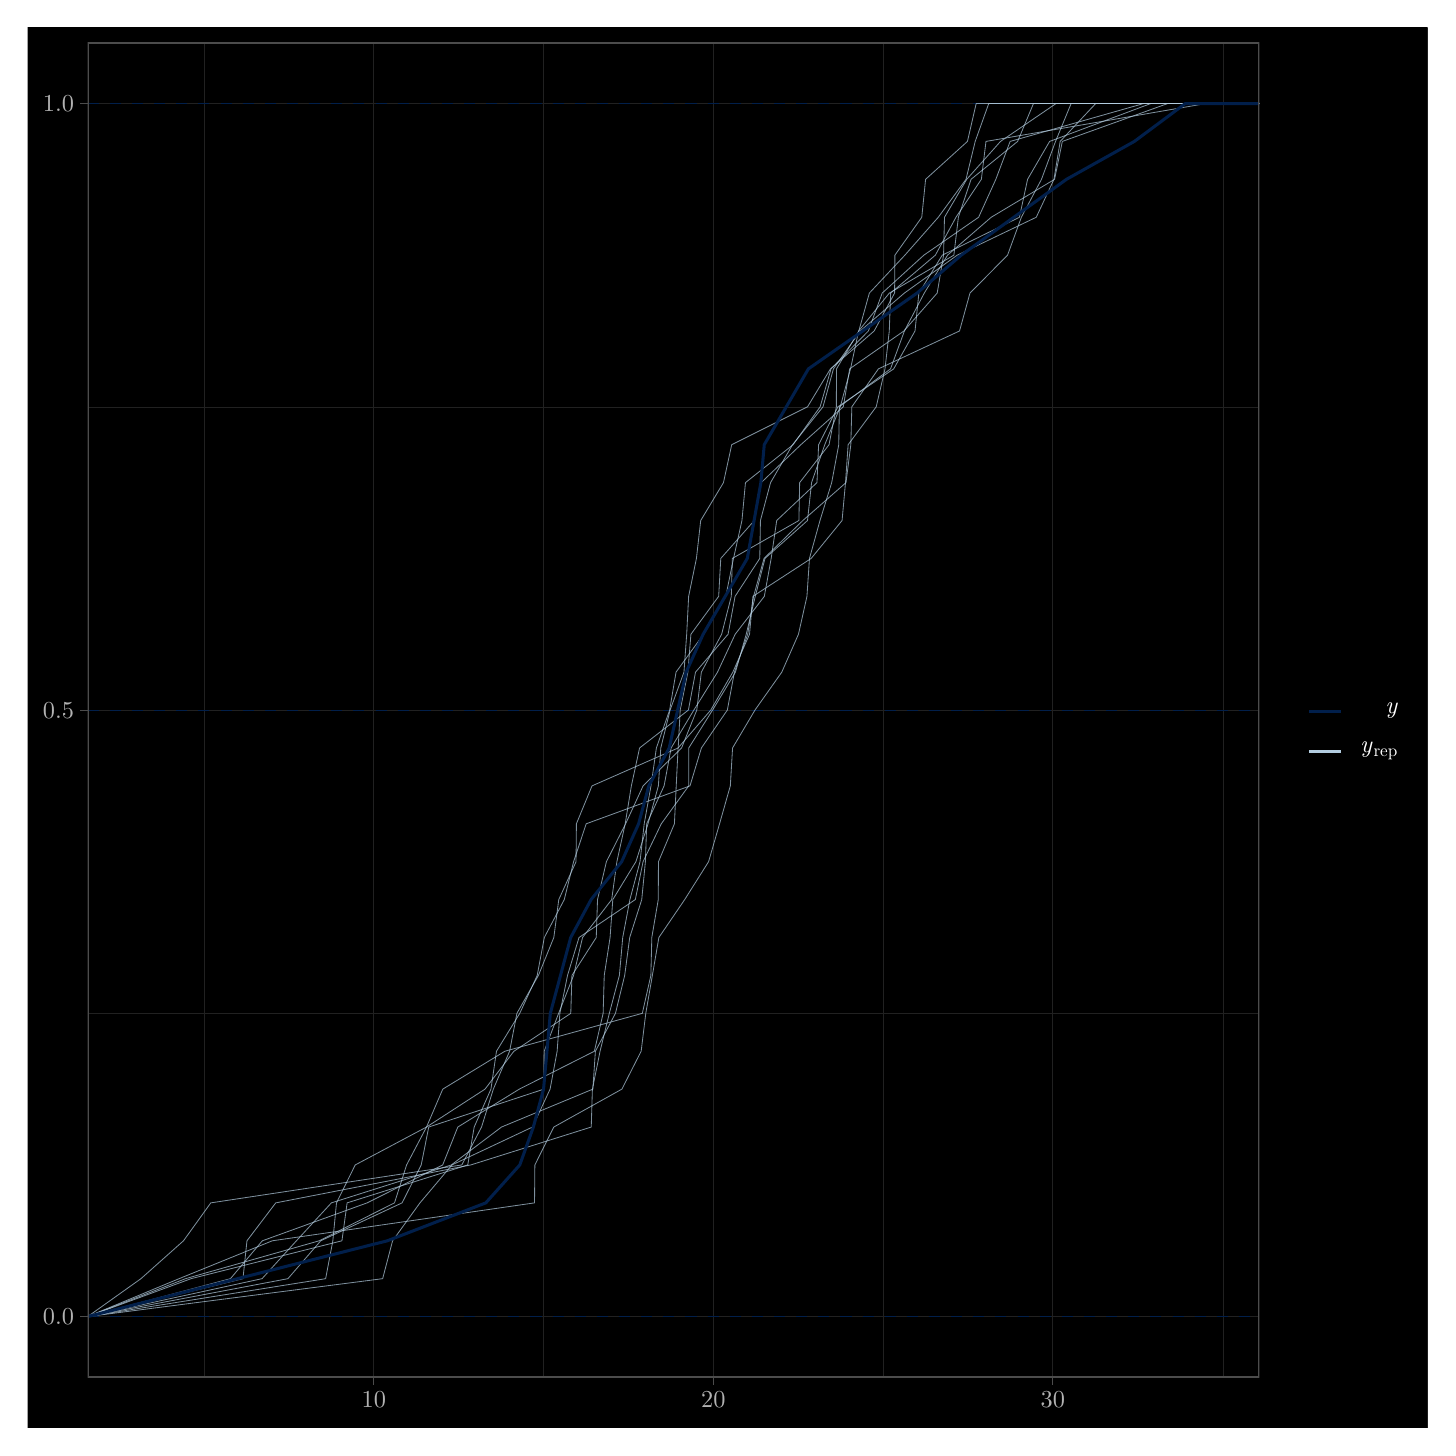
\begin{tikzpicture}[x=1pt,y=1pt]
\definecolor{fillColor}{RGB}{255,255,255}
\path[use as bounding box,fill=fillColor,fill opacity=0.00] (0,0) rectangle (505.89,505.89);
\begin{scope}
\path[clip] (  0.00,  0.00) rectangle (505.89,505.89);
\definecolor{drawColor}{RGB}{0,0,0}
\definecolor{fillColor}{RGB}{0,0,0}

\path[draw=drawColor,line width= 0.6pt,line join=round,line cap=round,fill=fillColor] (  0.00,  0.00) rectangle (505.89,505.89);
\end{scope}
\begin{scope}
\path[clip] ( 21.69, 18.22) rectangle (445.03,500.39);
\definecolor{fillColor}{RGB}{0,0,0}

\path[fill=fillColor] ( 21.69, 18.22) rectangle (445.03,500.39);
\definecolor{drawColor}{gray}{0.13}

\path[draw=drawColor,line width= 0.1pt,line join=round] ( 21.69,149.72) --
	(445.03,149.72);

\path[draw=drawColor,line width= 0.1pt,line join=round] ( 21.69,368.89) --
	(445.03,368.89);

\path[draw=drawColor,line width= 0.1pt,line join=round] ( 63.71, 18.22) --
	( 63.71,500.39);

\path[draw=drawColor,line width= 0.1pt,line join=round] (186.41, 18.22) --
	(186.41,500.39);

\path[draw=drawColor,line width= 0.1pt,line join=round] (309.11, 18.22) --
	(309.11,500.39);

\path[draw=drawColor,line width= 0.1pt,line join=round] (431.81, 18.22) --
	(431.81,500.39);

\path[draw=drawColor,line width= 0.3pt,line join=round] ( 21.69, 40.14) --
	(445.03, 40.14);

\path[draw=drawColor,line width= 0.3pt,line join=round] ( 21.69,259.31) --
	(445.03,259.31);

\path[draw=drawColor,line width= 0.3pt,line join=round] ( 21.69,478.47) --
	(445.03,478.47);

\path[draw=drawColor,line width= 0.3pt,line join=round] (125.06, 18.22) --
	(125.06,500.39);

\path[draw=drawColor,line width= 0.3pt,line join=round] (247.76, 18.22) --
	(247.76,500.39);

\path[draw=drawColor,line width= 0.3pt,line join=round] (370.46, 18.22) --
	(370.46,500.39);
\definecolor{drawColor}{RGB}{1,31,75}

\path[draw=drawColor,line width= 0.1pt,dash pattern=on 4pt off 4pt ,line join=round] ( 21.69,259.31) -- (445.03,259.31);

\path[draw=drawColor,line width= 0.2pt,dash pattern=on 4pt off 4pt ,line join=round] ( 21.69, 40.14) -- (445.03, 40.14);

\path[draw=drawColor,line width= 0.2pt,dash pattern=on 4pt off 4pt ,line join=round] ( 21.69,478.47) -- (445.03,478.47);
\definecolor{drawColor}{RGB}{179,205,224}

\path[draw=drawColor,draw opacity=0.70,line width= 0.3pt,line join=round] ( 21.69, 40.14) --
	( 57.05, 53.84) --
	(105.35, 67.53) --
	(132.55, 81.23) --
	(136.92, 94.93) --
	(144.12,108.63) --
	(149.99,122.33) --
	(172.43,136.02) --
	(222.10,149.72) --
	(225.19,163.42) --
	(225.53,177.12) --
	(227.86,190.82) --
	(227.93,204.51) --
	(233.70,218.21) --
	(234.35,231.91) --
	(235.02,245.61) --
	(246.84,259.31) --
	(254.80,273.00) --
	(260.84,286.70) --
	(262.07,300.40) --
	(283.12,314.10) --
	(294.28,327.80) --
	(295.52,341.49) --
	(296.47,355.19) --
	(306.62,368.89) --
	(309.79,382.59) --
	(311.34,396.29) --
	(311.83,409.98) --
	(327.99,423.68) --
	(335.44,437.38) --
	(344.61,451.08) --
	(346.28,464.78) --
	(425.78,478.47) --
	(445.03,478.47);

\path[draw=drawColor,draw opacity=0.70,line width= 0.3pt,line join=round] ( 21.69, 40.14) --
	( 94.04, 53.84) --
	(105.90, 67.53) --
	(135.29, 81.23) --
	(142.21, 94.93) --
	(144.92,108.63) --
	(186.54,122.33) --
	(186.64,136.02) --
	(191.86,149.72) --
	(197.26,163.42) --
	(200.50,177.12) --
	(211.03,190.82) --
	(212.91,204.51) --
	(215.91,218.21) --
	(218.14,231.91) --
	(221.11,245.61) --
	(238.75,259.31) --
	(241.32,273.00) --
	(253.09,286.70) --
	(255.62,300.40) --
	(264.54,314.10) --
	(264.78,327.80) --
	(268.44,341.49) --
	(276.38,355.19) --
	(287.39,368.89) --
	(291.16,382.59) --
	(300.84,396.29) --
	(316.79,409.98) --
	(335.89,423.68) --
	(364.45,437.38) --
	(370.84,451.08) --
	(373.09,464.78) --
	(385.93,478.47) --
	(445.03,478.47);

\path[draw=drawColor,draw opacity=0.70,line width= 0.3pt,line join=round] ( 21.69, 40.14) --
	( 77.79, 53.84) --
	( 79.24, 67.53) --
	( 89.64, 81.23) --
	(160.09, 94.93) --
	(203.64,108.63) --
	(204.06,122.33) --
	(206.83,136.02) --
	(210.18,149.72) --
	(213.81,163.42) --
	(215.02,177.12) --
	(217.61,190.82) --
	(221.27,204.51) --
	(222.78,218.21) --
	(225.23,231.91) --
	(227.18,245.61) --
	(231.97,259.31) --
	(234.28,273.00) --
	(244.22,286.70) --
	(252.26,300.40) --
	(255.06,314.10) --
	(258.10,327.80) --
	(259.37,341.49) --
	(276.57,355.19) --
	(286.36,368.89) --
	(290.29,382.59) --
	(303.79,396.29) --
	(308.78,409.98) --
	(323.83,423.68) --
	(343.62,437.38) --
	(349.84,451.08) --
	(355.00,464.78) --
	(403.27,478.47) --
	(445.03,478.47);

\path[draw=drawColor,draw opacity=0.70,line width= 0.3pt,line join=round] ( 21.69, 40.14) --
	( 40.93, 53.84) --
	( 56.31, 67.53) --
	( 66.17, 81.23) --
	(156.87, 94.93) --
	(164.00,108.63) --
	(168.26,122.33) --
	(174.14,136.02) --
	(176.79,149.72) --
	(184.56,163.42) --
	(190.12,177.12) --
	(191.91,190.82) --
	(198.15,204.51) --
	(198.28,218.21) --
	(203.92,231.91) --
	(235.06,245.61) --
	(235.79,259.31) --
	(238.56,273.00) --
	(239.66,286.70) --
	(249.69,300.40) --
	(250.45,314.10) --
	(262.57,327.80) --
	(265.04,341.49) --
	(279.38,355.19) --
	(294.72,368.89) --
	(297.02,382.59) --
	(316.63,396.29) --
	(328.65,409.98) --
	(330.95,423.68) --
	(331.29,437.38) --
	(339.32,451.08) --
	(351.53,464.78) --
	(371.60,478.47) --
	(445.03,478.47);

\path[draw=drawColor,draw opacity=0.70,line width= 0.3pt,line join=round] ( 21.69, 40.14) --
	(107.67, 53.84) --
	(110.27, 67.53) --
	(111.59, 81.23) --
	(118.35, 94.93) --
	(144.12,108.63) --
	(165.26,122.33) --
	(175.69,136.02) --
	(196.25,149.72) --
	(196.67,163.42) --
	(205.45,177.12) --
	(205.91,190.82) --
	(209.12,204.51) --
	(216.06,218.21) --
	(222.38,231.91) --
	(236.29,245.61) --
	(241.78,259.31) --
	(243.43,273.00) --
	(250.76,286.70) --
	(254.25,300.40) --
	(254.63,314.10) --
	(278.68,327.80) --
	(278.95,341.49) --
	(289.57,355.19) --
	(292.21,368.89) --
	(292.27,382.59) --
	(300.33,396.29) --
	(304.14,409.98) --
	(316.97,423.68) --
	(329.05,437.38) --
	(339.06,451.08) --
	(342.38,464.78) --
	(347.28,478.47) --
	(445.03,478.47);

\path[draw=drawColor,draw opacity=0.70,line width= 0.3pt,line join=round] ( 21.69, 40.14) --
	( 54.72, 53.84) --
	( 88.40, 67.53) --
	(183.15, 81.23) --
	(183.27, 94.93) --
	(190.11,108.63) --
	(214.72,122.33) --
	(221.68,136.02) --
	(223.35,149.72) --
	(225.73,163.42) --
	(228.08,177.12) --
	(237.41,190.82) --
	(246.04,204.51) --
	(250.01,218.21) --
	(253.90,231.91) --
	(254.71,245.61) --
	(262.81,259.31) --
	(272.49,273.00) --
	(278.52,286.70) --
	(281.59,300.40) --
	(282.50,314.10) --
	(286.30,327.80) --
	(290.53,341.49) --
	(293.08,355.19) --
	(293.30,368.89) --
	(311.79,382.59) --
	(316.81,396.29) --
	(323.98,409.98) --
	(332.39,423.68) --
	(348.17,437.38) --
	(371.06,451.08) --
	(373.87,464.78) --
	(411.95,478.47) --
	(445.03,478.47);

\path[draw=drawColor,draw opacity=0.70,line width= 0.3pt,line join=round] ( 21.69, 40.14) --
	( 59.04, 53.84) --
	(113.56, 67.53) --
	(115.43, 81.23) --
	(159.02, 94.93) --
	(161.34,108.63) --
	(167.40,122.33) --
	(169.40,136.02) --
	(177.81,149.72) --
	(184.12,163.42) --
	(186.69,177.12) --
	(193.90,190.82) --
	(197.27,204.51) --
	(201.82,218.21) --
	(239.32,231.91) --
	(243.45,245.61) --
	(252.82,259.31) --
	(255.38,273.00) --
	(260.19,286.70) --
	(262.31,300.40) --
	(266.08,314.10) --
	(280.11,327.80) --
	(295.70,341.49) --
	(297.44,355.19) --
	(297.81,368.89) --
	(307.41,382.59) --
	(336.72,396.29) --
	(340.50,409.98) --
	(354.07,423.68) --
	(359.07,437.38) --
	(366.33,451.08) --
	(371.41,464.78) --
	(377.05,478.47) --
	(445.03,478.47);

\path[draw=drawColor,draw opacity=0.70,line width= 0.3pt,line join=round] ( 21.69, 40.14) --
	( 73.27, 53.84) --
	( 84.80, 67.53) --
	(122.67, 81.23) --
	(149.97, 94.93) --
	(155.43,108.63) --
	(177.65,122.33) --
	(204.77,136.02) --
	(207.94,149.72) --
	(208.34,163.42) --
	(210.45,177.12) --
	(211.43,190.82) --
	(219.78,204.51) --
	(224.16,218.21) --
	(227.90,231.91) --
	(228.77,245.61) --
	(232.14,259.31) --
	(237.15,273.00) --
	(238.13,286.70) --
	(238.84,300.40) --
	(241.65,314.10) --
	(243.20,327.80) --
	(251.42,341.49) --
	(254.40,355.19) --
	(281.80,368.89) --
	(290.08,382.59) --
	(305.88,396.29) --
	(313.26,409.98) --
	(313.37,423.68) --
	(323.08,437.38) --
	(324.46,451.08) --
	(339.58,464.78) --
	(342.74,478.47) --
	(445.03,478.47);

\path[draw=drawColor,draw opacity=0.70,line width= 0.3pt,line join=round] ( 21.69, 40.14) --
	(128.27, 53.84) --
	(131.86, 67.53) --
	(141.75, 81.23) --
	(153.31, 94.93) --
	(182.41,108.63) --
	(188.77,122.33) --
	(191.32,136.02) --
	(192.31,149.72) --
	(195.07,163.42) --
	(199.23,177.12) --
	(219.57,190.82) --
	(222.37,204.51) --
	(228.95,218.21) --
	(238.87,231.91) --
	(238.88,245.61) --
	(247.49,259.31) --
	(255.75,273.00) --
	(259.65,286.70) --
	(262.91,300.40) --
	(266.43,314.10) --
	(281.79,327.80) --
	(283.26,341.49) --
	(288.03,355.19) --
	(293.62,368.89) --
	(297.33,382.59) --
	(300.27,396.29) --
	(311.36,409.98) --
	(334.67,423.68) --
	(336.31,437.38) --
	(340.88,451.08) --
	(357.72,464.78) --
	(363.44,478.47) --
	(445.03,478.47);

\path[draw=drawColor,draw opacity=0.70,line width= 0.3pt,line join=round] ( 21.69, 40.14) --
	( 84.69, 53.84) --
	( 97.11, 67.53) --
	(109.75, 81.23) --
	(153.08, 94.93) --
	(171.21,108.63) --
	(204.23,122.33) --
	(205.14,136.02) --
	(212.39,149.72) --
	(215.73,163.42) --
	(217.54,177.12) --
	(221.89,190.82) --
	(223.21,204.51) --
	(223.68,218.21) --
	(229.97,231.91) --
	(232.51,245.61) --
	(240.73,259.31) --
	(249.27,273.00) --
	(255.65,286.70) --
	(266.19,300.40) --
	(268.66,314.10) --
	(270.66,327.80) --
	(285.21,341.49) --
	(285.80,355.19) --
	(292.78,368.89) --
	(312.93,382.59) --
	(320.64,396.29) --
	(322.03,409.98) --
	(330.48,423.68) --
	(358.37,437.38) --
	(361.31,451.08) --
	(369.27,464.78) --
	(405.84,478.47) --
	(445.03,478.47);
\definecolor{drawColor}{RGB}{1,31,75}

\path[draw=drawColor,line width= 1.1pt,line join=round] ( 21.69, 40.14) --
	(129.97, 67.53) --
	(165.55, 81.23) --
	(177.82, 94.93) --
	(182.73,108.63) --
	(186.41,122.33) --
	(188.86,149.72) --
	(192.54,163.42) --
	(196.22,177.12) --
	(203.59,190.82) --
	(214.63,204.51) --
	(220.76,218.21) --
	(224.44,231.91) --
	(231.81,245.61) --
	(237.94,273.00) --
	(244.08,286.70) --
	(260.03,314.10) --
	(264.94,341.49) --
	(266.16,355.19) --
	(282.11,382.59) --
	(301.75,396.29) --
	(321.38,409.98) --
	(337.33,423.68) --
	(375.36,451.08) --
	(399.90,464.78) --
	(418.31,478.47) --
	(445.03,478.47);
\definecolor{drawColor}{RGB}{76,76,76}

\path[draw=drawColor,line width= 0.6pt,line join=round,line cap=round] ( 21.69, 18.22) rectangle (445.03,500.39);
\end{scope}
\begin{scope}
\path[clip] (  0.00,  0.00) rectangle (505.89,505.89);
\definecolor{drawColor}{RGB}{178,178,178}

\node[text=drawColor,anchor=base east,inner sep=0pt, outer sep=0pt, scale=  0.88] at ( 16.74, 37.11) {0.0};

\node[text=drawColor,anchor=base east,inner sep=0pt, outer sep=0pt, scale=  0.88] at ( 16.74,256.28) {0.5};

\node[text=drawColor,anchor=base east,inner sep=0pt, outer sep=0pt, scale=  0.88] at ( 16.74,475.44) {1.0};
\end{scope}
\begin{scope}
\path[clip] (  0.00,  0.00) rectangle (505.89,505.89);
\definecolor{drawColor}{RGB}{76,76,76}

\path[draw=drawColor,line width= 0.3pt,line join=round] ( 18.94, 40.14) --
	( 21.69, 40.14);

\path[draw=drawColor,line width= 0.3pt,line join=round] ( 18.94,259.31) --
	( 21.69,259.31);

\path[draw=drawColor,line width= 0.3pt,line join=round] ( 18.94,478.47) --
	( 21.69,478.47);
\end{scope}
\begin{scope}
\path[clip] (  0.00,  0.00) rectangle (505.89,505.89);
\definecolor{drawColor}{RGB}{76,76,76}

\path[draw=drawColor,line width= 0.3pt,line join=round] (125.06, 15.47) --
	(125.06, 18.22);

\path[draw=drawColor,line width= 0.3pt,line join=round] (247.76, 15.47) --
	(247.76, 18.22);

\path[draw=drawColor,line width= 0.3pt,line join=round] (370.46, 15.47) --
	(370.46, 18.22);
\end{scope}
\begin{scope}
\path[clip] (  0.00,  0.00) rectangle (505.89,505.89);
\definecolor{drawColor}{RGB}{178,178,178}

\node[text=drawColor,anchor=base,inner sep=0pt, outer sep=0pt, scale=  0.88] at (125.06,  7.21) {10};

\node[text=drawColor,anchor=base,inner sep=0pt, outer sep=0pt, scale=  0.88] at (247.76,  7.21) {20};

\node[text=drawColor,anchor=base,inner sep=0pt, outer sep=0pt, scale=  0.88] at (370.46,  7.21) {30};
\end{scope}
\begin{scope}
\path[clip] (  0.00,  0.00) rectangle (505.89,505.89);
\definecolor{fillColor}{RGB}{0,0,0}

\path[fill=fillColor] (456.03,231.74) rectangle (500.39,286.87);
\end{scope}
\begin{scope}
\path[clip] (  0.00,  0.00) rectangle (505.89,505.89);
\definecolor{fillColor}{RGB}{0,0,0}

\path[fill=fillColor] (461.53,251.70) rectangle (475.98,266.15);
\end{scope}
\begin{scope}
\path[clip] (  0.00,  0.00) rectangle (505.89,505.89);
\definecolor{drawColor}{RGB}{1,31,75}

\path[draw=drawColor,draw opacity=0.70,line width= 0.3pt,line join=round] (462.97,258.93) -- (474.53,258.93);
\end{scope}
\begin{scope}
\path[clip] (  0.00,  0.00) rectangle (505.89,505.89);
\definecolor{drawColor}{RGB}{1,31,75}

\path[draw=drawColor,line width= 1.1pt,line join=round] (462.97,258.93) -- (474.53,258.93);
\end{scope}
\begin{scope}
\path[clip] (  0.00,  0.00) rectangle (505.89,505.89);
\definecolor{fillColor}{RGB}{0,0,0}

\path[fill=fillColor] (461.53,237.24) rectangle (475.98,251.70);
\end{scope}
\begin{scope}
\path[clip] (  0.00,  0.00) rectangle (505.89,505.89);
\definecolor{drawColor}{RGB}{179,205,224}

\path[draw=drawColor,draw opacity=0.70,line width= 0.3pt,line join=round] (462.97,244.47) -- (474.53,244.47);
\end{scope}
\begin{scope}
\path[clip] (  0.00,  0.00) rectangle (505.89,505.89);
\definecolor{drawColor}{RGB}{179,205,224}

\path[draw=drawColor,line width= 1.1pt,line join=round] (462.97,244.47) -- (474.53,244.47);
\end{scope}
\begin{scope}
\path[clip] (  0.00,  0.00) rectangle (505.89,505.89);
\definecolor{drawColor}{RGB}{255,255,255}

\node[text=drawColor,anchor=base west,inner sep=0pt, outer sep=0pt, scale=  0.88] at (490.62,257.89) {\itshape y};
\end{scope}
\begin{scope}
\path[clip] (  0.00,  0.00) rectangle (505.89,505.89);
\definecolor{drawColor}{RGB}{255,255,255}

\node[text=drawColor,anchor=base west,inner sep=0pt, outer sep=0pt, scale=  0.88] at (481.48,243.84) {\itshape y};

\node[text=drawColor,anchor=base west,inner sep=0pt, outer sep=0pt, scale=  0.62] at (486.32,242.51) {r};

\node[text=drawColor,anchor=base west,inner sep=0pt, outer sep=0pt, scale=  0.62] at (488.73,242.51) {e};

\node[text=drawColor,anchor=base west,inner sep=0pt, outer sep=0pt, scale=  0.62] at (491.47,242.51) {p};
\end{scope}
\end{tikzpicture}
}
        \end{figure}
    \end{column}
\end{columns}
\end{frame}
